\documentclass[output=book,
%  colorlinks,citecolor=brown
%  ,draft
%  ,draftmode,
%  booklanguage=german,
		  ]{langscibook}
%%%%%%%%%%%%%%%%%%%%%%%%%%%%%%%%%%%%%%%%%%%%%%%%%%%%
%%%          additional packages                 %%%
%%%%%%%%%%%%%%%%%%%%%%%%%%%%%%%%%%%%%%%%%%%%%%%%%%%%
\author{Maria Zielenbach}
\title{Half silver, half gold}
\subtitle{Modole folk stories and a first sketch grammar}
\BackBody{This collection contains ten folk stories in Modole, a Papuan language of the North Moluccas in eastern Indonesia. They were first published in 1916 by Dutch missionary G.J. Ellen and appear here re-edited, translated into English and with interlinear glossings.

In addition, the book offers the first grammatical description of Modole, as well as information on the Modole people and their culture and environment.
}
\renewcommand{\lsISBNdigital}{978-3-96110-548-9}
\renewcommand{\lsISBNhardcover}{978-3-98554-168-3}
\BookDOI{10.5281/zenodo.17511782}
\typesetter{Maria Zielenbach, Christian Döhler}
\proofreader{Matthew Korte}
\lsCoverTitleSizes{45pt}{15mm}
\renewcommand{\lsSeries}{otc}
\renewcommand{\lsSeriesNumber}{6}
\renewcommand{\lsID}{542}
\dedication{I humbly dedicate this book to the original narrators of the stories whose names have been lost in history. \\ I hope this book presents your stories in a way that you would have appreciated.}

\renewcommand{\lsDedicationFont}{\fontsize{15pt}{8mm}\selectfont}
\renewcommand{\lsYear}{2026}

\input{localpackages.tex}
\input{localhyphenation.tex}
\addbibresource{localbibliography.bib}
%%%%%%%%%%%%%%%%%%%%%%%%%%%%%%%%%%%%%%%%%%%%%%%%%%%%
%%%             Frontmatter                      %%%
%%%%%%%%%%%%%%%%%%%%%%%%%%%%%%%%%%%%%%%%%%%%%%%%%%%%
% \includeonly{chapters/sketch}
\begin{document}
% \newcommand{\addtext}[2]{
%     \chapter{#2}\label{text:#1}
%     \section*{Metadata}
%     \input{chapters/#1/meta_#1.tex}
%     \section*{Summary \& background}
%     \input{chapters/#1/intro_#1.tex}
%     \section*{Parallel Text}
%     \input{chapters/#1/translation_#1.tex}
%     \section*{Glossed text}
%     \input{chapters/#1/glosses_#1.tex}
% }

\newcommand{\til}{$\sim$}
\newcommand{\pnh}{Proto-North Halmahera}
\newcommand{\nhl}{North Halmahera languages}
\newcommand{\nhll}{North Halmahera language}
\newcommand{\cnh}{Core North Halmahera}
\newcommand{\cnhl}{Core North Halmahera languages}
\newcommand{\cnhll}{Core North Halmahera language}
\newcommand{\pcnh}{Proto-Core North Halmahera}
\newcommand{\mnhl}{Mainland North Halmahera languages}
\newcommand{\pmnh}{Proto-Mainland North Halmahera}

\hypersetup{hypertexnames=false}%fixes the wrong hyperlinks after \setcounter{chapter}{0} in main.tex

\newcommand{\textref}[1]{Text~\ref{#1}}%xref command for texts
\renewcommand{\sectref}[1]{Section~\ref{#1}}%xref command sections

\examplesitalics%morpheme line of example appears in italics
%\renewcommand{\exfont}{\itshape}%text line of examples appears in italics


\maketitle
\frontmatter
\currentpdfbookmark{Contents}{name} % adds a PDF bookmark
{\sloppy\tableofcontents}
%% remove the % in the following lines if your book has these elements
% \include{chapters/preface}
 \addchap{\lsAcknowledgementTitle}

When G.J. Ellen published the texts edited in this book in 1916 he did not consider it necessary to acknowledge their narrators or even record their names. This injustice cannot be undone and I wish to thank the narrators with all my heart. Without them this book as well as my research would not be possible.

The edition of the texts in this book commenced as a side project to my PhD project about the linguistic history of the North Halmahera languages (supported by the OUTOFPAPUA project funded by the European Research Council (grant agreement no. 848532)). Modole is the least described of the North Halmahera languages. My analysis of the texts initially served the purpose of including Modole data in my study. This work is addressed to linguists and members of the Modole community who wish to learn more about the language. I pursue no religious or ideological goals.

I thank Christian Döhler for making me aware of \textit{Open Text Collections} and his continuous encouragment and support in publishing this book; and Uri Tadmor of Brill for the permission to republish the texts.
I wish to thank Annika Schiefner, Antoinette Schapper, Jacob Menschel, Norea Beaujean, Silvie Strauß, and especially Robert Tegethoff for reading early drafts of chapters; two reviewers for their helpful comments; and Lena Pointner and my parents for their persistent enthusiasm. 
I further wish to thank Edward Kotynski for our discussions on all things Tabaru and North Halmahera in general; and Dalan Perangin Angin for answering numerous questions on Pagu.

My final thanks go to a Modole speaker who patiently answered my weird questions about the texts and Modole language and culture.\footnote{Due to paternalistic privacy laws of the European Union, I am not allowed to name my language informant. They are not allowed to deanonymize themself either.} Their views do not represent the whole Modole community, which was not further involved in the creation of this work.
 \addchap{\lsAbbreviationsTitle}

\begin{tabularx}{.45\textwidth}{lQ}
    \textsc{<}&derived from\\
    1&first person\\
    2&second person\\
    3&third person\\
    \textsc{a}&actor\\
    \textsc{appl}&applicative\\
    \textsc{caus}&causative\\
    \textsc{class}&numeral classifier\\
    \textsc{conn}&connective\\
    \textsc{cond}&conditional\\
    CV&reduplication of first syllable \\
    (C)V(C)V& reduplication of first two syllables \\
    \textsc{dir}&directional\\
    \textsc{dist}&distal\\
    \textsc{emph}&emphatic\\
    \textsc{ex}&exclusive\\
    \textsc{excl}&exclamative\\
    \textsc{exist}&existential\\
    \textsc{f}&feminine\\
    \textsc{foc}&focus\\
    \textsc{hon.fem}&feminine honorific\\
    \textsc{hpl}&human plural\\
    \textsc{hum}&human \\
    \textsc{in}&inclusive\\
    \textsc{itv}&itive\\
\end{tabularx}
\begin{tabularx}{.45\textwidth}{lQ}
    k.o.&kind of\\
    \textsc{lim}&limitative\\
    \textsc{loc}&locational\\
    \textsc{locv}&locative\\
    \textsc{m}&masculine\\
    \textsc{mid}&middle\\
    \textsc{mod}&modal marker\\
    \textsc{n}&initial /ng/ found in some directionals\\
    \textsc{neg}&negation\\
    \textsc{nh}&non-human\\
    \textsc{nm}&noun marker\\
    \textsc{perf}&perfect\\
    \textsc{pcnh}&Proto-Core North Halmahera \\
    \textsc{pl}&plural\\
    \textsc{poss}&possessive\\
    \textsc{pro}&personal pronoun\\
    \textsc{proh}&prohibitive \\
    \textsc{prox}&proximate\\
    \textsc{rdpl}&reduplication\\
    \textsc{rnm}&relational noun marker\\
    \textsc{sg}&singular\\
    \textsc{u}&undergoer\\
    \textsc{ven}&ventive\\
    \textsc{vpl}&verbal plural \\
    \\
\end{tabularx}

\mainmatter

%%%%%%%%%%%%%%%%%%%%%%%%%%%%%%%%%%%%%%%%%%%%%%%%%%%%
%%%             Chapters                         %%%
%%%%%%%%%%%%%%%%%%%%%%%%%%%%%%%%%%%%%%%%%%%%%%%%%%%%
\part{Preliminaries}
    \chapter{Introduction}\label{chapter:intro}
    The texts in this collection were recorded among the Modole people of Halmahera Island at the beginning of the twentieth century in the context of the mission of the Utrechtse Zendingsvereeniging (UZV). They were published by the missionary G.J. Ellen under the title \textit{Verhalen en fabelen in het Modòle met vertalingen} (`Tales and fables in Modole with translations') in the journal \textit{Bijdragen tot de Taal-, Land- en Volkenkunde van Nederlandsch-Indië} in 1916. Together with a Modole wordlist, published in the same journal, and another wordlist\footnote{One of the Holle lists, published in \citet{stokhof1980, stokhof1980a}.} they remain to this day the only printed publications in or about the Modole language. The aim of this book is to make the texts accessible to a larger linguistic audience. 

The context in which the texts were collected is not documented. Neither the name(s) of the narrator(s) nor the exact time and place of recording is known. To amend this lack of documentation I provide background information about the Modole and their language (Chapter \ref{chap:Modole}), about G.J. Ellen and his mission (Chapter \ref{chap:Ellen}), and about the texts themselves (Chapter \ref{chap:stories}). 
I also include an extensive sketch grammar (Chapter \ref{chapter:sketch}) -- the first published grammatical description of Modole. 
Next are the 10 texts (Part \ref{part:texts}); each with a short introduction and summary, Ellen's original Dutch translation, my English translation, and the interlinearlized Modole text. Notes on the texts are provided in footnotes.
Throughout this book, I refer to the Malay varieties spoken in Indonesia as \textit{Indonesian}, even though the texts precede the Indonesian nation state. 

\chapter{The Modole, their land and their language}
\label{chap:Modole}

In this chapter, I provide information about the history of the Modole people (\sectref{subsec:people}), their traditional religious customs and folk tale traditions (\sectref{subsec:folk_religion}), their geographical surroundings (\sectref{subsec:land}) and their language (\sectref{subsec:land}).
Much of this information comes from colonial sources, often written in the condescending and patronizing tone common to these sources. 

\section{History of the Modole people}
\label{subsec:people}

The Modole are one of the ethnic groups (Indonesian \textit{suku}) of the northern peninsula of Halmahera island. Halmahera is part of the North Moluccas in modern-day eastern Indonesia. The Modole have occupied an area along the upper Kao river in the modern district Kao Barat since at least the 17th century. They were formerly subjects of the Sultan of Ternate, an island to the west of Halmahera that gained power and wealth through the spice trade. The North Moluccas are the native home of the clove tree (\textit{Syzygium aromaticum}) and traders from Java, India, China, Arabia and Europe visited the islands in medival and early modern times to buy the precious commodity.  

Since they lived far in the interior of Halmahera, the Modole remained outside the focus of European colonizers longer than their neighbors. 
They are first mentioned in an European source in a report by the retiring Dutch Governor of Ternate, Jacob Lobs, dating to 1686 (published in \cite{dam1931}). Lobs mentions a place-name called \textit{Mondole} two hours away from Pagu. The inhabitants are described as ``wilt, schuw en vreesagtig'' (`wild, shy and apprehensive', \cite[113]{dam1931}). There were 30 able-bodied men among them.

After Lobs' report, the Modole are not mentioned in European sources until the 19th century.
For the end of the 19th century, \citet[62, 66]{declercq1890} states that the \textit{sangaji} (a kind of local ruler) of the district Modole (spelled Madolé) is subject to the \textit{sangaji} of Kao Bay, and that the \textit{negorij} (small village) Madolé does not pay regular taxes to the Sultan of Ternate (its formal ruler).

According to \citet{ellen1916}, there were around 2,000 Modole at the beginning of the 20th century.\footnote{Precise numbers of Modole congregation members can be found in \citet[136]{utrechtschezendingvereeniging1915}. I decided against including them here since they only cover Christians and hence a fraction of the total Modole population.}
In 1909, the \textit{Civiele Gezaghebber} (administrator) of the east coast of Halmahera, G.J.J. de Jongh, included several traditions about the origin of the Modole in one of his reports. 
He states that they are related to the Tabaru and ``came from elsewhere with them, likely from Sulawesi, because the Madole are still called `orang bugis' [Buginese]'' \citep[755]{dejongh1909}.\footnote{``met deze van elders kwamen, waarschijnlijk van Celebes, want de Madolé's worden thans nog wel door de anderen `orang boegies' genoemd''}
There were immigrants from Sulawesi in the area around the time, but a connection to the Modole is not mentioned elsewhere. 
De Jongh further reports that the villages Gogala ma lako, Bailengit and Tolabit, which today are inhabited by Modole, were founded by people who originally lived around Lake Lina (see Map in \figref{fig:villages}). Other inhabitants of the Lake Lina area became the modern-day Tobelos, implying that Modole and Tobelo have a shared origin \citep[756]{dejongh1909}. The story is considered implausible by \citet[125-126]{vanfraassen1980} on linguistic grounds. 
According to \citet[756]{dejongh1909}, the Modole from the villages of Toegoeis (Tuguis), Hoekoem (Soahukum), Sengadji (Soasengaji) and Taraut (Torawat) originally lived with the Gamkonora and were attracted by the Sago forests in the Modole region. \citet{leith1999} also corroborates that the population of Torawat were immigrants.

The Modole had an infamous reputation in the early 20th century.
In 1906, UZV missionary G.J. Ellen reported that he had not been able to visit the Modole yet ``since all other tribes are scared of these people''\footnote{``omdat alle anderen stammen bang zijn voor deze menschen''} \citep[166]{ellen1906}.
De Jongh, however, had visited the Modole and Ellen states that ``from his reports, as well as those of the gurus\footnote{helpers from other parts of Indonesia (MZ)} and my own observations it seems that this tribe is not as hostile as thought. It mostly seems to be incitement of the Mohammedans, who want to use this rather large tribe in their hatred of Christianity and the government''\footnote{``Uit zijne mededeelingen, alsmede die der goeroes en mijn eigen bevindingen is mij gebleken dat die stam niet zoo vijandig is als wel werd vermoed. Het schijnt veelal opstokerij van de Mohammedanen te zijn, die dezen tamelijk grooten stam willen gebruiken in hun haat tegen het Christendom en het Gouvernement.''} \citep[166]{ellen1906}.
It must be noted that local Muslims were seen as antagonists by the Dutch missionaries and were therefore accused of all manner of misdeeds (compare \cite[6-7]{ellennda} and the preface of \cite{ellennd}). 
In any case, the Modole did not live up to the stories that Ellen had been told about them. 
He further reports that Modole from the villages of Perseba and Bailengit wished to become Christians and later, gurus were placed there \citep[166]{ellen1906}.\footnote{For more information on the mission among the Modole see Chapter \ref{chap:Ellen}.}  
%add population numbers from 1915_28_8_9

After the Indonesian independence, interest in the Modole did not increase.
\citet{leith1999} outlines the recent history of the Modole and appears to be the only ethnological study concerning them. A short video filmed in the Modole village Soamahukum in 2022 can be found at \url{https://youtu.be/xfkSKQTlDpQ?si=wzV9ST8u8bBEjQob} (accessed 4 October 2025). The map in Figure \ref{fig:villages} shows the location of the original Modole villages today.\footnote{Due to the transmigration program of the Indonesian government, villages of the same name now exist further south in the Malifut area (see \cite{leith1999}).}

\begin{figure}
    \centering
    \includegraphics[width=1\linewidth]{figures/Modole.png}
    \caption{Position of the original Modole villages today (the village of Soasengaji is now called Sangaji Jaya) [created by the author]}
    \label{fig:villages}
\end{figure}

Unfortunately, no detailed accounts about the daily life of the Modole around the time when the texts were collected are available. When the texts in this collection were recorded, many Modole had only recently come into closer contact with the Dutch colonialists and their Christian faith that they were now encouraged to adopt.
Reports by civil colonial administrators focus on population numbers and taxes, while missionaries like Ellen mostly reported on the progress of Christianization and the changes brought about by it.
For example, one of the prerequisites for becoming Christian was to settle permanently in a village and give up foraging. Before, people had often spent extensive periods of time in their inland gardens and created income by collecting dammar gum \citep[159]{ellen1908}. The most comprehensive ethnographic description of a North Halmaheran ethnic group was published by Ellen's missionary colleague \citet{hueting1921,hueting1922} about the Tobelo people. Many aspects of his description pertain to the Modole as well. 



\section{Modole folk tale tradition and traditional religious beliefs}
\label{subsec:folk_religion}

We may call the texts published in Ellen's (\citeyear{ellen1916}) collection `folk stories'. They show similarities to folk stories collected among other North Halmahera groups. For example, the story \textit{O Biara} (Chapter \ref{chapter:text07}) strongly resembles the story \textit{O Radja-Moloko de o ngo Namo-Bilala ma ngadje-ngadje} (`The story of Raja-Moloko and Namo-Bilala') in \posscitet{fortgens1928} Tabaru story collection.\footnote{Notably, there is no version of the `Monkey and Tortoise' story popular throughout Eastern Indonesia, see \citet[411]{vanstaden2000} for a Tidore version and information on the story in general.} 

Before their conversion to Christianity, the Modole adhered to a religion similar to those of other North Halmaheran ethnic groups. There is no comprehensive study of Modole traditional religious beliefs. Some information is found in \citet{leith1999}.\footnote{Note that the paper is concerned with southern Modole villages, while the texts likely were collected in the northern villages.} Elements of these traditional religious beliefs are still preserved today and have been incorporated into local Christianity. The traditional religious beliefs include ancestor worship as well as the belief in a number of spirits and other supernatural beings.
Some of them populate the enchanted country in which the stories in this collection are set; among them the \textit{to'ata} (a kind of evil spirit), the \textit{goda} spirit, \textit{jini} `jinns' and \textit{widadari} `nymphs' (see footnotes in respective texts for more information). 

The interior of Halmahera may appear remote today but historically it was connected to the world through the spice trade and the Modole adopted many foreign cultural practices.
The belief in jinns had been adopted from Muslims at some point in time. Immigrants from Ternate and local converts lived in the coastal settlements of Kao bay. The protagonists of the text \textit{Naga o njawa ja mididi jo puaha} (Chapter \ref{chapter:text08}) are Muslims.
The word \textit{widadari} is of Javanese (and ultimately Sanskrit) origin. Javanese culture was brought to Ternate by traders and spread from there to Halmahera (see \citet{schapper2025}). 
\citet[12-13]{hueting1908a} believed that many of the Tobelo stories originated elsewhere and observed similarities to stories collected on the Sangir islands north of Sulawesi.

The missionaries further noted that some of the folk stories they recorded appear to be a combination of several stories (see for example \cite[454]{vanbaarda1904}). This was still observed in 2000 by \citet[337]{vanstaden2000}. A candidate for such a combined story is \textref{chapter:text01}.

The \textit{Sitz im Leben} of the stories is not documented.
The only information regarding the function and meaning of folk tales for the daily lives of the people of North Halmahera at the beginning of the 20th century is found in the introduction of Hueting's (\citeyear{hueting1908a}) Tobelo story collection:

\begin{quote}
 ``These stories do not play an important role in the lives of the Tobelo. Only few know them and one can spend quite a long time among them without knowing that such stories are known at all. They are not told during public events or feasts but rather in private circles. Usually this happens -- only in a few families -- at night, when they have already gone to bed but cannot fall asleep. [...] Sometimes someone will say: I know a story. Just tell it, others reply. The story teller starts by saying ``Stories''  and every one replies ``téde'', which means ``we are listening''. Then the story follows. Afterwards the story is dissected, or someone else feels inspired to tell one too, and so it continues until everybody has fallen asleep. [...] In fact, the stories do not feel as real to the people as one may think. [...] Also, what one reads about supernatural matters or about the spirit world and the life hereafter hardly corresponds to the common belief about these things, and I have never known anyone to be the least disturbed by what appears in the stories in this respect, or that anything is claimed based on them. They are an amusement, nothing more.'' \citep[13]{hueting1908a} (my translation)
\end{quote}

One interesting feature of the stories is the large number of assertive female protagonists. Most characters and almost all protagonists are women or girls. For more motives found in the stories, see the footnotes to the interlinearized texts. Several common motives of Loloda folk tales, some of which also occur in the Modole stories, are discussed in \citet[322--329]{vanbaarda1904}.


\section{The Modole land}
\label{subsec:land}

The most detailed description of geographic surroundings of the Modole around the time the texts were recorded can be found in \citet{campen1884}. Ellen's (\citeyear{ellennd}) report of one of his trips to the Modole villages provides further information.
According to \citet[277]{campen1884}, the first Modole village is reached from the coast after eight hours' walk.\footnote{Campen calls it Babawat. This name is not recorded elsewhere.}
The interior of Halmahera was dominated by thick rain forest, as it is today.  Most parts of the island are covered by mountain ranges with several active volcanoes, but the Modole land around the Kao river forms a valley with marshy soil. Rivers constitute the main means of transportation. The largest of these is the Kao river (see Figure \ref{fig:Kao_river}).\footnote{Link to the photograph: \url{http://hdl.handle.net/1887.1/item:829037} (accessed 4 October 2025)} Traveling by boat plays a role in almost all of the stories in the collection. 
Sago forests provided the staple food source at the time (compare \textref{chapter:text03} and \textref{chapter:text05}), supplemented by fishing and hunting (compare \textref{chapter:text02}, \textref{chapter:text03}, see \cite[252-274]{hueting1922}).

\begin{figure}
    \centering
    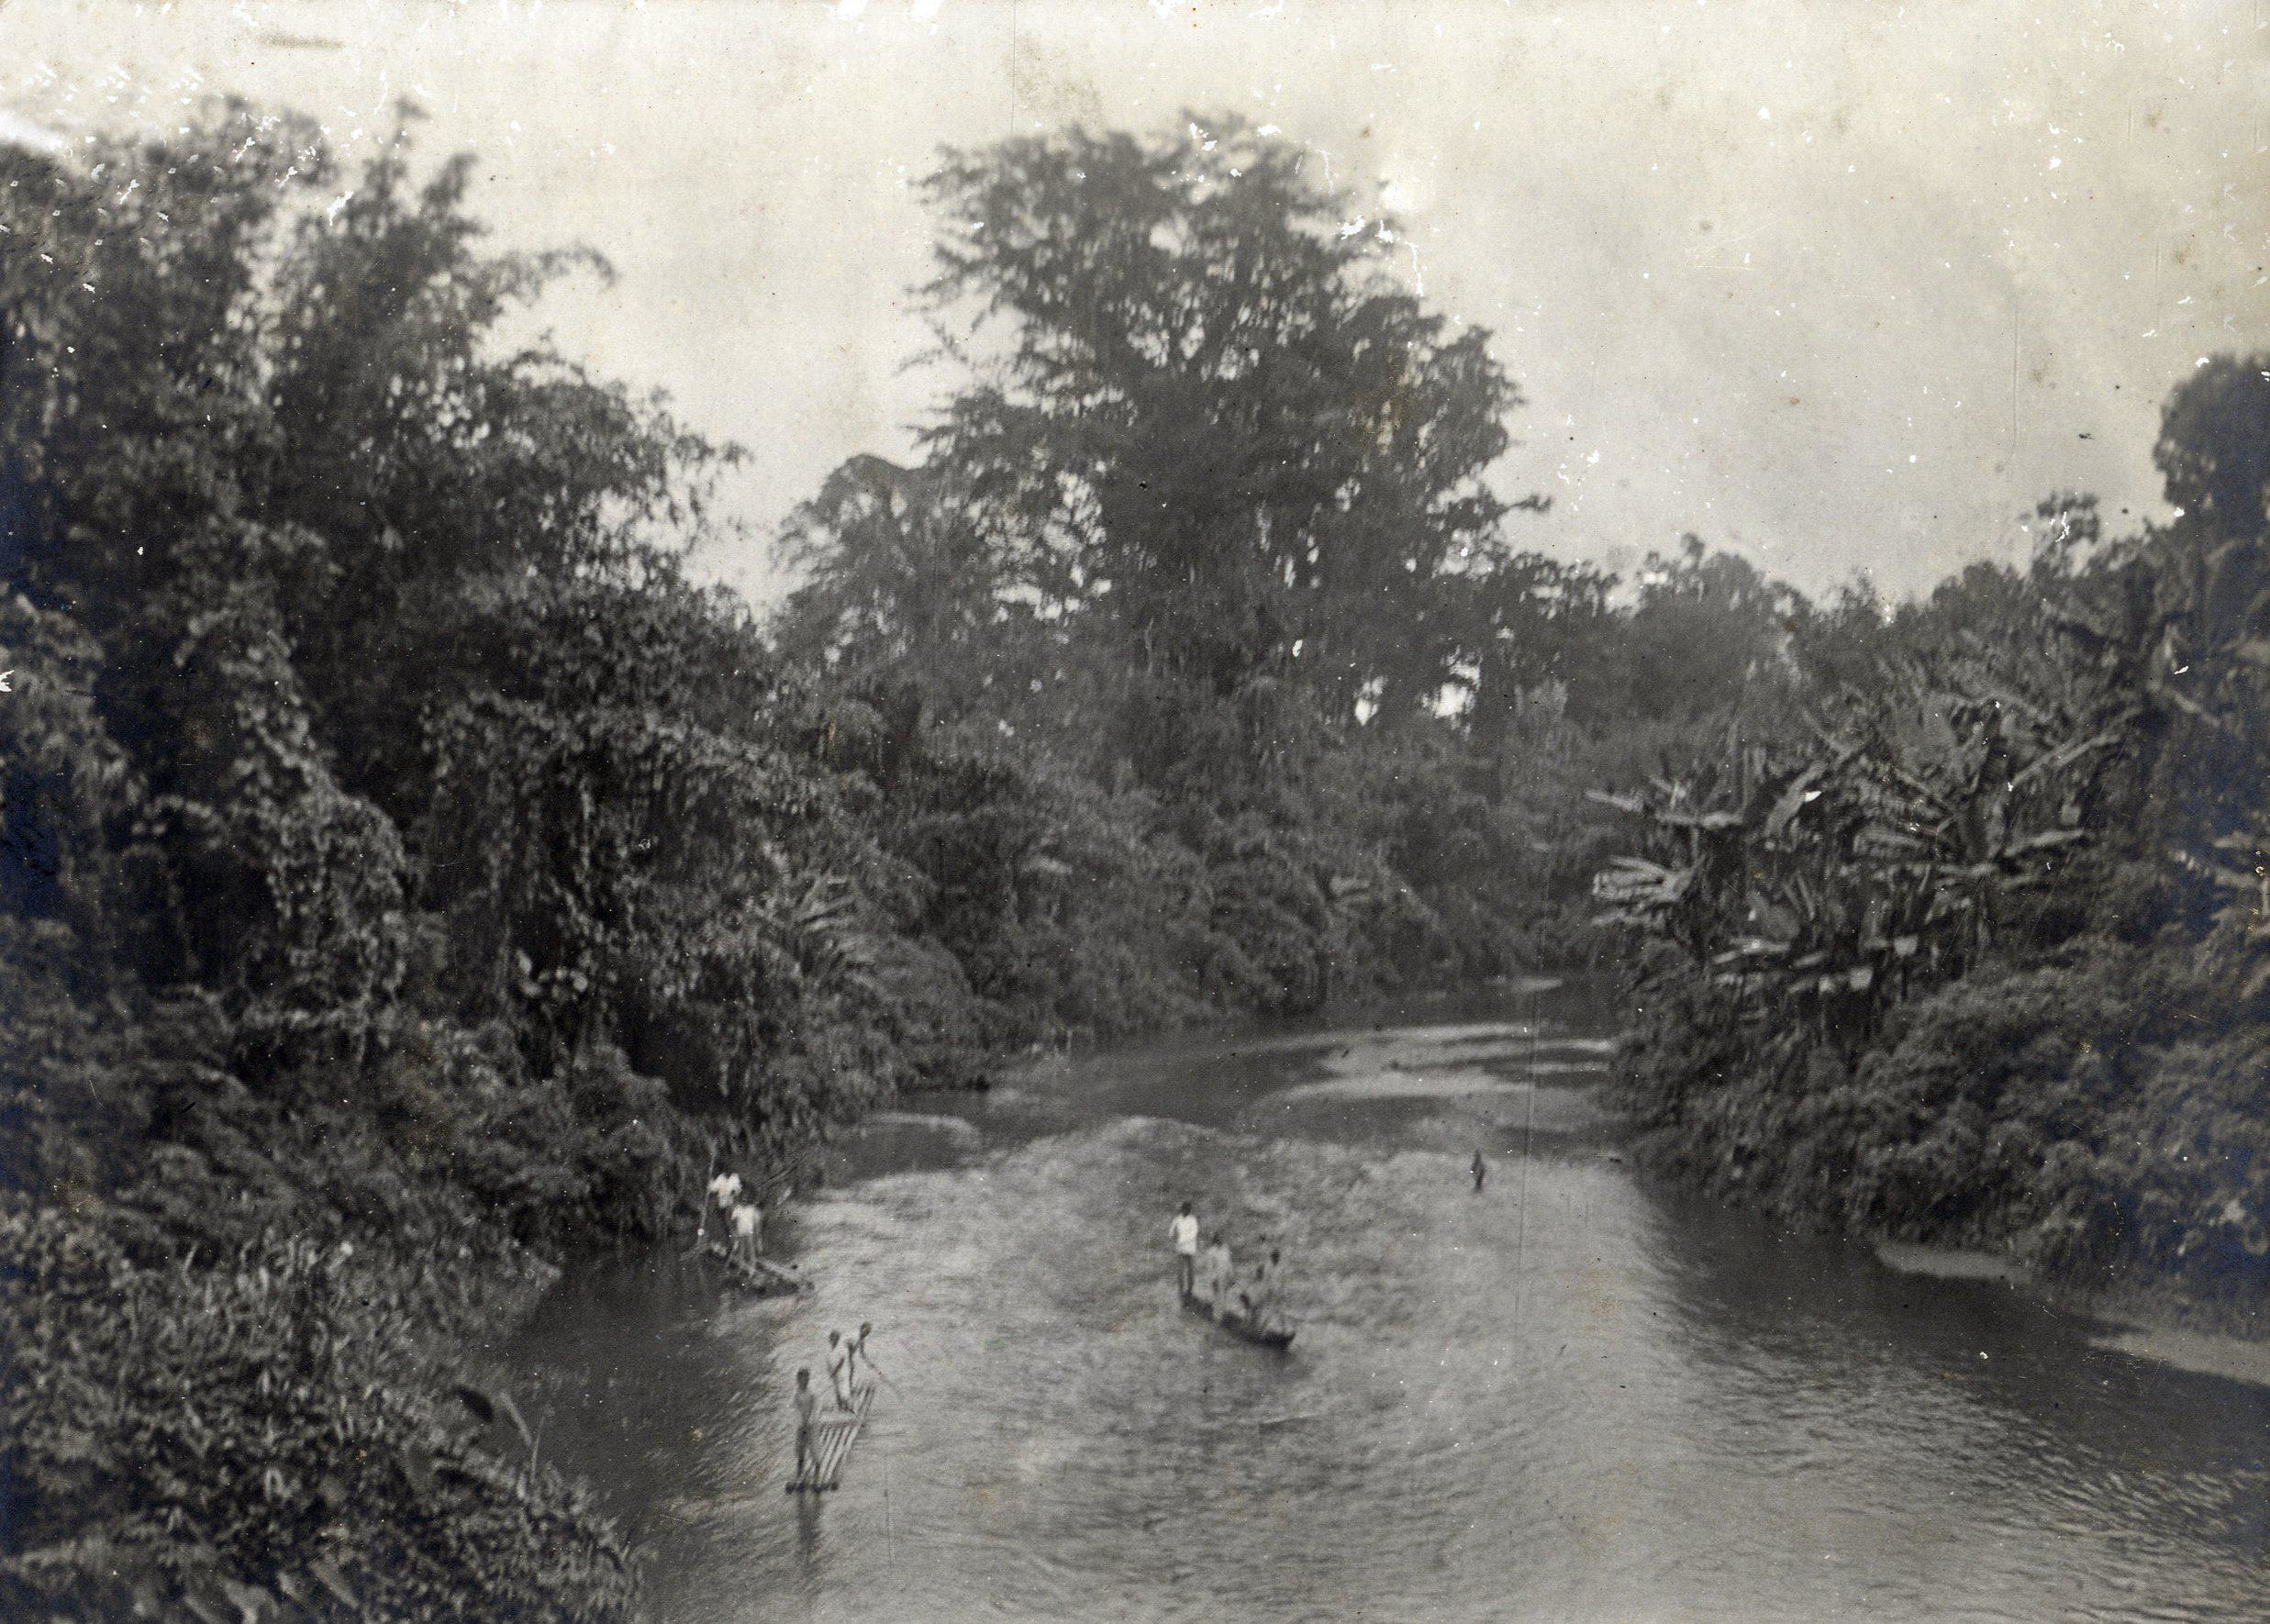
\includegraphics[width=1\linewidth]{figures/Kao_river.png}
    \caption{Photograph titled \textit{Kano op de Kaoe-rivier in Halmahera} (`Canoe on the Kao river on Halmahera') from the KITLV archive (dated ca. 1910). [Public domain]}
    \label{fig:Kao_river}
\end{figure}

Modole villages were centered around a community house that also served as village temple. Houses were made of bamboo and built on poles (compare \textref{chapter:text09}). A photograph of such a house (though belonging to a family from the neighboring ethnic group called ``Tugutil''\footnote{``Tugutil'' is commonly used for Tobelo-speaking groups living in the interior of Halmahera. According to \citet{duncan1997} the name is regarded as offensive by people it is applied to.}) from the KITLV archive in Leiden is displayed in Figure \ref{fig:Tugutil_house}.\footnote{Link to the photograph: \url{http://hdl.handle.net/1887.1/item:827860} (accessed 4 October 2025)} 
The people also spent an extensive amount of time in their gardens (compare \textref{chapter:text02}, \textref{chapter:text04}) that were cultivated through swidden agriculture (see \cite{leith1999}, \cite[214-215]{hueting1922}). 

\begin{figure}
    \centering
    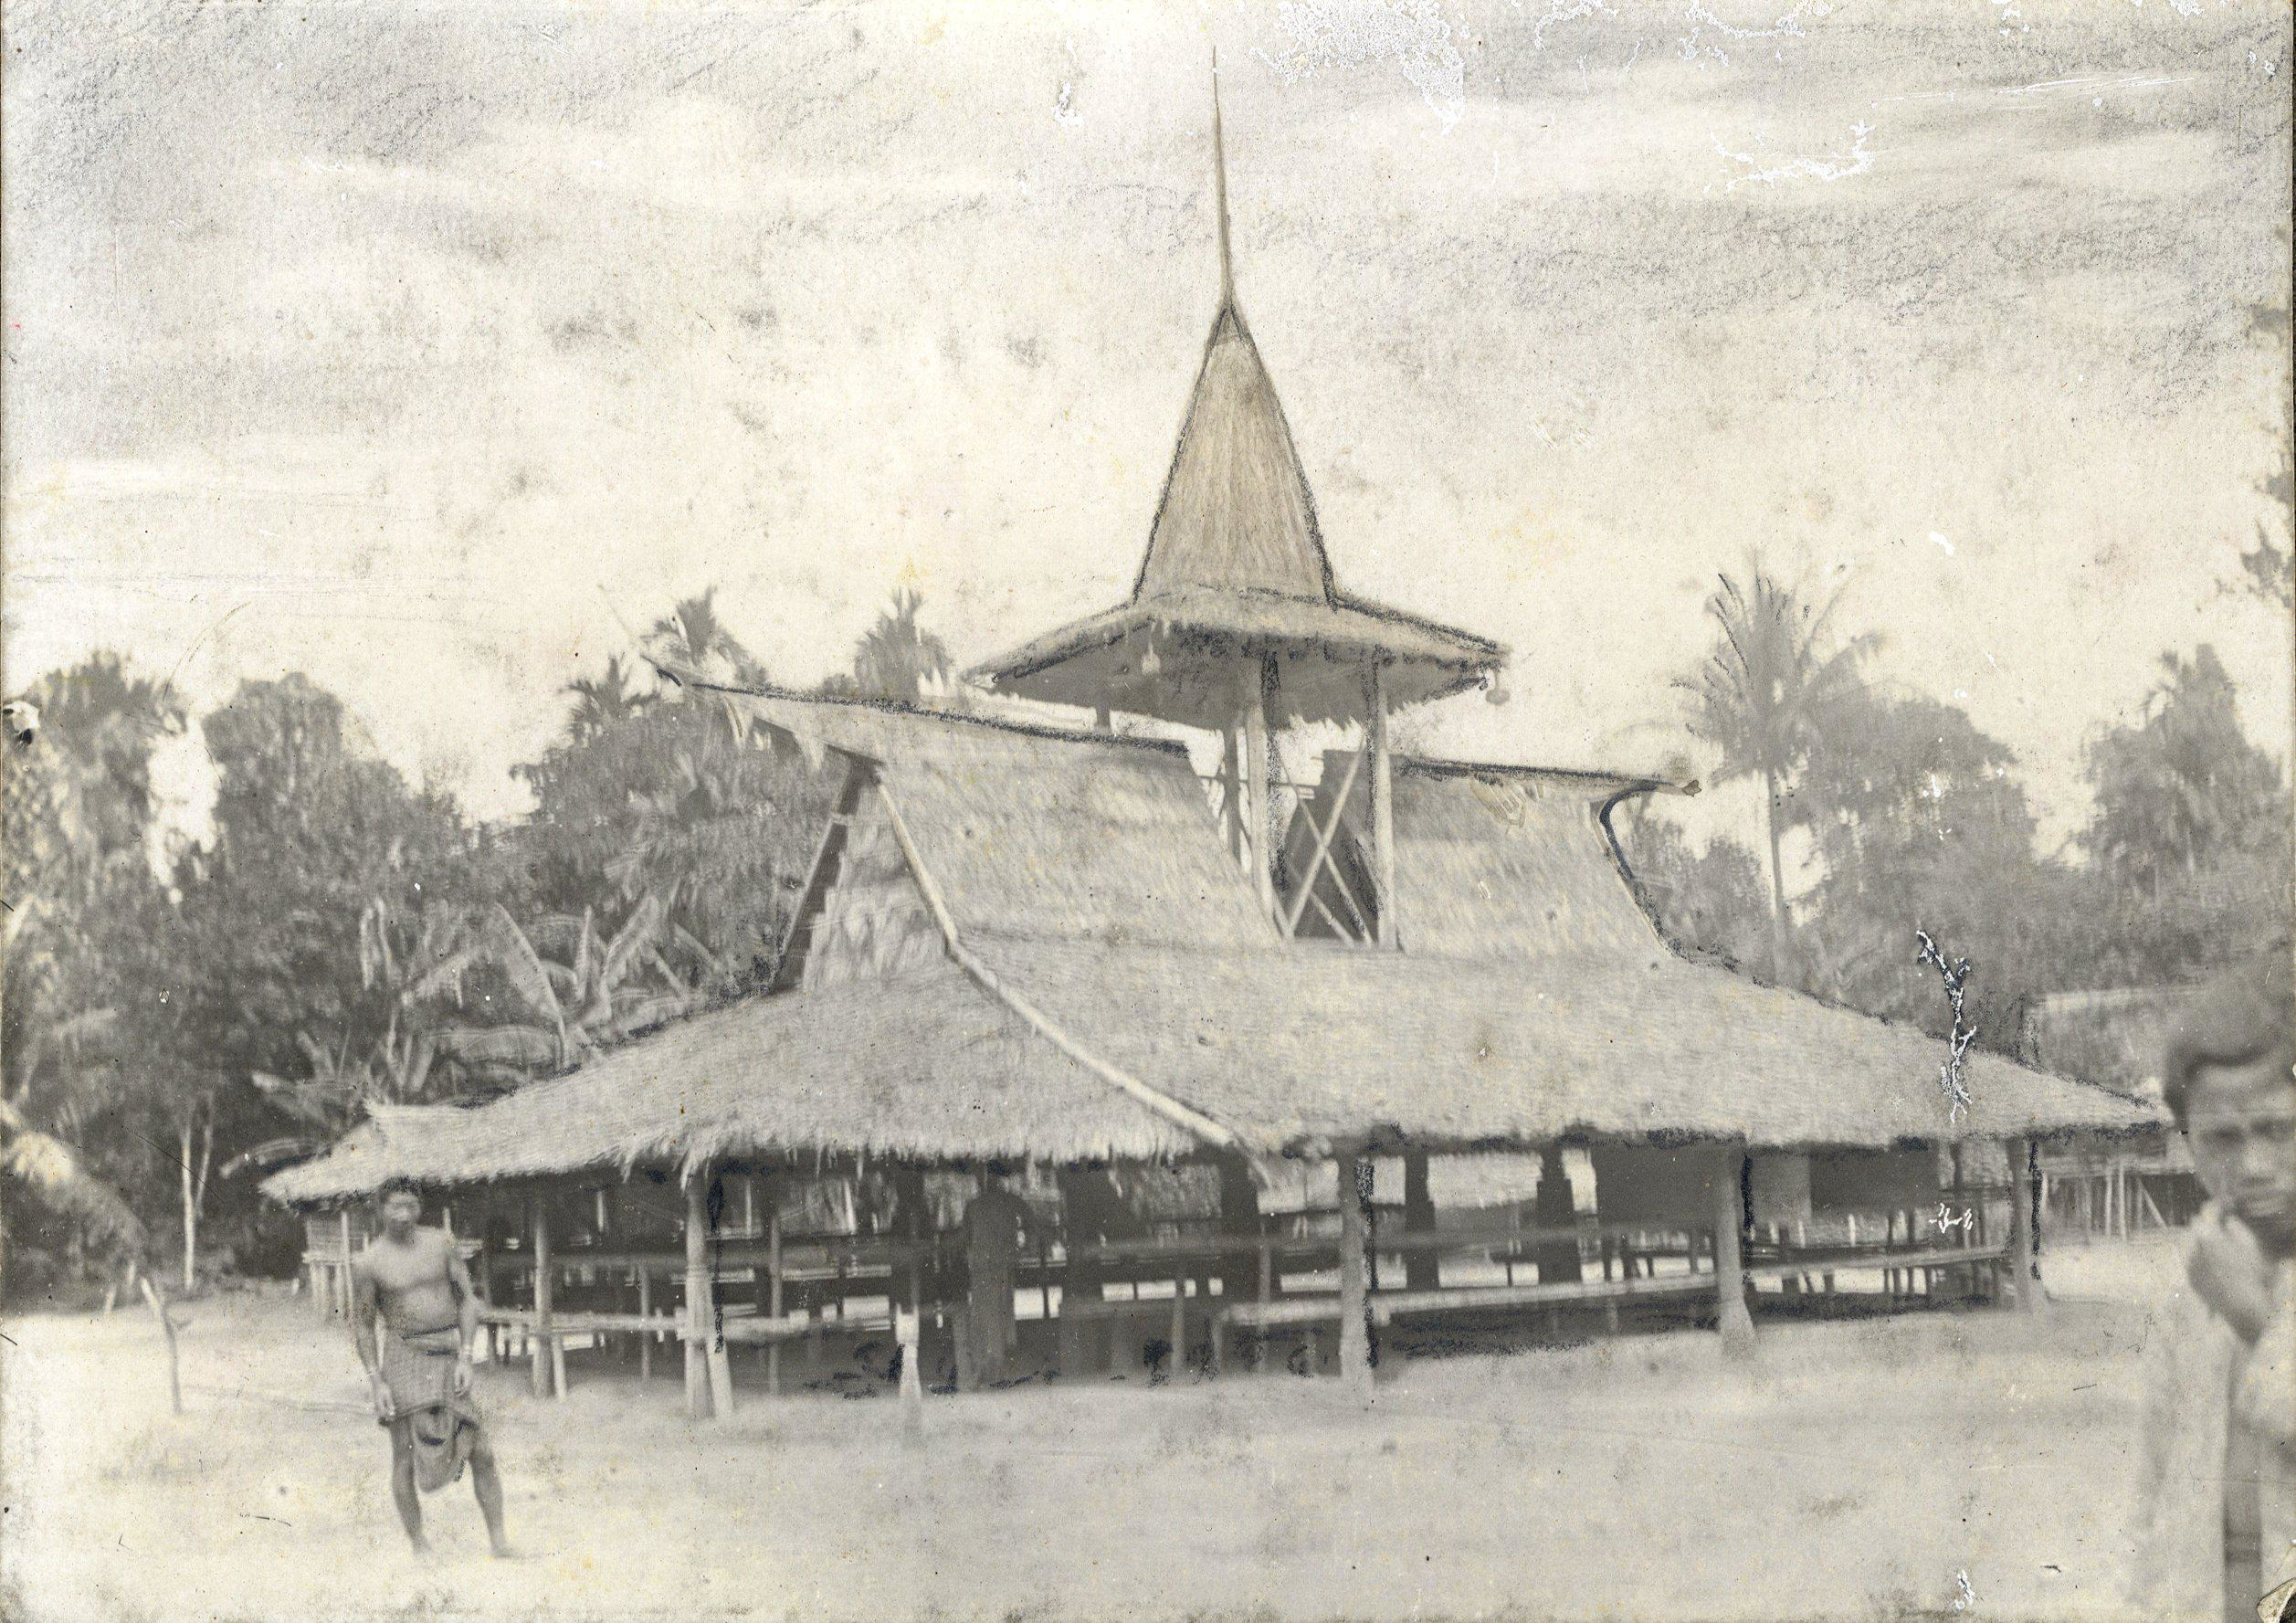
\includegraphics[width=1\linewidth]{figures/House.png}
    \caption{Photograph titled \textit{Gebouw te Toegoetils in Halmahera} (`Building of the Tugutils in Halmahera') from the KITLV archive (dated ca. 1910). [Public domain]}
    \label{fig:Tugutil_house}
\end{figure}

\section{The Modole language}
\label{sec:language}

\noindent Modole [mqo] (in some sources spelled Madole) is a Papuan language belonging to the North Halmahera language family. A map of the North Halmahera languages from 1908 can be found in Figure \ref{fig:NH_map}. Modole probably never had more than about 2,000 speakers -- the number of members of the group recorded throughout the early twentieth century until today.

Daily use of Modole is decreasing as speakers are shifting to North Moluccan Malay, the local variety of Malay and nowadays the major language of the North Moluccas  (see \cite{litamahuputty2012}). 
According to my Modole informant, Modole is still the main language in the villages of Kai, Pitago and Bailengi and children growing up there acquire Modole as L1. Modole speakers also have varying proficiency in Standard Indonesian and other local languages.

Modole is closely related to the other Core North Halmahera languages\footnote{This group includes all North Halmahera languages besides West Makian. I reconstruct their common ancestor as Proto-Core North Halmahera (\textsc{pcnh}).}, especially to those spoken on Halmahera proper (Mainland North Halmahera). Within the Core North Halmahera family, it subgroups with Tabaru and Pagu, which it closely resembles (see \citet{fortgens1928} for a description of Tabaru and \citet{peranginangin2018} for a description of Pagu). 
All Mainland North Halmahera languages are to a certain degree mutually intelligible and have been described as a continuum of dialects of the same language by \citet{voorhoeve1988}.
In 1910, G.J. Ellen reported that Tobelo was understood everywhere in the Kao ressort \citep[115]{ellen1910}. It is unclear whether this is due to mutual intelligibility of all languages in the area or because people were simply bilingual. 

According to \citet[189]{voorhoeve1988}, there is a northern and a southern dialect of Modole. The southern dialect has retained Proto-Core North Halmahera *s as /s/ while the Northern dialect has changed it to /h/.
In the 1980s, Northern Modole was spoken in the villages of Kai, Pitago, Bailengit, Soa-ma-etek, Parseba and Tuguis, while southern Modole was spoken in Soahukum, Tolabit-Torawat and Soasengaji (today called Sangaji Jaya).

Modole has borrowed a large number of lexical items from the local lingua franca Ternate and the wider lingua franca Indonesian. Other sources of loan words include Javanese (see Section \ref{subsec:folk_religion}) and European languages such as Portuguese and Dutch. Some loan words are indicated in the footnotes to the texts. 

Publications in and about Modole are scarce. The UZV missionary G.J. Ellen published a wordlist \citep{ellen1916b} with around 1,000 entries and the text collection edited in this book \citep{ellen1916}. In the late 19th century, Dutch colonial administrator K.F. Holle initiated the collection of wordlists for several Indonesian languages. The project was continued after his death and the wordlists are published in \citet{stokhof1980,stokhof1980a}. The Modole wordlist contains about 700 entries. The list is mentioned in the 1933 \textit{Jaarboek} of the \textit{Bataviaasch Genootschap van Kunsten en Wetenschappen} and it was likely collected between 1926 and 1932. The time and place of recording are unknown, as is the name of the recorder, but it is likely that Ellen was involved. The Holle wordlist deviates in some points from Ellen's wordlist.
In 1976, Yuiti Wada collected wordlists covering a total of 229 entries with two Modole speakers (published in \cite{wada1980}). In 1980, C.L. Voorhoeve recorded a wordlist and a short narrative in Modole. The recordings are now archived in PARADISEC.\footnote{See \url{https://catalog.paradisec.org.au/collections/CLV1/items/245} for the wordlist and \url{https://catalog.paradisec.org.au/collections/CLV1/items/260} for the continuation of the wordlist and the narrative (both accessed 4 October 2025).}
\citet{voorhoeve1988} includes some general remarks about the geographic and dialectal distribution of Modole. 
A Bible lesson was recorded in 2022 with a Modole speaker from Soamaetek for \citet{globalrecordings2023}.\footnote{I am grateful to Edward Kotynski for providing me with this information.} There is also a Modole version of the Jesus film \citep{jesusfilmprojectnd}. 
In 2024, the Indonesian government organization \textit{Badan Riset dan Inovasi Nasional} (BRIN) conducted linguistic research in the Modole village of Soamaetek, lead by Dyah Susilawati.\footnote{Personal communication with Dyah Susilawati, 12 January 2025}
As of September 2025, a Bible translation project is ongoing.
All these publications and projects are concerned with the northern dialect of Modole.

\begin{figure}
    \centering
    \includegraphics[width=.9\linewidth]{figures/Hueting1908.png}
    \caption{Approximate position of the North Halmahera languages in 1908, based on \citet{hueting1908}. [created by the author]}
    \label{fig:NH_map}
\end{figure}

\chapter{G.J. Ellen and the Halmahera mission of the Utrechtse Zendingsvereeniging}
\label{chap:Ellen}

Gerrit Jan Ellen (1876-1957)\footnote{see \url{https://webggc.oclc.org/cbs/DB=2.37/XMLPRS=Y/PPN?PPN=33831444X}, \url{https://hetutrechtsarchief.nl/collectie/AF6E16D8195046BB9CFADC700C5F24C9} (both accessed 4 October 2025)} was a missionary of the Utrechse Zendingsvereeniging (UZV; established 1859). This organization was part of the Protestant Dutch Reformed Church.
Information about Ellen's mission can be gathered from several publications: \textit{Handelingen der Utrechtsche Zendingsvereeniging}, \textit{Berichten van de Utrechtsche Zendingsvereeniging} as well as Ellen's (\citeyear{ellennda}) autobiographic report of his mission titled \textit{Uit mijn ervaring} (`From my experience'). For a history of the UZV mission in general see \citet{hueting1930}.
Ellen came to Halmahera in 1903 and worked there until he retired in 1938 \citep[188]{zendingsstudieraad1938}. 
For some years, he was accompanied by his wife N. Ellen-de Jong and (at least) two daughters born on Halmahera.
A picture of Ellen among his missionary colleagues is reproduced in Figure \ref{fig:conference}.\footnote{Link to the photograph: \url{http://hdl.handle.net/1887.1/item:827841} (accessed 4 October 2025)}

\begin{figure}
    \centering
    \includegraphics[width=1\linewidth]{figures/Zendelingenconferentie.jpg}
    \caption{Photograph titled \textit{Zendelingenconferentie te Tobelo in Halmahera} (`Missionary conference at Tobelo in Halmahera') from the KITLV archive (dated ca. 1910). The person identified as Ellen is circled. [Public domain]}
    \label{fig:conference}
\end{figure}

Within a few months of his arrival, he was allocated the Kao ressort. It covered the coast and interior north of Kao bay, that is the southern Tobelo settlements (Tobelo Boeng) and inland areas occupied by Pagu and Modole. In 1914, this ressort included 25 congregations with 2735 members \citep[136]{utrechtschezendingvereeniging1915}.

Ellen settled in the proximity of a coastal village called Pupupi and called the settlement Gamlaha (Ternate for `beautiful village') in 1907.\footnote{This is still the official name of the village as of 2025.}
The place is located in the Tobelo-Boeng speaking area. Ellen did not spend much time in the interior. Trips there were arduous and therefore seldom made (see \citet{ellennd}).

Ellen made first contact with the Modole in 1906 and some villages showed interest in becoming Christians \citep{ellen1906}.
In 1908, the mission had already advanced significantly among the Modole. There now was a guru called G. Tetalepta placed at Bailengit. His purview included people from the nearby villages Gogola ma lako (where all people had become Christians with the exception of four families) and Tomarate. Some of the inhabitants of Tomarate had moved to Bailengit and the rest was expected to follow them. This, Ellen explained, was necessary since a guru could only be placed in larger settlements \citep[158]{ellen1908}.
Both Gogola ma lako and Tomarate do not feature on modern maps, indicating that they were eventually abandoned.
The KITLV archive in Leiden hosts a photograph titled \textit{Leraar met zijn familie te Bailengit bij Kaoe in Halmahera} (`Teacher with his family at Bailengit near Kau in Halmahera'); see Figure \ref{fig:guru}.\footnote{Link to the photograph: \url{http://hdl.handle.net/1887.1/item:830771} (accessed 4 October 2025)} It is unknown if the photograph shows G. Tetalepta or a different guru.

\begin{figure}
    \centering
    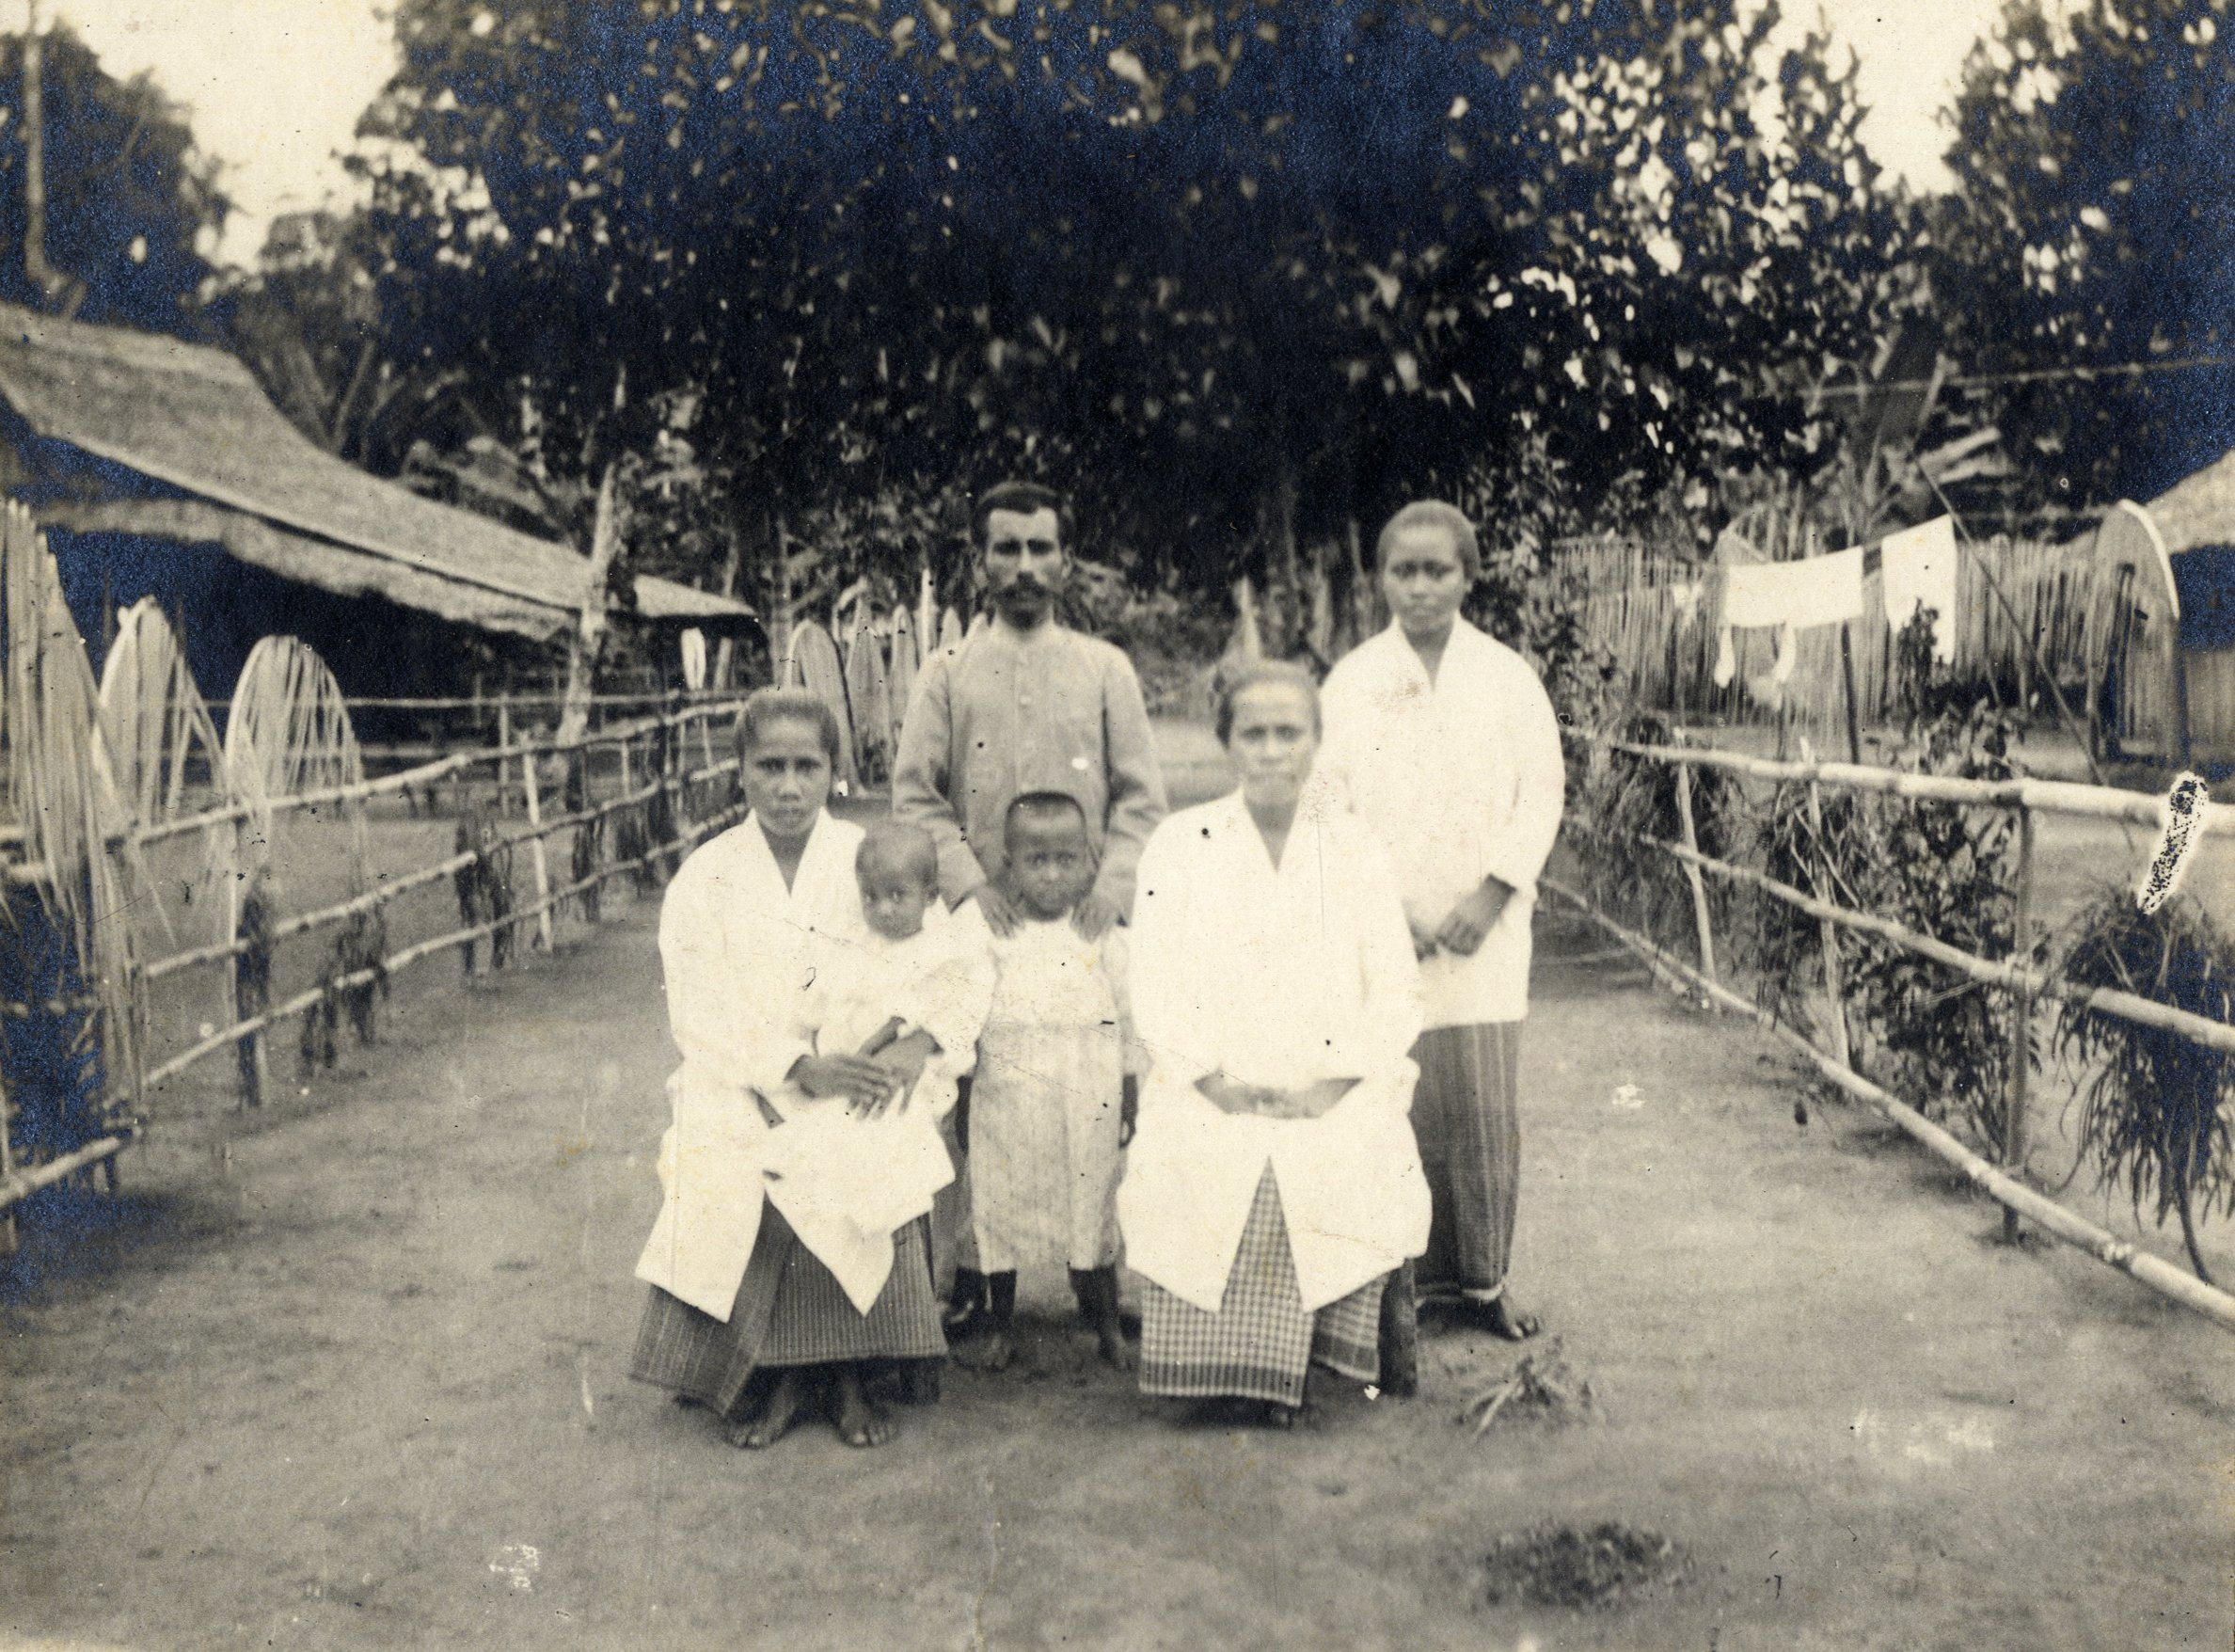
\includegraphics[width=1\linewidth]{figures/Guru_Bailengit.png}
    \caption{Photograph titled \textit{Leraar met zijn familie te Bailengit bij Kaoe in Halmahera} (`Teacher with his family at Bailengit near Kau in Halmahera') from the KITLV archive (dated ca. 1910). [Public domain]}
    \label{fig:guru}
\end{figure}

A guru by the name of P. Nanlohy was placed at Perseba. 
People in Toguis (Tuguis) were interested in Christianity while the inhabitants of Soamaetek still preferred to keep their native religion.
This had changed by 1918, when Ellen was able to report that almost everyone in Soamaetek was now baptized \citep{ellen1918}.

By 1908, Ellen had also visited the villages in the south Modole area: Soahukum, Tolabit and Soasengaji. People there were interested in Christianity but Ellen was unable to start work there since the villages had been partially abandoned due to recent unrest in the area \citep[159]{ellen1908}.
The people of Tolabit eventually converted in 1917 \citep[65]{leith1999}.
Today, most Modole are Christians.

As we can glean from his writings and published letters\footnote{These are letters he wrote to the council of the UZV published in the \textit{Berichten van de Utrechtsche Zendingsvereeniging}.}, Ellen's main goal in his work as a missionary was to enkindle a profound and personal Christian belief in the people of Halmahera. Further occupations of the UZV missionaries included the founding of schools (there were at least eight in Modole settlements by 1915) and the opening of income sources for the mission and the newly established congregations (for example coconut plantations). 
Ellen does not seem to have been particularly interested in linguistic and ethnological studies -- unlike some of his colleagues on Halmahera who published extensive dictionaries, grammatical descriptions and ethnological papers about the languages and people they encountered. 
Ellen preferred to discuss aspects of his mission in his writings. Information about the life of the people of Halmahera is only included whenever he laments the poor living standards. 
Information regarding Ellen's personal life is likewise absent. Even in his autobiographic work \textit{Uit mijn ervaring} \citep{ellennda} he does not discuss his life before he came to Halmahera or why he chose to become a missionary. I therefore know nothing about his educational background. Missionaries of the UZV went to a missionary seminar where, among other things, they studied Malay and sometimes also a local language relevant for their mission \citep{adriani1906}. Most likely, Ellen had no academic education in linguistics. 

\chapter{Provenance of the texts and this edition}
\label{chap:stories}

In this chapter, I attempt to shed some light on the provenance of the texts (\sectref{sec:provenance}). I also provide information on the structure and process of my edition of the texts (\sectref{sec:thisedition}).

\section{The provenance of the texts}
\label{sec:provenance}

As mentioned above, the provenance of the texts is unclear. 
Neither the story collection nor the accompanying wordlist \citep{ellen1916b} contains any information about who told the stories, and where and when they were recorded. To my knowledge, the Modole are now unfamiliar with the collection and preserve no memory of its recording.
Ellen first made contact with the Modole around 1906. He went on leave in July 1913 and stayed in the Netherlands until March 1915 (\cite{ellen1913, ellen1915}).
It is likely that he prepared and submitted the collection for publication during his stay in the Netherlands, which pinpoints their time of recording to between 1906 and 1913.

If Voorhoeve's (\citeyear{voorhoeve1988}) assertions are correct, the texts are recorded in the northern Modole dialect, since they reflect Proto-Core North Halmahera *s as /h/. This is even more likely since the northern Modole villages came under the influence of the mission at an earlier time than the southern villages (see Chapter \ref{chap:Ellen}). Potential places of collection are the villages of Perseba and Bailengit where gurus were placed at the collection time.

It is by no means certain that it was Ellen who wrote down the texts. Since Ellen did not spend much time in the Modole villages, they could well have been collected by one or more of the gurus who lived there permanently.\footnote{The archive of Ellen's UZV colleague J. Fortgens in Leiden hosts manuscripts in many different hands and some notebooks have the name of a guru on the cover.} 

I conducted no analysis of linguistic differences between the individual texts but it is notable that elements roughly meaning `then', used to structure the discourse, vary from text to text (see Table \ref{tab:discourse} for number of occurrences). 
The most frequent of these elements is \textit{geena('a) de} and it is the only one used in Texts \ref{chapter:text01} and \ref{chapter:text02}.  It is, however, absent from Texts \ref{chapter:text03} and (with one exception) Text \ref{chapter:text04}. These two texts use \textit{i'a} and \textit{ena} instead. The form \textit{geena'adau de} only occurs in Texts \ref{chapter:text05}, \ref{chapter:text06} and \ref{chapter:text07} and in Text \ref{chapter:text08} \textit{done} is used but does not occur in any other text.
This observation may be due to coincidence -- or it may point to different speakers, maybe even speakers from different villages. 

\begin{table}
    \caption{Discourse-structuring elements}
    \label{tab:discourse}
    \begin{tabularx}{.75\textwidth}{llllll}
        \lsptoprule
        &   \textit{geena'a de}&\textit{i'a}&  \textit{ena}&\textit{geena'adau de}&\textit{done}\\
        \midrule
        Text \ref{chapter:text01}&   7&--&  --&--  &--\\
        Text \ref{chapter:text02}&   8&--&  --&--  &--\\
        Text \ref{chapter:text03}&   --&1&  1&--  &--\\
        Text \ref{chapter:text04}&   1&8&  1&--  &--\\
        Text \ref{chapter:text05}&   2&--&  4&1  &--\\
        Text \ref{chapter:text06}&   4&3&  3&1&--\\
        Text \ref{chapter:text07}&   2&4&  --&4&--\\
        Text \ref{chapter:text08}&   3&1&  --&--  &2\\
        Text \ref{chapter:text09}&   1&--&  --&--  &--\\
        Text \ref{chapter:text10}&  --&--& --&--  &--\\ 
        \lspbottomrule
    \end{tabularx}
\end{table}

The background of the original editing and publication of the texts is as obscure as their collection. It is unknown whether Ellen translated the texts on his own or together with speakers of Modole. Ellen lived among Tobelo speakers and he was also acquainted with Pagu. With the help of the already published dictionaries and descriptions of other North Halmahera languages, he may have been able to produce reasonable translations on his own. There are several mistakes in the translation that point to this scenario. 

One mistake concerns the translation of a certain actor--undergoer combination. Modole shows a metathesis in the combination for a first person plural exclusive acting on a second person plural. Regularly, the form should be \textit{mi ni} and occurs as such in Pagu. Modole, on the other hand, has \textit{ni mi}. The Dutch translation mistook \textit{ni mi} for a second person plural acting on a first person plural exclusive in several cases.\footnote{Most of these cases are found in \textref{chapter:text04}. According to the Dutch translation, the ants ask the old people to search them for lice (\textsc{2pl>1pl.ex}). They then tell the old people to look up and throw lime into their eyes. This situation makes more sense if the ants search the old people who are seated with their back to the ants for lice (\textsc{1pl.ex>2pl}).} 
Ellen's translation should therefore always be checked with the original Modole text and the English translation provided by me.

\section{This edition}
\label{sec:thisedition}

For my analysis and translation of the texts, I used the FieldWorks Language Explorer (FLEx).\footnote{See \url{https://software.sil.org/fieldworks/} (accessed 4 October 2025)}
I copied the Modole text as well as the Dutch translation from an OCRed version of \citet{ellen1916} into FLEx and imported the available Modole wordlists (\cite{ellen1916b}, \cite{stokhof1980a}, \cite{wada1980}). I then compared the Dutch translation with the Modole text and the automatic matching of lexicon entries and word forms provided by FLEx. For unclear word forms or grammatical features, I checked dictionaries and descriptions of other North Halmahera languages. Some remaining questions were checked with a Modole speaker via an online messenger app. Unfortunately, it was not possible to check the complete translation with a Modole native speaker. 

Each of the texts is presented as follows in Chapters \ref{chapter:text01}--\ref{chapter:text10}. After a short introduction and summary of the text, I reproduce the Modole text in an adjusted spelling based on Indonesian orthography. This orthography is now used by Modole speakers, whereas not all of them are familiar with the Dutch-based orthography used by Ellen.\footnote{Notice that several grammatical items spelled separately by Ellen are nowadays conjoined with another word. It did not adopt this practise since there still is variation.} I have therefore given preference to the modern orthography here as well as in my morphemic analysis (see below) and the sketch grammar.
Deviations from the orthography used by Ellen are displayed in \tabref{tab:orthography}. 

\begin{table}
    \caption{Deviations between Ellen's and contemporary Modole orthography}
    \label{tab:orthography}
    \begin{tabularx}{.7\textwidth}{XXX}
        \lsptoprule
        \textsc{phoneme}&\textsc{ellen}&\textsc{contemporary}\\
        \midrule
        /j/& <dj> & <j>\\
        /c/&  <tj>& <c>\\
        /y/& <j> & <y>\\
        /ny/ & <nj> & <ny> \\
        \lspbottomrule
    \end{tabularx}
\end{table}

The letters <a> and <o> are often confused. This may be due to inconsistencies in transcription or typos introduced by the printers. I have not corrected any typos in order to preserve the original text but I have adjusted punctuation regarding direct speech. In the Modole text, colons and parentheses are often absent even where they occur in the Dutch translation. I inserted them so that now the Modole text and the Dutch as well as English translation correspond. I have not changed punctuation otherwise, even though it does not always feel adequate to the Modole language.\footnote{Commas and semicolons in the Modole text likely reflect Dutch conventions rather than breaks, for example.} 
Line breaks were introduced rather heuristically and are based both on Modole conjunctions such as \textit{de} `and', and punctuation.

Next is my English translation, which is based on the Modole text and differs in many points from Ellen's Dutch translation in the next section. See above for how I arrived at this translation.
The Dutch translation is faithful to the translation in \citet{ellen1916} with the exception of the addition of some missing colons and quotation marks. 

Next comes the interlinear glossed Modole text. The interlinear glossing is structured as follows:
The first line is the original Modole text and in most regards faithful to \citet{ellen1916}. Ellen's Dutch-based orthography is preserved here but missing colons and parentheses are added.
The second line presents my morphemic analysis (in modern orthography).
The third line contains the gloss of the morphemes found in the second line. In many cases, multiple glosses are possible. This is especially true for homographic morphemes like <ma> (`relational noun marker, `middle marker', `but', or `\textsc{3sgf>3nh}'), <o> (`noun marker', or incorrect spelling of the emphatic morpheme \textit{'o}) and <'a> (locative \textit{-o'a}, limitative \textit{-o'a}, or \textsc{itive} directional \textit{-i'a}). I was often left to guess and the glossing of these morphemes should hence always be taken with a grain of salt. Question marks indicate unclear glosses. Glosses are solely used as labels for often broader functions. For an analysis, the reader is pointed to the grammar sketch. 

The translation in the fourth line is more literal than the one presented above. I tried to imitate the original syntax as much as possible which in several cases leads to unidiomaticity in English. Most notably, I consistently translate the Modole directionals \textit{o'o} and \textit{iha} as `landward' and `seaward', respectively, in an attempt to reproduce this very prevalent feature of spatial orientation (see Section \ref{sec:directionals_locationals}). Punctuation follows the Modole original and hence is often inconsistent.
Uncertain translations are preceded by a question mark and alternative translations are discussed in the footnotes in the interlinear version of the texts.

\section{Overview of the texts}

\tabref{tab:texts} provides an overview of the texts included in this collection.

\begin{xltabular}{\textwidth}{lXr}
    \caption{The texts in this collection.} \label{tab:texts}\\

    \lsptoprule
        \textsc{text} & \textsc{title} & \textsc{words}\\
    \midrule
    \endfirsthead

    \multicolumn{3}{c}%
    {\tablename\ \thetable{} -- continued from previous page}\\
    \lsptoprule
        \textsc{text} & \textsc{title} & \textsc{words}\\
	\midrule
    \endhead

    \hline \multicolumn{3}{r}{{Continued on next page}}\\
    \endfoot

    
    \endlastfoot

    %\ref{chap02}&Clan history&&\textbf{2576}\\
		\ref{chapter:text01}&\textit{O lagudi ma howo’o wo djaga-djaga’a} - The guardian of the \textit{legundi} fruits&817\\
        \ref{chapter:text02}&\textit{O bibiti} - The \textit{bibiti} fish&699\\
        \ref{chapter:text03}&\textit{O Goda} - The \textit{goda} spirit&279\\
        \ref{chapter:text04}&\textit{O Gogunane} - The ants&658\\
        \ref{chapter:text05}&\textit{O lia’a de o dodoto} - The older and the younger brother&1161\\
        \ref{chapter:text06}&\textit{O uho} - The cuscus&1298\\
        \ref{chapter:text07}&\textit{O Biara} - The \textit{biara} plant&547\\
        \ref{chapter:text08}&\textit{Naga o njawa ja mididi jo puaha} - Two people who fasted&479\\
    %\ref{chap03}&Traditional stories&&\textbf{3531}\\
        \ref{chapter:text09}&\textit{O Lolabi mi tadi-tadi’a} - She is
stabbed by a kris&173\\
        \ref{chapter:text10}&\textit{Cumu cagulu} - Riddles&128\\
    \midrule    
        \textbf{total}&&\textbf{6239}\\
    \lspbottomrule
\end{xltabular}

\part{Sketch grammar}
    \chapter{Grammatical overview}\label{chapter:sketch}
    \section{Introduction}

In this chapter, I will outline the grammatical structure of Modole based on the texts in this collection. References to examples from the texts are in the format ``[A.1]'', where the letter refers to the text and the second digit refers to the respective line. Working with a corpus of such limited size has consequences for the grammatical description. Naturally, some phenomena will be unattested in the texts. Especially in the area of syntax the data is often inconclusive. Occasionally I asked a native speaker of Modole for judgments regarding certain structures but I refrained from incorporating any other Modole sources so that this sketch grammar would faithfully reflect the language of only the texts. My Modole informant found the texts comprehensible in general but struggled with the phasal polarity system, which seems to have changed a lot in the past 100 years.

Modole is structurally very similar to the closely related languages Tabaru and Pagu. I am of course influenced by descriptions of the latter two languages (especially by Perangin Angin's (\citeyear{peranginangin2018}) Pagu grammar). The identification of morpheme boundaries is partly based on descriptions of Pagu and Tabaru.
Nonetheless, I have tried as much as possible to describe the grammar of Modole in its own terms. Therefore, I only draw comparisons to other languages to improve understanding of rarely attested features. I also kept notes on diachronic issues to a minimum. The chapter is longer than what may be expected of a grammar sketch. Since this is the first extensive linguistic description of Modole, I discuss as many features as possible. 

Modole is a head-marking language. Predicates are morphologically more complex than arguments. The alignment is nominative--accusative in the sense that the single argument of a intransitive predicate is marked like the actor of an transitive verb. Predicates usually occur with actor and undergoer indices. Verbs are preceded by a number of morphemes that mostly mark changes in valency. Tense is not marked but there is a set of suffixes pertaining to the temporal domain, such as phasal polarity markers. Nominal modifiers (``adjectives'') have the form of intransitive verbs. Pronominals and indices distinguish clusivity and human vs. non-human referents. There is no nominal number or overt gender marking. Noun phrases as undergoer arguments are morphologically marked in certain contexts. Modole has an elaborate system of spatial notions along the three axes: \textsc{sea} vs. \textsc{land}, \textsc{up} vs. \textsc{down} and \textsc{ventive} vs. \textsc{itive}. Demonstratives are morphologically complex. The default word order is SOV but variations frequently occur.

\section{Orthography}

This section deals with orthography of Modole used in the texts as well as some basic phonology issues that can be gathered from the written text alone. Ellen used a Dutch-based orthography for Modole inspired by the works of his missionary colleague M.J. van Baarda for Galela \citep{vanbaarda1895, vanbaarda1904, vanbaarda1908}. Van Baarda was considered the best ``linguist'' by the other missionaries and they followed his standards (see \citet[11]{hueting1908}). This does not only concern the spelling of sounds but also which grammatical items were written independently or conjoined with another verb.\footnote{Van Baarda's theoretical considerations on this issue can be found in the works cited above.} 

\tabref{tab:consonant_phonemes} displays the graphemes and digraphs used to write consonants in Modole.\footnote{ The approximate pronunciations are based on evidence from other North Halmahera languages and modern recordings of Modole.} The modern orthography is put in parentheses where it deviates from Ellen's orthography. The graphemes <k> and <ny> are only found in loanwords (\textit{waktu} `time' (Malay, ultimately Arabic), \textit{nyawa} `person' (Malay), \textit{nyonyie} `sunrise' (Ternate)) and they are likely not phonemic. Proto-Core North Halmahera (\textsc{pcnh}) *r is reflected as /l/ or zero in most cases, but there are 52 roots attested in the stories that contain /r/. Most of these are loans from non-North Halmaheran languages. A root such as \textit{gorona}, which is likely native, could be a borrowing from another North Halmahera language (expected outcome in Modole is **gona\footnote{Two asterisks introduce an unattested form.}).

In (\ref{ex:minimalpairs_consonants}), I give at least one minimal pair for each grapheme/digraph to demonstrate that they represent phonemes. There is no minimal pair for /l/ vs. /r/ and the phonemic status of the latter is uncertain.

\begin{table}
    \caption{Consonant inventory of Modole}
    \label{tab:consonant_phonemes}
    \begin{tabularx}{\textwidth}{llllll}
    \lsptoprule
         &  \textsc{labial}&  \textsc{dental}/\textsc{alveolar}&  \textsc{palatal}&  \textsc{velar}& \textsc{glottal}\\
         \midrule
         \textsc{plosive}&  p b&  t d&  tj (c) dj (j)&  k g& ' \\
         \textsc{nasal}&  m&  n&   nj (ny)& ng\\
         \textsc{trill}&  &  r &  &  & \\
         \textsc{approximant}&  w&  l&  &  j (y)& h\\
         \lspbottomrule
    \end{tabularx}
\end{table}

\begin{exe}
    \ex 
    \label{ex:minimalpairs_consonants}
    \begin{xlist}
    \ex /b/ : /h/ : /l/ : /n/ \\
        \textit{abo} `foam' : \textit{aho} `dog' : \textit{alo} `beat sago' : \textit{ano} `a moment ago'
    \ex /p/ : /m/ \\
        \textit{hupu} `exit' : \textit{humu} `well'
    \ex /d/ : /g/ \\
        \textit{tadi} `stab' : \textit{tagi} `walk'
    \ex /t/ : /d/ : /y/ \\
        \textit{tai} `carry on the back' : \textit{dai} `\textsc{sea} locational' : \textit{yai}  `mother'
    \ex /c/ : /d/ \\
        \textit{cina} `China' : \textit{dina} `\textsc{land} locational'
        \ex /j/ : /n/ \\
        \textit{jaga{\textasciitilde}jaga} `guard' : \textit{naga} `\textsc{exist}'
    \ex /ng/ : /n/ \\
        \textit{ngamo} `angry' : \textit{namo} `chicken' 
    \ex /g/ : /r/ \\
        \textit{jaga{\textasciitilde}jaga} `guard' : \textit{jara} `horse'
    \ex /w/ : /'/ \\
        \textit{dawu} `sister in law' : \textit{da'u} `\textsc{up} locational' 
    \end{xlist}
\end{exe}

There seems to be a general rule that only one glottal stop occurs per word form (with a few exceptions). I do not know whether this is a synchronic phonological rule, or a mere orthographic convention. Some roots occur with and without a final syllable of the form /'V/, where V is identical to the preceding vowel. Examples are given in (\ref{ex:nmlz}). 

\begin{exe}
    \ex 
    \label{ex:nmlz}
    \begin{xlist}
    \ex \textit{wutu} `night' vs. once \textit{wutu'u} [B.\ref{ex:text2-23}]\footnote{or < \textit{wutu-u'u} `night-\textsc{dir.down}'}
    \ex \textit{ena'a} `areca' vs. once \textit{enaou} `chew betel' [B.\ref{ex:text2-46}]
    \ex \textit{la'o} `eye' vs. once \textit{la'o'o} [D.\ref{ex:text4-47}]
    \end{xlist}
\end{exe}

Ellen uses five graphemes to represent vowels: <a>, <e>, <i>, <o> and <u>. The minimal pairs given in (\ref{ex:minimalpairs_vowels}) show they represent phonemes. Some vowels are marked with a trema (e.g. <ä>, <ï>). Its function is unclear.

\begin{exe}
    \ex 
    \label{ex:minimalpairs_vowels}
    \begin{xlist}
    \ex /a/ : /u/ \\
        \textit{tana} `raise' : \textit{tanu} `modality marker'
    \ex /a/ : /e/ \\
        \textit{da'u} `\textsc{up} locational' : \textit{de'u} `mountain' 
    \ex /i/ : /o/ \\
        \textit{ai} `first person singular possessive' : \textit{ao} `take' 
    \end{xlist}
\end{exe}

There are several cases of roots where one vowel is spelled either <a> or <o> (e.g. \textit{gohapanata} vs. \textit{gahapanata} `kind of tree').
It is possible that /a/ and /o/ had phonetic realizations that were difficult to tell apart for the transcriber(s). Note that the Modole are called \textit{Madole} in most Dutch sources.\footnote{Alternatively, <a> and <o> may have been difficult to distinguish in handwriting by the printers.}

There is some evidence for a change of lexeme-final /u/ > /o/ if the following lexeme starts with /o/, e.g. \textit{no dapa'o o ngotili} [B.\ref{ex:text2-11}] instead of **dapa'u o.
The suffix \textit{-ou} is spelled <o> word-finally when the following word starts with an /o/; see \textit{hupu-o} in (\ref{ex:u>o}).

\begin{exe}
    \ex 
        \gll de na'o wo lamo'o'au, {ma moi} wo hupu-o o a'ele Itio \\
        \textsc{conn} \textsc{cond} 3\textsc{sg.m}.\textsc{a} big:\textsc{perf} once 3\textsc{sg.m}.\textsc{a} exit-\textsc{already} \textsc{nm} water Itio \\
        \trans ‘and when he had grown up, he once left the Itio river’ [A.\ref{ex:text1-16}] 
        \label{ex:u>o}
\end{exe}

The final vowel of a root is often lost when a suffix is attached. This seems to more frequently the case with directionals (see \sectref{sec:directionals_locationals}) than with other suffixes (see \sectref{sec:other_suffixes}).

\subsection{Onset mutation}\label{subsec:onset_mutation}

The Core North Halmahera languages share the feature of onset mutation. The initial consonant of a root is replaced with another consonant and vowel initial roots are prefixed with \textit{g-} or \textit{ng-}. Onset mutation has several functions and the most tangible one is deriving nouns from verbs. In the Modole texts, onset mutation seems to play a minor role and it is questionable whether it is productive. Attested mutation pairs are displayed in Table (\ref{tab:onset mutation}).

\begin{table}
    \caption{Onset mutation in Modole}
    \label{tab:onset mutation}
    \begin{tabularx}{.55\textwidth}{lcl}
        \lsptoprule
        \textsc{unmutated} & & \textsc{mutated} \\
        \midrule
        \textit{aha} `carry'&  :&\textit{gaha} `take'\\
        \textit{aho'o} `call'&  :&\textit{gaaho'o} `request'\\
        \textit{ai'i} `take out of'&  :&\textit{gai'i} `take'\\
        \textit{ali} `cry'&  :& \textit{gali} `cry'\\
        \textit{aliti} `exchange'&  :&\textit{ngaliti} `replace'\\
        \textit{oa} `end (n)'&  :&\textit{goa} `end (n)'\\
        \textit{oru} `row'&  :&\textit{ngoru} `row'\\
        \textit{parihi} `sweep'&  :&\textit{babarihi} `broom'\\
        \textit{tahe} `court (v)'&  :&\textit{dahe} `court (v)'\\
        \textit{tuulu} `follow'&  :&\textit{duulu} `after'\\
        \textit{umo} `throw'& :&\textit{gumo} `throw'\\
        \lspbottomrule
    \end{tabularx}
\end{table}


\subsection{Reduplication}\label{subsec:redupl}

Reduplication is a common morphological process in Modole. There are three attested reduplication patterns: total reduplication, partial reduplication of the first two syllables of a root ((C\textsubscript{1})V\textsubscript{1}(C\textsubscript{2})V\textsubscript{2}{\til}) and partial reduplication of only the first syllable (C\textsubscript{1}V\textsubscript{1}{\til}). 
Only bisyllabic roots can undergo total reduplication. The distribution of the other two patterns is not entirely clear to me. 

The same is true for the mapping of functions onto patterns. 
Reduplication of only the first syllable commonly derives noun from verbs, e.g. \textit{le{\til}letongo} `mask' (from \textit{letongo} `shine') or \textit{ba{\til}barihi} `broom' (from \textit{parihi} `sweep').

Reduplication can have an itensifying function as in (\ref{ex:redpl_intens}).\footnote{Notice that the \textsc{down} directional \textit{u'u} has the same function.}
In other examples, reduplication yields an imperfective reading (eg. durative, frequentative or habitual). For example, the reduplication of \textit{gogele} `sit' means `stay' (compare [E.\ref{ex:text5-78}] vs. [G.\ref{ex:text7-30}]). In (\ref{ex:total_rdpl}), the reduplicated form \textit{hungi-hungi} `search for game with dogs' refers to someones occupation.
Reduplicated forms with imperfective reading frequently occur in relative clauses (see \sectref{subsec:relative_clause}).

\begin{exe}
    \ex
    \begin{xlist}
    \ex 
    \gll mi huhu ho mi punu{\til}punuhu'u\\
    3\textsc{sg.f}>3\textsc{sg.m}	breast	thus	3\textsc{sg.f}>3\textsc{sg.m}	\textsc{rdpl}{\textasciitilde}satisfied:\textsc{dir}.\textsc{down}\\
\glt `she nursed him so that he was completely satisfied' [G.\ref{ex:text7-50}]\label{ex:redpl_intens}
    \ex 
        \gll wo hungi{\til}hungi \\
        3\textsc{sg.m}.\textsc{a} search.for.game.with.dogs \\
        \trans `he was a hunter' [C.\ref{ex:text3-3}]
        \label{ex:total_rdpl}
    \end{xlist}
\end{exe}

Prefixes are reduplicated as well, for example the applicative \textit{dV-} (\ref{ex:rdpl_dV}).\footnote{Notably, causative \textit{hi-} is never reduplicated}.

\begin{exe}
    \ex 
    \gll abei'a dauwe-ngo'o mi ma hi-du{\textasciitilde}du-tuumo \\
     well	\textsc{loc}.\textsc{down}-\textsc{n:dir.sea}	1\textsc{pl}.\textsc{ex}.\textsc{a}	\textsc{mid}	\textsc{caus-rdpl}{\textasciitilde}\textsc{appl}-?follow.with.raft\\
    \trans `come, [let]'s (ex.) ?follow the river with a raft down to the sea' [B.\ref{ex:text2-68}]
    \label{ex:rdpl_dV}
\end{exe}

Since I am unable to match patterns to functions I gloss reduplication as \textsc{rdpl}. If a root only occurs in reduplicated form, as is the case with \textit{hungi-hungi}, the whole form is glossed with the lexical meaning once. In the glosses texts, the two partial reduplication patterns are indicated as \textit{CV} and \textit{(C)V(C)V}.

Occasionally repetition of the whole verb form including indices occurs (\ref{ex:redpl_VP}). The meaning seems to be durative/frequentative.

\begin{exe}
    \ex 
    \gll gena-'a-de yo tagi-yo tagi\\
     \textsc{dist}:\textsc{pro}.3\textsc{nh}-\textsc{locv}-\textsc{conn}	3\textsc{hpl}.\textsc{a}	go-3\textsc{hpl}.\textsc{a}	go\\
    \trans `then they walked on' [H.\ref{ex:text8-24}]
    \label{ex:redpl_VP}
\end{exe}


\section{Parts of speech}

Verbs and nouns can be distinguished in Modole based on the grammatical elements they co-occur with. Verbs occur with indices while nouns are preceded by noun markers or possessives. Many roots can function as both verbs and nouns. There are two means of nominalization (onset mutation and reduplication). Nominalized stems sometimes occur with indices as well. 

%arguments and predicates
Most predicates are verbs. Types of predicates belonging to the realm of non-verbal predication in many languages (e.g. equative clauses) are treated like intransitive verbs and take verbal morphology.
Arguments are personal pronouns, demonstratives or nouns.  

%predication & attribution
A distinction between predication and attribution is seldom made and there is no adjective class. Nominal modifiers usually come in the form of intransitive verbs. The same is true for some kinds of adverbials. 

%affixes
As mentioned in the orthography section above, Ellen used an orthography devised by van Baarda for Galela. In this orthography, several grammatical elements are written separately that would now be considered affixes or clitics. For example, the Modole middle marker \textit{ma} is written separately while the causative marker \textit{si-} is attached to the following verb. Since I cannot say anything about the phonological status of these elements, I will only call elements affixes if they are written conjoined with another lexeme.

\section{Personal pronouns and indices}

Person (and in most cases number as well) is obligatorily expressed on verbs in the form of indices.\footnote{That is bound, referential person forms that express an referent without the obligatory overt expression of these referents by other linguistic means; see \citet{haspelmath2013}.} Optionally, a free personal pronoun can be added as well. Both personal pronouns and indices are written independently in the texts. There are just a few examples where an index is merged with a verb, e.g. \textit{j'odomo} `they eat' [A.\ref{ex:text1-34}].

Third person personal pronouns and indices show a gender distinction between human and non-human referents and, within the human category, also between singular feminine and masculine referents.
For human referents, there are separate personal pronouns and indices expressing feminine singular, masculine singular, and plural, while for non-human referents only one set of personal pronouns and indices exists, without number or gender distinctions (see \tabref{tab:gender_pp_ind}).\footnote{The distinction between plural human and non-human actors is not found in actor-undergoer combinations, see \sectref{subsubsec:pronouns_indices-indices-actor_undergoer}.}

\begin{table}
    \caption{Gender distinction in third person personal pronouns, actor indices and undergoer indices}
    \label{tab:gender_pp_ind}
    \begin{tabularx}{.55\textwidth}{Xll}
        \lsptoprule
         &  +\textsc{human}& --\textsc{human}\\
         \midrule 
         \textsc{feminine}&  \textit{muna}, \textit{mo}, \textit{mi}& \multirow{3}{*}{\textit{ena, i, a}}\\
         \textsc{masculine}&  \textit{una, wo, wi}& \\
         \textsc{plural}&  \textit{ona, yo, 'i}& \\
         \lspbottomrule
    \end{tabularx}
\end{table}

\subsection{Personal pronouns}

The personal pronouns of Modole are displayed in \tabref{tab:pronouns}. They function as expressions of actor (\ref{ex:PP_actor}), undergoer (\ref{ex:PP_undergoer}), and possessor roles (\ref{ex:PP_possessor}), and as predicates (\ref{ex: PP_predicate}). They can co-occur with indices. 

\begin{table}
    \caption{Modole independent pronouns}
    \label{tab:pronouns}
    \begin{tabularx}{.25\textwidth}{ll}
         \lsptoprule
         1\textsc{sg}& \textit{ngoi}\\
         2\textsc{sg}& \textit{ngona}\\
         3\textsc{sg.f}& \textit{muna}\\
         3\textsc{sg.m}& \textit{una}\\
         1\textsc{pl.in}& \textit{ngone}\\
         1\textsc{pl.ex}& \textit{ngomi}\\
         2\textsc{pl}& \textit{ngini}\\
         3\textsc{hpl}& \textit{ona}\\
         3\textsc{nh}& \textit{ena}\\
         \lspbottomrule 
    \end{tabularx}
\end{table}

\begin{exe}
    \ex 
    \begin{xlist}
    \ex 
        \gll de ngoi to hila-u \\
        \textsc{conn} \textsc{pro}.1\textsc{sg} 1\textsc{sg}.\textsc{a} first-\textsc{already} \\
        \trans `then I will [go] forward' [A.\ref{ex:text1-14}]
        \label{ex:PP_actor}
    \ex 
        \gll o jara i na tulu ngone \\
        \textsc{nm} horse 3\textsc{nh}.\textsc{a} 1\textsc{pl.in}.\textsc{u} transport \textsc{pro}.1\textsc{pl.in} \\
        \trans `a horse will pick us (in.) up' [H.\ref{ex:text8-32}]
        \label{ex:PP_undergoer}
    \ex 
        \gll neena to ngona ani lagudi ma howo'o? \\
        \textsc{prox}:\textsc{pro}.3\textsc{nh} \textsc{poss.hum} \textsc{pro}.2\textsc{sg} 2\textsc{sg}.\textsc{poss} legundi \textsc{rnm} fruit \\
        \trans `are these your (sg.) \textit{legundi} fruits?' [A.\ref{ex:text1-94}]
        \label{ex:PP_possessor}
    \ex 
\gll o'ia-no ngini ma nyawa? \\
what-\textsc{dir.ven} \textsc{pro}.2\textsc{pl} \textsc{rnm} person \\
\trans `where have you (pl.) [come from] here?' [F.\ref{ex:text6-150}]
\label{ex: PP_predicate}
    \end{xlist}
\end{exe}

The third person non-human personal pronoun \textit{ena} has additional functions but the full scope is not clear to me. In the example in (\ref{ex:ena_cons}) it seems to separate constituents in a clause, signaling that \textit{do'a} modifies \textit{manga ngio'a} `their place' and not \textit{ma wutu tumudingi} `seven nights'.

\begin{exe}
    \ex
        \gll ma wutu tumudingi ena do'a manga ngi-o'a yo arababu \\
        \textsc{rnm} night seven \textsc{pro}.3\textsc{nh} \textsc{locv} 3\textsc{hpl}.\textsc{poss} place-\textsc{locv} 3\textsc{hpl}.\textsc{a} native.violin \\
        \trans `[after] seven days there at their place they were playing the violin' [C.\ref{ex:text3-38}]
        \label{ex:ena_cons}
\end{exe}

\subsection{Predicate indices}

Actor\footnote{an agent-type role} and undergoer\footnote{a patient-type role} indices are the only obligatory verbal inflection.\footnote{See \citet[80]{naess2007} for an overview on the terms `actor' and `undergoer'.} They precede the verb in the ordering actor--undergoer.

\subsubsection{Actor indices}

The actor indices are displayed in \tabref{tab:actor_indices}.
The label \textit{actor} may be misleading since the referent of the actor index does not always have the semantic role of an agent. It can also be a theme (in locational clauses) or experiencer.\footnote{I chose the labels \textit{actor} and \textit{undergoer} over \textit{subject} and \textit{object} since the data does not allow for subjecthood tests.}

\begin{table}
    \caption{Actor indices}
    \label{tab:actor_indices}
    \begin{tabularx}{.25\textwidth}{ll} 
    \lsptoprule
        1\textsc{sg} & \textit{to} \\ 
        2\textsc{sg} & \textit{no} \\ 
        3\textsc{sg.f} & \textit{mo (mu)}\\ 
        3\textsc{\textsc{sg.m}} & \textit{wo (u)}\\ 
        1\textsc{pl.in} & \textit{po} \\ 
        1\textsc{pl.ex} & \textit{mio (mi)}\\ 
        2\textsc{pl} & \textit{nio (ni)}\\ 
        3\textsc{hpl} & \textit{yo} \\ 
        3\textsc{nh} & \textit{i} \\
    \lspbottomrule 
    \end{tabularx}
\end{table}

The first person plural exclusive and the second person plural indices occur without the final /o/ as \textit{mi} and \textit{ni}, respectively, before the middle marker \textit{ma}: \textit{mi mao'o} `we (ex.) defecate' [B.\ref{ex:text2-64}], \textit{ni ma guguule} `you (pl.) play' [F.\ref{ex:text6-82}] (see \sectref{subsec:middle} on the middle marker).
The third person singular feminine and masculine indices have the allomorphs \textit{mu} and \textit{u}, respectively, before the middle marker \textit{ma}: \textit{de ami utu mu ma bilinganaau} `and she spread out her hair' [B.\ref{ex:text2-53}], \textit{de una u ma iuno'a} `and he hid himself' [E.\ref{ex:text5-113}].

The third person non-human actor index \textit{i} is sometimes used for third person plural human referents if they are continued actors (\ref{ex:continued_actor}).

\begin{exe}
    \ex 
        \gll de yo iha de i lio-o de i temo \\
        \textsc{conn} 3\textsc{hpl}.\textsc{a} \textsc{dir.land} \textsc{conn} 3\textsc{nh}.\textsc{a} return-\textsc{already} \textsc{conn} 3\textsc{nh}.\textsc{a} say \\
        \trans `and they went landwards and they returned and they said' [E.\ref{ex:text5-41}]
    \label{ex:continued_actor}
\end{exe}

Some actor indices change their form when they are combined with certain undergoer indices. This is discussed in \sectref{subsubsec:pronouns_indices-indices-actor_undergoer}.

\subsubsection{Undergoer indices}

The forms of the isolated undergoer indices are given in \tabref{tab:undergoer_indices}. The undergoer indices comprise more semantic roles than Patient, including Recipient and Beneficiary. In terms of grammatical roles, they mark both direct and indirect objects (see \sectref{subsec:ditranstive_clauses}).

\begin{table}
    \caption{Undergoer indices}
    \label{tab:undergoer_indices}
    \begin{tabularx}{.2\textwidth}{ll} 
        \lsptoprule
        1\textsc{sg} & \textit{i} \\ 
        2\textsc{sg}& \textit{ni}\\ 
        3\textsc{sg.f}& \textit{mi}\\ 
        3\textsc{sg.m}& \textit{wi}\\ 
        1\textsc{pl.in} & \textit{na}\\ 
        1\textsc{pl.ex}& \textit{mi}\\ 
        2\textsc{pl}& \textit{ni}\\ 
        3\textsc{hpl}& \textit{'i}\\ 
        3\textsc{nh}& \textit{a}\\ 
        \lspbottomrule
    \end{tabularx}
\end{table}

Undergoer indices (with the exception of the third person plural human and the third person non-human) often occur without actor indices. This is discussed in the next section.

\subsubsection{Actor-undergoer combinations}\label{subsubsec:pronouns_indices-indices-actor_undergoer}

A verb can occur with both actor and undergoer indices. The undergoer either expresses the patient of a transitive verb or the (human) recipient or beneficiary of a ditransitive verb.
In some combinations, one of the two indices has a form different from the index in isolation, and sometimes the two indices have fused. 
The third person plural human actor index \textit{yo} only occurs in combinations if the undergoer is third person plural human as well \textit{yo 'i}. Otherwise, third person plural human actors are marked like third person non-human actors. However, the actor index only surfaces in combinations with first person plural inclusive (\textit{i na}) and third person non-human undergoers (\textit{ya}).

\tabref{tab:actor-undergoer-indices} shows the attested combinations of actor and undergoer indices.
The label \textsc{mid} indicates that the middle marker \textit{ma} (see Section \ref{subsec:middle}) is used instead of an undergoer index. En-dashes symbolize unattested combinations.


\begin{table}
    \caption{Attested actor-undergoer combinations}
    \label{tab:actor-undergoer-indices}
    \fittable{
    \begin{tabular}{llllllllll}
        \lsptoprule
        &  1\textsc{sg}.\textsc{u}&  \textsc{2sg.u}&  3\textsc{sg.f}.\textsc{u}&  3\textsc{sg.m}.\textsc{u}&  1\textsc{pl.in}.\textsc{u}&  1\textsc{pl.ex}.\textsc{u}&  2\textsc{pl}.\textsc{u}&  3\textsc{hpl}.\textsc{u}& 3\textsc{nh}.\textsc{u}\\ \midrule
        1\textsc{sg}.\textsc{a}&  \textsc{mid}&  \textit{to ni} &  \textit{to mi}&  \textit{to wi}&  \textsc{mid}&  \textsc{mid}&  \textit{ti ni}&  \textit{to 'i}& \textit{ta}\\ 
        2\textsc{sg}.\textsc{a}&  \textit{no i}/\textit{ni}&  \textsc{mid}&  \textit{no mi}&  \textit{no wi}&  \textit{no na}& \textit{ni mi} &  \textsc{mid}&  \textit{no 'i}& \textit{na}\\ 
        3\textsc{sg.f}.\textsc{a}&  \textit{mo i}&  --&  --& \textit{mi} &  --&  \textit{mi}&  --&  \textit{mo'i}& \textit{ma}\\ 
        3\textsc{sg.m}.\textsc{a}&  --&  --&  \textit{wi}&  \textit{wi}&  --&  \textit{wi}&  --&  \textit{wo 'i}& \textit{wa}\\ 
        1\textsc{pl.in}.\textsc{a}&  \textsc{mid}&  --&  --&  \textit{po wi}&  \textsc{mid}&  \textsc{mid}&  \textsc{mid}&  \textit{po 'i}& \textit{pa}\\ 
        1\textsc{pl.ex}.\textsc{a}&  \textsc{mid}&  --&  --&  --&  \textsc{mid}&  \textsc{mid}&  \textit{ni mi}&  --& \textit{mia}\\ 
        2\textsc{pl}.\textsc{a}&  \textit{ni}&  \textsc{mid}&  \textit{ni mi}&  --&  --&  \textit{ni mi}&  \textsc{mid}&  \textit{nio 'i}& \textit{nia}\\ 
        3\textsc{hpl}.\textsc{a}&  --&  --&  --&  --&  --&  --&  --&  \textit{yo 'i}& --\\ 
        3\textsc{nh}.\textsc{a}&  --&  \textit{ni}&  \textit{mi}&  \textit{wi}&  \textit{i na}&  \textit{mi}&  \textit{ni}&  --& \textit{ya}\\ 
        \lspbottomrule
    \end{tabular}
    }
\end{table}

As mentioned above, the third person non-human actor index \textit{i} surfaces in combination with first person plural inclusive undergoers (\textit{i na}, (\ref{ex:3nhA_1pl.inU}))\footnote{The same exception is found in Tabaru \citep[262]{holton2008}.} and third person non-human undergoers (\textit{ya} < *i-a, (\ref{ex:3nhA_3nhU})). The same form \textit{ya} is used for third person plural human actors acting on third person non-human undergoers. There is no example of a third person non-human actor acting on a third person plural human undergoer.

\begin{exe}
    \ex 
    \begin{xlist}
    \ex
        \gll o jara i na tulu ngone \\
        \textsc{nm} horse 3\textsc{nh}.\textsc{a} 1\textsc{pl.in}.\textsc{u} transport \textsc{pro}.1\textsc{pl.in} \\
        \trans `a horse will pick us (in.) up' [H.\ref{ex:text8-32}]
    \label{ex:3nhA_1pl.inU}
    \ex 
        \gll ai pihanga o gogunane ya odomo \\
        1\textsc{sg}.\textsc{poss} banana \textsc{nm} ant 3\textsc{nh}>3\textsc{nh} eat \\
        \trans `my bananas [were] eaten by ants' [D.\ref{ex:text4-13}]
    \label{ex:3nhA_3nhU}
    \end{xlist}
\end{exe}

For the second person singular and plural the same undergoer index \textit{ni} is used. However, number is disambiguated by a preceding singular actor index which ends in /o/ if the undergoer is a second person \textit{singular} (e.g. \textit{to ni} `1\textsc{sg}>2\textsc{sg}', see (\ref{ex:toni})) and in /i/ if the undergoer is a second person \textit{plural} (e.g. \textit{ti ni} `1\textsc{sg}>2\textsc{pl}', see (\ref{ex:tini})).

\begin{exe}
    \ex 
    \begin{xlist}
    \ex
        \gll to ni modoa-'a \\
        1\textsc{sg}.\textsc{a} 2\textsc{sg.u} marry-\textsc{lim} \\
        \trans `I will marry you (sg.)' [B.\ref{ex:text2-74}]
        \label{ex:toni}
    \ex 
        \gll ti ni modo'a \\
        1\textsc{sg.a} 2\textsc{pl.u} marry \\
        \trans `I will marry you (pl.)' [D.\ref{ex:text4-83}]
        \label{ex:tini}
    \end{xlist}
\end{exe}

Likewise, third person singular feminine and the first person plural exclusive undergoer referents are both expressed by \textit{mi}. They are only disambiguated with a second person singular actor: \textit{no mi} `2\textsc{sg}>3\textsc{sg.f}' (\ref{ex:nomi}) vs. \textit{ni mi} `2\textsc{sg}>1\textsc{pl.ex}' (\ref{ex:nimi}).

\begin{exe}
    \ex 
    \begin{xlist}
    \ex 
        \gll ua no mi hi-gu-mada \\
        \textsc{proh} 2\textsc{sg.a} 3\textsc{sgf.u} \textsc{caus}-?-abandon \\
        \trans `don't abandon her' [C.\ref{ex:text3-31}]
        \label{ex:nomi}
    \ex 
        \gll uwa ni mi poha \\
        \textsc{proh} 2\textsc{sg.a} 1\textsc{pl.ex.u} hit \\
        \trans `don't strike us (ex.)' [D.\ref{ex:text4-10}]
        \label{ex:nimi}
    \end{xlist}
\end{exe}

The isolated third person singular feminine undergoer index is \textit{mi} (\ref{ex:3sgf.U}) but \textit{mi} also expresses a third person singular feminine actor acting on a third person singular masculine undergoer (\ref{ex:3sgf>3sgm}), or first person plural exclusive undegoer (\ref{ex:3sgf>1pl.ex}). 

\begin{exe}
    \ex 
    \begin{xlist}
    \ex 
        \gll o goda mi haiti-au \\
        \textsc{nm} k.o.spirit 3\textsc{sg.f}.\textsc{u} seize-\textsc{already} \\
        \trans `the \textit{goda} spirit seized her' [C.\ref{ex:text3-29}]
        \label{ex:3sgf.U}
    \ex
        \gll de mi ma'e i tiai \\
        \textsc{conn} 3\textsc{sg.f}>3\textsc{sg.m} see 3\textsc{nh}.\textsc{a} straight \\
        \trans `and she saw him well' [B.\ref{ex:text2-35}]
        \label{ex:3sgf>3sgm}
    \ex 
        \gll nia eha muna dai mu o te{\til}teng-o'a mi hi-dupuhu-ie \\
        \textsc{2pl.poss} mother \textsc{pro.3sgf} \textsc{loc.sea} \textsc{3sgf.a} \textsc{emph} \textsc{rdpl}{\til}alone-\textsc{lim} \textsc{3sgf>1pl.ex} \textsc{caus-}follow\textsc{-dir.up} \\
        \trans `your (pl.) mother is by the sea, she is alone, [and] she will follow us (ex.) up' [F.\ref{ex:text6-169}]
        \label{ex:3sgf>1pl.ex}
    \end{xlist} 
\end{exe}

Likewise, \textit{wi} expresses an isolated third person singular masculine undergoer (\ref{ex:3sgm.U}) but also a third person singular masculine actor acting on a third person singular feminine undergoer (\ref{ex:3sgm>3sgf}), a third person singular masculine undergoer (\ref{ex:3sgm>3sgm}) or a first person plural exclusive undergoer (\ref{ex:3sgm>1pl.excl}).

\begin{exe}
    \ex 
    \begin{xlist}
    \ex %3sgm.U
        \gll ami pahita'a wi da-haba'a una-'a \\
        3\textsc{sg.f}.\textsc{poss} mask 3\textsc{sg.m}.\textsc{u} \textsc{appl-}touch.by.accident \textsc{pro}.3\textsc{sg.m}-\textsc{dir.itv} \\
        \trans `her mask hit him by accident' [E.\ref{ex:text5-87}]
        \label{ex:3sgm.U}
    \ex %3sgm>3sgf
        \gll wi ma'e-o o bere'i mo moi \\
        3\textsc{sg.m}>3\textsc{sg.f} meet-\textsc{already} \textsc{nm} old.person 3\textsc{sg.f}.\textsc{a} one \\
        \trans `he met an old woman' [A.\ref{ex:text1-17}]
        \label{ex:3sgm>3sgf}
    \ex %3sgm>3sgm
        \gll 'o-ne ma lia'a wi tomang-ou ma dodoto \\
        \textsc{emph}-\textsc{prox} \textsc{rnm} older.sibling 3\textsc{sg.m}>3\textsc{sg.m} wake.up-\textsc{already} \textsc{rnm} younger.sibling \\
        \trans `so the older brother woke up the younger one' [H.\ref{ex:text8-36}]
        \label{ex:3sgm>3sgm}
    \ex %3sgm>1pl.excl
        \gll wi paliara hiadono mio lamo'o'au \\
        3\textsc{sg.m}>1\textsc{pl.ex} raise until 1\textsc{pl.ex}.\textsc{a} big:\textsc{perf} \\
        \trans `he raised us (ex.) until we (ex.) had grown up' [F.\ref{ex:text6-161}]
        \label{ex:3sgm>1pl.excl}
    \end{xlist}
\end{exe}
 
The expected combination of a first person plural exclusive actor acting on a second person plural undergoer (1\textsc{pl.ex}>2\textsc{pl}) is **mi ni but the combination exhibits metathesis and only \textit{ni mi} occurs (\ref{ex:1pl.excl>2pl}).\footnote{This was confirmed by a Modole speaker.} The same combination marks the reversed scenario (\ref{ex:2pl>1pl.excl}), a second person singular actor acting on first person plural exclusive undergoer (\ref{ex:2sg>1pl.excl}) and second person plural acting on third person singular feminine (\ref{ex:2pl>3sgf}).

\begin{exe}
    \ex 
    \begin{xlist}
    \ex %1pl.excl>2pl
        \gll ni mi dodoa-wa\footnotemark \\
        2\textsc{pl.u} 1\textsc{pl.ex.a} do-\textsc{neg} \\
        \trans `we (ex.) don't do anything to you (pl.)' [D.\ref{ex:text4-46}]
        \label{ex:1pl.excl>2pl}
    \ex %2pl>1pl.excl
        \gll o gogunane ni mi hi-baumu mia la'o'o ho \\
        \textsc{nm} ant 2\textsc{pl.a} 1\textsc{pl.ex.u} \textsc{caus}-pour 1\textsc{pl.ex}.\textsc{poss} eye \\
        \trans `you (pl.), ants, threw [lime] in our (ex.) eyes' [D.\ref{ex:text4-47}]
        \label{ex:2pl>1pl.excl}
    \ex %2sg>1pl.excl
\gll
        apu uwa ni mi poha \\
        grandmother \textsc{proh} 2\textsc{sg.a} 1\textsc{pl.ex.u} hit \\
        \trans `grandmother, don't strike us' [D.\ref{ex:text4-10}]
        \label{ex:2sg>1pl.excl}
    \ex %2pl>3sgf
        \gll ni mi hi-baiti de ngoi \\
        2\textsc{pl.a} 3\textsc{sgf.u} \textsc{caus}-bury \textsc{conn} \textsc{pro}.1\textsc{sg} \\
        \trans `bury her with me' [I.\ref{ex:text9-22}]
        \label{ex:2pl>3sgf}
    \end{xlist}
\end{exe}
\footnotetext{If \textit{ni mi} was `2\textsc{pl}>1\textsc{pl.ex}' the prohibitive marker \textit{uwa} would be expected.}

\section{Further grammatical elements preceding the verb}

A number of grammatical elements occur between Modole indices and verbs. Some of them are written independently by Ellen.
They can be combined in the following order: \\
\textit{ma} `middle'  -- \textit{hi-} `causative' -- \textit{tu-} (function unknown) -- \textit{dV-} `applicative' -- \textit{'o} `emphatic' -- \textit{a-} `pluractionality' -- \textit{ho-} (function unknown).\footnote{Not all elements are attested together but this is the most likely ordering based on the data.}

It is very likely that the occurrence of these morphemes is governed by the lexical valency and lexical aspect of a verb, e.g. a verb that is lexically intransitive and stative requires certain markers in order to be used as a transitive, dynamic verb. Determining these properties for each verb goes beyond the scope of this grammar sketch and would require a much larger corpus, as well as further elicitation.\footnote{See \citet{holton2008} for the impact of lexical aspect on the indexing system of North Halmahera languages.}

\subsection{Applicative: \textit{dV-}}\label{subsec:applicative}

The vowel in the prefix \textit{dV-} assimilates to the following vowel. Hence, the allomorphs \textit{da}, \textit{de}, \textit{di}, \textit{do} and \textit{du} occur. It increases the valency of verbs by opening an additional slot for an undergoer argument and is hence glossed `applicative' (\textsc{appl}). 
\textit{dV-} occurs with intransitive verbs\footnote{Intransitive verbs are here defined as verbs that occur with only an actor index. I make no claims about the intrinsic valency of these verbs.} when they govern an object (see examples in (\ref{ex:dV-intr})).

\begin{exe}
    \ex 
    \label{ex:dV-intr}
    \begin{xlist}
    \ex 
        \gll ami baili mo da-apu'u \\
        3\textsc{sg.f}.\textsc{poss} garden 3\textsc{sg.f}.\textsc{a} \textsc{appl}-pull.out \\
        \trans `she weeded her garden' [D.\ref{ex:text4-19}]
    \ex 
        \gll de mo da-hano {ma mi} biara \\
        \textsc{conn} 3\textsc{sg.f}.\textsc{a} \textsc{appl}-ask \textsc{rnm}:3\textsc{sg.f}.\textsc{poss} biara \\
        \trans `and she asked for her \textit{biara}' [G.\ref{ex:text7-13}]
    \end{xlist}
\end{exe}

If \textit{dV-} is marked on a transitive verb, its undergoer index refers to an indirect object -- a goal in (\ref{ex:dV_trans_goal})  and a beneficiary in (\ref{ex:dV_trans_ben}) -- not the direct object (see \sectref{subsec:ditranstive_clauses}).

\begin{exe}
    \ex 
    \label{ex:dV-tr}
    \begin{xlist}
    \ex 
        \gll de ma eha mo mau mi di-oma-li \\
        \textsc{conn} \textsc{rnm} mother 3\textsc{sg.f}.\textsc{a} want 3\textsc{sg.f}>3\textsc{sg.m} \textsc{appl}-return-\textsc{again} \\
        \trans `and the mother wanted to return to him' [A.\ref{ex:text1-12}]
        \label{ex:dV_trans_goal}
    \ex 
        \gll de ami huhu ma hongona mi do-towi \\
        \textsc{conn} 3\textsc{sg.f}.\textsc{poss} breast \textsc{rnm} half 3\textsc{sg.f}>3\textsc{sg.m} \textsc{appl}-break \\
        \trans `and she broke off half of her breast for him' [G.\ref{ex:text7-53}]
        \label{ex:dV_trans_ben}
    \end{xlist} 
\end{exe}

In contrast to causative \textit{hi-} and middle \textit{ma}, \textit{dV-} participates in reduplication, for example in \textit{yo ma hi-du{\til}du-tuumo} `3\textsc{hpl.a} \textsc{mid} \textsc{caus-}\textsc{rdpl}{\til}\textsc{appl}-?follow.with.raft' [B.\ref{ex:text2-75}] where the reduplicated syllable /du/ is the applicative prefix.

\subsection{Causative: \textit{hi-}}

The prefix \textit{hi-} seems to be a kind of causative marker (\textsc{caus}) whose main function is to open an additional slot for an actor argument.
This argument does not need to be a causer though since \textit{hi-} also functions as a verbalizer. In the example in (\ref{ex:hi_VBLZ}) where the loanword \textit{bunga} `flower' is used in the meaning `to blossom'.

\begin{exe}
    \ex 
        \gll i hi-bunga o moha, o papago, o haana, o baju \\
        3\textsc{nh}.\textsc{a} \textsc{caus}-flower \textsc{nm} sarong \textsc{nm} k.o.clothing \textsc{nm} pants \textsc{nm} k.o.shirt \\
        \trans `it blossomed sarongs, white shirts, pants, bajus' [G.\ref{ex:text7-64}]
        \label{ex:hi_VBLZ}
\end{exe}

Mostly, \textit{hi-} occurs in prototypical causative situations, marking that the referent of the actor index is the causer (\ref{ex:hi_CAUS}). The causee can optionally be expressed by the undergoer index (\ref{ex:hi_CAUS_U}).

\begin{exe}
    \ex
    \label{ex:hi_CAUS}
    \begin{xlist}
    \ex
        \gll yo hi-ie \\
        3\textsc{hpl}.\textsc{a} \textsc{caus}-\textsc{dir.up} \\
        \trans `they brought [them] up' (lit. `they made [them] go up') [E.\ref{ex:text5-100}, E.\ref{ex:text5-130}] \\
    \ex 
        \gll mi hi-balene o ngootil-u'u \\
        3\textsc{sg.f}.\textsc{u} \textsc{caus}-embark \textsc{nm} proa-\textsc{dir.down} \\
        \trans `they loaded her into the proa' (lit. `they made her embark in the proa') [B.\ref{ex:text2-59}] \\
        \label{ex:hi_CAUS_U}
    \end{xlist}
\end{exe}

%instrumental
The causee can be an instrument (\ref{ex:hi_INST}).

\begin{exe}
    \ex 
    \label{ex:hi_INST}
        \gll de ami bebeoto mo hi-legono \\
        \textsc{conn} 3\textsc{sg.f}.\textsc{poss} knife 3\textsc{sg.f}.\textsc{a} \textsc{caus}-catch \\
        \trans `and she caught [it] with her knife' (lit. `she made her knife catch [it]') [F.\ref{ex:text6-124}] \\
\end{exe}

\subsection{Middle: \textit{ma}}\label{subsec:middle}

The morpheme \textit{ma} takes the slot of the undergoer index and is incompatible with it. Its basic function is to signal that the actor is also the undergoer of the verb. This includes reflexive situations but they are rare in the data. \textit{Ma} also is part of reciprocal marking (see \sectref{subsec:recip}). I gloss \textit{ma} as a middle marker (\textsc{mid}), following \citet{bahrt2021} in calling the syncretism of reflexive and reciprocal `middle'. 
Examples include grooming (\ref{ex:ma_rflx}) and translational motion verbs (\ref{ex:ma_aff}), which commonly occur with middle markers cross-linguistically (see \cite{kemmer1993}).

\begin{exe}
    \ex 
    \begin{xlist}
    \ex 
        \gll gena-'a-de yo ma ohi'i \\
        \textsc{dist}:\textsc{pro.3nh}-\textsc{locv}-\textsc{conn} 3\textsc{hpl}.\textsc{a} \textsc{mid} bathe \\
        \trans `then they went bathing' [A.\ref{ex:text1-44}]
        \label{ex:ma_rflx}
    \ex 
        \gll mu {ma} po{\til}politana ma iha \\
        3\textsc{sg.f}.\textsc{a} \textsc{mid} \textsc{rdpl}{\til}run 3\textsc{sg.f}>3\textsc{nh} \textsc{dir.land} \\
        \trans `she ran landwards' [F.\ref{ex:text6-58}]
        \label{ex:ma_aff}
    \end{xlist}
\end{exe}

While \textit{ma} precludes the occurrence of an undergoer index, direct objects sometimes occur in the form of noun phrases (\ref{ex:ma_DO}).

\begin{exe}
    \ex 
        \gll o dodoto ami babarihi a mu {ma} gaha	\\
        \textsc{nm} younger.sibling 3\textsc{sg.f}.\textsc{poss} broom \textsc{foc} 3\textsc{sg.f}.\textsc{a} \textsc{mid} take \\ 
        \trans `the youngest took her broom with her' [A.\ref{ex:text1-87}]
        \label{ex:ma_DO}
\end{exe}

Sometimes the verb acquires a passive-like reading.\footnote{Reflexive-reciprocal-passive syncretism also falls under Bahrt's (\citeyear{bahrt2021}) middle syncretism.}

\begin{exe}
    \ex 
        \gll ho manga damunu, de manga liwanga a {i} ma hididiotau \\
        thus 3\textsc{hpl}.\textsc{poss} drum \textsc{conn} 3\textsc{hpl}.\textsc{poss} gong \textsc{foc} 3\textsc{nh}.\textsc{a} \textsc{mid} beat \\
        \trans `so their drums and their gongs [were] beaten' [D.\ref{ex:text4-88}]
\end{exe}

\subsection{Reciprocal: \textit{ma- 'a}} \label{subsec:recip}

There are two attestations of the middle marker \textit{ma-} follow by the pluractionality morpheme \textit{'a} in the texts. In combination, these two morphemes have a reciprocal function (\ref{ex:RCIP}). The morpheme \textit{'o-} can be inserted between \textit{ma} and \textit{'a} (see \sectref{subsec:other_prefixes}).

\begin{exe}
    \ex 
    \label{ex:RCIP}
    \begin{xlist}
    \ex 
        \gll o Cina ma nyawa de o Papua-'a ma nyawa yo ma-'a paranga \\
        \textsc{nm} China \textsc{rnm} person \textsc{conn} \textsc{nm} Papua-\textsc{locv} \textsc{rnm} person 3\textsc{hpl}.\textsc{a} \textsc{mid-vpl} fight \\
        \trans `the Chinese and the Papuans fight each other' [J.\ref{ex:text10-14}]
    \ex 
        \gll de a yo ma-'a tili'ut-ou \\
        \textsc{conn} \textsc{foc} 3\textsc{hpl}.\textsc{a} \textsc{mid-vpl} turn.back-\textsc{already} \\
        \trans `and they turned their backs to each other' [E.\ref{ex:text5-35}]
    \end{xlist}
\end{exe}

\subsection{Other Morphemes}\label{subsec:other_prefixes}

A prefix \textit{a-} is attested several times between the root and the causative prefix \textit{hi-} (\ref{ex:a-}). These are probably instances of the morpheme \textit{'a} also found in reciprocal situations (see \sectref{subsec:recip}).
Based on the evidence from other Core North Halmahera languages, I analyze \textsc{pcnh} *ka (from which Modole \textit{'a} is derived) as a marker of pluractionality (glossed \textsc{vpl} for `verbal plural').
In Tabaru, the cognate prefix \textit{ka} (without \textit{ma}) expresses that several objects are attached to each other \citep[379]{fortgens1928}. This function is found in examples (\ref{ex:a-attach1}) and (\ref{ex:a-attach2}). 
Pluractionality may be the function of \textit{'a} in (\ref{ex:a-?}).

\begin{exe}
    \ex 
    \label{ex:a-}
    \begin{xlist}
    \ex 
        \gll neena nia u'u nio hi-{a-}tubele o hepa{\til}hepa, e'ola nio hi-{a-}tubele o namo? \\
        \textsc{prox:pro.3nh} 2\textsc{pl}>3\textsc{nh} \textsc{dir.down} 2\textsc{pl}.\textsc{a} \textsc{caus}-\textsc{vpl}-provoke \textsc{nm} \textsc{rdpl}{\til}kick or 2\textsc{pl}.\textsc{a} \textsc{caus}-\textsc{vpl}-provoke \textsc{nm} chicken \\
        \trans `now you (pl.) go down to play football, or will you (pl.) let the cocks fight?' [A.\ref{ex:text1-57}--\ref{ex:text1-58}]
        \label{ex:a-?}
    \ex 
        \gll ani hahawi po hi-{a-}togo'o \\
       2\textsc{sg}.\textsc{poss} coconut.shell 1\textsc{pl.in}.\textsc{a} \textsc{caus}-\textsc{vpl}-add \\
        \trans `[let]'s (in.) connect your (sg.) coconut shells' [E.\ref{ex:text5-153}]
        \label{ex:a-attach1}
    \ex 
        \gll de wo hi-{a-}dowanga \\
        \textsc{conn} 3\textsc{sg.m}.\textsc{a} \textsc{caus}-\textsc{vpl}-extend \\
        \trans `and he extended [it]' [F.\ref{ex:text6-99}]
        \label{ex:a-attach2}
    \end{xlist}
\end{exe}

The morpheme \textit{'o} in (\ref{ex:ma'o a}) is likely cognate to the element \textit{ko-} found in other Core North Halmahera languages and related to the emphatic marker \textit{'o} in Modole (see \sectref{subsec:'o}). It serves to intensify the function of \textit{ka}/\textit{'a} and is hence glossed \textsc{emph} for `emphatic'. In [F.\ref{ex:text6-169}] it occurs without \textit{ma}.

\begin{exe}
    \ex 
        \gll o banahana ma doa'a ho yo ma-'o a-topo'o \\
        \textsc{nm} banahana \textsc{rnm} ?top thus 3\textsc{hpl}.\textsc{a} \textsc{mid-emph} \textsc{vpl}-stab \\
        \trans `they stab with the tops of \textit{banahana} plants at each other' [E.\ref{ex:text5-76}]
        \label{ex:ma'o a}
\end{exe}

The prefix \textit{ho-} is attested five times ([A.\ref{ex:text1-7}], [A.\ref{ex:text1-9}], [C.\ref{ex:text3-23}], [F.\ref{ex:text6-48}], [F.\ref{ex:text6-158}], see (\ref{ex:ho-})). Its function is unclear. It cannot be an allomorph of \textit{hi-} since it follows the applicative \textit{dV-} while \textit{hi-} always precedes \textit{dV-}.

\begin{exe}
    \ex
    \label{ex:ho-}
        \gll mo do-ho-doa ma tiba ma godau ma tataru-u'u \\
        3\textsc{sg.f}.\textsc{a} \textsc{appl}-?-put \textsc{rnm} bamboo \textsc{rnm} k.o.spirit \textsc{rnm} shade-\textsc{dir.down} \\
        \trans `?she put the bamboo close to the \textit{goda} spirit' [C.\ref{ex:text3-23}]
\end{exe}

The verb \textit{mada} `abandon' is twice ([C.\ref{ex:text3-8}], [C.\ref{ex:text3-31}]) marked with a prefix \textit{gu-} of unclear function.

Two verb forms \textit{tuu'u} `?come down' [A.\ref{ex:text1-55}] (< \textit{tu-u'u}) and \textit{tudu(u)'u} `plant' [G.\ref{ex:text7-58}, G.\ref{ex:text7-59}] (< \textit{tu-du-u'u}) contain an element \textit{tu-} of unknown function.

\vspace{-.3cm}
\section{Noun markers}\label{sec:noun_phrase-noun_markers}

Nouns in Modole are usually preceded by a noun marker. The only context where noun markers are mostly absent is when the noun is preceded by a possessive. The two noun markers are \textit{o} and \textit{ma}. \textit{O} is glossed \textsc{nm} for `noun marker'. \textit{Ma} also functions as the third person non-human possessive and links nouns in relational constructions (see Sections \ref{subsec:possession-possessives} and \ref{subsec:possession-relational_cons}). I therefore always gloss it as \textsc{rnm}, `relational noun marker'.

Roughly speaking, \textit{o} occurs with nouns whose referents are not accessible because they are newly introduced into the narrative. Once the referent is accessible, the noun is marked with \textit{ma}.
In the example in (\ref{ex:noun_markers}), the old woman and the ants are introduced in the first sentence of the story (\ref{ex:noun_markers_a}). Both \textit{bere'i} `old woman' and \textit{gogunane} `ant' are preceded by \textit{o} since they are not accessible. When \textit{bere'i} occurs again in the next sentence (\ref{ex:noun_markers_b}) it is preceded by \textit{ma}, marking its higher accessibility. The ants are only mentioned again several sentences further on in the story (\ref{ex:noun_markers_c}) but \textit{gogunane} is still preceded by \textit{ma} since they have already been introduced and hence are still accessible.
 
\begin{exe}
	\ex 
	\label{ex:noun_markers}
	\begin{xlist}
	\ex 
		\gll naga {o} bere'i moi ami pihanga o gogunane ya odomo \\
		\textsc{exist} \textsc{nm} old.person one 3\textsc{sg.f}.\textsc{poss} banana \textsc{nm} ant 3\textsc{nh}>3\textsc{nh} eat \\
		\trans `there was an old woman [and] her bananas [were] eaten by ants' [D.\ref{ex:text4-2}]
		\label{ex:noun_markers_a}
	\ex 
		\gll {ma} bere'i mo temo \\
		\textsc{rnm} old.person 3\textsc{sg.f}.\textsc{a} say \\
		\trans `the old woman said' [D.\ref{ex:text4-3}]
		\label{ex:noun_markers_b}
	\ex 
		\gll ma dadaao ena, a ma gogunane modidi-o'a i odomo \\
		\textsc{rnm} after \textsc{pro}.3\textsc{nh} \textsc{foc} \textsc{rnm} ant two-\textsc{locv} 3\textsc{nh}.\textsc{a} eat \\
		\trans `and after that two ants ate' [D.\ref{ex:text4-6}]
		\label{ex:noun_markers_c}
	\end{xlist}
\end{exe}

Some referents are intrinsically more accessible than others. Nouns denoting kinship terms usually occur with \textit{ma}, no matter whether their actual referent has been previously introduced or not. 
The example in (\ref{ex:rnm_kinship}) is again the first sentence of a story but \textit{eha} `mother' and \textit{dea} `father' occur with \textit{ma} since they are kinship terms. 

\begin{exe}
	\ex 
		\gll o roeae'a de yo loa ma eha de ma dea \\
		\textsc{nm} riot:\textsc{locv} \textsc{conn} 3\textsc{hpl}.\textsc{a} flee \textsc{rnm} mother \textsc{conn} \textsc{rnm} father \\
		\trans `during a riot they fled, the mother and the father' [A.\ref{ex:text1-2}]
		\label{ex:rnm_kinship}
\end{exe}

\textit{O} does not co-occur with possessives. There are four instances of the sequence <ma mi> and one instance of <mami>, which I analyze as \textit{ma=ami} `\textsc{rnm}=3\textsc{sg.f}.\textsc{poss}', i.e. the relational noun marker \textit{ma} plus third person singular feminine possessive (\ref{ex:ma_mi}). Further, there is one example with the form <m'ai>, probably \textit{ma=ai} `\textsc{rnm}=1\textsc{sg}.\textsc{poss}'.

\begin{exe}
	\ex 
		\gll ena to muna {ma mi} pahita'a 'o'iwa-u \\
		\textsc{pro}.3\textsc{nh} \textsc{poss.hum} \textsc{pro}.3\textsc{sg.f} \textsc{rnm}=3\textsc{sg.f}.\textsc{poss} mask \textsc{neg.exist-foc} \\
		\trans `[and] her mask was gone' [E.\ref{ex:text5-90}]
		\label{ex:ma_mi}
\end{exe}

Another function of \textit{o} is to link nouns denoting materials to the noun they modify (\ref{ex:o_materials}).\footnote{See \citet[410]{fortgens1928} for the same construction in Tabaru.}

\begin{exe}
\ex
\label{ex:o_materials}
    \begin{xlist}
    \ex 
        \gll awi ilingi ma dau-ie o hala'a, dau-u'u o gurahi \\
        3\textsc{sg.m}.\textsc{poss} teeth \textsc{rnm} \textsc{loc.up}-\textsc{dir.up} \textsc{nm} silver \textsc{loc.down}-\textsc{dir.down} \textsc{nm} gold \\
        \trans `his upper teeth (were) silver and his lower (were) gold' [B.\ref{ex:text2-83}]
    \ex
        \gll yo diai o ngotili moi o aharu\\
     	3\textsc{hpl}.\textsc{a}	make	\textsc{nm}	proa	one	\textsc{nm}	stone\\
        \trans `they made one proa of stone' [F.\ref{ex:text6-84}]
    \end{xlist}
\end{exe}

\section{Directionals and Locationals}\label{sec:directionals_locationals}

Modole has two sets of spatial markers, called \textit{directionals} and \textit{locationals}. Their forms are displayed in \tabref{tab:directionals_locationals}. 

\begin{table}
    \caption{Directional and Locational in Modole}
    \label{tab:directionals_locationals}
    \begin{tabularx}{.63\textwidth}{lll}
    \lsptoprule
         &  \textsc{directional}& \textsc{locational}\\ 
         \midrule
         \textsc{up}&  \textit{ie}& \textit{da'u}\\
         \textsc{down}&  \textit{u'u}& \textit{dau(e)}\\
         \textsc{sea}&  \textit{o'o}& \textit{dai}\\
         \textsc{land}&  \textit{iha}& \textit{dina}\\
         \textsc{itive}&  \textit{i'a}& --\\
         \textsc{ventive}&  \textit{ino}& --\\
         general locative&  \textit{o'a}& \textit{do'a}\\
    \lspbottomrule 
    \end{tabularx}
\end{table}

Directionals and locationals both mark four directions or locations along two axes: \textsc{up} vs. \textsc{down} and \textsc{sea} vs. \textsc{land}.\footnote{I use the capitalized terms to indicate the four abstract points of the two axes.} 
\textsc{up} and \textsc{down} can express vertical elevation, e.g. up and down a house on poles, but more commonly they refer to up and down a river or up and down the coast (see \cite{holton2017}). \textsc{up} and \textsc{down} do not match specific cardinal directions (\textit{u'u} `\textsc{dir.down}' is translated both as `northwards' [A.\ref{ex:text1-100}] and `southwards' [A.\ref{ex:text1-51}] by Ellen) but mostly \textit{u'u} is associated with a southerly direction.\footnote{Notably, Pagu \textit{uku} `\textsc{down}' down usually refers to the North and \textit{iye} `\textsc{up}' to the South \citep[91]{peranginangin2018}. This is also the more common association on Halmahera \citep{holton2017}.}
\textsc{sea} and \textsc{land} can refer to the direction towards or away from the coast but also to and away from a river bank.

The directionals express an additional axis: \textsc{itive} (towards the deictic center) vs. \textsc{ventive} (away from the deictic center). The \textsc{itive} and \textsc{ventive} markers \textit{i'a} and \textit{ino} also have temporal functions.
They also function as applicatives in ditransitive clauses (see \sectref{subsec:ditranstive_clauses}).

Finally, there is also a Locative (\textsc{locv}) marker \textit{-o'a} that expresses location without reference to one of the six axis points. The Locative resembles the directionals in that it can be bound to noun phrases. It does not, however, occur as an independent motion verb or bound to verbs. The form of the corresponding locational is \textit{do'a}.



\subsection{Directionals}
\largerpage
Directionals usually express motion in a certain direction (upwards, downwards, seawards, landwards\footnote{``Landwards'' does not always mean that the movement starts at sea and hence includes the notion of `inland'. I use \textit{landwards} in all contexts to keep the translations consistent.}).
They function as
1) directed motion verbs,
2) suffixes on verbs, conveying motion in a direction,
3) suffixes on nouns, conveying that its referent is located in a certain direction,
4) parts of demonstratives (see \sectref{subsec:ge+direc}). The initial vowel is often lost.

As directed motion verbs, the directionals express movement in the respective direction (see examples in (\ref{ex:directionals})). These verbs in their basic form without prefixes are transitive. They occur with the appropriate actor index plus the third person non-human undergoer index.

Source and goal can be optionally expressed by noun phrases serving as adverbials. Source adverbials usually precede the directional (\ref{ex:directionals_source}), while goal adverbials follow it ((\ref{ex:directionals_goal1}), (\ref{ex:directionals_goal2})). The goal adverbial is marked with the locative \textit{-o'a}\footnote{This could also be the \textsc{itive} directional \textit{-i'a}. In other Core North Halmahera languages, forms cognate to \textit{-o'a} are used for this purpose (see \cite[40]{gane2019b} for examples in Loloda) and I hence assume the same for Modole. Also see example (\ref{ex:directionals_verbs_oka1}) below, which clearly shows \textit{-o'a}.} or the appropriate directional.

\begin{exe}
	\ex 
	\label{ex:directionals}
	\begin{xlist}
	\ex 
		\gll ya ie \\
		3pl>3\textsc{nh} \textsc{dir.up} \\
		\trans `they went up' [E.\ref{ex:text5-131}]\footnotemark
	\ex 
		\gll ma {ligihoro-horo} ya u'u \\
		\textsc{rnm} flying.palace 3\textsc{nh}>3\textsc{nh} \textsc{dir.down} \\
		\trans `a flying palace came down' [D.\ref{ex:text4-53}]
	\ex 
		\gll ngoi o a'ele Itio de ta o'o \\
		\textsc{pro}.1\textsc{sg} \textsc{nm} water Itio \textsc{conn} 1\textsc{sg}>3\textsc{nh} \textsc{dir.sea} \\
		\trans `I have come from the Itio River seaward' [A.\ref{ex:text1-25}]
		\label{ex:directionals_source}
	\ex 
		\gll i tugum-ia de ya iha \\
		3\textsc{nh}.\textsc{a} finish-\textsc{dir.itv} \textsc{conn} 3\textsc{hpl}>3\textsc{nh} \textsc{dir.land} \\
		\trans `after that they went landward' [A.\ref{ex:text1-6}]
	\ex 
			\gll de ya i'a ami wo'a-'a \\
		\textsc{conn} 3\textsc{hpl}>3\textsc{nh} \textsc{dir.itv} 3\textsc{sg.f}.\textsc{poss} house-\textsc{locv} \\
		\trans `and they went to her house' [E.\ref{ex:text5-50}] 
		\label{ex:directionals_goal1}
	\ex 
		\gll de ma lagudi ma howo'o wo jaga{\textasciitilde}jaga wa ino mamane-'a \\
		\textsc{conn} \textsc{rnm} legundi \textsc{rnm} fruit 3\textsc{sg.m}.\textsc{a} guard 3\textsc{sg.m}>3\textsc{nh} 		\textsc{dir.ven} lover-\textsc{locv} \\
		\trans `and the \textit{legundi} guardian approached his lover' [A.\ref{ex:text1-76}]
		\label{ex:directionals_goal2}
	\end{xlist}
\end{exe}
\footnotetext{As a directed motion verb, \textit{ie} is only attested in the context of climbing up and down an elevation to a house, i.e. the palace of a king on a hill. \textit{U'u} often denotes the opposite movement down the elevation but occurs in other contexts as well.}

In one case (\ref{ex:directional_undergoer}), an undergoer index different from a third person non-human occurs with a directed motion verb, marking the goal of the motion.

\begin{exe}
	\ex 
		\label{ex:directional_undergoer}
		\gll de mi o'o  \\
		\textsc{conn} 3\textsc{sg.f}>3\textsc{sg.m} \textsc{dir} sea \\
		\trans `and she came seawards to him' [H.\ref{ex:text8-67}]
\end{exe}

As directed motion verbs, the directionals can be suffixed with temporal markers (\ref{ex:directional_ou}). They can also be prefixed with the causative marker \textit{hi-} (\ref{ex:directional_hi}). In this case, no undergoer index occurs, even if there is an implicit undergoer argument.

\begin{exe}
	\ex 
	\begin{xlist}
	\ex 
	\label{ex:directional_ou}
		\gll de yo {hi-o'o-u} \\
		\textsc{conn} 3\textsc{hpl.a} \textsc{caus}-\textsc{dir.sea}-\textsc{already} \\
		\trans `?and they brought [her] seawards' [I.\ref{ex:text9-14}] 
	\ex 
	\label{ex:directional_hi}
		\gll yo 'i ehe, de yo {hi-ie} \\
		3\textsc{hpl}.\textsc{a} 3\textsc{hpl}.\textsc{u} fetch \textsc{conn} 3\textsc{pl}.\textsc{a} \textsc{caus}-\textsc{dir.up} \\
		\trans `they fetched them and they brought [them] up' [E.\ref{ex:text5-100}]
	\end{xlist}
\end{exe}

Directionals also function as suffixes on undirected motion verbs.\footnote{I define \textit{motion verb} in the broadest sense here, meaning a verb that entails some kind of movement along a path, whether by the actor or some other entity.} Directionals specify the direction of motion (see examples in (\ref{ex:directionals_verbs})).
The goal of the motion can be marked with the locative \textit{-o'a} (see examples (\ref{ex:directionals_verbs_oka1}) and (\ref{ex:directionals_verbs_oka2})).

\begin{exe}
    \ex 
    \label{ex:directionals_verbs}
    \begin{xlist}
    \ex 
        \gll gena-'a-de mo hi-leot{-ie} o gohapanat-o'a \\ 
        \textsc{dist:pro.3nh-locv-conn} 3\textsc{sg.f}.\textsc{a} \textsc{caus}-supine-\textsc{dir.up} \textsc{nm} gohapanata-\textsc{locv} \\
        \trans `then she placed [it] up in a \textit{gohapanata} tree' [B.\ref{ex:text2-8}]
        \label{ex:directionals_verbs_oka1}
    \ex 
        \gll de yo tagi ho nge'omo ma oa de yo ma gogel{-u'u} \\
        \textsc{conn} 3\textsc{hpl}.\textsc{a} go thus way \textsc{rnm} ?end \textsc{conn} 3\textsc{hpl}.\textsc{a} \textsc{mid} sit-\textsc{dir.down} \\
        \trans `and they went and at the end of the path they sat down' [E.\ref{ex:text5-78}]
    \ex 
        \gll ho yo i ma'e{-iha} ma 'oana o wange ma dumun-o'a awi moholehe yo tumudingi \\
        thus 3\textsc{hpl}.\textsc{a} 3\textsc{hpl}.\textsc{u} see-\textsc{dir.land} \textsc{rnm} king \textsc{nm} sun \textsc{rnm} dive-\textsc{locv} 3\textsc{sg.m}.\textsc{poss} maiden 3\textsc{hpl}.\textsc{a} seven \\
        \trans `and landward they met seven maidens of the Western King' [A.\ref{ex:text1-40}]
    \ex 
        \gll ani hahawi po hi-a-tog{-o'o}\footnotemark \\
        2\textsc{sg}.\textsc{poss} coconut.shell 1\textsc{pl.in}.\textsc{a} \textsc{caus}-\textit{a-}connect-\textsc{dir.sea} \\
        \trans `[let]'s (in.) connect your (sg.) coconut shells' [E.\ref{ex:text5-153}] 
    \ex 
        \gll de o wo'a ma homoa{-'a} wi tinga{-i'a} \\
        \textsc{conn} \textsc{nm} house \textsc{rnm} other-\textsc{locv} 3\textsc{sg.m}.\textsc{u} separate-\textsc{dir.itv} \\
        \trans `and they separated him in another house' [B.\ref{ex:text2-78}]
        \label{ex:directionals_verbs_oka2}
    \ex 
        \gll de mo lio{-no} \\
        \textsc{conn} 3\textsc{sg.f}.\textsc{a} return-\textsc{dir.ven} \\
        \trans `and she returned home' [D.\ref{ex:text4-20}]
    \end{xlist}
\end{exe}
\footnotetext{I cannot rule out that the root is actually \textit{togo'o}.}

Lastly, directionals occur as suffixes on nouns. The noun then refers to the goal or location of the motion (see examples in (\ref{ex:directionals_nouns})).

\begin{exe}
    \ex 
    \label{ex:directionals_nouns}
    \begin{xlist}
    \ex 
        \gll ma wali{-ie} ena ona do'a ena-u \\
        \textsc{rnm} door-\textsc{dir.up} \textsc{pro.}3\textsc{nh} \textsc{pro}.3\textsc{hpl} \textsc{locv} \textsc{pro.3nh-foc} \\
        \trans `?they [came] up to the door' [C.\ref{ex:text3-41}] 
    \ex 
        \gll ho ma aunu ami giam{-u'u} \\
        thus \textsc{rnm} blood 3\textsc{sg.f}.\textsc{poss} hand-\textsc{dir.down} \\
        \trans `so blood [dripped] down on her hand' [F.\ref{ex:text6-125}] 
    \ex 
        \gll ena ma heleo{-iha} o wo'a o utu moi \\
        \textsc{pro.}3\textsc{nh} \textsc{rnm} stone-\textsc{dir.land} \textsc{nm} house \textsc{nm} \textsc{class} one \\
        \trans `there [on] the landward stones was one house' [G.\ref{ex:text7-49}]
    \ex 
        \gll de {ma moi} ma bere'i mo tagi ami bail{-i'a} \\
        \textsc{conn} once \textsc{rnm} old.person 3\textsc{sg.f}.\textsc{a} go 3\textsc{sg.f}.\textsc{poss} garden-\textsc{dir.itv} \\
        \trans `and once the old woman went to her garden' [D.\ref{ex:text4-18}]
    \ex 
\gll de ma holoibi ami hae'-ino i boa \\
\textsc{conn} \textsc{rnm} hummingbird 3\textsc{sg.f}.\textsc{poss} head-\textsc{dir.ven} 3\textsc{nh}.\textsc{a} come \\
\trans `and a hummingbird came here to her head' [F.\ref{ex:text6-124}]
    \end{xlist}
\end{exe}

Direction can be expressed both on the noun and as a directed motion verb within the same clause (\ref{ex:directionals_noun+verb}). Notice that the goal adverbial \textit{o a'el{-u'u}} `down the water' is marked with \textit{-u'u} instead of \textit{-o'a} and precedes the verb instead of following it.

\begin{exe}
    \ex 
        \label{ex:directionals_noun+verb}
        \gll de o a'el{-u'u} yo uti{-o'u} \\
        \textsc{conn} \textsc{nm} water-\textsc{dir.down} 3\textsc{hpl}.\textsc{a} descend-\textsc{dir.down} \\
        \trans `and they descended into the water' [E.\ref{ex:text5-115}] 
\end{exe}

\subsection{Locationals}

Locationals denote places in four directions (at sea, on the land side, etc.) and mostly function as adverbs.
The orthography of the texts does not always distinguish between the \textsc{down} locational \textit{dau}  (< \textsc{pcnh} *dahu) and the \textsc{up} locational \textit{da'u}  (< \textsc{pcnh} *daku). In the example in (\ref{ex:dau}) both are spelled \textit{dau}.

\begin{exe}
    \ex 
        \gll awi ilingi ma dau-ie o hala'a, dau-u'u o gurahi \\
        3\textsc{sg.m}.\textsc{poss} teeth \textsc{rnm} \textsc{loc.up}-\textsc{dir.up} \textsc{nm} silver \textsc{loc.down}-\textsc{dir.down} \textsc{nm} gold \\
        \trans `his upper teeth (were) silver and his lower (were) gold' [B.\ref{ex:text2-83}]
        \label{ex:dau}
\end{exe}

The form \textit{daue} occurs several times in Story 4 ([D.\ref{ex:text4-63},\ref{ex:text4-67},\ref{ex:text4-70},\ref{ex:text4-73},\ref{ex:text4-76},\ref{ex:text4-80},\ref{ex:text4-84}]). I do not know what the function of this form is in comparison to the \textsc{down} locational \textit{dau} but notice that Galela features proximate locationals with final /e/ \citep[148,150]{shelden1991a} and that \textit{daue} is translated as `hier beneden' (`down here') in Ellen's (\citeyear{ellen1916b}) Modole wordlist. The form \textit{dauwe} that occurs in [B.\ref{ex:text2-68}] may be a spelling variant of \textit{daue}.

Bare locationals function as adverbials (see examples in (\ref{ex:locationals_adverbs})).\footnote{The landwards locational \textit{dina} is not attested in this function in the texts.}

\begin{exe}
    \ex 
    \label{ex:locationals_adverbs}
    \begin{xlist}
    \ex 
        \gll de {da'u} ma tubu{\til}tubu-o'a-u de o borua moi i hidel-u'u \\
        \textsc{conn} \textsc{loc.up} \textsc{rnm} top{\til}top-\textsc{locv}-\textsc{foc} \textsc{conn} \textsc{nm} chest one 3\textsc{nh}.\textsc{a} hang-\textsc{dir.down} \\
        \trans `and from up at the top hung down a chest' [G.\ref{ex:text7-69}]
    \ex 
        \gll dau manga baiti ma doda'a 'a yo ma bangiheli \\
        \textsc{loc.down} 3\textsc{hpl}.\textsc{poss} grave \textsc{rnm} inside \textsc{foc} 3\textsc{hpl}.\textsc{a} \textsc{mid} flute \\
        \trans `down inside their grave they played the flute' [I.\ref{ex:text9-26}]
    \ex 
        \gll dai o a'el-o'a mi ma guguule ho \\
        \textsc{loc.sea} \textsc{nm} water-\textsc{locv} 1\textsc{pl.ex}.\textsc{a} \textsc{mid} play thus \\
        \trans `seawards by the water we (ex.) will play' [F.\ref{ex:text6-81}]
    \ex 
        \gll do'a manga ngi-o'a yo arababu \\
        \textsc{locv} 3\textsc{hpl}.\textsc{poss} place-\textsc{locv} 3\textsc{hpl}.\textsc{a} native.violin \\
        \trans `there at their place they were playing the violin' [C.\ref{ex:text3-38}]
    \end{xlist}
\end{exe}

There are two examples of locationals followed by the third person non-human pronoun \textit{ena} in adnominal function (\ref{ex:locational+ena}). This is reminiscent of the demonstratives \textit{ge-ena} and \textit{ne-ena} (see \sectref{subsec:neena_geena}).
Indeed, \textit{dau ena} functions as a adnominal demonstrative in (\ref{ex:dau_ena}). The function of \textit{do'a ena-u} in (\ref{ex:doka_enau}) is unclear.

\begin{exe}
    \ex 
    \label{ex:locational+ena}
    \begin{xlist}
    \ex 
        \gll o gogunane dau ena ai pihanga ya odo{\til}odomo \\
        \textsc{nm} ant \textsc{loc.down} \textsc{pro}.3\textsc{nh} 1\textsc{sg}.\textsc{poss} banana 3\textsc{hpl}>3\textsc{nh} \textsc{rdpl}{\til}eat \\
        \trans `the ants down here are eating my bananas' [D.\ref{ex:text4-8}]
        \label{ex:dau_ena}
    \ex 
        \gll ma wali{-ie} ena ona do'a ena-u \\
        \textsc{rnm} door-\textsc{dir.up} \textsc{pro.}3\textsc{nh} \textsc{pro}.3\textsc{hpl} \textsc{locv} \textsc{pro}.3\textsc{nh}-\textsc{foc} \\
        \trans `?they [came] up to the door' [C.\ref{ex:text3-41}] 
        \label{ex:doka_enau}
    \end{xlist}
\end{exe}

\subsection{Combinations of locationals and directionals}\label{subsec:locationals+directionals}

Directionals can be suffixed to locationals to form complex demonstratives (\ref{ex:locational+directionals_demonstratives}) and adverbials (\ref{ex:locationals+demonstratives_adverbials}). 

\begin{exe}
    \ex 
    \label{ex:locational+directionals_demonstratives}
    \begin{xlist}
    \ex 
        \gll awi ilingi ma {dau-ie} o hala'a  \\
        3\textsc{sg.m}.\textsc{poss} tooth \textsc{rnm} \textsc{loc.up}-\textsc{dir.up} \textsc{nm} silver \\
        \trans `his upper teeth (were) silver' [B.\ref{ex:text2-83}]
    \ex 
        \gll {dau-u'u} o gurahi \\
        \textsc{loc.down}-\textsc{dir.down} \textsc{nm} gold \\
        \trans `the lower [teeth] were gold' [B.\ref{ex:text2-83}]
    \end{xlist}
\end{exe}

%spatial adverb
\begin{exe}
    \ex 
    \label{ex:locationals+demonstratives_adverbials}
    \begin{xlist}
    \ex
        \gll {dau-ie} yo i hi-duba \\
        \textsc{loc.up}-\textsc{dir.up} 3\textsc{hpl}.\textsc{a} 3\textsc{hpl}.\textsc{u} \textsc{caus}-fall \\
        \trans `from above they fell' [D.\ref{ex:text4-55}]
    \ex 
        \gll ena {dau-ie} yo tutu'u \\
        \textsc{pro}.3\textsc{nh} \textsc{loc.up}-\textsc{dir.up} 3\textsc{hpl}.\textsc{a} arrive \\
        \trans `when they arrived upwards' [E.\ref{ex:text5-73}]
    \ex 
        \gll {dina-o'o} \\
        \textsc{loc.land}-\textsc{dir.sea} \\
        \trans `[we've come] from the land seawards' [F.\ref{ex:text6-145}]
    \end{xlist}
\end{exe}

In a number of examples (\ref{ex:locationals+directionals_ng}), locationals and directionals are separated by <ng> (glossed \textsc{n}). These may be mutated forms of the directionals (see \sectref{subsec:onset_mutation}). Their function is unclear.\footnote{According to \citet[41]{yoshida1980}, these forms are proximate in Tabaru (but see \cite[104]{taylor1984a}).}

\begin{exe}
    \ex
    \label{ex:locationals+directionals_ng}
    \begin{xlist}
    \ex 
        \gll 'o-ne ani 'o'ata {dae-ngo'o} wo uti ja'o ma wehara \\
        \textsc{emph}-\textsc{prox} 2\textsc{sg}.\textsc{poss} man \textsc{loc.sea}-\textsc{n}:\textsc{dir.down} 3\textsc{sg.m}.\textsc{a} descend nature \textsc{rnm} ugly \\
        \trans `like this your (sg.) husband ?[shall] descend seawards [with] his ugly appearance' [F.\ref{ex:text6-10}]
    \ex 
        \gll abei'a {dauwe-ngo'o} mi ma hi-dudutuumo \\
        well \textsc{loc.down}-\textsc{n:dir.sea} 1\textsc{pl.ex}.\textsc{a} \textsc{mid} \textsc{caus}-take.a.raft \\
        \trans `?come, [let]'s (ex.) follow the river with a raft down to the sea' [B.\ref{ex:text2-68}] 
    \ex 
        \gll ma dodoao ena {dai-ngiha} manga hidete 'a i hori{\til}hori \\
        \textsc{rnm} after \textsc{pro}.3\textsc{nh} \textsc{loc.sea}-\textsc{n}:\textsc{dir.land} 3\textsc{hpl}.\textsc{poss} sail \textsc{foc} 3\textsc{nh}.\textsc{a} near \\
        \trans `and following that their sail came closer and closer landwards from the sea' [F.\ref{ex:text6-101}]
    \ex 
        \gll ma ma heli de o upa~upaha ho o {doa-ngu'u} aha i-tubu'u \\
        but \textsc{rnm} spout \textsc{conn} \textsc{nm} bamboo.joint thus \textsc{emph} \textsc{locv}-\textsc{n}:\textsc{dir.down} as.a.consequence 3\textsc{nh}.\textsc{a}-top:\textsc{dir.down} \\
        \trans `but the spout [he let] through a bamboo joint and so it dripped down far away' [F.\ref{ex:text6-117}--\ref{ex:text6-118}]
    \end{xlist}
\end{exe}

\subsection{Temporal usage of directionals}

In combination with certain nouns and verbs, \textsc{ventive} and \textsc{itive} directionals \textit{ino} and \textit{i'a} form temporal adverbials.  \textit{I'a} is attested with this function in isolation. These forms serve to shift the narrative time to a point after the previous events.

\textit{Ino} is amply attested with \textit{duanga} `finish'. \textit{Duangino} preceded by the relational noun marker \textit{ma} or the third person non-human actor index \textit{i} means `afterwards' or `after that' (see examples in (\ref{ex:duangino})).

\begin{exe}
    \ex 
    \label{ex:duangino}
    \begin{xlist}
    \ex 
        \gll de yo odomo ma duang-ino i wutu-oau \\
        \textsc{conn} 3\textsc{hpl}.\textsc{a} eat \textsc{rnm} finish-\textsc{dir.ven} 3\textsc{nh}.\textsc{a} night-\textsc{perf} \\
        \trans `and after they had eaten, it had become night' [E.\ref{ex:text5-52}]
    \ex 
        \gll de yo odomo; ho i duang-ino de wo tagi o 'aho wo aho'o \\
        \textsc{conn} 3\textsc{hpl}.\textsc{a} eat thus 3\textsc{nh}.\textsc{a} finish-\textsc{dir.ven} \textsc{conn} 3\textsc{sg.m}.\textsc{a} go \textsc{nm} dog 3\textsc{sg.m}.\textsc{a} call \\
        \trans `and they ate; and after that he went [and] called the dogs' [F.\ref{ex:text6-73}--\ref{ex:text6-74}]
    \end{xlist}
\end{exe}

In isolation, \textit{i'a} means `then, later' (\ref{ex:i'a}). 

\begin{exe}
    \ex 
    \label{ex:i'a}
        \gll de mi hi-huhu-oa-hi ma bilanga; {i'a} 'o-geena awi ngomaha i dudungu \\
        \textsc{conn} 3\textsc{sg.f}>3\textsc{sg.m} \textsc{caus}-breast-\textsc{lim}-\textsc{still} \textsc{rnm} sister \textsc{dir.itv} \textsc{emph}-\textsc{dist:pro.3nh} 3\textsc{sg.m}.\textsc{poss} throat 3\textsc{nh}.\textsc{a} dry \\
        \trans `and she, the sister, nursed him first; later his throat was dry [again]' [G.\ref{ex:text7-46}--\ref{ex:text7-47}]
\end{exe}

Frequently, \textit{i'a} is combined with \textit{togumu} `finish' to mean `after that' (\ref{ex:togumi'a}).

\begin{exe}
    \ex 
    \label{ex:togumi'a}
        \gll ma a mo olu'u; i togum-ia-de wo uti-ou \\
        but \textsc{foc} 3\textsc{sg.f}.\textsc{a} refuse 3\textsc{nh.a} finish-\textsc{dir.itv}-\textsc{conn} 3\textsc{sg.m}.\textsc{a} descend-\textsc{already} \\
        \trans `but she refused, after that he descended' [B.\ref{ex:text2-31}--\ref{ex:text2-32}]
\end{exe}

\section{Other suffixes}
\label{sec:other_suffixes}

This section deals with a number of suffixes that occur with verbs, nouns and other parts of speech but that do not belong to the spatial domain:\footnote{Note that I use `suffix' for elements that are written conjoined with the preceding word.}
`Already'/Focus \textit{-ou}, Limitative \textit{-o'a}, Perfect \textit{-o'au}, \textit{-ohi} `still, first' and \textit{-oli} `again, too'. All these suffixes share a similar phonological form and often lose their initial <o> when attached to a host.

In combination with the the negator \textit{-ua}, \textit{-ua-ou} means `not anymore' (lit. `already not') and \textit{-ua-ohi} means `not yet' (lit. `still not'). In this way, Modole shows features of a phasal polarity system (see \cite{kramer2017}).

\subsection{`Still, first': \textit{-ohi}}

The suffix \textit{-ohi} (also spelled <hi> and <ahi>) usually means `still' (\ref{ex:ohi_still}) but can also mean `first', especially in imperative contexts (\ref{ex:ohi_first}).\footnote{The co-lexification of `still' and `first' is very common cross-linguistically, see \citet[112]{persohn2024}.}
I always gloss \textit{-ohi} as \textsc{still}.

\begin{exe}
    \ex
    \begin{xlist}
    \ex
    \label{ex:ohi_still}
        \gll gena-'a de yo tagi ho o de'u tumudingi de o ngaili tumudingi ya paha,  ma a yo ihen{-ohi} wo ali \\
        \textsc{dist:pro.3nh-locv} \textsc{conn} 3\textsc{hpl}.\textsc{a} go thus \textsc{nm} mountain seven \textsc{conn} \textsc{nm} river seven 3\textsc{nh}>3\textsc{nh} leave but \textsc{foc} 3\textsc{hpl}.\textsc{a} hear-\textsc{still} 3\textsc{sg.m}.\textsc{a} cry \\
        \trans `then they went, over seven hills and seven rivers they left, but they still heard him cry' [A.\ref{ex:text1-10}--\ref{ex:text1-11}]
    \ex 
    \label{ex:ohi_first}
        \gll na'o no i modo'a-de, halingou ani halalomu moi to wi topo'o{-ahi} \\
        \textsc{cond} 2\textsc{sg}.\textsc{a} 1\textsc{sg}.\textsc{u} marry-\textsc{conn} necessary 2\textsc{sg}.\textsc{poss} slave one 1\textsc{sg}.\textsc{a} 3\textsc{sg.m}.\textsc{u} stab-\textsc{still} \\
        \trans `if you (sg.) want to marry me, I first must stab one of your (sg.) slaves [dead]' [B.\ref{ex:text2-75}]
    \end{xlist}
\end{exe}

%Extended function `more'
In one example, \textit{-ohi} means `more' (\ref{ex:ohi_more}; compare Dutch `Kom, \textit{nog} (`still') wat landwaarts').

\begin{exe}
    \ex 
    \label{ex:ohi_more}
        \gll abei'a iha{-hi} \\
        well \textsc{dir.land}-\textsc{still} \\
        \trans  `come, a little bit more landwards' [B.\ref{ex:text2-57}] \\
\end{exe}

%with nouns
In combination with a personal pronoun, \textit{-ohi} is attested in the meaning `first' (\ref{ex:ohi_pronoun}).

\begin{exe}
    \ex 
    \label{ex:ohi_pronoun}
        \gll de muna{-hi} mu ma gowo \\
        \textsc{conn} \textsc{pro}.3\textsc{sg.f}-\textsc{still} 3\textsc{sg.f}.\textsc{a} \textsc{mid} wash.hair.with.coconut.milk \\
        \trans `and she first washed and oiled her hair' [F.\ref{ex:text6-20}]
\end{exe}

\subsection{`Not yet' \textit{-ua-ohi}}

The negator \textit{-ua} and \textit{-ohi} combined express `not yet'. There is no example of this combination marked on a verb.
Together with the emphatic marker \textit{'o} , \textit{-ua-ohi} forms an independent exclamation `not yet!' (\ref{ex:ouahi}).

\begin{exe}
    \ex 
    \label{ex:ouahi}
        \gll {o-ua-hi} o ta bot-ua-hi \\
        \textsc{emph}-\textsc{neg}-\textsc{still} \textsc{emph} 1\textsc{sg}>3\textsc{nh} finish-\textsc{neg}-\textsc{still} \\
        \trans `not yet, I'm not yet done with it' [D.\ref{ex:text4-22}]
\end{exe}

The suffix \textit{-hi} is once attested with the prohibitive \textit{uwa}, also meaning `not yet'.

\begin{exe}
    \ex 
        \gll bere'i uwa-hi mia ngagootili mio diai-ohi ho \\
        old.person \textsc{proh}-\textsc{still} 1\textsc{pl.ex}.\textsc{poss} proa 1\textsc{pl.ex}.\textsc{a} finish-\textsc{still} thus \\
        \trans `old woman, not yet, we (ex.) are still making our (ex.) proa' [F.\ref{ex:text6-88}]
\end{exe}

\subsection{`Already' and focus: \textit{-ou}}

The analysis of \textit{-ou} (also spelled <u>, <o> and <au>) is difficult.\footnote{My attempts to shed light on the function of \textit{-ou} in the texts with the help of a Modole native speaker proved unsuccessful since its usage has changed a lot in the past 100 years. For the modern speaker, \textit{-ou} is only a prospective marker that translates Indonesian \textit{hampir} `almost'. It apparently no longer occurs in any of the other verbal functions discussed here.}

When marked on verbs, \textit{-ou} expresses anteriority (but not completion) of events, especially in a series of events; and it conveys a prospective reading, especially in direct speech. These two, seemingly contrary, functions are commonly found expressed by the same markers in languages of Southeast Asia and Indonesia \citep{olsson2013}. I gloss \textit{-ou} as \textsc{already}. I provide a more extensive discussion of its functions below.
With nouns, \textit{-ou} functions as a focus marker (glossed \textsc{foc}. The functional difference of \textit{-ou} marked on verbs and nouns may go back to the same function in an earlier stage of the language but I keep them apart synchronically.

Often, \textit{-ou} occurs on verbs marking a series of events building up on each other. It then expresses anteriority of previous events. In the example in (\ref{ex:ou_anteriority}), the first event (the king firing a cannon) is marked with \textit{-ou} (\ref{ex:ou_anteriority_a}) while the next event (the older sisters returning) is not (\ref{ex:ou_anteriority_b}). The event of the older sisters' return is expressed again in a tail-head-linkage--like construction but this time the verb \textit{lio} `return' is marked with \textit{-ou} (\ref{ex:ou_anteriority_c}). The next event (the old woman asking) is again not marked with \textit{-ou} (\ref{ex:ou_anteriority_d}). As in this example, the last event in the event series commonly introduces direct speech, i.e. \textit{temo} `say, speak'.

\begin{exe}
    \ex 
    \label{ex:ou_anteriority}
    \begin{xlist}
    \ex
        \gll ena ma 'oana o hupera wo tu'u{-au} \\
        \textsc{pro.}3\textsc{nh} \textsc{rnm} king \textsc{nm} cannon 3\textsc{sg.m}.\textsc{a} fire-\textsc{already} \\
        \trans `then the king fired a cannon' [E.\ref{ex:text5-91}]
        \label{ex:ou_anteriority_a}
    \ex
        \gll de ona ma lia'a yo lio \\
        \textsc{conn} \textsc{pro.}3\textsc{hpl} \textsc{rnm} older.sibling 3\textsc{hpl}.\textsc{a} return \\
        \trans `and they, the older sisters, returned' [E.\ref{ex:text5-92}]
        \label{ex:ou_anteriority_b}
    \ex 
        \gll ona ma a lio{-au} \\
        \textsc{pro.}3\textsc{hpl} \textsc{rnm} \textsc{foc} return-\textsc{already} \\
        \trans `they had returned' [E.\ref{ex:text5-93}]
        \label{ex:ou_anteriority_c}
    \ex 
        \gll De ma bere'i mo temo \\
        \textsc{conn} \textsc{rnm} old.person 3\textsc{sg.f}.\textsc{a} say \\
        \trans `And the old woman said' [E.\ref{ex:text5-94}]
        \label{ex:ou_anteriority_d}
    \end{xlist}
\end{exe}

However, \textit{-ou} does not always mark anteriority. In one example, displayed in (\ref{ex:MOD_ou_simul}), \textit{wo tagiou} `he went' is preceded by \textit{de waktu} `when', expressing simultaneity of events. Analyzing \textit{-ou} as an anteriority marker is hence not appropriate.

\begin{exe}
    \ex 
        \gll de waktu wo tagi{-ou} ma lia'a wa hoana ma dodoto awi {ali{\textasciitilde}ali} \\
        \textsc{conn} time 3\textsc{sg.m}.\textsc{a} go-\textsc{already} \textsc{rnm} older.sibling 3\textsc{sg.m}>3\textsc{nh} ?take.away \textsc{rnm} younger.sibling 3\textsc{sg.m}.\textsc{poss} ring \\
        \trans `and when the older brother went, he took away the rings of the younger one' [H.\ref{ex:text8-38}]
        \label{ex:MOD_ou_simul}
\end{exe}

The suffix \textit{-ou} can express completion (\ref{ex:ou_compl}) but it does not entail it. In the example in (\ref{ex:ou_not_compl}), the event expressed by the verb marked with \textit{-ou}, \textit{wi tomangou} `he woke him up', fails and is hence uncompleted. Therefore, \textit{-ou} cannot be analyzed as a perfective marker.

%-ou as completion
\begin{exe}
    \ex 
        \gll bere'i, 'aano neena mia iha de yo rari a {ma moi} de a i ma hi-dapat-ou \\
        old.person a.moment.ago \textsc{prox}:\textsc{pro}.3\textsc{nh} 1\textsc{pl.ex}>3\textsc{nh} \textsc{dir.land} \textsc{conn} 3\textsc{hpl.a} weed \textsc{foc} once \textsc{conn} \textsc{foc} 3\textsc{nh.a} \textsc{mid} \textsc{caus}-?open-\textsc{already} \\
        \trans `old man, a moment ago we (ex.) went landwards and they weeded and at once it was done' [D.\ref{ex:text4-32}--\ref{ex:text4-33}]
        \label{ex:ou_compl}
\end{exe}

%ou without completion
\begin{exe}
    \ex 
        \gll 'o-ne ma lia'a wi tomang{-ou} ma dodoto, ma wo maoa \\
         \textsc{emph-prox} \textsc{rnm} older.sibling \textsc{3sgm>3sgm} wake.up-\textsc{already} \textsc{rnm} younger.sibling but 3\textsc{sg.m}.\textsc{a} wake.up:\textsc{neg} \\
        \trans `so the older brother woke up the younger one, but he did not wake up' [H.\ref{ex:text8-36}]
        \label{ex:ou_not_compl}
\end{exe}

In other examples still, \textit{-ou} has a prospective reading (\ref{ex:ou_prospective}). In the example, the older brother proposes to his younger brother that they should return home but the younger brother does not end up doing so.
The prospective function of \textit{-ou} is only found in direct speech while the anteriority function is present both in narration and direct speech. 

\begin{exe}
    \ex 
        \gll de ma lia'a wo temo: ``na {inou} po {liou}.'' \\
        \textsc{conn} \textsc{rnm} older.sibling 3\textsc{sg.m}.\textsc{a} say 2\textsc{sg}>3\textsc{nh} \textsc{dir.ven}:\textsc{already} 1\textsc{pl.in} return:\textsc{already} \\
        \trans `and the older one said: ``Come here, [let]'s (in.) return!'' ' [E.\ref{ex:text5-33}] %(also [E.\ref{ex:text5-33}])
        \label{ex:ou_prospective}
\end{exe}

When occurring on nouns and pronouns, \textit{-ou} seems to mark focus (\ref{ex:ou_focus_noun}). 
Sometimes, verbs marked with \textit{-ou} are in focus as well (\ref{ex:ou_focus_verb}). However, there are lots of examples for verbs in focus without \textit{-ou} (see [B.\ref{ex:text2-40}--\ref{ex:text2-41}]). 

\begin{exe}
    \ex 
    \begin{xlist}
    \ex 
        \gll na'o  o geena de ngoi-ou \\
        \textsc{cond} \textsc{emph} \textsc{dist}:\textsc{pro}.3\textsc{nh} \textsc{conn} \textsc{pro}.1\textsc{sg}-\textsc{foc} \\
        \trans `if that's the case, it's me' [E.\ref{ex:text5-156}]
        \label{ex:ou_focus_noun}
    \ex
        \gll na'o no wi dioma-hi de ngoi to hila-u \\
        \textsc{cond} 2\textsc{sg}.\textsc{a} 3\textsc{sg.m}.\textsc{u} return-\textsc{still} \textsc{conn} \textsc{pro}.1\textsc{sg} 1\textsc{sg}.\textsc{a} first-\textsc{already} \\
        \trans `if you (sg.) return to him, then I will [go] forward' [A.\ref{ex:text1-14}] 
        \label{ex:ou_focus_verb}
    \end{xlist} 
\end{exe}


\subsection{`Anymore': \textit{-ua-ou}}

Parallel to `not yet', which is formed as the negation of \textit{-ohi} `still', `anymore' is expressed by the negation of \textit{-ou} (\ref{ex:wau}). The portmanteau suffix is usually spelled <wau>.

\begin{exe}
    \ex 
    \label{ex:wau}
    \begin{xlist}
    \ex 
        \gll gena-'a-de mi 'ula, ho o wo ali-wau \\
        \textsc{dist:apro.3nh-locv-conn} 3\textsc{sg.f}>3\textsc{sg.m} give thus \textsc{emph} 3\textsc{sg.m}.\textsc{a} cry-\textsc{neg}:\textsc{already} \\
        \trans `then she gave [it] to him, so that he wouldn't cry anymore' [G.\ref{ex:text7-10}--\ref{ex:text7-11}]
    \ex 
        \gll ma ma ino, ena {ma mi} pihanga o utu moi 'oiwa-u \\
        but 3\textsc{sg.f}>3\textsc{nh} \textsc{dir.ven} \textsc{pro}.3\textsc{nh} \textsc{rnm}:3\textsc{sg.f}.\textsc{poss} banana \textsc{nm} bunch one \textsc{neg.exist}-\textsc{already} \\
        \trans `but she went there, and of her bananas one bunch was not there anymore' [H.\ref{ex:text8-59}]
    \end{xlist}
\end{exe}
 
\subsection{Limitative: \textit{-o'a}}

The function of \textit{-o'a} (also spelled <oa> and <'a>) is as difficult to discern as that of \textit{-ou}. I gloss \textit{-o'a} as Limitative (\textsc{lim}). It is somewhat similar in function to \textit{-ou} and both markers are sometimes translated as `already'.\footnote{In the North Halmahera languages Galela, Tobelo and Loloda, \textit{-oka}, cognate to \textit{-o'a} means `already' while no cognates of \textit{-ou} are found. Pagu and Tabaru, on the other hand, have both \textit{-oka} and \textit{-ou}.} 

In contrast to \textit{-ou}, \textit{-o'a} does not occur in event series. It frequently occurs with states (`sleep'; see (\ref{ex:oka_states})) or achievements leading to states (`close', `hide'; see (\ref{ex:oka_achievements})). Maybe \textit{-o'a} marks the onset of such events and their subsequent duration, hence the term Limitative.
The example in (\ref{ex:oka_pros}) also shows that \textit{-o'a} can have a prospective reading.

%states
\begin{exe}
    \ex
    \label{ex:oka_states}
        \gll 'ano to nihu'u{-o'a} de o tiba mo tobi'i de o goda mi haiti-au \\
        a.moment.ago 1\textsc{sg}.\textsc{a} sleep-\textsc{lim} \textsc{conn} \textsc{nm} bamboo 3\textsc{sg.f}.\textsc{a} hack \textsc{conn} \textsc{nm} k.o.spirit 3\textsc{sg.f}.\textsc{u} seize-\textsc{already} \\
        \trans `just now I was sleeping and and she chopped bamboo and the \textit{goda} spirit seized her' [C.\ref{ex:text3-28}--\ref{ex:text3-29}]
\end{exe}

%achievements
\begin{exe}
    \ex
    \label{ex:oka_achievements}
    \begin{xlist}
    \ex 
        \gll de una ma doguulu u ma iun{-o'a} o manuru ma goa-'a \\
        \textsc{conn} \textsc{pro}.3\textsc{sg.m} \textsc{rnm} young.man 3\textsc{sg.m}.\textsc{a} \textsc{mid} hide-\textsc{lim} \textsc{nm} jasmine \textsc{rnm} ?lower.part-\textsc{locv} \\
        \trans `and he, the young man, hid under a jasmine [bush]' [E.\ref{ex:text5-86}]
    \ex 
        \gll wo temo: ``no ma ruwut{-o'a},'' de mu ma ruwut{-o'a} \\
        3\textsc{sg.m}.\textsc{a} say 2sg.\textsc{a} \textsc{mid} close.eyes-\textsc{lim} \textsc{conn} 3\textsc{sg.f}.\textsc{a} \textsc{mid} close-\textsc{lim} \\
        \trans `[and] he said: ``close your (sg.) eyes,'' and she closed her eyes' [F.\ref{ex:text6-22}--\ref{ex:text6-24}]
        \label{ex:oka_pros}
    \end{xlist}
\end{exe}

\subsection{Perfect: \textit{-o'au}}

The suffixes \textit{-o'a} and \textit{-ou} can be combined. The portmanteau suffix is spelled <o'au> or <oau> and glossed \textsc{perf}. It conveys a perfect meaning, i.e. ``the continuing present relevance of a past situation'' \citep[52]{comrie1976}; see examples in (\ref{ex:o'au}). 

\begin{exe}
    \ex
    \label{ex:o'au}
    \begin{xlist}
    \ex 
        \gll de na'o wo lamo'{-o'au}, {ma moi} wo hupu-o o a'ele Itio \\
        \textsc{conn} \textsc{cond} 3\textsc{sg.m}.\textsc{a} big-\textsc{perf} once 3\textsc{sg.m}.\textsc{a} exit-\textsc{already} \textsc{nm} water Itio \\
        \trans ‘and when he had grown up, he once left the Itio river’ [A.\ref{ex:text1-16}] 
    \ex 
        \gll de yo odomo ma duang-ino i wutu{-oau} ho yo ma idu \\
        \textsc{conn} 3\textsc{hpl}.\textsc{a} eat \textsc{rnm} finish-\textsc{dir.ven} 3\textsc{nh}.\textsc{a} night-\textsc{perf} thus 3\textsc{hpl}.\textsc{a} \textsc{mid} sleep \\
        \trans ‘and after they had eaten, it had become night, so they slept’ [E.\ref{ex:text5-52}--\ref{ex:text5-53}]
    \end{xlist}
\end{exe}

There is no example of a verb marked with \textit{-o'a-ou} being negated. It is therefore possible that a negative perfect does not exist in Modole. In cases where a negative perfect would occur in English, a simple negation is used in Modole (\ref{neg_perf}). 

\begin{exe}
    \ex 
    \label{neg_perf}
        \gll ti ni poha-u, ngomi o ni mi dodoa-wa \\
        1\textsc{sg}.\textsc{a} \textsc{2pl.u} beat-\textsc{already} \textsc{pro}.1\textsc{pl.ex} \textsc{emph} \textsc{2pl.u} 1\textsc{pl.ex.a} do-\textsc{neg} \\
        \trans `I will strike you (pl.) [dead], we (ex.) haven't done anything to you (pl.)' [D.\ref{ex:text4-46}]
\end{exe}

\subsection{Sequential repetition?: \textit{-o'a-ohi}}

The combination of \textit{-o'a} and \textit{-ohi}, spelled <o'ahi> and <oahi>, occurs only in text 7 with the verb \textit{huhu} `nurse' in several parallel sentences (\ref{ex:o'a-ohi}). In this context, \textit{-ohi} expresses `first'.
It is possible that \textit{-o'a-ohi} expresses a sequential repetition of an event. In the texts, I gloss \textit{-o'a} and \textit{-ohi} separately.

\begin{exe}
    \ex
    \label{ex:o'a-ohi}
    \begin{xlist}
    \ex 
        \gll yai, o raja Molo'u awi ngomaha i dudungu, ho no wi huhu-oa-hi \\
        mother, \textsc{nm} king Moluccas 3\textsc{sg.m}.\textsc{poss} throat 3\textsc{nh}.\textsc{a} dry, thus 2\textsc{sg}.\textsc{a} 3\textsc{sg.m} breast-\textsc{lim}-\textsc{still} \\
        \trans `mother, the throat of the King of the Moluccas is dry, so nurse him first' [G.\ref{ex:text7-33}, G.\ref{ex:text7-44}, G.\ref{ex:text7-48}]
    \ex 
        \gll ho ya iha de mi hi-huhu-oa-hi ma bilanga \\
        thus 3\textsc{hpl}>3\textsc{nh} \textsc{dir.land} \textsc{conn} 3\textsc{sg.f}>3\textsc{sg.m} \textsc{caus}-breast-\textsc{lim}-\textsc{still} \textsc{rnm} older.sibling \\
        \trans `so they [went] landwards and she, the sister, first nursed him' [G.\ref{ex:text7-37}, G.\ref{ex:text7-41}]
    \end{xlist}
\end{exe}


\subsection{`Again, too': \textit{-oli}}

The suffix \textit{-oli} (also spelled <li> and <ali>) means `again' or `too' with verbs (\ref{ex:oli_verbs}) and nouns (\ref{ex:oli_nouns}). It is glossed \textsc{again}.

%again
\begin{exe}
    \ex 
    \label{ex:oli_verbs}
    \begin{xlist}
    \ex 
        \gll de {ma mi} la'o yo dauhu ho i pelanga{-li} \\
        \textsc{conn} \textsc{rnm}=3\textsc{sg.f}.\textsc{poss} eye 3\textsc{hpl}.\textsc{a} oil thus 3\textsc{nh}.\textsc{a} open-\textsc{again} \\
        \trans `and her eyes they rubbed with oil, so they opened again' [F.\ref{ex:text6-49}]
    \ex 
        \gll de wa hulo'o{-li} awi {ali{\textasciitilde}ali} \\
        \textsc{conn} 3\textsc{sg.m}>3\textsc{nh} send-\textsc{again} 3\textsc{sg.m}.\textsc{poss} ring \\
        \trans `and he also sent his rings' [E.\ref{ex:text5-43}]
    \end{xlist}
\end{exe}

\begin{exe}
    \ex 
    \label{ex:oli_nouns}
    \begin{xlist}
    \ex 
        \gll de o wange ma hohoru-oa{-li} ma 'oana awi ngoa wa ino \\
        \textsc{conn} \textsc{nm} sun \textsc{rnm} west-\textsc{locv}-\textsc{again} \textsc{rnm} king 3\textsc{sg.m}.\textsc{poss} child 3\textsc{sg.m}>3\textsc{nh} \textsc{dir.ven} \\
        \trans `and the son of the Western King came too' [D.\ref{ex:text4-82}]
    \ex 
        \gll de o mo'a ma ho'a{-ali} mi de-tege-'u \\
        \textsc{conn} \textsc{nm} palm \textsc{rnm} leaf-\textsc{again} 3\textsc{sg.f}>3\textsc{sg.m} \textsc{appl}-drip-\textsc{dir.down} \\
        \trans `and she again pressed out [her breast] into a palm leaf for him' [G.\ref{ex:text7-45}]
    \end{xlist}
\end{exe}

\section{Numerals}

\noindent The numerals `one', `two', `three', `four', `six' and `seven' are attested in the stories. They are displayed in \tabref{tab:numerals}. I have added the remaining numerals from other sources.

\begin{table}
    \caption{Modole numerals}
    \label{tab:numerals}
    \begin{tabularx}{\textwidth}{llX}
        \lsptoprule
        \textsc{digit}&\textsc{modole}&\textsc{comment}\\
        \midrule
        1& \textit{moi}&\\
        2& \textit{mididi} / \textit{modidi}&Both \textit{mididi} and \textit{modidi} are attested four times each.\\
        3& \textit{ha(a)nge}&`Three' is attested once as \textit{hange} and twice as \textit{haange}.\\
        4& \textit{hoata}&\\
        5& [\textit{motoa}]&(\cite{wada1980}, \cite{stokhof1980a})\\
        6& \textit{butanga}&\\
        7& \textit{tumudingi} / \textit{tumidingi}&\textit{Tumidingi} is attested only once, \textit{tumudingi} 28 times.\\
        8& [\textit{tuangele}]&(\cite{ellen1916b})\\
        9& [\textit{siwo}]&(\cite{wada1980}, \cite{stokhof1980a})\\
        \lspbottomrule 
    \end{tabularx}
\end{table}

I am unable to tell if there is a strict functional difference between the two forms of `two' (\textit{mididi} and \textit{modidi}). In three of the four attested examples of \textit{mididi}, the numeral functions as a verb. \textit{Modidi} never functions as a verb. 

Numerals can occur with temporal suffixes and directionals (\ref{ex:numeral_infl}).

\begin{exe}
	\ex 
	\label{ex:numeral_infl}
	\begin{xlist}
	\ex 
		\gll awi baju moi-ohi \\
		3\textsc{sg.m}.\textsc{poss} shirt one-\textsc{still} \\
		\trans `he still had one shirt' [H.\ref{ex:text8-47}]
	\ex 
		\gll o wange moi-u \\
		\textsc{nm} sun one-\textsc{foc} \\
		\trans `one day' [H.\ref{ex:text8-2}]
	\ex 
		\gll ma tadi-'a moi-o'a \\
		\textsc{rnm} pole-\textsc{locv} one-\textsc{locv} \\
		\trans `one pole' [I.\ref{ex:text9-3}, J.\ref{ex:text10-8}]
	\ex
		\gll o wange tumuding-ino \\
		\textsc{nm} day seven-\textsc{dir.ven} \\
		\trans `?seven days from now on' [E.\ref{ex:text5-157}]
	\end{xlist}
\end{exe}

\subsection{Attributive numerals}\label{subsec:attributive_numerals}

\noindent Attributive numerals can be constructed in different ways. In most examples, they simply follow their dependent (\ref{ex:numerals_jux}).

\begin{exe}
	\ex 
	\label{ex:numerals_jux}
	\begin{xlist}
	\ex 
		\gll o ngaili moi \\
		\textsc{nm} river one \\
		\trans `a river' [H.\ref{ex:text8-25}]   
	\ex 
		\gll ani ngoa'a modidi \\
		2\textsc{sg}.\textsc{poss} child two \\
		\trans `your (sg.) two children' [F.\ref{ex:text6-37}]
		\label{ex:numerals_jux_human}
	\ex 
		\gll o wutu haange \\
		\textsc{nm} night three \\
		\trans `three nights' [I.\ref{ex:text9-24}]
	\ex 
		\gll o ngaili tumudingi \\
		\textsc{nm} river seven \\
		\trans `seven rivers' [A.\ref{ex:text1-10}, B.\ref{ex:text2-42}, E.\ref{ex:text5-140}]
	\end{xlist}
\end{exe}

Numerals can also occur with indices in a relative clause (see \sectref{subsec:relative_clause}). In all but one example, the measured entity is a human being. The only other case features a fish as the measured entity. 
In the case of the third person plural, the actor-undergoer combination \textit{ya} 3\textsc{hpl}>3\textsc{nh} is used in all examples but one (\ref{ex:numerals_ya}). 
For all other attested persons (first person singular, third person non-human, first person plural exclusive), only the actor index occurs (\ref{ex:PP_actor}).

\begin{exe}
	\ex 
	\label{ex:numerals_ya}
	\begin{xlist}
	\ex 
		\gll ma 'oana awi ngoa'a ya butanga \\
		\textsc{rnm} king 3\textsc{sg.m}.\textsc{poss} child 3\textsc{hpl}>3\textsc{nh} six \\
		\trans `the six daughters of the king' [E.\ref{ex:text5-107}]
	\ex 
		\gll ma 'oana awi ngoa'a ya tumuding-o'a \\
		\textsc{rnm} king 3\textsc{sg.m}.\textsc{poss} child 3\textsc{hpl}>3\textsc{nh} seven-\textsc{loc} \\
		\trans `the seven children of the king' [F.\ref{ex:text6-5}]
	\end{xlist}
\end{exe}

\begin{exe}
	\ex 
	\label{ex:numerals_actor}
	\begin{xlist}
	\ex 
		\gll o bere'i mo moi \\
		\textsc{nm} old.person 3\textsc{sg.f}.\textsc{a} one \\
		\trans `an old woman' [A.\ref{ex:text1-17}]
	\ex 
		\gll o bibiti i moi \\
		\textsc{nm} bibiti 3\textsc{nh}.\textsc{a} one \\
		\trans `a \textit{bibiti} fish' [B.\ref{ex:text2-4}]
	\ex 
		\gll ngoi neena mi-mididi-o'a \\
		\textsc{pro}.1\textsc{sg} \textsc{prox}:\textsc{pro}.3\textsc{nh} 1\textsc{pl.ex}.\textsc{a}-two-\textsc{locv} \\
		\trans `we (ex.) were two' [E.\ref{ex:text5-134}]
	\end{xlist}
\end{exe}

Human measured entities can also occur with juxtaposed numerals (see example (\ref{ex:numerals_jux_human}) above). 
It is possible that in these constructions the referent is indefinite, unspecific and/or inactivated in contrast to the human entities with verbal numerals. \textit{Moi} may then serve as an indefinite article (\ref{ex:moi_indef}).

\begin{exe}
	\ex 
	\label{ex:moi_indef}
	\begin{xlist}
	\ex 
		\gll o nyawa moi  \\
		\textsc{nm} person one \\
		\trans `someone' [B.\ref{ex:text2-23}, C.\ref{ex:text3-2}, F.\ref{ex:text6-2}]
	\ex 
		\gll o moholehe moi \\
		\textsc{nm} maiden one \\
		\trans `a maiden' [I.\ref{ex:text9-2}]
	\end{xlist}
\end{exe}

\subsection{Numeral classifiers}

Attributive numerals sometimes occur with classifiers. They are not obligatory in Modole and in fact not particularly frequent.

Only two classifiers are attested: \textit{oti} for coconuts (\ref{ex:oti}) and \textit{utu} for a bunch of bananas and houses (\ref{ex:utu}).

\begin{exe}
	\ex 
	\begin{xlist}
	\ex 
		\gll {o} oti tumudingi, ho muna {o} oti hoata, una {o} oti haange \\
		\textsc{nm} \textsc{class} seven thus \textsc{pro}.3\textsc{sg.f} \textsc{nm} \textsc{class} four \textsc{pro}.3\textsc{sg.m} \textsc{nm} \textsc{class} three \\
		\trans `seven [coconuts], four [for] her, three [for] him' [A.\ref{ex:text1-33}]
		\label{ex:oti}
	\ex 
		\gll o wo'a o utu moi \\
		\textsc{nm} house \textsc{nm} \textsc{class} one \\
		\trans `one house' [G.\ref{ex:text7-49}]
		\label{ex:utu}
	\end{xlist}
\end{exe}

%ma pihanga o utu moi `one bunch of bananas' [H.55, 8.59]

%o igono o ngodumu moi `one coconut' [H.23] ngodumu also means `whole'

\subsection{Pronominal numerals}

There are three examples of numerals serving as pronouns. In the first example, \textit{moi} `one' has no additional marking (\ref{ex:pron_num_moi}). In the other two examples, the numeral occurs with an actor index and the numeral phrase seems to be a clarifying afterthought (see (\ref{ex:pro_num_actor1}) and (\ref{ex:pro_num_actor2})).

\begin{exe}
	\ex
	\begin{xlist}
	\ex 
		\gll {moi} de ma mede ma giau-o'a, de {moi} ma wange ma nyonyie-'a \\
		one \textsc{conn} \textsc{rnm} moon \textsc{rnm} new-\textsc{locv} \textsc{conn} one \textsc{rnm} sun \textsc{rnm} rise-\textsc{locv} \\
		\trans `and one [will be born] with the new moon and one with the sunrise’ [F.\ref{ex:text6-38}--\ref{ex:text6-39}, F.\ref{ex:text6-156}]
		\label{ex:pron_num_moi}
	\ex 
		\gll ena ya uoli ya butanga \\
		\textsc{pro}.3\textsc{nh} 3\textsc{hpl}>3\textsc{nh} descend:\textsc{again} 3\textsc{hpl}>3\textsc{nh} six \\
		\trans `then they descended again, the six [sisters]' [E.\ref{ex:text5-104}]
		\label{ex:pro_num_actor1}
	\ex 
		\gll yo boa-u-ali, ya tumudingi \\
		3\textsc{hpl}.\textsc{a} come-\textsc{already}-\textsc{again}, 3\textsc{hpl}>3\textsc{nh} seven \\
		\trans `they came again, the seven [daughters of the king]' [E.\ref{ex:text5-84}--\ref{ex:text5-85}]
		\label{ex:pro_num_actor2}
	\end{xlist}
\end{exe}

\subsection{Numerals with verbs}

The only attested adverbial numeral is \textit{ma moi} `once' (\ref{ex:mamoi}).

\begin{exe}
	\ex 
	\label{ex:mamoi}
	\begin{xlist}
	\ex 
		\gll naga {ma moi} yo labea \\
		\textsc{exist} once 3\textsc{hpl}.\textsc{a} fish.with.net \\
		\trans `once they went fishing with a net' [B.\ref{ex:text2-2}]
	\ex 
		\gll de {ma moi} ma bere'i mo tagi ami bail-i'a \\
		\textsc{conn} once \textsc{rnm} old.person 3\textsc{sg.f}.\textsc{a} go 3\textsc{sg.f}.\textsc{poss} garden-\textsc{dir.itv} \\
		\trans `and once the old woman went to her garden' [D.\ref{ex:text4-18}]
	\end{xlist}
\end{exe}

There is one example where the numeral \textit{tumudingi} `seven' seems to modify the noun \textit{nani} `layer' serving as a predicate in a kind of relative clause (\ref{ex:num_rel}).

\begin{exe}
	\ex 
		\gll awi baju u ma nani tumudingi-'a \\
		3\textsc{sg.m}.\textsc{poss} shirt 3\textsc{sg.m}.\textsc{a} \textsc{mid} layer seven-?\textsc{locv} \\
		\trans `seven layers of shirts' (lit. `his shirts he layered seven') [H.\ref{ex:text8-42}] \\
		\label{ex:num_rel}
\end{exe}

\subsection{Ordinal numerals}

There is only one potential example of an ordinal number: \textit{o hara ma hange} `third time' (\ref{ex:num_ord}). This is constructed with the numeral \textit{hange} `three' connected to the measured entity \textit{o hara} `time' by means of the relational noun marker \textit{ma}.

\begin{exe}
	\ex 
		\gll de wo ahoo-u wo temo: ``Apu'' hi-adono o hara ma hange aha mo ihene \\
		\textsc{conn} 3\textsc{sg.m}.\textsc{a} shout-\textsc{already} 3\textsc{sg.m}.\textsc{a} say grandmother \textsc{caus}-arrive \textsc{nm} time \textsc{rnm} three as.a.consequence 3\textsc{sg.f}.\textsc{a} hear \\
		\trans `and he shouted, saying: ``Grandmother!'' [only] at the third time she heard [him]' [H.\ref{ex:text8-63}--\ref{ex:text8-64}]
        \label{ex:num_ord}
\end{exe}

\section{Demonstratives}    \label{sec:demonstratives}

Modole demonstratives can be quite complex but are made up of only a handful of elements. This section deals with demonstratives based on the morphemes \textit{ne} and \textit{ge}. Demonstratives based on locationals and directionals are discussed in \sectref{subsec:locationals+directionals}.

\begin{table}
    \caption{Modole demonstratives}
    \label{tab:demonstratives}    
    \begin{tabularx}{\textwidth}{XXXXXXXX} 
    \lsptoprule
        \multicolumn{2}{c}{\textsc{nominal}}&  \multicolumn{3}{c}{\textsc{adverbial}}&  \multicolumn{2}{c}{\textsc{predicative}}&\textsc{exist.}\\ \midrule
  \textsc{adn}.& \textsc{pron}.& \textsc{loc}.& \textsc{temp}.& \textsc{manner}& \textsc{pres}.& \textsc{ident}.& \\ \midrule
  \textit{ne},    
  \textit{ge}, \textit{neena}& \textit{ge}& \textit{ne}, \textit{ge}, \textit{geena} (+\textit{o'a})& \textit{ne}, \textit{geena} + \textit{o'a} + \textit{de}& \textit{'one}, \textit{'oneena}, \textit{'ogeena}& \textit{neena}, \textit{geena}, \textit{beneena}, \textit{begeena}, \textit{na} \textit{ne}& \textit{neena}, \textit{geena}& \textit{naga}, \textit{nage}\\
  \lspbottomrule
    \end{tabularx}
    \parbox{\textwidth}{\footnotesize\raggedright
        {Abbreviations: adn. = adnominal, pron. = pronominal, loc. = locational, pres. = presentative\\
        ident. = identifier, exist. = existential, temp. = temporal}\\
      }
\end{table}

\subsection{\textit{Ne} and \textit{ge}}

The basic demonstratives are \textit{ne} `proximal' (\textsc{prox}) and \textit{ge} `distal' (\textsc{dist}).
They are used adnominally with nouns (\ref{ex:ne_ge_adnom}) and, in one case, a personal pronoun (\ref{ex:ge_adnom_PP}).

%adnominal with noun
\begin{exe}
    \ex
    \label{ex:ne_ge_adnom}
    \begin{xlist}
    \ex 
        \gll ai huhu ne ma hongona no wi gaha \\
        1\textsc{sg}.\textsc{poss} breast \textsc{prox} \textsc{rnm} hald 2\textsc{sg}.\textsc{a} 3\textsc{sg.m}.\textsc{u} take \\
        \trans `take this half of my breast for him' [G.\ref{ex:text7-55}]
    \ex 
        \gll de ma ngoa ge wa odomo duga{\textasciitilde}duga a o heleene \\
        \textsc{conn} \textsc{rnm} child \textsc{dist} 3\textsc{sg.m}>3\textsc{nh} eat only \textsc{foc} \textsc{nm} eggplant \\
        \trans `and that child ate only eggplants' [A.\ref{ex:text1-15}]  
    \end{xlist}
\end{exe}

%adnominal with PP!
\begin{exe}
    \ex 
        \gll ona ge ya tumudingi yo hila \\
        \textsc{pro}.3\textsc{hpl} \textsc{dist} 3\textsc{nh}>3\textsc{nh} seven 3\textsc{hpl}.\textsc{a} first \\
        \trans `and they, those seven, [went] first' [B.\ref{ex:text2-70}]
        \label{ex:ge_adnom_PP}
\end{exe}

\textit{Ge} is also attested in pronominal function (\ref{ex:ge_pro}).

\begin{exe}
    \ex 
        \gll a ge mo tu{\til}tuulu \\
        \textsc{foc} \textsc{dist} 3\textsc{sg.f}.\textsc{a} \textsc{rdpl}{\til}follow \\
        \trans `the one that follows' [E.\ref{ex:text5-71}]
        \label{ex:ge_pro}
\end{exe}

\textit{Ne} and \textit{ge} also function as locationals (\ref{ex:ne_ge_spat}) and temporal adverbs (\ref{ex:ne_temp}), i.e. \textit{ne} means `here' and `now' and \textit{ge} `there' and `then'.\footnote{There is no clear example of \textit{ge} as a temporal adverb. In most cases, both a temporal and a locational interpretation is possible.} 

%locational adverb
\begin{exe}
\ex
\begin{xlist}
    \ex 
        \gll apu, po wi tila {ne} o hum-u'u \\
        grandmother 1\textsc{pl.in}.\textsc{a} 3\textsc{sg.m}.\textsc{u} push \textsc{prox} \textsc{nm} well-\textsc{dir.down} \\
        \trans `grandmother! [let]'s (in.) push him here down the well' [A.\ref{ex:text1-46}]
    \ex 
        \gll de ge ma 'oana awi we'ata yo ngamo \\
        \textsc{conn} \textsc{dist} \textsc{rnm} king 3\textsc{sg.m}.\textsc{poss} wife 3\textsc{hpl}.\textsc{a} angry \\
        \trans `and there the wives of the king were angry' [B.\ref{ex:text2-61}]  
    \end{xlist}
    \label{ex:ne_ge_spat}
\end{exe}

%temporal adverb
\begin{exe}
    \ex 
        \gll de ne ma we'ata mo temo \\
        conn \textsc{prox} \textsc{rnm} wife 3\textsc{sg.f}.\textsc{a} say \\
        \trans `and now the wife said' [F.\ref{ex:text6-63}]
        \label{ex:ne_temp}
\end{exe}

\textit{Ge} and \textit{ne} can then be combined with a number of other elements which will be introduced in the following sections. Like all parts of speech, they can also be marked with \textit{-ou}.
Sometimes, \textit{ge}-forms are suffixed with the connector \textit{de}.
Forms based on \textit{ge} are more frequent and varied in the corpus. 

\subsection{\textit{Neena} and \textit{geena}}\label{subsec:neena_geena}

\textit{Ne} and \textit{ge} can be combined with the third person non-human pronoun \textit{ena}, yielding \textit{neena} (also spelled <nena>) and \textit{geena} (also spelled <gena>). 
There appears to be no clear-cut functional difference between the forms with and without \textit{ena}. 

\textit{Neena} frequently occurs in adnominal function (\ref{ex:neena_adnom}) and \textit{geena} is attested once as a locational adverb (\ref{ex:geena_spat}).

%adnominal demonstrative
\begin{exe}
    \ex 
    \label{ex:neena_adnom}
    \begin{xlist}
    \ex 
        \gll ai pihanga neena o'ia ya odomo? \\
        1\textsc{sg}.\textsc{poss} banana \textsc{prox}:\textsc{pro}.3\textsc{nh} what 3\textsc{nh}>3\textsc{nh} eat \\
        \trans `these bananas of mine, who has eaten them?' [D.\ref{ex:text4-3}]
    \ex 
        \gll ngona {neena} o'ia-'a ngona de na ino? \\
        \textsc{pro}.2\textsc{sg} \textsc{prox:pro.3nh} what-\textsc{locv} \textsc{pro}.2\textsc{sg} \textsc{conn} 2\textsc{sg}>3\textsc{nh} \textsc{dir.ven} \\
        \trans `you (sg.) here, where are you (sg.) coming from?' [A.\ref{ex:text1-23}]
    \end{xlist}
\end{exe}

%locational adverb
\begin{exe}
    \ex 
        \gll de gena mu ma idu \\
        \textsc{conn} \textsc{dist:pro.3nh} 3\textsc{sg.f}.\textsc{a} \textsc{mid} lie \\
        \trans `and there she slept' [B.\ref{ex:text2-52}]
    \label{ex:geena_spat}
\end{exe}

In contrast to \textit{ne} and \textit{ge}, \textit{neena} and \textit{geena} also function as predicative demonstratives. In the examples in (\ref{ex:geena_neena_temp}), they serve as presentative demonstratives that ``help organize the temporal flow of discourse'' \citep[19]{killian2022}.

%presentative
\begin{exe}
    \ex 
    \label{ex:geena_neena_temp}
    \begin{xlist}
    \ex 
        \gll ho na'o una wo hawu, {geena} muna mo uti \\
        thus \textsc{cond} \textsc{pro}.3\textsc{sg.m} \textsc{3sgm.A} climb \textsc{dist:pro.3nh} \textsc{pro}.3\textsc{sg.f} 3\textsc{sg.f}.\textsc{a} descend \\
        \trans `so when he climbed (a mountain), then she descended' [B.\ref{ex:text2-43}]
    \ex 
        \gll {neena} nia u'u nio hi-atubele o hepa{\til}hepa \\
        \textsc{prox:pro.3nh} 2>3\textsc{nh} \textsc{dir.down} 2\textsc{pl}.\textsc{a} \textsc{caus}-provoke \textsc{nm} \textsc{rdpl}{\til}kick \\
        \trans `now you (pl.) go down to play ball' [A.\ref{ex:text1-57}]    
    \end{xlist}
\end{exe}

In (\ref{ex:geena_neena_ident}), \textit{neena} and \textit{geena} serve as demonstrative identifiers (see \cite[20]{killian2022}).\footnote{According to \citet{killian2022}, demonstrative identifiers but not presentative demonstratives can answer or ask the question `What is that?'. I consider the question in (\ref{ex:geena_neena_ident_b}) as an answer to this question since it is formally identical to the declarative clause `These are your \textit{legundi} fruits'.}

%identificational
\begin{exe}
    \ex 
    \label{ex:geena_neena_ident}
    \begin{xlist}
    \ex 
        \gll o ngo'u i tangi, o wogono i hoho, {geena} o'ia? \\
        \textsc{nm} forest.pigeon 3\textsc{nh}.\textsc{a} perch \textsc{nm} crow 3\textsc{nh}.\textsc{a} fly \textsc{dist:pro.3nh} what \\
        \trans `the [white] forest pigeon sits down, the [black] crow flies [away], what's that?' [J.\ref{ex:text10-10}]
    \ex
        \gll {neena} to ngona ani lagudi ma howo'o? \\
        \textsc{prox:pro.3nh} \textsc{poss.hum} \textsc{pro}.2\textsc{sg} 2\textsc{sg}.\textsc{poss} legundi \textsc{rnm} fruit \\
        \trans `are these your (sg.) \textit{legundi} fruits?' [A.\ref{ex:text1-94}]
        \label{ex:geena_neena_ident_b}
    \end{xlist}
\end{exe}

\subsection{\textit{'one} and \textit{'ogeena}}\label{subsec:demonstratives-'o_forms}

\textit{Ne} (\ref{ex:'one}) and \textit{geena} (\ref{ex:'ogeena}) can be prefixed with or be preceded by the element \textit{'o} to form manner adverbs \citep{dixon2003} meaning `like this, in this way' and `like that, in that way'. 

\begin{exe}
    \ex 
    \label{ex:'one}
    \begin{xlist}
    \ex 
        \gll uwa-u! 'o-ne ani dea de ani eha ni ngamo-ho \\
        \textsc{proh-foc} \textsc{emph}-\textsc{prox} 2\textsc{sg}.\textsc{poss} father \textsc{conn} 2\textsc{sg}.\textsc{poss} mother \textsc{2sg.u} angry-thus \\
        \trans `don't do that! Because then (= like this) your (sg.) father and your (sg.) mother will be angry with you (sg.)' [B.\ref{ex:text2-38}]
    \ex 
        \gll tole, ho 'o-ne awi 'iau wa gowo\\
        sister thus \textsc{emph}-\textsc{prox} 3\textsc{sg.m}.\textsc{poss} part 3\textsc{sg.m}.\textsc{a} wash.with.coconut \\
        \trans `sister, so like this what part of him [shall] he wash and oil' [F.\ref{ex:text6-16}]
    \end{xlist}
\end{exe}

\begin{exe}
    \ex 
    \label{ex:'ogeena}
    \begin{xlist}
    \ex 
        \gll na'o o geena de ngoi-ou nia dea \\
        \textsc{cond} \textsc{emph} \textsc{dist:pro.3nh} \textsc{conn} \textsc{pro}.1\textsc{sg}-\textsc{foc} 2\textsc{pl}.\textsc{poss} father \\
        \trans `if that's the case, I am your (pl.) father' [F.\ref{ex:text6-165}]
    \ex
        \gll ma lia'a awi baju u ma nani tumuding-i'a, awi haana ma 'o-geena \\
        \textsc{rnm} older.sibling 3\textsc{sg.m}.\textsc{poss} shirt 3\textsc{sg.m}.\textsc{a} \textsc{mid} layer seven-\textsc{dir.itv} 3\textsc{sg.m}.\textsc{poss} pants \textsc{rnm} \textsc{emph}-\textsc{dist:pro.3nh} \\
        \trans `the older brother [wore] seven layers of shirts [and] his pants [were] like that' [H.\ref{ex:text8-42}--\ref{ex:text8-43}]
    \end{xlist}
\end{exe}

\subsection{\textit{Beneena} and \textit{begeena}}

\textit{Neena} and \textit{geena} can also be prefixed with \textit{be-}. These forms function as presentative predicative demonstratives (see \cite[14]{killian2022}).

\begin{exe}
    \ex 
    \begin{xlist}
    \ex
        \gll be-neena 'a o holaibi ma aunu \\
        ?here-\textsc{prox}:\textsc{pro}.3\textsc{nh} \textsc{foc} \textsc{nm} hummingbird \textsc{rnm} blood \\
        \trans `here, [it] is just the blood of the hummingbird' [F.\ref{ex:text6-126}]    
    \ex 
        \gll be-geena 'a o u'u bobitino, de o puniti \\
        ?here-\textsc{dist:pro.3nh} \textsc{foc} \textsc{nm} fire burned.object, \textsc{conn} \textsc{nm} coconut.husk \\
        \trans `here are only charcoal and coconut bark' [F.\ref{ex:text6-53}]
    \end{xlist}
\end{exe}

\subsection{\textit{Na ne}, \textit{naga} and \textit{nage}}

In one instance (\ref{ex:na ne}), \textit{ne} occurs after \textit{na}, meaning `now'. This is presumably also a presentational predicative demonstrative.

\begin{exe}
    \ex 
        \gll na ne ma tanu ani we'ata ma ya tutumiding-o'a \\
        ?here \textsc{prox} \textsc{rnm} \textsc{mod} 2\textsc{sg}.\textsc{poss} wife \textsc{rnm} 3\textsc{nh}>3\textsc{nh} seven-\textsc{locv} \\
        \trans `now your (sg.) wives surely number seven already' [B.\ref{ex:text2-63}]
    \label{ex:na ne}
\end{exe}

\textit{Na} potentially also forms part of the two existentials \textit{naga} and \textit{nage}. The latter sometimes seem to function as an adnominal demontrative (\ref{ex:nage_dem}).
%naga as indefinite pronoun/adverb? and nage as definite?

\begin{exe}
\ex 
\gll o igono nage no na du-puniti\\
     \textsc{nm}	coconut	\textsc{exist}.\textsc{prox}	2\textsc{sg}.\textsc{a}	1\textsc{pl}.\textsc{in}.\textsc{u}	\textsc{appl}-coconut.husk\\
\trans `strip this coconut of its husk for us (in.)' [F.\ref{ex:text6-14}]
\label{ex:nage_dem}
\end{exe}


\subsection{\textit{Geena'a}}

\textit{Geena} is often suffixed with \textit{-o'a} meaning `there', or `then' in combination with \textit{de}.\footnote{The semantic distinction between \textit{geena'a} and \textit{geena'a de} was contributed by a native speaker.}

\begin{exe}
    \ex 
    \begin{xlist}
    \ex 
        \gll gena-'a de yo tagi ho o de'u tumudingi de o ngaili tumudingi ya paha \\
        \textsc{dist:pro.3nh}-\textsc{locv} \textsc{conn} 3\textsc{hpl}.\textsc{a} go thus \textsc{nm} mountain seven \textsc{conn} \textsc{nm} river seven 3\textsc{nh}>3\textsc{nh} leave \\
        \trans `then they went, over seven hills and seven rivers they left' [A.\ref{ex:text1-10}]
    \ex 
        \gll ma a wi dioma-ali gena-'a \\
        but \textsc{foc} 3\textsc{sg.m}.\textsc{u} return-again \textsc{dist:pro.3nh}-\textsc{locv} \\
        \trans `but they returned to him again over there' [A.\ref{ex:text1-8}]
    \end{xlist}
\end{exe}

\subsection{\textit{Geena} plus locationals}

\textit{Geena} can be combined with locationals and then expresses `there in the direction designated by the locational' (\ref{ex:locationals+demonstratives}). In (\ref{ex:locationals+demonstratives_oka}), \textit{geena} is marked with the locative  \textit{-o'a}. 
The form \textit{gena'adau(de)} (\textit{ge-ena-o'a-dau-de}) serves as a temporal adverbial meaning `then'. 

\begin{exe}
    \ex 
    \label{ex:locationals+demonstratives}
    \begin{xlist}
    \ex
        \gll {ge-da'u} ma inomo to wi 'ula \\
        \textsc{dist}-\textsc{loc.up} \textsc{rnm} food \textsc{1sg.a} \textsc{3sgm.u} give\\
        \trans `the food up there I gave to him' [G.\ref{ex:text7-23}]
    \ex 
        \gll de {genaa-dau} de yo ma togumu \\
        \textsc{conn} \textsc{dist:pro.3nh}:\textsc{locv}-\textsc{loc.down} \textsc{conn} 3\textsc{hpl}.\textsc{a} \textsc{mid} stop \\
        \trans `and there they [both] stopped' [E.\ref{ex:text5-27}]
        \label{ex:locationals+demonstratives_oka}
    \end{xlist}
\end{exe}

\subsection{\textit{Ge} plus directionals}\label{subsec:ge+direc}

\textit{Ge} is once combined with a directional prefixed with \textit{ng-} (\ref{ex:ge+directional}). The complex form functions as a pronominal.

\begin{exe}
    \ex 
        \gll 'aano ge-ngu'u tumudingi \\
        a.moment.ago \textsc{dist}-\textsc{n:dir.down} seven \\
        \trans `a moment ago, these seven down there' [E.\ref{ex:text5-70}]
        \label{ex:ge+directional}
\end{exe}

\section{Possession}

In Modole, the possessive phrase follows the strict order [possessor--possessed].
The possessor is expressed by a possessive marked for person and gender and optionally a noun phrase. 

\subsection{Possessives}\label{subsec:possession-possessives}

Possessives distinguish the same person-number combinations as actor and undergoer indices. They are clearly derived from the undergoer indices (with the exception of the third person plural human and the third person non-human possessives).
To form the singular possessives, an initial /a/ is added to the undergoer indices.
In the first person plural exclusive and the second person plural possessives, /a/ follows the index.
The first person plural inclusive possessive consists of the undergoer index plus an element \textit{nga}. The same element occurs in the third person plural possessive, but the form \textit{manga} is unrelated to the undergoer index \textit{'i}.
The form of the third person non-human possessive is identical to the relational noun marker \textit{ma}.
The possessives are displayed in \tabref{tab:possessives}.


\begin{table}
    \caption{Modole Possessives}
    \label{tab:possessives}
    \begin{tabularx}{.25\textwidth}{ll} \lsptoprule
        1\textsc{sg} & \textit{ai}\\
        2\textsc{sg} & \textit{ani}\\ 
        3\textsc{sg.f} & \textit{ami}\\ 
        3\textsc{sg.m} & \textit{awi}\\ 
        1\textsc{pl.in} & \textit{nanga}\\ 
        1\textsc{pl.ex} & \textit{mia}\\ 
        2\textsc{pl} & \textit{nia}\\ 
        3\textsc{hpl} & \textit{manga}\\ 
        3\textsc{nh} & \textit{ma}\\ \lspbottomrule
    \end{tabularx}
\end{table}

Possessives always precede the head, i.e. the possessed. Examples are given in (\ref{ex:possessives}). There is no example of a genuine possessive phrase with a non-human possessor (e.g. of an animal possessing something) but see \sectref{subsec:possession-relational_cons} for quasi-possessive relational constructions.

\begin{exe}
    \ex 
    \begin{xlist}
        \ex \textit{ai baili} `my garden' [B.\ref{ex:text2-15}]
        \ex \textit{ani dea de ani eha} `your (sg.) father and your (sg.) mother' [B.\ref{ex:text2-38}]
        \ex \textit{ami utu} `her hair' [B.\ref{ex:text2-53}]
        \ex \textit{awi roehe} `his body' [A.\ref{ex:text1-49}]
        \ex \textit{nanga danongo} `our (in.) grandchildren' [F.\ref{ex:text6-72}]
        \ex \textit{mia ilanga} `our (ex.) brother' [A.\ref{ex:text1-43}]
        \ex \textit{nia eha} `your (pl.) mother' [F.\ref{ex:text6-169}]
        \ex \textit{manga damunu} `their (human) drum' [D.\ref{ex:text4-88}]
    \end{xlist}
    \label{ex:possessives}
\end{exe}

\subsection{The particle \textit{to}}

The particle \textit{to} obligatorily precedes personal pronouns and noun phrases referring to human possessors. 
The \textit{to}-phrase is usually followed by a possessive that also expresses the possessor, and the possessed (see examples in (\ref{ex:to_with_poss})). 

%with pronoun
\begin{exe}
    \ex 
    \label{ex:to_with_poss}
    \begin{xlist}
    \ex
        \gll to ngoi ai hohan-iha \\
        \textsc{poss.hum} \textsc{pro}.1\textsc{sg} 1\textsc{sg}.\textsc{poss} landing.place-\textsc{dir.land} \\
        \trans `my landing place landwards' [F.\ref{ex:text6-147}]
    \ex 
        \gll neena to ngona ani lagudi ma howo'o? \\
        \textsc{prox:pro.3nh} \textsc{poss.hum} \textsc{pro}.2\textsc{sg} 2\textsc{sg}.\textsc{poss} legundi \textsc{rnm} fruit \\
        \trans `are these your (sg.) \textit{legundi} fruits?' [A.\ref{ex:text1-94}]
    \ex 
        \gll to muna ami io'o \\
        \textsc{poss.hum} \textsc{pro}.3\textsc{sg.f} 3\textsc{sg.f}.\textsc{poss} excrement \\
        \trans `her excrement' [B.\ref{ex:text2-65}]
    \end{xlist}
\end{exe}

Possessive constructions with \textit{to} can be headless.
In the example in (\ref{ex:to_no_possessed}), \textit{to} precedes the possessor noun phrase \textit{ai mana'i} `my friends' and the personal pronoun \textit{ona} `they'. The possessed noun phrase (`garden') is implicit. 

\begin{exe}
    \ex 
        \gll hababu to ai mana'i to ona yo do-todanga ya boto-au ho \\
        because \textsc{poss.hum} 1\textsc{sg}.\textsc{poss} friend \textsc{poss.hum} \textsc{pro}.3\textsc{hpl} \textsc{3hpl.a} \textsc{appl}-cut.down 3\textsc{nh}>\textsc{3nh} finish-\textsc{already} thus \\
        \trans `because those of my friends are already weeded' (lit. `because my friend's their [garden] ...') [B.\ref{ex:text2-16}] \\
        \label{ex:to_no_possessed}
\end{exe}

\subsection{Relational construction with \textit{ma}} \label{subsec:possession-relational_cons}

Often, two nouns connected with \textit{ma} are not in a possessive relationship, strictly speaking. The relationship is rather a part-whole relationship, general association or attribution (see examples in (\ref{ex:relation_cons})). I will call these \textit{relational constructions}.

\begin{exe}
    \ex 
    \label{ex:relation_cons}
    \begin{xlist}
    \ex 
        \gll o lagudi ma howo'o \\
        \textsc{nm} legundi \textsc{rnm} fruit \\
        \trans `\textit{legundi} fruits' [A.\ref{ex:text1-1}]
    \ex 
        \gll o wange ma dumun-o'a \\
        \textsc{nm} sun \textsc{rnm} dive-\textsc{locv} \\
        \trans `West' (lit. `at the diving of the sun') [A.\ref{ex:text1-116}] \\
    \ex 
        \gll yo ma palitana ma gota ma homoa-'a,\\
     	3\textsc{hpl}.\textsc{a}	\textsc{mid}	jump.\textsc{up}	\textsc{rnm}	wood	\textsc{rnm}	other-\textsc{dir}.\textsc{itv}\\
        \trans `but when it fell down, they jumped to another tree' [D.\ref{ex:text4-49}]
    \end{xlist}
\end{exe}

\subsection{Complex attributive possession}

Possessive phrases can be recursive. In the the example in (\ref{ex:compl_poss1}) the possessor \textit{ma 'oana} `the king' is attributed by a relational construction \textit{o wanga ma dumuno'a} followed by the possessive \textit{awi} `his' plus the possessed noun phrase \textit{humu ma jojaga} `well guardian', which itself is a relational construction.
The whole possessor noun phrase \textit{[ma 'oana] [o wange ma dumuno'a]} `Western King' is not a relational construction since \textit{wange} occurs with the noun marker \textit{o}, not \textit{ma}. This is probably to signal that the second noun phrase is not dependent but attributive to the first one (`Western King' or `king in the west' not `king of the west'). The same is the case in the example in (\ref{ex:compl_poss2}) where \textit{o 'uho} `cuscus' in the possessor noun phrase is juxtaposed to the possessor \textit{ma 'oana} `king', yielding `King Cuscus' not `the king's cuscus'. Compare this to the use of \textit{o} with materials discussed in \sectref{sec:noun_phrase-noun_markers}.

\begin{exe}
    \ex
    \begin{xlist}
    \ex 
        \gll ma 'oana o wange ma dumun-o'a awi humu ma jojaga \\
        \textsc{rnm} king \textsc{nm} sun \textsc{rnm} dive-\textsc{locv} 3\textsc{sg.m}.\textsc{poss} well \textsc{rnm} guardian \\
        \trans `the well guardian of the Western King' (lit. `the king at the sun's diving his well's guardian') [A.\ref{ex:text1-17}] \\
    \label{ex:compl_poss1}
    \ex
        \gll ngomi neena ma 'oana o 'uho awi ngoa'a \\
        \textsc{pro}.1\textsc{pl.ex} \textsc{prox}:\textsc{pro}.3\textsc{nh} \textsc{rnm} king \textsc{nm} cuscus 3\textsc{sg.m}.\textsc{poss} child \\
        \trans `we (ex.) are the children of King Cuscus' [F.\ref{ex:text6-152}]
    \label{ex:compl_poss2}
    \end{xlist}
\end{exe}

\subsection{Predicative possession}

There is just one example of affirmative predicative possession in the texts (\ref{ex:pred_poss}). The possessor \textit{ani} `your (sg.)' is preceded by the connector \textit{de}. The possessed noun \textit{igono} `coconut' is marked with the locative \textit{-o'a}, which may have an existential function here.\footnote{This construction is also reported by \citet[87-89]{peranginangin2018} for Pagu.} For the construction of negated predicative possession see \sectref{subsec:neg_poss_exist}.

\begin{exe}
    \ex 
        \gll bote de ani igon-o'a \\
        maybe \textsc{conn} 2\textsc{sg}.\textsc{poss} coconut-\textsc{locv} \\
        \trans `do you (sg.) maybe have coconuts?' (lit. `with you exist coconuts?') [A.\ref{ex:text1-27}] \\
    \label{ex:pred_poss}
\end{exe}

\section{Verbless clauses}

Clauses in Modole can be divided into verbal clauses and verbless clauses. Verbal clauses contain a predicate marked with actor and/or undergoer indices.\footnote{There are no infinite verbs in Modole.} As previously mentioned, predicates in Modole represent a wide range of semantic classes and include roots that are nominal in many languages.

Verbless clauses are defined as clauses that do not contain a verb. Modole has no copula.
There are two main types of verbless clauses: existential clauses and presentational/identificational clauses. In addition, equative clauses are sometimes verbless as well.

\subsection{Existential clauses}
\label{ex:subsec:existential_clauses}

In existential clauses, `exist' is expressed by the particles \textit{naga} or \textit{nage} (\ref{ex:existentials}). These are usually found in clause-initial position. While \textit{naga} seems to be the default existential, \textit{nage} only occurs in proximate scenarios `there is here'.
All stories but two (\textref{chapter:text01} and \textref{chapter:text10}) start with an existential clause.

\begin{exe}
    \ex 
    \label{ex:existentials}
    \begin{xlist}
    \ex 
        \gll {naga} o bere'i moi \\
        \textsc{exist} \textsc{nm} old.person one \\
        \trans `there was an old woman' [D.\ref{ex:text4-2}]    
    \ex 
        \gll o igono ena {naga} \\
        \textsc{nm} coconut \textsc{pro}.3\textsc{nh} \textsc{exist} \\
        \trans `there are coconuts' [A.\ref{ex:text1-29}]
    \ex 
        \gll {nage} ani bilanga to mi modoa-'a \\
        \textsc{exist}.\textsc{prox} 2\textsc{sg}.\textsc{poss} sister 1\textsc{sg}.\textsc{a} 3\textsc{sg.f}.\textsc{u} marry-\textsc{lim} \\
        \trans `your (sg.) sister here, I [want] to marry her' [F.\ref{ex:text6-111}]
    \end{xlist}
\end{exe}

\subsection{Presentational and identificational clauses}

Presentational (`this is X', (\ref{ex:presentational})) and identificational clauses (`it is X', (\ref{ex:identificational})) are often not marked in any special way, but sometimes demonstratives occur (see \sectref{sec:demonstratives}).

\begin{exe}
    \ex 
    \label{ex:}
    \begin{xlist}
    \ex 
        \gll to ngoi ai lagudi ma howo'o \\
        \textsc{poss.hum} \textsc{pro}.1\textsc{sg} 1\textsc{sg}.\textsc{poss} legundi \textsc{rnm} fruit \\
        \trans `these are my \textit{legundi} fruits' (lit. `my \textit{legundi} fruits') [A.\ref{ex:text1-96}]\\ 
        \label{ex:presentational}
    \ex 
        \gll ena a ma {omo{\textasciitilde}omo} \\
        \textsc{pro}.3\textsc{nh} \textsc{foc} \textsc{rnm} annelid \\
        \trans `it was a worm' [E.\ref{ex:text5-61}]
        \label{ex:identificational}
    \end{xlist}
\end{exe}

\subsection{Verbless equative clauses}\label{subsec:verbless_clauses-equative}

Equative clauses (`X is Y', `X is also Y', `X has the attribute Y', etc.) are sometimes verbless in Modole (see \sectref{subsubsec:verbal_clauses-equative} for verbal equative clauses).

\begin{exe}
    \ex 
    \begin{xlist}
    \ex 
        \gll awi ilingi ma da'u-ie o hala'a \\
        3\textsc{sg.m}.\textsc{poss} tooth \textsc{rnm} \textsc{loc.up}-\textsc{dir.up} \textsc{nm} silver \\
        \trans `his upper teeth were silver' [B.\ref{ex:text2-83}]
    \ex
        \gll ngomi neena ma 'oana o 'uho awi ngoa'a \\
        \textsc{pro}.1\textsc{pl.ex} \textsc{prox}:\textsc{pro}.3\textsc{nh} \textsc{rnm} king \textsc{nm} cuscus 3\textsc{sg.m}.\textsc{poss} child \\
        \trans `we (ex.) are the children of King Cuscus' [F.\ref{ex:text6-152}]
    \end{xlist}
\end{exe}

\section{Verbal clauses}

Verbal clauses contain a predicate marked with an actor and/or undergoer index. Based on the index/indices present, I distinguish intransitive actor clauses (only actor index), intransitive undergoer clauses (only undergoer index) and transitive clauses (actor and undergoer indices). Note that this classification is solely based on the indices (and the semantic role of their referents) and not on the occurrence of external arguments.\footnote{I acknowledge that this is an unconventional way of labeling, but since a study of the lexical valency of verbs and the further triggers for the presence or absence of undergoer indexing is impossible given the small size of the corpus, this is the best option at hand.}

\subsection{Intransitive actor clauses}

Intransitive actor clauses contain a predicate marked with only an actor index (\ref{ex:intr_actor}).
Predicates can be ``traditional'' intransitive verbs such as `go' and `stand' but also lexemes that are treated as nominal in many languages in equative or locational clauses.

\begin{exe}
    \ex 
    \label{ex:intr_actor}
    \begin{xlist}
    \ex 
        \gll 'a to olu'u to tagi-ou \\
        \textsc{foc} 1\textsc{sg}.\textsc{a} refuse 1\textsc{sg}.\textsc{a} go-\textsc{already} \\
        \trans `I refuse, I will go away' [G.\ref{ex:text7-28}]
    \ex 
        \gll nio go{\til}gogel-ou nia dea-'a \\
        2\textsc{pl}.\textsc{a} \textsc{rdpl}{\til}sit-\textsc{already} 2\textsc{pl}.\textsc{poss} father-\textsc{locv} \\
        \trans `you (pl.) will stay with your (pl.) father' [G.\ref{ex:text7-30}]
    \end{xlist}
\end{exe}

The actor can be additionally expressed by a noun phrase. It can precede (\ref{ex:intr_actor_NP_pre}, \ref{ex:intr_actor_pro_pre}) or follow the predicate (\ref{ex:intr_actor_NP_follow}) and is morphologically unmarked.

\begin{exe}
    \ex 
    \begin{xlist}
    \ex 
        \gll ma gogunane i hano, i temo \\
        \textsc{rnm} ant 3\textsc{nh}.\textsc{a} ask 3\textsc{nh}.\textsc{a} say \\
        \trans `the ants asked, saying' [D.\ref{ex:text4-20}]
        \label{ex:intr_actor_NP_pre}
    \ex 
        \gll ngomi mio pa{\til}pahiara \\
        \textsc{pro}.1\textsc{pl.ex} 1\textsc{pl.ex}.\textsc{a} \textsc{rdpl}{\til}walk \\
        \trans `we'll (ex.) just go for a walk' [A.\ref{ex:text1-62}]
        \label{ex:intr_actor_pro_pre}
    \ex 
        \gll mo hano ma eha, mo temo \\
        3\textsc{sg.f}.\textsc{a} ask \textsc{rnm} mother 3\textsc{sg.f}.\textsc{a} say \\
        \trans `and she, the mother, asked, saying' [F.\ref{ex:text6-50}]
        \label{ex:intr_actor_NP_follow}
    \end{xlist}
\end{exe}

The absence of an undergoer index does not preclude the occurrence of an object. In (\ref{ex:intr_actor_DO}), \textit{diai} `make' governs the direct object \textit{o ngotili moi} `a proa'.

\begin{exe}
    \ex 
        \gll yo diai o ngotili moi \\
        3\textsc{hpl}.\textsc{a} make \textsc{nm} proa one \\
        \trans `they made a proa' [F.\ref{ex:text6-84}]
        \label{ex:intr_actor_DO}
\end{exe}

With verbs of speaking, the indirect object is often marked with the \textsc{itive} directional \textit{i'a} (\ref{ex:intr_actor_IO}). 

\begin{exe}
    \ex 
    \label{ex:intr_actor_IO}
    \begin{xlist}
    \ex 
        \gll mo hi-ngahu ma berei'a \\
        3\textsc{sg.f}.\textsc{a} \textsc{caus}-report \textsc{rnm} old.person:\textsc{dir.itv} \\
        \trans `she told the old man' [D.\ref{ex:text4-31}]
    \ex 
        \gll wo jaji mia eha-'a \\
        3\textsc{sg.m}.\textsc{a} promise 1\textsc{pl.ex}.\textsc{poss} mother-\textsc{dir.itv} \\
        \trans `he promised our (ex.) mother' [F.\ref{ex:text6-154}]
    \end{xlist}
\end{exe}

\subsubsection{Verbal equative clauses}\label{subsubsec:verbal_clauses-equative}

Equative clauses are verbless in many languages. In Modole, the predicate is usually marked with an actor index ((\ref{ex:intr_equa}); see Section (\ref{subsec:verbless_clauses-equative}) for examples of verbless equative clauses in Modole).

\begin{exe}
    \ex 
    \label{ex:intr_equa}
    \begin{xlist}
    \ex 
        \gll {wo} hungi{\textasciitilde}hungi \\
        3\textsc{sg.m}.\textsc{a} search.for.game.with.dogs \\
        \trans `he was a hunter' [C.\ref{ex:text3-3}]
    \ex 
        \gll ma to muna ami io'o ma bounu {i} hemo \\
        but \textsc{poss.hum} \textsc{pro}.3\textsc{sg.f} excrement \textsc{rnm} smell 3\textsc{nh}.\textsc{a} sweet \\
        \trans `but the smell of her excrement was sweet' [B.\ref{ex:text2-65}] 
    \end{xlist}
\end{exe}

\subsubsection{Locational clauses}

In locational clauses the Figure is expressed by a noun phrase and/or actor index and the Ground by the predicate (\ref{ex:locational_clause}).

\begin{exe}
    \ex 
        \gll mo 'o-gorona-'a \\
        3\textsc{sg.f}.\textsc{a} \textsc{emph}-middle-\textsc{locv} \\
        \trans `she is in the middle' [E.\ref{ex:text5-108}]
        \label{ex:locational_clause}
\end{exe}



\subsection{Intransitive undergoer clauses}\label{subsec:verbal_clauses-intransitive_undergoer}

In intransitive undergoer clauses, the predicate is only marked with an undergoer index. 
Such predicates occur quite frequently, since the third person non-human actor index almost never surfaces (see \sectref{subsubsec:pronouns_indices-indices-actor_undergoer}), resulting in a predicate plus only an undergoer index. I treat this as a case of gapping\footnote{The absence of the third person non-human actor index \textit{i} is not due to regular sound change; compare \textit{igono} `coconut' where the initial /i/ is retained.} and consider them as transitive clauses (see \sectref{subsec:transitive}).

This leaves only four predicates that are intransitive and always occur with only an undergoer index: \textit{to'ata} `(be a) witch', \textit{hawini} `hungry', \textit{ngamoho} `angry' and \textit{ma'e'e} `ashamed' (see examples in (\ref{ex:intr_undergoer})).

\begin{exe}
    \ex 
    \label{ex:intr_undergoer}
    \begin{xlist}
    \ex 
        \gll na'o o ngo apu mi to'ata \\
        \textsc{cond} \textsc{nm} \textsc{hon.fem} grandmother 3\textsc{sg.f}.\textsc{u} witch \\
        \trans `if the grandmother is a witch' [E.\ref{ex:text5-40}]
    \ex 
        \gll o 'eto'o ma ube ta odomo i hawini ho \\
        \textsc{nm} sago \textsc{rnm} bit 1\textsc{sg}>3\textsc{nh} eat 1\textsc{sg}.\textsc{u} hungry thus \\
        \trans `[can] I eat some sago bread? I'm hungry' [E.\ref{ex:text5-14}]
    \ex 
        \gll 'o-ne ani dea de ani eha ni ngamo-ho \\
        \textsc{emph}-\textsc{prox} 2\textsc{sg.f}.\textsc{poss} father \textsc{conn} 2\textsc{sg.f}.\textsc{poss} mother \textsc{2sg.u} angry-thus \\
        \trans `because then your (sg.) father and your (sg.) mother will be angry with you (sg.)' [B.\ref{ex:text2-38}]
    \ex 
        \gll de una ma geri wi ma'e'e \\
        \textsc{conn} \textsc{pro}.3\textsc{sg.m} \textsc{rnm} in-law 3\textsc{sg.m}.\textsc{u} ashamed \\
        \trans `and he, the brother-in-law, was ashamed' [E.\ref{ex:text5-17}]
    \end{xlist}
\end{exe}

\subsection{Transitive clauses}
\label{subsec:transitive}

Predicates in transitive clauses occur with an actor and an undergoer index, unless the actor index is gapped. 
Usually, the undergoer index expresses the direct object but there are cases where the undergoer is the indirect object, e.g. a Beneficiary (see \sectref{subsec:ditranstive_clauses} on ditransitive clauses). 
If the direct object is additionally expressed by a noun phrase, it is unflagged (see examples in (\ref{ex:trans})).

\begin{exe}
    \ex 
    \label{ex:trans}
    \begin{xlist}
    \ex 
        \gll halingou ani halalomu moi to wi topo'o-ahi \\
        necessary 2\textsc{sg}.\textsc{poss} slave one 1\textsc{sg}.\textsc{a} 3\textsc{sg.m}.\textsc{u} stab-\textsc{still} \\
        \trans `I first must stab one of your (sg.) slaves' [B.\ref{ex:text2-75}]
    \ex 
        \gll ani eha, de ani dea o no i ma'e-wa-u \\
        2\textsc{sg}.\textsc{poss} mother \textsc{conn} 2\textsc{sg}.\textsc{poss} father \textsc{emph} 2\textsc{sg}.\textsc{a} 3\textsc{hpl}.\textsc{u} see-\textsc{neg}-\textsc{already} \\
        \trans `you (sg.) will not find your (sg.) mother and your (sg.) father anymore' [B.\ref{ex:text2-47}]
    \end{xlist}
\end{exe}

The examples in (\ref{ex:trans_gapped}) show cases where the actor index is gapped.

\begin{exe}
    \ex 
    \label{ex:trans_gapped}
    \begin{xlist}
    \ex 
        \gll bote ngona ani lolabi {mi} tadi? \\
        maybe \textsc{pro}.2\textsc{sg} 2\textsc{sg}.\textsc{poss} kris 3\textsc{sg.f}.\textsc{u} stab \\
        \trans `maybe your (sg.) kris has stabbed her?' [I.\ref{ex:text9-16}]
    \ex 
        \gll de ona ma moholehe ya tumudingi yo temo: ``Apu, po wi tila ne o humu'u'', de {wi} tila \\
        \textsc{conn} \textsc{pro}.3\textsc{hpl} \textsc{rnm} maiden 3\textsc{hpl}>3\textsc{nh} seven 3\textsc{hpl}.\textsc{a} say grandmother \textsc{1pl.ex.a} \textsc{3sgm.u} push \textsc{prox} \textsc{nm} well:\textsc{dir.down} \textsc{conn} 3\textsc{sg.m}.\textsc{u} push \\
        \trans `and they, the seven maidens, said: ``Grandmother! [let]'s (in.) push him here down the well,'' and they pushed him [in]'' [A.\ref{ex:text1-45}--\ref{ex:text1-47}]
    \end{xlist}
\end{exe}

\subsubsection{Ditransitive clauses}\label{subsec:ditranstive_clauses}

Ditransitive clauses in Modole are a subtype of transitive clauses. 
The predicate in ditransitive clauses governs a direct object which, however, is not expressed by the undergoer index. Instead, the undergoer index refers to an indirect object, e.g. a beneficiary or recipient.
 
Based on the data from the texts, Modole is a secundative type language. The recipient or beneficiary (the indirect object in languages like English) is marked as undergoer on the verb while the theme or patient (the direct object in English) is unmarked and also often unexpressed. For Pagu, \citet[203]{peranginangin2018} states that undergoer marking operates along the following semantic hierarchy: 
\begin{quote}
human recipient/beneficiary > human patient > non-human object
\end{quote}
Accordingly, the referent highest in the hierarchy will be marked as undergoer on the verb. Based on the Modole texts, it is impossible to say whether the undergoer marking follows a strict secundative alignment or is governed by a semantic hierarchy, since there are no examples with a non-human recipient or beneficiary involved.\footnote{My Modole informant accepted both undergoer marking of a non-human recipient or of a human patiens for the verb \textit{'ula} `give'.}

Some verbs in the corpus are inherently ditransitive and can occur in ditransitive clauses without additional morphology. These are \textit{(')ula} `give'\footnote{\textit{(')ula} is marked with a directional several times (see examples in (\ref{ex:ditrans_ino}) and (\ref{ex:ditrans_i'a})) but there are also examples without any additional marking.}, \textit{diai} `make', \textit{gaha} `take' and \textit{ha'ai} `cook' (see examples in (\ref{ex:ditrans})).

\begin{exe}
    \ex 
    \label{ex:ditrans}
    \begin{xlist}
    \ex   
        \gll ge-da'u ma inomo to wi 'ula \\
        \textsc{dist}-\textsc{loc.up} \textsc{rnm} food 1\textsc{sg}.\textsc{a} 3\textsc{sg.m}.\textsc{u} give \\
        \trans `the food up there I gave to him' [G.\ref{ex:text7-23}]
    \ex 
        \gll mi ha'ai o bira \\
        3\textsc{sg.f}>3\textsc{sg.m} cook \textsc{nm} rice \\
        \trans `she cooked rice for him' [H.\ref{ex:text8-69}]
    \end{xlist}
\end{exe}

%Some verbs have an inherent direct object and the undergoer index always refers to the indirect object, e.g. \textit{peleti} `make up hair' (\ref{ex:peleti}).

%\begin{exe}
%\ex 
%\gll iti no i peleti \\
%only 2\textsc{sg}.\textsc{a} 1\textsc{sg}.\textsc{u} make.up.hair \\
%\trans `just make up my hair' [B.26]
%\label{ex:peleti}
%\end{exe}

Transitive verbs can be used in ditransitive clauses when they are marked with the applicative prefix \textit{dV-} ((\ref{ex:ditrans_dV}); see \sectref{subsec:applicative}).

\begin{exe}
    \ex 
        \gll o igono nage no na du-puniti \\
        \textsc{nm} coconut \textsc{prox}.\textsc{exist} 2\textsc{sg}.\textsc{a} 1\textsc{pl.in}.\textsc{u} \textsc{appl}-coconut.husk \\
        \trans `strip this coconut of its husk for us (in.)' [F.\ref{ex:text6-14}]
    \label{ex:ditrans_dV}
\end{exe}

%check whether \textit{i'a} is not o'a and if the directional don't have spatial meaning
In some ditransitive clauses, the predicate is marked with the \textsc{ventive} and \textsc{itive} directionals \textit{ino} and \textit{i'a}. They may have an applicative function. 
In most examples with \textit{ino}, the recipient referent is a first or second person, but third person referents occur as well (\ref{ex:ditrans_ino}), while in examples with \textit{i'a}, the referent is always a third person (\ref{ex:ditrans_i'a}).

\begin{exe}
    \ex 
    \label{ex:ditrans_ino}
    \begin{xlist}
    \ex 
        \gll bere'i, ni mi 'ula-no o bebeoto \\
        old.person \textsc{2sg.a} \textsc{1pl.ex.u} give-\textsc{dir.ven} \textsc{nm} knife \\
        \trans `old woman, give us (ex.) a knife' [F.\ref{ex:text6-80}]
    \ex 
        \gll bere'i, nage o inomo i ti{\til}tipo'o'a, no 'i gai'i-no \\
        old.person \textsc{prox}.\textsc{exist} \textsc{nm} food 3\textsc{nh}.\textsc{a} \textsc{rdpl}{\til}short:\textsc{locv} \textsc{2sg.a} \textsc{3hpl.u} take-\textsc{dir.ven} \\
        \trans ‘old woman, there is a little bit of food left, take [it] for them’ [F.\ref{ex:text6-71}--\ref{ex:text6-72}]
    \end{xlist}
\end{exe}

\begin{exe}
    \ex  
        \gll o inomo no wi 'ula-'a \\
        \textsc{nm} food \textsc{2sg.a} \textsc{3sgm.u} give-\textsc{dir.itv} \\
        \trans `give him food to eat' [G.\ref{ex:text7-4}]
        \label{ex:ditrans_i'a}
\end{exe}

\subsection{Imperative clauses}

Imperative clauses are neither syntactically nor morphologically marked in any special way and hence formally indistinguishable from regular intransitive (\ref{ex:imp_intra}) and transitive clauses (\ref{ex:imp_trans}).

\begin{exe}
    \ex 
    \begin{xlist}
    \ex 
        \gll 'a nio lio-u nia dea-'a \\
        \textsc{foc} 2\textsc{pl}.\textsc{a} return-\textsc{already} 2\textsc{pl}.\textsc{poss} father-\textsc{dir.itv} \\
        \trans `return to your (pl.) father' [G.\ref{ex:text7-35}]
        \label{ex:imp_intra}
    \ex 
        \gll ni mi aha ani woa-'a \\
        \textsc{2sg.a} \textsc{1pl.ex.u} carry 2\textsc{sg}.\textsc{poss} house-\textsc{dir.itv} \\
        \trans `take us (ex.) to your (sg.) house' [D.\ref{ex:text4-10}]
        \label{ex:imp_trans}
    \end{xlist}
\end{exe}

Prohibitive clauses differ from regular negative clauses in that they are introduced by the negator \textit{uwa} (see \sectref{sec:negation}).

\section{Complex clauses}

In this section, I will briefly discuss complex clause structures, namely relative clauses and serial verb constructions. 

\subsection{Relative clauses}\label{subsec:relative_clause}

Modole does not have a dedicated means to mark relative clauses but there are some structures that can be interpreted as such. In \sectref{subsubsec:verbal_clauses-equative}, I describe verbal equative clauses. Such clauses can be used as arguments of verbs. 
Consider the example in (\ref{ex:relative_clause_simple}). The verb form \textit{i moi} `it is one' modifies \textit{o bibiti}, the undergoer argument of the verb form \textit{ya amono} `they catch it'. Attributive numerals are often constructed as relative clauses in Modole.

\begin{exe}
    \ex 
        \gll \textup{[}o bibiti i moi\textup{]} ya amono \\
        \textsc{nm} k.o.fish \textsc{3nh.a} one \textsc{3nh>3nh} catch.fish \\
        \trans `they caught a \textit{bibiti} fish' [B.\ref{ex:text2-4}]
    \label{ex:relative_clause_simple}
\end{exe}

Structures resembling headless relative clauses are also found.
In the example in (\ref{ex:rel_clause}), the clause \textit{ma lagudi ma howo'o wo jaga{\textasciitilde}jaga} `he guards the \textit{legundi} fruits' is an intransitive actor clause serving as the actor argument of the verb \textit{wa ino} `he comes here.'
As in this example, the verb in relative clauses is often reduplicated. 

\begin{exe}
    \ex 
        \gll de \textup{[}ma lagudi ma howo'o wo jaga{\textasciitilde}jaga\textup{]} wa ino mamane-'a \\
        \textsc{conn} \textsc{rnm} legundi \textsc{rnm} fruit 3\textsc{sg.m}.\textsc{a} guard 3\textsc{sg.m}>3\textsc{nh} \textsc{dir.ven} lover-\textsc{locv} \\
        \trans `and the \textit{legundi} guard approached his lover' (lit. `and he (who) guards the \textit{legundi} fruits approached his lover') [A.\ref{ex:text1-76}] \\
    \label{ex:rel_clause}
\end{exe}

\subsection{Serial verb constructions}

For the pupose of this grammar sketch, I define a serial verb construction in Modole as two verb forms without anything in between. Both verb forms occur with indices. This is similar to the definition in \citet{vanstaden2008}.
There are two very common types of serial verb constructions in which both verbs share the same actor referent. In the first, a verb of speaking is followed by \textit{temo} `say' (\ref{ex:SVC_temo}).
The second common type consists of a directed motion verb combined with another verb (\ref{ex:SVC_dir}). 

\begin{exe}
    \ex
    \begin{xlist}
    \ex
    \gll ma bere'i mo hano mo temo\\
    \textsc{rnm}	old.person	3\textsc{sg.f}.\textsc{a}	ask	3\textsc{sg.f}.\textsc{a}	say\\
    \trans `the old woman asked, saying:' [E.\ref{ex:text5-69}]
    \label{ex:SVC_temo}
    \ex 
    \gll o dogulu moi wa ino wo tahe\\
     \textsc{nm}	young.man	one	3\textsc{sg.m}>3\textsc{nh}	\textsc{dir}.\textsc{ven}	3\textsc{sg.m}.\textsc{a}	court\\
    \trans `a young man came to court [her]' [I.\ref{ex:text9-4}]
    \label{ex:SVC_dir}
     \end{xlist}
\end{exe}

Adverbials are also constructed as intransitive actor predicates in serial verb constructions (\ref{ex:adverb}).

\begin{exe}
    \ex
        \gll de mi ma'e i tiai \\
        \textsc{conn} 3\textsc{sg.f}>3\textsc{sg.m} see 3\textsc{nh}.\textsc{a} straight \\
        \trans `and she saw him well' [B.\ref{ex:text2-35}]
        \label{ex:adverb}
\end{exe}

\section{Negation}\label{sec:negation}

Modole has one general negation marker \textit{-ua} (\ref{ex:neg}). It is suffixed to the final lexeme of the clause (usually a verb) or phrase it has scope over. It can only be followed by the temporal suffixes. After vowels, \textit{-ua} is spelled <wa>. The spelling <uwa> occurs as well.

\begin{exe}
    \ex 
    \label{ex:neg}
    \begin{xlist}
    \ex 
        \gll mo ma 'o'ana a wo nga'u{-wa} \\
        but \textsc{rnm} king \textsc{foc} 3\textsc{sg.m}.\textsc{a} believe-\textsc{neg} \\
        \trans `but the king did not believe [it]' [F.\ref{ex:text6-113}]
    \ex 
        \gll o to ngoi{-wa}-u ai lagudi ma howo'o \\
        \textsc{emph} 1\textsc{sg}.\textsc{a} \textsc{pro}.1\textsc{sg}-\textsc{neg}-\textsc{already} 1\textsc{sg}.\textsc{poss} legundi \textsc{rnm} fruit \\
        \trans `my \textit{legundi} fruits are not mine' [A.\ref{ex:text1-105}]
    \end{xlist}
\end{exe}

\subsection{Prohibitive clauses}

Prohibitive clauses are introduced with \textit{uwa} (\ref{ex:proh}), a variant of \textit{-ua}. 

\begin{exe}
    \ex 
    \label{ex:proh}
    \begin{xlist}
    \ex 
        \gll {uwa} na poha \\
        \textsc{proh} 2\textsc{sg}>3\textsc{nh} beat \\
        \trans `don't beat it dead' [B.\ref{ex:text2-6}]
    \ex 
        \gll {uwa} no ali \\
        \textsc{proh} 2\textsc{sg}.\textsc{a} cry \\
        \trans `don't cry' [E.\ref{ex:text5-121}]
    \end{xlist}
\end{exe}

\textit{Uwa} is also used in isolation for `no'.

\begin{exe}
    \ex 
        \gll o {uwa}, to mi hi-gu-mada-wa \\
        \textsc{emph} \textsc{neg} 1\textsc{sg}.\textsc{a} 3\textsc{sg.m}.\textsc{u} \textsc{caus}-\textit{gu-}abandon-\textsc{neg} \\
        \trans `no, I won't let her alone' [C.\ref{ex:text3-8}]
\end{exe}

\subsection{Negated possession and existence}\label{subsec:neg_poss_exist}

Possession is negated in the form of a negative existential clause. It is formed either with \textit{'a-ua} `\textsc{foc}-\textsc{neg}' or \textit{'o'iwa}. The latter certainly features emphatic \textit{'o} and \textit{ua} but I do not know what exactly the middle element \textit{(')i} is. I therefore gloss it as \textsc{exist.neg} `negative existential'.

\begin{exe}
    \ex 
    \begin{xlist}
    \ex 
        \gll ai danongo ma {'a-ua} \\
        1\textsc{sg}.\textsc{poss} grand.child but \textsc{foc}-\textsc{neg} \\
        \trans `I don't have a grandchild' (lit. `my grandchild doesn't exist') [E.\ref{ex:text5-46}]\\
    \ex 
        \gll to muna ami pahita'a {'oiwa-u} \\
        \textsc{poss.hum} \textsc{pro}.3\textsc{sg.f} 3\textsc{sg.f}.\textsc{poss} mask \textsc{exist.neg}-\textsc{already} \\
        \trans `her mask was gone' (lit. `her mask is not anymore') [E.\ref{ex:text5-117}]
    \end{xlist}
\end{exe}

\section{Questions}

Modole distinguishes polar and content questions. Polar questions are formed liked declarative clauses. Content questions contain a question word.

\subsection{Polar questions}

Polar questions are not morphologically or syntactically marked in any way (\ref{ex:polar_ques}).

\begin{exe}
	\ex 
    \label{ex:polar_ques}
    \begin{xlist}
	\ex
        \gll neena to ngona ani lagudi ma howo'o? \\
        \textsc{prox:pro.3nh} \textsc{poss.hum} \textsc{pro}.2\textsc{sg} 2\textsc{sg}.\textsc{poss} legundi \textsc{rnm} fruit \\
        \trans `are these your (sg.) \textit{legundi} fruits?' [A.\ref{ex:text1-94}]
	\ex 
        \gll ngoi to wi na'o? \\
        \textsc{pro}.1\textsc{sg} 1\textsc{sg}.\textsc{a} 3\textsc{sg.m}.\textsc{u} know \\
        \trans `do I know about him?' [E.\ref{ex:text5-21}]
	\ex 
        \gll bote ngona ani lolabi mi tadi? \\
        maybe \textsc{pro}.2\textsc{sg} 2\textsc{sg}.\textsc{poss} kris 3\textsc{sg.f}.\textsc{u} stab \\
        \trans `maybe your (sg.) kris has stabbed her?' [I.\ref{ex:text9-16}]
    \end{xlist}
\end{exe}


\subsection{Content questions}

Content questions are formed with question words. 

\textit{O'ia} means `what?' or `who?' if the actor is assumed to be non-human or their gender is unknown (\ref{ex:o'ia}). It occurs in subject position.

\begin{exe}
	\ex 
	\label{ex:o'ia}
	\begin{xlist}
	\ex 
		\gll apu {o'ia} ma rame? \\
		grandmother what \textsc{rnm} feast \\
		\trans `grandmother, what feast is this?' [E.\ref{ex:text5-75}]
	\ex 
		\gll ai pihanga neena {o'ia} ya odomo? \\
		1\textsc{sg}.\textsc{poss} banana \textsc{prox}:\textsc{pro}.3\textsc{nh} what 3\textsc{nh}>3\textsc{nh} eat \\
		\trans `these bananas of mine, who has eaten them?' [D.\ref{ex:text4-3}]
	\end{xlist}
\end{exe}

If \textit{o'ia} is the predicate it occurs at the end of the clause (\ref{ex:o'ia_pred}).

\begin{exe}
	\ex 
	\label{ex:o'ia_pred}
	\begin{xlist}
	\ex 
		\gll o a'ele ma muhuti'a {o'ia}? \\
		\textsc{nm} water \textsc{rnm} pearl what \\
		\trans `what are the pearls of water?' [J.\ref{ex:text10-2}]
	\ex 
		\gll wange ca'o mo dodengo, wange cumu mo halai; geena {o'ia}? \\
		sun hour 3\textsc{sg.f}.\textsc{a} k.o.dance sun ?evening 3\textsc{sg.f}.\textsc{a} k.o.dance \textsc{dist:pro.3nh} what \\
		\trans `?in the morning she dances the \textit{dodengo} dance, in the evening she dances the \textit{cakalele} dance, what is that?' [J.\ref{ex:text10-6}]
	\end{xlist}
\end{exe}

In one example, \textit{o'ia} in combination with the optative particle \textit{tanu} translates as `how?' (\ref{ex:o'ia_how}).

\begin{exe}
	\ex 
		\gll yai, o hininga {o'ia} tanu po lio-u? \\
		mother \textsc{nm} heart what \textsc{mod} 1\textsc{pl.in}.\textsc{a} return-\textsc{already} \\
		\trans `mother, how may we (in.) return?' [G.\ref{ex:text7-52}]
		\label{ex:o'ia_how}
\end{exe}

\textit{O'ia'a} (< \textit{o'ia-o'a}) is used to ask `from where?' (\ref{ex:o'ia'a}). It is probably used when the focus is on the source location.

\begin{exe}
	\ex 
		\gll ngona {neena} {o'ia-'a} ngona de na ino? \\
		\textsc{pro}.2\textsc{sg} \textsc{prox}:\textsc{pro}.3\textsc{nh} where-\textsc{locv} \textsc{pro}.2\textsc{sg} \textsc{conn} 2\textsc{sg}>3\textsc{nh} \textsc{dir.ven} \\
		\trans `you (sg.) here, where are you (sg.) coming from?' [A.\ref{ex:text1-23}]    
		\label{ex:o'ia'a}
\end{exe}

When the focus is on the goal location (the deictic center), \textit{o'iano} (<\textit{o'ia-ino} `where here?' is used instead (\ref{ex:o'iano}).

\begin{exe}
	\ex 
	\label{ex:o'iano}
	\begin{xlist}
	\ex     
		\gll {o'ia-no} ngini ma nyawa? \\
		where-\textsc{dir.ven} \textsc{pro}.2\textsc{pl} \textsc{rnm} person \\
		\trans `where have you (pl.) [come from] here?' [F.\ref{ex:text6-150}]
	\ex 
		\gll o 'eto'o {o'ia-no}? \\
		\textsc{nm} sago what-\textsc{dir.ven} \\
		\trans `sago bread, where here [do I have that]?' [E.\ref{ex:text5-15}]
	\end{xlist}
\end{exe}

\textit{I dodoa} (< \textit{i dodoa} `3\textsc{nh.a} do') means `why?' (\ref{ex:i_dodoa}). It occurs at the beginning of the question.

\begin{exe}
	\ex 
    \label{ex:i_dodoa}
    \begin{xlist}
	\ex 
        \gll {i dodoa} ho o-na dawong-ua? \\
        why thus \textsc{emph-}\textsc{pro}.3\textsc{hpl} take-\textsc{neg} \\
        \trans `why don't you (sg.)take them?' [A.\ref{ex:text1-80}]
	\ex 
        \gll {i dodooa} ho no tagi? \\
        why thus 2\textsc{sg}.\textsc{a} go \\
        \trans `why did you (sg.) go [away]?' [E.\ref{ex:text5-30}]
    \end{xlist}
\end{exe}

When asking `who?' with a human referent in mind, \textit{nagoona} (< \textit{naga-ona}) is used for both actor (\ref{ex:nagoona}) and undergoer (\ref{ex:nagoona_U}).

\begin{exe}
	\ex 
    \label{ex:nagoona}
    \begin{xlist}
	\ex 
        \gll ai 'uho, {nagoona} ya tana? \\
        1\textsc{sg}.\textsc{poss} cucus \textsc{exist}:3\textsc{hpl} 3\textsc{nh}>3\textsc{nh} raise \\
        \trans `my cuscus, who shall raise it?' [F.\ref{ex:text6-4}]
	\ex 
        \gll {nagoona} yo tutu'u ai hohan-o'a? \\
        \textsc{exist}:3\textsc{hpl} 3\textsc{hpl}.\textsc{a} arrive 1\textsc{sg}.\textsc{poss} landing.place-\textsc{locv} \\
        \trans `who is arriving at my landing place?' [F.\ref{ex:text6-142}]
    \end{xlist}
\end{exe}

\begin{exe}
	\ex 
        \gll danongo 'a'ano ma 'oana awi ngoa'a ya butanga ani hininga ma hu'a {nagoona}? \\
        grandchild a.moment.ago \textsc{rnm} king 3\textsc{sg.m}.\textsc{poss} child 3\textsc{nh}>3\textsc{nh} six 2\textsc{sg}.\textsc{poss} heart \textsc{rnm} like \textsc{exist}:\textsc{3hpl} \\
        \trans `grandson, of the six daughters of the king a moment ago, who do you (sg.) desire?' [E.\ref{ex:text5-107}]
    \label{ex:nagoona_U}
\end{exe}

\textit{Ho} `thus, then so' also serves as a question word roughly meaning `how about?' (\ref{ex:ho_ques}). In this function it always occurs in the same kind of question, asking about the condition or state of a human or object.

\begin{exe}
	\ex 
    \label{ex:ho_ques}
    \begin{xlist}
	\ex 
        \gll tole, {ho} ma ngo'a? \\
        sister, thus \textsc{rnm} child \\
        \trans `sisters, how are the kids?' [F.\ref{ex:text6-51}]    
	\ex 
        \gll {ho} m'ai biara? \\
        thus \textsc{rnm}:1\textsc{sg}.\textsc{poss} biara \\
        \trans `how about my \textit{biara}?' [G.\ref{ex:text7-14}]
    \end{xlist}
\end{exe}

\section{Other}

In this section, I will discuss miscellaneous particles and other elements.

\subsection{Coordination and subordination}

Phrases and clauses are coordinated using \textit{de} `and, with' (see below), \textit{e'ola} `or' and \textit{ma} `but' (see [A.58]). 
Subordinators are \textit{na'o} `if, when', \textit{la} `so that', \textit{aha} `as a consequence, therefore', \textit{ho} `thus' and \textit{ngaro} `just, even if'. Subordinated clauses do not differ from matrix clauses besides the presence of the subordinator. I define them as subordinated since they are in some sense semantically dependent on the matrix clause. 
Larger chunks of text are separated by various elements meaning `then' (\textit{gena'a de}, \textit{i'a}, \textit{ena} and \textit{done}) or `after' (\textit{ma duangino}, \textit{i togumi'a}).

\textit{De} coordinates both phrases (\ref{ex:coor_phrase}) and clauses (\ref{ex:coor_clause}). 
\textit{De} has a wider function than `and' in English. In (\ref{ex:coor_phrase}), it separates the temporal adverbial \textit{o roeae'a} `during a riot' from the rest of the sentence.
I therefore gloss it as \textsc{conn} `connector' in the texts. An example for \textit{de} meaning `with' is given in (\ref{ex:de_with}).

\begin{exe}
    \ex 
    \begin{xlist}
    \ex 
        \gll o roeae-'a de yo loa {ma} eha de {ma} dea \\
        \textsc{nm} riot:\textsc{locv} \textsc{conn} 3\textsc{hpl}.\textsc{a} flee \textsc{rnm} mother \textsc{conn} \textsc{rnm} father \\
        \trans `during a riot they fled, the mother and the father' [A.\ref{ex:text1-2}]
        \label{ex:coor_phrase}
    \ex 
        \gll de yo loa, de ya i'a de o gota de yo doa-de \\
        \textsc{conn} 3\textsc{hpl}.\textsc{a} flee \textsc{conn} 3\textsc{nh}>3\textsc{nh} \textsc{dir.itv} \textsc{conn} \textsc{nm} tree \textsc{conn} 3\textsc{hpl}.\textsc{a} climb-\textsc{conn} \\
        \trans `and they ran away, and they went away and climbed a tree' [D.\ref{ex:text4-42}]
        \label{ex:coor_clause}
    \ex 
        \gll de ami bebeoto mo hi-legono \\
        \textsc{conn} 3\textsc{sg.f}.\textsc{poss} knife 3\textsc{sg.f}.\textsc{a} \textsc{caus}-catch \\
        \trans `and she caught [it] with her knife' (lit. `she made her knife catch [it]') [F.\ref{ex:text6-124}] \\
        \label{ex:de_with}
    \end{xlist}
\end{exe}

\subsection{Modality marker?: \textit{tanu}}

In the texts, I labeled \textit{tanu} \textsc{mod} `modality marker', for want of a better analysis. In two of the four attestations, \textit{tanu} introduces a request and may be translated as `please' (\ref{ex:tanu_please1}, \ref{ex:tanu_please2}). In another example, it seems to express epistemic modality (\ref{ex:tanu_epis}). In the fourth example, it translates as `may' in a deontic modality sense (\ref{ex:tanu_deo}). 

\begin{exe}
    \ex 
    \begin{xlist}
    \ex 
        \gll aba! tanu no da-pa'o o ngotili moi la to hi-noa ai bibiti \\
        father \textsc{mod} 2\textsc{sg}.\textsc{a} \textsc{appl}-nail \textsc{nm} boat one so.that 1\textsc{sg}.\textsc{a} \textsc{caus}-put \textsc{1sg.poss} bibiti \\
        \trans `father! please make a proa (little boat), so that I can put my \textit{bibiti} fish [in there]' [B.\ref{ex:text2-11}]    
        \label{ex:tanu_please1}
    \ex 
        \gll aba, tanu {ma moi} de ai baili no do-todang-ohi \\
        father \textsc{mod} once \textsc{conn} 1\textsc{sg}.\textsc{poss} garden 2\textsc{sg}.\textsc{a} \textsc{appl}-cut-\textsc{still} \\
        \trans `father! you (sg.) still have to weed my garden' [B.\ref{ex:text2-15}]
        \label{ex:tanu_please2}
    \ex 
        \gll na ne ma tanu ani we'ata ma ya tu{\til}tumiding-o'a \\
        ?here \textsc{prox} \textsc{rnm} \textsc{mod} 2\textsc{sg}.\textsc{poss} woman but 3\textsc{nh}>3\textsc{nh} \textsc{rdpl}{\til}seven-\textsc{lim} \\
        \trans `now your (sg.) women surely number seven already' [B.\ref{ex:text2-63}] %funtion of ma - coordinating dependent phrases, preceding head
        \label{ex:tanu_epis}
    \ex 
        \gll yai, o hininga o'ia tanu po lio-u? \\
        mother \textsc{nm} heart what \textsc{mod} 1\textsc{pl.in}.\textsc{a} return-\textsc{already} \\
        \trans `mother, how may we (in.) return?' [G.\ref{ex:text7-52}]
        \label{ex:tanu_deo}
    \end{xlist}
\end{exe}

\subsection{Focus: \textit{'a}}

\textit{'a}, also spelled <a> is a focus marker, i.e. it highlights one scenario among several alternatives (see examples in (\ref{ex:focus})).

\begin{exe}
    \ex 
    \label{ex:focus}
    \begin{xlist}
    \ex 
        \gll Neena ngomi mia u'u, \\
        \textsc{prox:pro.3nh} \textsc{pro}.1\textsc{pl.ex} 1\textsc{pl.ex}>3\textsc{nh} \textsc{dir.down} \\
        \trans `And now we'll (ex.) go down,'
    \ex 
        \gll mio hi-a-tubele, o hepa{\til}hepa ma 'o-ua, \\
        1\textsc{pl.ex}.\textsc{a} \textsc{caus-vpl}-provoke \textsc{nm} \textsc{rdpl}{\til}kick \textsc{rnm} \textsc{emph}-\textsc{neg} \\
        \trans `we'll (ex.) play football, no,'
    \ex 
        \gll o namo ma 'o-ua, \\
        \textsc{nm} chicken \textsc{rnm} \textsc{emph}-\textsc{neg} \\
        \trans `[we'll let] the cocks [fight], no,'
        \label{ex:'o-ua}
    \ex
        \gll ho {a} ngomi mio papahiara. \\
        thus \textsc{foc} \textsc{pro}.1\textsc{pl.ex} 1\textsc{pl.ex}.\textsc{a} go.for.a.walk \\
        \trans `so we'll (ex.) just go for a walk.' [A.\ref{ex:text1-59}--      \ref{ex:text1-62}]
    \end{xlist}
\end{exe}

\subsection{Emphasis?: \textit{'o}}\label{subsec:'o}

\textit{'o} (also spelled <o>) may likewise be a focus marker. In the texts, I tentatively gloss it \textsc{emph} `emphatic' (\ref{ex:emph}).
In the example in (\ref{ex:'o1}), it is translated as `of course not' (`welneen').

\begin{exe}
    \ex 
    \label{ex:emph}
    \begin{xlist}
    \ex 
        \gll ngoi 'o i to'at-ua \\
        \textsc{pro}.1\textsc{sg} \textsc{emph} 1\textsc{sg}.\textsc{u} witch-\textsc{neg} \\
        \trans `I am not a witch' [A.\ref{ex:text1-21}]
        \label{ex:'o1}
    \ex 
        \gll de awi hogo wo hi-do-dowanga de wo 'i li'o ma o ya adon-uwa \\
        \textsc{conn} 3\textsc{sg.m}.\textsc{poss} pubic.hair 3\textsc{sg.m}.\textsc{a} \textsc{caus}-\textsc{appl-}extend \textsc{conn} 3\textsc{sg.m}.\textsc{a} 3\textsc{hpl}.\textsc{u} bind but \textsc{emph} 3\textsc{nh}>3\textsc{nh} reach-\textsc{neg} \\
        \trans `and he extended his pubic hair to bind them but it did not reach it' [F.\ref{ex:text6-96}--\ref{ex:text6-97}]
    \end{xlist}
\end{exe}


\renewcommand{\exfont}{\itshape}%text line of examples appears in italics
\let\eachwordone=\normalfont\rmfamily%morpheme segmentation line (2nd line) appears in roman font.

\part{Texts}
\setlength{\parindent}{0pt}
\setlength{\parskip}{.5em}
\label{part:texts}
    \renewcommand{\thechapter}{\Alph{chapter}}
    \setcounter{chapter}{0}
\chapter{\textit{O lagudi ma howo’o wo djaga-djaga’a} – The guardian of the \textit{legundi} fruits}\label{chapter:text01}
    \setcounter{equation}{0}
        \section*{Introduction \& summary}
            \textit{O lagudi ma howo'o wo djaga-djaga'a} starts out as a story about an abandoned boy who is taken in by a mysterious woman. In the middle of the story, the narrative focus shifts to seven princesses, one of whom is courted by the \textit{legundi} fruit guardian. I am not sure whether the \textit{legundi} fruit guardian and the abandoned boy are supposed to be one and the same person.
        {\setlength{\parindent}{0pt}
        \section*{English translation}
             \subsection*{The guardian of the \textit{legundi} fruits}

During a riot they fled, the mother and the father, and their child they carried on their backs, and he cried; and the father said: ``I just said, don't carry him.''

After that they went inland and put him down on an anthill and left, but later they returned to him again and put him down on the root spur of a tree.

Then they went away, over seven hills and seven rivers, but they still heard him cry, and the mother wanted to return to him but the father did not want that. He said: ``If you return to him, then I will keep going.''

And that child ate only eggplants, and when he had grown up, he once left the Itio river, and he met an old woman, the well guardian of the Western King, and he, the child, said: ``Grandmother, maybe you (are) a witch,'' and she said: ``Child! I am not a witch.''

\newpage
And she asked: ``You here, where are you coming from?'' And he said: ``I have come from the Itio River seawards,'' and the child asked for coconuts: ``Grandmother! do you maybe have coconuts?'' And she said: ``There are coconuts here, but maybe you don't climb?'' And he said: ``Grandmother, of course I know how to climb!'' Then he climbed the coconut tree, retrieving seven coconuts, four for her, three for him. Then they ate and after that she said: ``Child! shall we go rowing?'' And he said: ``That's good grandmother, let's go rowing.'' Then they went rowing and inland they met the seven maidens of the Western King, fetching water, and they said: ``Hey grandmother, our brother.''

Then they went bathing, and they, the seven maidens, said: ``Grandmother! let's push him into the well,'' and they pushed him in. But he floated and one half of his body was silver, and the other half was gold, his hair was like that as well.

Then the seven children of the Eastern King walked southwards, and after that they served them betel, and their brother came out, but they fainted, and he leapt onto their heads so that they were startled. And the Western King asked: ``Now you go down to play ball, or will you let the cocks fight?'' And they said: ``Now we'll go down, we'll play ball, no, we'll let the cocks fight, no, we'll just go for a walk.''

And then the king fired a cannon, so they returned, and they again climbed up and they did their hair in a wreath and they chewed betel. Afterwards the Western King fired a cannon, so they returned, and after that they went down again to go for a walk, they did their hair in the manner of the Muslims.

And they served them betel, their betel box was a \textit{nahinara} and they served them betel and after that, the Eastern King fired a cannon, therefore they returned.

And the \textit{legundi} guard approached his lover and he handed her a bunch of \textit{legundi} fruits, but she did not accept it anymore, and he said: ``Why don't you take it?''

And the children of the Western King went down and they said: ``Father! a moment ago we went up and the \textit{legundi} guard came and gave his lover a bunch of \textit{legundi} fruits, but she didn't take it.''

And once again they went up, the youngest took her broom with her, and she, going up, went straight to the lower part of the \textit{legundi} fruit tree, and she swept there. And he came once again and he shook the remaining rain water from the \textit{legundi} tree so that it fell on her, and she said: ``Hey you, you're harassing me!''

And she asked: ``Are these your \textit{legundi} fruits?'' And he said: ``These are my \textit{legundi} fruits.'' ``If these are your \textit{legundi} fruits, from where do you come here to greet me?'' And he said: ``I'm coming from Limau ma ituo'a down to greet you,'' and she said: ``If that's the case, then your \textit{legundi} fruits are no longer yours.''

He went away and he told it to his father: ``Father! I just went and they said that my \textit{legundi} fruits are no longer mine! They asked me: `Where did you come from to greet us?' And I said: `From Limau ma ituo'a I came down to greet you.'{''} And the father said: ``Thus your \textit{legundi} fruits are no longer yours.'' And he said: ``If that's the case, then let it be so.''

And he wed the child of the Western King too, and the child of the Eastern King wed the son of the Western King and they celebrated her seven nights and seven days.

        \section*{Modole text}
             \subsection*{O lagudi ma howo’o wo djaga-djaga’a}

\noindent O roeae'a de yo loa ma eha de ma dea, de ma ngoa'a wi tai de wo ali; de ma dea wo temo: ``Ano ge to temo uwau no wi tai.''

I tugumia de ya iha o daduhulu ma igutu'u de wi hodoau, ma a wi diomaali gena'a, de o gota ma beleulu'u wi hodoau.

Gena'a de yo tagi ho o de'u tumudingi de o ngaili tumudingi ya paha, ma a yo ihenohi wo ali; de ma eha mo mau mi diomali, ma ma dea a wo olu'u, wo temo: ``Na'o no wi diomahi de ngoi to hilau.''

De ma ngoa ge wa odomo duga-duga a o heleene, de na'o wo lamo'o'au, ma moi wo hupuo o a'ele Itio de wi ma'eo o bere'i mo moi ma 'oana o wange ma dumuno'a awi humu ma jojaga, de una ma ngoa'a ge wo temo: ``Apu, bote ni to'ata''; de muna mo temo: ``Onu, ngoi 'o i to'atua.''

De muna mo hano mo temo: ``Ngona neena o'ia'a ngona de na ino?'' De una wo temo: ``Ngoi o a'ele Itio de ta o'o;'' de ma ngoa'a ge wo hano o igono, wo temo: ``Apu! bote de ani igono'a?''

De muna mo temo: ``O igono ena naga, ma bote o no doa-doawa?'' de una wo temo: ``Apu, a ta na'o to doa;'' gena'ade wa doa ma igono, o oti tumudingi, ho muna o oti hoata, una o oti haange. Gena'ade y'odomo, de i duangou de mo temo: ``Onu! po ma hioru-oru;'' de una wo temo: ``Ma i'au apu, po ma hioru-oru.'' Gena'ade yo ma hioru-oru ho yo i ma'eiha ma 'oana o wange ma dumuno'a awi moholehe yo tumudingi o a'ele yo hiono'o, de yo temo: ``Uai apu mia ilanga.''

Gena'ade yo ma ohi'i, de ona ma moholehe ya tumudingi yo temo: ``Apu po wi tila ne o humu'u,'' de wi tila. Ho wo puda, de awi roehe ma hongona o hala'a, ma hongona o gurahi; awi utu ma o geena. Gena'ade ma 'oana o wange ma hiwa'a awi ngoa'a ya tumudingi ya u'u yo ma pahiara, i togumia de yo i timayu; de manga ilanga wo hupu, ho yo i henewutuo'a, de manga mumuu'u wa tuu'u aha yo mo todo'ana. De ma 'oana o wange ma dumuno'a wo hano wo temo: ``Neena nia u'u nio hiatubele o hepa-hepa, e'ola nio hiatubele o namo?'' de ona yo temo: ``Neena ngomi mia u'u, mio hiatubele, o hepa-hepa ma 'oua, o namo ma 'oua, ho a ngomi mio papahiara.''

De gena'ade ma 'oana o hupera 'a wo tuoau, ho a yo lioau, de onali ya ie yo ma peleti 'a yo ma boha. De 'a yo ma ena'a, ma duangino, ma 'oana o wange ma dumuno'a o hupera 'a wo tuoau ho 'a yo lioau, de aha onali ya u'u yo pahiara, yo ma peleti ya cara Hilamu.

De yo i timayu, manga tupa 'a o nahinara, de 'a yo i timayu ma duangino, ma 'oana o wange ma hiwa'a o hupera wo tu'u ho 'a yo lioau.

De ma lagudi ma howo'o wo jaga-jaga wa ino mamane'a, ma lagudi ma howo'o o beta-beta moi wo hidoa-doa'a, ma oma dawonguau, de wo temo: ``i dodoa ho ona dawongua?''

De ma 'oana o wange ma dumuno'a awi ngoa'a ya u'u de yo temo: ``Baba! ano mia ie de ma lagudi ma howo'o wo jaga-jaga wa ino wo hidoa-doa'a o beta-beta moi mamane'a, ma o ma dawongua.''

De ma moioli ya ie, o dodoto ami babarihi a mu ma gaha, de ma ie 'a mo gila-gila ma lagudi ma howo'o ma goa'a mo parihi. De ma moioli wa ino, de ma lagudi ma dumulia mi datatara, de muna mo temo: ``Ma ngona de no pa'ihana.''

De muna mo hano mo temo: ``Neena to ngona ani lagudi ma howo'o?'' De una wo temo: ``To ngoi ai lagudi ma howo'o,'' ``na'o to ngona ani lagudi ma howo'o, de o'ia'a de na ino no habea?'' De una wo temo: ``Ngoi to habea o Limau ma ituo'a de ta u'u,'' de muna mo temo: ``Na'o 'ogeena de o to ngonawau ani lagudi ma howo'o.''

Wa i'a de wo hingahu ma dea'a, wo temo: ``Baba! 'a'ano ta i'a de yo temo o to ngoi-wau ai lagudi ma howo'o; i hano yo temo: `O 'ia'a de na ino no habea?' De to temo: `Limau ma ituo'a de ta u'u to habea.'{''} De una, ma dea wo temo: ``Gemutu o to ngona-wau ani lagudi ma howo'o.''

\largerpage
De una wo temo: ``na'o 'ogeena de 'a i togumo'u.'' De ma 'oana o wange ma dumunuali awi ngo'a wa modo'a, de ma 'o'ano o wange ma hiwa'a awi ngoa'a mo modo'a, ma 'o'ana o wange ma dumuno'a awi doguulu moi, de mi hirame-rame o wutu tumudingi de o wange tumudingi.

        \section*{Ellen’s Dutch translation}
            \subsection*{De Lagudivruchten-oppasser}

\noindent Tijdens een opstand vluchtten zij, de moeder en de vader, en hun kind (zij) droegen het op den rug, en hij huilde; en de vader zeide: ``Zooeven heb ik gezegd, draag hem (toch) niet.''

Daarna gingen zij landwaarts en zetten hem (tilden hem op) op een mierennest neer, maar zij namen hem weer terug van daar en zetten hem op een worteluitlooper van een boom neer. Toen gingen zij (weg) zelfs over zeven bergen en over zeven rivieren, maar toch hoorden zij hem nog huilen, en de moeder wilde hem weer terughalen, maar de vader wilde (dat) niet, hij zeide: ``Als gij hem terughaalt, dan (ga) ik vooruit.''

En dat kind at slechts eivruchten, en toen hij groot geworden was, ging hij eens naar de Itio rivier, en hij trof daar aan een oudje, de putbewaakster van den koning van het Westen, en hij, het kind, zeide: ``Grootje, misschien (zijt) gij een heks,'' en zij zeide: ``Kindje! welneen, ik ben geen heks.''

En zij vroeg, zij zeide: ``Gij hier, vanwaar zijt gij naar hier gekomen?'' En hij zeide: ``Ik ben van de Itiorivier naar zee gekomen''; en het kind vroeg cocosnoten, hij zeide: ``Grootje! hebt ge misschien cocosnoten?'' En zij zeide: ``Cocosnoten die zijn er wel, maar misschien (zijt) gij niet (gewoon te) klimmen?'' En hij zeide: ``Grootje, ik kan wel klimmen''; toen klom hij cocosnoten (plukte ze), zeven vruchten, voor haar vier, (voor) hem drie. Toen aten zij en daarna zeide zij: ``Kindje! (zullen) wij (eens) gaan roeien,'' en hij zeide: ``'t Is goed grootje, (laten) wij (gaan) roeien.'' Alzoo gingen zij roeien en ook ontmoetten zij landwaarts zeven maagden van den koning van het Westen, zij schepten water, en zij zeiden: ``He grootje, onze broeder.''

Toen gingen zij zich baden, en de zeven maagden zeiden: ``Grootje! (laten) wij hem hier in den put stooten'', en zij stootten hem (er in). Doch hij dreef boven en de helft van zijn lichaam was van zilver, en de (andere) helft van goud, zijne haren (waren) ook alzoo.

Toen gingen de zeven kinderen van den koning van het Oosten zuidwaarts wandelen, en daarna presenteerden zij elkaar de pruimdoos, en hun broeder kwam er uit (uit den put), doch zij vielen flauw, (want) op hunne hoofden kwam hij neer (met een slag) waarop zij schrikten. En de koning van het Westen vroeg, hij zeide: ``Gaat gijlieden nu naar beneden ('s Konings verblijf staat meestal op een hoogte) voetbalspelen, of laat gij de hanen vechten?'' En zij zeiden: ``Nu gaan wij naar beneden, wij voetballen, neen, de hanen (laten vechten) neen, wij gaan maar wat wandelen.''

En toen schoot de koning een kanon af, alzoo keerden zij terug (in plaats van zijne kinderen te roepen schoot de koning een kanon af, ten teeken dat zij terug moesten keeren) en zij stegen op (op de hoogte, waarop het verblijf des konings zich bevond) en zij maakten het haar op, in een wrong. En zij pruimden sirih-pinang, daarna schoot de koning van het Westen een kanon af, alzoo keerden zij terug, en daarna gingen zij weer naar beneden om te wandelen, hun haar maakten zij (toen) op, gelijk de Mohammedanen (dat doen).

En zij presenteerden elkaar pinang-sirih, (en) hun pruimdoos was een nahinara (een klein soort doosje) en na het presenteeren der pinangdoos schoot de koning van het Oosten een kanon af, (en) alzoo keerden zij terug.

En de lagudivruchtenoppasser kwam naar zijne vrijster toe en reikte (haar) een tros lagudivruchten toe, maar zij nam ze niet aan, en hij zeide: ``waarom neemt gij ze niet?''

En de kinderen van den koning van het Westen gingen naar beneden en zij zeiden: ``Vader! zooeven gingen wij naar boven en de lagudivruchtenoppasser kwam en hij reikte zijn beminde een tros toe, maar zij nam ze niet aan.''

En wederom gingen zij naar boven, de jongste nam haar bezem mee, en zij naar boven gaande ging rechtuit (tot) onder de lagudivruchten, (en) zij veegde (aldaar). En hij kwam nog een keer en de heerlijkheid (bovenaardsche glans der lagudivruchten) raakte (bespatte) haar, en zij zeide: ``Maar gij, gij dwingt (mij).''

En zij vroeg, zij zeide: ``Zijn dit uw lagudivruchten?'' En hij zeide: ``Het zijn mijne lagudivruchten,'' ``indien uwe lagudivruchten (er zijn) (indien gij lagudivruchten hebt) waarom komt gij hier en (mij) begroeten?'' En hij zeide: ``Ik kom van Limau ma ituo'a Noordwaarts (om u te) begroeten;'' en zij zeide: ``Als dat zoo is, dan zijn uw lagudivruchten niet de uwe.''

Hij ging en gaf het zijn vader te kennen, hij zeide: ``Vader! zooeven ging ik en zij zeiden, dat mijn lagudivruchten niet de mijne zijn, men vroeg, men zeide: `Vanwaar (zijt) gij naar hier ons komen begroeten?' En ik zeide: `van Limau ma ituo'a kwam ik Noordwaarts, (u) begroeten;{'}'' en hij, de vader (namelijk) hij zeide: ``dus zijn uw lagudivruchten de uwe niet.'' En hij zeide: ``als het aldus is, laat het dan maar zoo zijn.''

En hij trouwde met het kind van den koning van het Westen, en de dochter des konings van het Oosten trouwde met den zoon van den koning van het Westen en zij vierden voor haar feest zeven nachten en zeven dagen (lang).

        }
        \section*{Glossed text}
            \ea\label{ex:text1-1}
O lagudi ma howo'o wo djaga-djaga'a\\
\gll o	lagudi	ma	howo'o	wo	jaga{\textasciitilde}jaga-'a\\
     \textsc{nm}	legundi	\textsc{rnm}	fruit	3\textsc{sg.m}.\textsc{a}	guard-?\\
\glt `The guardian of the \textit{legundi} fruits.'\footnote{MZ: Modole \textit{lagudi} is a loan of Indonesian \textit{legundi}. The name refers to several trees of the \textit{Vitex} genus, potentially \textit{Vitex trifolia} (simpleleaf chasetree).}
\z


\ea\label{ex:text1-2}
O roeae'a de jo loa ma eha de ma dea,\\
\gll o	roeae-o'a	de	yo	loa	ma	eha	de	ma	dea\\
     \textsc{nm}	?riot-\textsc{locv}	\textsc{conn}	3\textsc{hpl}.\textsc{a}	flee	\textsc{rnm}	mother	\textsc{conn}	\textsc{rnm}	father\\
\glt `During a riot they fled, the mother and the father,'\footnote{MZ: \textit{Roeae} was not recognized by my informant. Ellen apparently connected it to Tobelo \textit{ruae} `create an uproar, rage, scream, make noise' \citep[321]{hueting1908b}.}
\z

\ea\label{ex:text1-3}
de ma ngoa'a wi tai de wo ali;\\
\gll de	ma	ngoa'a	wi	tai	de	wo	ali\\
     \textsc{conn}	\textsc{rnm}	child	3\textsc{sg.m}.\textsc{u}	carry.on.back	\textsc{conn}	3\textsc{sg.m}.\textsc{a}	weep\\
\glt `and their child they carried on their backs, and he cried;'
\z

\ea\label{ex:text1-4}
de ma dea wo temo:\\
\gll de	ma	dea	wo	temo\\
     \textsc{conn}	\textsc{rnm}	father	3\textsc{sg.m}.\textsc{a}	say\\
\glt `and the father said:'
\z

\ea\label{ex:text1-5}
``Ano ge to temo uwau no wi tai.''\\
\gll 'a'ano	ge	to	temo	uwa-ou	no wi	tai\\
     just.now	\textsc{dist}	1\textsc{sg}.\textsc{a}	say	\textsc{proh}-\textsc{foc}	2\textsc{sg}.\textsc{a} 3\textsc{sg.m}.\textsc{u}	carry.on.back\\
\glt `{``}I just said, don't carry him.{''}'
\z

\ea\label{ex:text1-6}
I tugumia de ja iha\\
\gll i	togumu-i'a	de	ya	iha\\
     3\textsc{nh}.\textsc{a}	finish-\textsc{dir}.\textsc{itv}	\textsc{conn}	3\textsc{nh}>3\textsc{nh}	\textsc{dir}.\textsc{land}\\
\glt `After that they went landward'
\z

\newpage
\ea\label{ex:text1-7}
o daduhulu ma igutu'u de wi hodoau,\\
\gll o	daduhulu	ma	igutu-u'u	de	wi	ho-doa-ou\\
     \textsc{nm}	?ant	\textsc{rnm}	nest-\textsc{dir}.\textsc{down}	\textsc{conn}	3\textsc{sg.m}.\textsc{u}	?-put-\textsc{already}\\
\glt `[and] put him down on an anthill,'\footnote{MZ: \textit{Daduhulu} was not recognized by my informant.}
\z

\ea\label{ex:text1-8}
ma a wi diomaali gena'a,\\
\gll ma	'a	wi	dV-oma-oli	geena-o'a\\
     but	\textsc{foc}	3\textsc{sg.m}.\textsc{u}	\textsc{appl}-return-\textsc{again}	\textsc{dist}:\textsc{pro}.3\textsc{nh}-\textsc{locv}\\
\glt `but they returned to him again over there'
\z


\ea\label{ex:text1-9}
de o gota ma beleulu'u wi hodoau.\\
\gll de	o	gota	ma	beleulu-u'u	wi	ho-doa-ou\\
     \textsc{conn}	\textsc{nm}	wood	\textsc{rnm}	?root.spur-\textsc{dir}.\textsc{down}	3\textsc{sg.m}.\textsc{u}	?-put-\textsc{already}\\
\glt `and put him down on the root spur of a tree.'\footnote{MZ: \textit{Beleulu} is translated by Ellen as `root spur' (``worteluitlooper''). In the wordlist, it is given as `washed up sand in the sea or river' and in Pagu, it means `river delta' \citep{peranginangin2014}.}
\z

\ea\label{ex:text1-10}
Gena'a de jo tagi ho o de'u tumudingi de o ngaili tumudingi ja paha,\\
\gll geena-o'a	de	yo	tagi	ho	o	de'u	tumudingi	de	o	ngaili	tumudingi	ya	paha\\
     \textsc{dist}:\textsc{pro}.3\textsc{nh}-\textsc{locv}	\textsc{conn}	3\textsc{hpl}.\textsc{a}	go	thus	\textsc{nm}	mountain	seven	\textsc{conn}	\textsc{nm}	river	seven	3\textsc{nh}>3\textsc{nh}	leave\\
\glt `Then they went, over seven hills and seven rivers they left,'\footnote{MZ: The number seven plays a special role in Core North Halmaheran tales \citep[295]{hueting1908}. The cultural background is unknown to me.}
\z

\ea\label{ex:text1-11}
ma a jo ihenohi wo ali;\\
\gll ma	'a	yo	ihene-ohi	wo	ali\\
     but	\textsc{foc}	3\textsc{hpl}.\textsc{a}	hear-\textsc{still}	3\textsc{sg.m}.\textsc{a}	weep\\
\glt `but they still heard him cry,'
\z

\ea\label{ex:text1-12}
de ma eha mo mau mi diomali,\\
\gll de	ma	eha	mo	mau	mi	dV-oma-oli\\
     \textsc{conn}	\textsc{rnm}	mother	3\textsc{sg.f}.\textsc{a}	want	3\textsc{sg.f}>3\textsc{sg.m}	\textsc{appl}-return-\textsc{again}\\
\glt `and the mother wanted to return to him'
\z

\ea\label{ex:text1-13}
ma ma dea a wo olu'u, wo temo:\\
\gll ma	ma	dea	'a	wo	olu'u	wo	temo\\
     but	\textsc{rnm}	father	\textsc{foc}	3\textsc{sg.m}.\textsc{a}	refuse	3\textsc{sg.m}.\textsc{a}	say\\
\glt `but the father did not want that, he said:'
\z

\ea\label{ex:text1-14}
``Na'o no wi diomahi de ngoi to hilau.''\\
\gll na'o	no	wi	dV-oma-ohi	de	ngoi	to	hila-ou\\
     \textsc{cond}	2\textsc{sg}.\textsc{a}	3\textsc{sg.m}.\textsc{u}	\textsc{appl}-return-\textsc{still}	\textsc{conn}	\textsc{pro}.1\textsc{sg}	1\textsc{sg}.\textsc{a}	first-\textsc{already}\\
\glt `{``}If you (sg.) return to him, then I will [go] forward.{''}'
\z


\ea\label{ex:text1-15}
De ma ngoa ge wa odomo duga-duga a o heleene,\\
\gll de	ma	ngoa	ge	wa	odomo	duga{\textasciitilde}duga	'a	o	heleene\\
     \textsc{conn}	\textsc{rnm}	child	\textsc{dist}	3\textsc{sg.m}>3\textsc{nh}	eat	only	\textsc{foc}	\textsc{nm}	k.o.plant\\
\glt `And that child ate only eggplants,'\footnote{ MZ: According to my informant, \textit{heleene} is the name of a thorny, eggplant-like plant that grows in the forest.}
\z

\ea\label{ex:text1-16}
de na'o wo lamo'o'au, ma moi wo hupuo o a'ele Itio\\
\gll de	na'o	wo	lamo'o-o'au	ma	moi	wo	hupu-ou	o	a'ele	Itio\\
     \textsc{conn}	\textsc{cond}	3\textsc{sg.m}.\textsc{a}	big-\textsc{perf}	\textsc{rnm}	one	3\textsc{sg.m}.\textsc{a}	exit-\textsc{already}	\textsc{nm}	water	[place\_name]\\
\glt `and when he had grown up, he once left the Itio river,'\footnote{MZ: I have been unable to determine whether the Itio river exists. It was not recognized by people living on Halmahera.}
\z

\ea\label{ex:text1-17}
de wi ma'eo o bere'i mo moi ma 'oana o wange ma dumuno'a awi humu ma djodjaga,\\
\gll de	wi	ma'e-ou	o	bere'i	mo	moi	ma	'oana	o	wange	ma	dumunu-o'a	awi	humu	ma	jojaga\\
     \textsc{conn}	3\textsc{sg.m}>3\textsc{sg.f}	see-\textsc{already}	\textsc{nm}	old.person	3\textsc{sg.f}.\textsc{a}	one	\textsc{rnm}	king	\textsc{nm}	sun	\textsc{rnm}	dive-\textsc{locv}	3\textsc{sg.m}.\textsc{poss}	well	\textsc{rnm}	guardian\\
\glt `and he met an old woman, the well guardian of the Western King,'\footnote{MZ: The character of the well guardian also occurs in stories in other Core North Halmaheran languages and is always a woman (see \cite[170]{hueting1908}, \cite[418]{vanbaarda1904}).}
\z

\newpage
\ea\label{ex:text1-18}
de una ma ngoa'a ge wo temo:\\
\gll de	una	ma	ngoa'a	ge	wo	temo\\
     \textsc{conn}	\textsc{pro}.3\textsc{sg.m}	\textsc{rnm}	child	\textsc{dist}	3\textsc{sg.m}.\textsc{a}	say\\
\glt `and he, the child, said:'
\z

\ea\label{ex:text1-19}
``Apu, bote ni to'ata;''\\
\gll apu	bote	ni	to'ata\\
     grandmother	maybe	2\textsc{sg}.\textsc{u}	witch\\
\glt `{``}Grandmother, maybe you (sg.) [are] a witch,'''\footnote{MZ: \textit{To'ata} (< \textsc{pcnh} *cokat) is always translated as `witch' (`heks') by Ellen. According to other sources, it is a kind of evil spirit \citep[266]{hueting1921}.}
\z


\ea\label{ex:text1-20}
de muna mo temo:\\
\gll de	muna	mo	temo\\
     \textsc{conn}	\textsc{pro}.3\textsc{sg.f}	3\textsc{sg.f}.\textsc{a}	say\\
\glt `and she said:'
\z

\ea\label{ex:text1-21}
``Onu, ngoi 'o i to'atua.''\\
\gll onu	ngoi	'o	i	to'ata-ua\\
     child[address]	\textsc{pro}.1\textsc{sg}	\textsc{emph}	1\textsc{sg}.\textsc{u}	witch-\textsc{neg}\\
\glt `{``}Child, I am not a witch.'''
\z

\ea\label{ex:text1-22}
De muna mo hano mo temo:\\
\gll de	muna	mo	hano	mo	temo\\
     \textsc{conn}	\textsc{pro}.3\textsc{sg.f}	3\textsc{sg.f}.\textsc{a}	ask	3\textsc{sg.f}.\textsc{a}	say\\
\glt `And she asked, saying:'
\z

\ea\label{ex:text1-23}
``Ngona neena o'ia'a ngona de na ino?''\\
\gll ngona	neena	o'ia-o'a	ngona	de	na	ino\\
     \textsc{pro}.2\textsc{sg}	\textsc{prox}:\textsc{pro}.3\textsc{nh}	what-\textsc{locv}	\textsc{pro}.2\textsc{sg}	\textsc{conn}	2\textsc{sg}>3\textsc{nh}	\textsc{dir}.\textsc{ven}\\
\glt `{``}You (sg.) here, where are you (sg.) coming from?'''
\z

\ea\label{ex:text1-24}
De una wo temo:\\
\gll de	una	wo	temo\\
     \textsc{conn}	\textsc{pro}.3\textsc{sg.m}	3\textsc{sg.m}.\textsc{a}	say\\
\glt `And he said:'
\z

\ea\label{ex:text1-25}
``Ngoi o a'ele Itio de ta o'o'';\\
\gll ngoi	o	a'ele	Itio	de	ta	o'o\\
     \textsc{pro}.1\textsc{sg}	\textsc{nm}	water	[place\_name]	\textsc{conn}	1\textsc{sg}>3\textsc{nh}	\textsc{dir}.\textsc{sea}\\
\glt `{``}I have come from the Itio River seawards,'''
\z

\ea\label{ex:text1-26}
de ma ngoa'a ge wo hano o igono,\\
\gll de	ma	ngoa'a	ge	wo	hano	o	igono\\
     \textsc{conn}	\textsc{rnm}	child	\textsc{dist}	3\textsc{sg.m}.\textsc{a}	ask	\textsc{nm}	coconut\\
\glt `and the child asked for coconuts,'
\z

\ea\label{ex:text1-27}
wo temo:``Apu! bote de ani igono'a?''\\
\gll wo	temo	apu    bote	de	ani	igono-o'a\\
     3\textsc{sg.m}.\textsc{a}	say	grandmother   maybe	\textsc{conn}	2\textsc{sg}.\textsc{poss}	coconut-\textsc{locv}\\
\glt `he said: ``Grandmother! do you (sg.) maybe have coconuts?'''
\z

\ea\label{ex:text1-28}
De muna mo temo:\\
\gll de	muna	mo	temo\\
     \textsc{conn}	\textsc{pro}.3\textsc{sg.f}	3\textsc{sg.f}.\textsc{a}	say\\
\glt `And she said:'
\z

\ea\label{ex:text1-29}
``O igono ena naga, ma bote o no doa-doawa?''\\
\gll o	igono	ena	naga	ma	bote	'o	no	doa{\textasciitilde}doa-ua\\
     \textsc{nm}	coconut	\textsc{pro}.3\textsc{nh}	\textsc{exist}	but	maybe	\textsc{emph}	2\textsc{sg}.\textsc{a}	\textsc{rdpl}{\textasciitilde}climb-\textsc{neg}\\
\glt `{``}There are coconuts here, but maybe you (sg.) don't climb?'''
\z

\ea\label{ex:text1-30}
de una wo temo:\\
\gll de	una	wo	temo\\
     \textsc{conn}	\textsc{pro}.3\textsc{sg.m}	3\textsc{sg.m}.\textsc{a}	say\\
\glt `And he said:'
\z

\ea\label{ex:text1-31}
``Apu, a ta na'o to doa'';\\
\gll apu	'a	ta	na'o	to	doa\\
     grandmother	\textsc{foc}	1\textsc{sg}>3\textsc{nh}	know	1\textsc{sg}.\textsc{a}	climb\\
\glt `{``}Grandmother, I know [how to] climb;'''
\z

\newpage
\ea\label{ex:text1-32}
gena'ade wa doa ma igono,\\
\gll geena-o'a-de	wa	doa	ma	igono\\
     \textsc{dist}:\textsc{pro}.3\textsc{nh}-\textsc{locv}-\textsc{conn}	3\textsc{sg.m}>3\textsc{nh}	climb	\textsc{rnm}	coconut\\
\glt `then he climbed the coconut [tree],'\footnote{GJE: picked them}
\z

\ea\label{ex:text1-33}
o oti tumudingi, ho muna o oti hoata, una o oti haange.\\
\gll o	oti	tumudingi	ho	muna	o	oti	hoata	una	o	oti	haange\\
     \textsc{nm}	\textsc{class}.round\_thing	seven	thus	\textsc{pro}.3\textsc{sg.f}	\textsc{nm}	\textsc{class}.round\_thing	four	\textsc{pro}.3\textsc{sg.m}	\textsc{nm}	\textsc{class}.round\_thing	three\\
\glt `seven [coconuts], four [for] her, three [for him].'
\z

\ea\label{ex:text1-34}
Gena'ade j'odomo,\\
\gll geena-o'a-de	yo-odomo\\
     \textsc{dist}:\textsc{pro}.3\textsc{nh}-\textsc{locv}-\textsc{conn}	3\textsc{hpl}.\textsc{a}-eat\\
\glt `Then they ate'
\z

\ea\label{ex:text1-35}
de i duangou de mo temo:\\
\gll de	i	duanga-ou	de	mo	temo\\
     \textsc{conn}	3\textsc{nh}.\textsc{a}	finish-\textsc{already}	\textsc{conn}	3\textsc{sg.f}.\textsc{a}	say\\
\glt `and after that she said:'
\z

\ea\label{ex:text1-36}
``Onu! po ma hioru-oru'';\\
\gll onu    po	ma	hi-oru{\textasciitilde}oru\\
     child[address] 1\textsc{pl}.\textsc{in}.\textsc{a}	\textsc{mid}	\textsc{caus}-\textsc{rdpl}{\textasciitilde}row\\
\glt `{``}Child! [shall] we (in.) go rowing?'''
\z

\ea\label{ex:text1-37}
de una wo temo:\\
\gll de	una	wo	temo\\
     \textsc{conn}	\textsc{pro}.3\textsc{sg.m}	3\textsc{sg.m}.\textsc{a}	say\\
\glt `and he said:'
\z

\newpage
\ea\label{ex:text1-38}
``Ma i'au apu, po ma hioru-oru.''\\
\gll ma	i'a-ou	apu	po	ma	hi-oru{\textasciitilde}oru\\
     \textsc{rnm}	\textsc{dir}.\textsc{itv}-\textsc{foc}	grandmother	1\textsc{pl}.\textsc{in}.\textsc{a}	\textsc{mid}	\textsc{caus}-\textsc{rdpl}{\textasciitilde}row\\
\glt `{``}That's good grandmother, [let]'s (in.) [go] rowing.'''\footnote{MZ: \textit{(Ma) i'a} occurs several times as a kind of interjection and is translated as `good' by Ellen. I do not know whether this is an additional function of the \textsc{itive} directional or an unrelated root.}
\z

\ea\label{ex:text1-39}
Gena'ade jo ma hioru-oru\\
\gll geena-o'a-de	yo	ma	hi-oru{\textasciitilde}oru\\
     \textsc{dist}:\textsc{pro}.3\textsc{nh}-\textsc{locv}-\textsc{conn}	3\textsc{hpl}.\textsc{a}	\textsc{mid}	\textsc{caus}-\textsc{rdpl}{\textasciitilde}row\\
\glt `Then they went rowing'
\z

\ea\label{ex:text1-40}
ho jo i ma'eiha ma 'oana o wange ma dumuno'a awi moholehe jo tumudingi\\
\gll ho	yo	'i	ma'e-iha	ma	'oana	o	wange	ma	dumunu-o'a	awi	moholehe	yo	tumudingi\\
     thus	3\textsc{hpl}.\textsc{a}	3\textsc{hpl}.\textsc{u}	see-\textsc{dir}.\textsc{land}	\textsc{rnm}	king	\textsc{nm}	sun	\textsc{rnm}	dive-\textsc{locv}	3\textsc{sg.m}.\textsc{poss}	maiden	3\textsc{hpl}.\textsc{a}	seven\\
\glt `and landward they met the seven maidens of the Western King,'
\z

\ea\label{ex:text1-41}
o a'ele jo hiono'o,\\
\gll o	a'ele	yo	hi-ono'o\\
     \textsc{nm}	water	3\textsc{hpl}.\textsc{a}	\textsc{caus}-scoop.water\\
\glt `they scooped up water,'
\z

\ea\label{ex:text1-42}
de jo temo:\\
\gll de	yo	temo\\
     \textsc{conn}	3\textsc{hpl}.\textsc{a}	say\\
\glt `and they said:'
\z

\ea\label{ex:text1-43}
``Uai apu mia ilanga.''\\
\gll hai	apu	mia	ilanga\\
     hey	grandmother	1\textsc{pl}.\textsc{ex}.\textsc{poss}	brother\\
\glt `{``}Hey grandmother, our (ex.) brother.'''
\z

\newpage
\ea\label{ex:text1-44}
Gena'ade jo ma ohi'i,\\
\gll geena-o'a-de	yo	ma	ohi'i\\
     \textsc{dist}:\textsc{pro}.3\textsc{nh}-\textsc{locv}-\textsc{conn}	3\textsc{hpl}.\textsc{a}	\textsc{mid}	bathe\\
\glt `Then they went bathing,'
\z

\ea\label{ex:text1-45}
de ona ma moholehe ja tumudingi jo temo:\\
\gll de	ona	ma	moholehe	ya	tumudingi	yo	temo\\
     \textsc{conn}	\textsc{pro}.3\textsc{plh}	\textsc{rnm}	maiden	3\textsc{nh}>3\textsc{nh}	seven	3\textsc{hpl}.\textsc{a}	say\\
\glt `and they, the seven maidens, said:'
\z

\ea\label{ex:text1-46}
``Apu, po wi tila ne o humu'u'',\\
\gll apu	po	wi	tila	ne	o	humu-u'u\\
     grandmother	1\textsc{pl}.\textsc{in}.\textsc{a}	3\textsc{sg.m}.\textsc{u}	push	\textsc{prox}	\textsc{nm}	well-\textsc{dir}.\textsc{down}\\
\glt `{``}Grandmother! [let]'s (in.) push him here down the well,'''
\z

\ea\label{ex:text1-47}
de wi tila.\\
\gll de	wi	tila\\
     \textsc{conn}	3\textsc{sg.m}.\textsc{u}	push\\
\glt `and they pushed him [in].'
\z

\ea\label{ex:text1-48}
Ho wo puda,\\
\gll ho	wo puda\\
     thus	3\textsc{sg.m}.\textsc{a} float\\
\glt `But he floated'
\z

\ea\label{ex:text1-49}
de awi roehe ma hongona o hala'a, ma hongona o gurahi;\\
\gll de	awi	roehe	ma	hongona	o	hala'a	ma	hongona	o	gurahi\\
     \textsc{conn}	3\textsc{sg.m}.\textsc{poss}	body	\textsc{rnm}	half	\textsc{nm}	silver	\textsc{rnm}	half	\textsc{nm}	gold\\
\glt `and one half of his body was silver, and the [other] half was gold,'\footnote{MZ: Being half silver and half gold seems to be a marker of supernatural beings (compare \textref{chapter:text05}). It also occurs frequently in Tobelo folk tales (see \cite{hueting1908}).}
\z

\ea\label{ex:text1-50}
awi utu ma o geena.\\
\gll awi	utu	ma	'o geena\\
     3\textsc{sg.m}.\textsc{poss}	hair	\textsc{rnm}	\textsc{emph} \textsc{dist}:\textsc{pro}.3\textsc{nh}\\
\glt `his hair was like that as well.'
\z

\ea\label{ex:text1-51}
Gena'ade ma 'oana o wange ma hiwa'a awi ngoa'a ja tumudingi ja u'u jo ma pahiara,\\
\gll geena-o'a-de	ma	'oana	o	wange	ma	hiwa-o'a	awi	ngoa'a	ya	tumudingi	ya	u'u	yo	ma	pahiara\\
     \textsc{dist}:\textsc{pro}.3\textsc{nh}-\textsc{locv}-\textsc{conn}	\textsc{rnm}	king	\textsc{nm}	sun	\textsc{rnm}	shine-\textsc{locv}	3\textsc{sg.m}.\textsc{poss}	child	3\textsc{nh}>3\textsc{nh}	seven	3\textsc{nh}>3\textsc{nh}	\textsc{dir}.\textsc{down}	3\textsc{hpl}.\textsc{a}	\textsc{mid}	walk\\
\glt `Then the seven children of the Eastern King walked southwards,'
\z 

\ea\label{ex:text1-52}
i togumia de jo i timaju;\\
\gll i	togumu-i'a	de	yo	'i	timayu\\
     3\textsc{nh}.\textsc{a}	finish-\textsc{dir}.\textsc{itv}	\textsc{conn}	3\textsc{hpl}.\textsc{a}	3\textsc{hpl}.\textsc{u}	serve.betel\\
\glt `and after that they served them betel,'
\z

\ea\label{ex:text1-53}
de manga ilanga wo hupu,\\
\gll de	manga	ilanga	wo	hupu\\
     \textsc{conn}	3\textsc{hpl}.\textsc{poss}	brother	3\textsc{sg.m}.\textsc{a}	exit\\
\glt `and their brother came out,'\footnote{GJE: of the well}
\z

\ea\label{ex:text1-54}
ho jo i henewutuo'a,\\
\gll ho	yo	'i	henewutu-o'a\\
     thus	3\textsc{hpl}.\textsc{a}	3\textsc{hpl}.\textsc{u}	faint-\textsc{lim}\\
\glt `so they fainted,'\footnote{MZ: The index combination \textit{yo 'i} `3\textsc{hpl}>3\textsc{hpl}' is unexpected here since the brother (the causer of the fainting) is singular. In Tabaru, \textit{joki} occurs as third person plural human \textit{undergoer} index with experiencer predicates, e.g. \textit{jokisawini} `they are hungry' (\cite[352]{fortgens1928}). This may also be the case in Modole. Similar unclear occurrences of \textit{jo 'i} can be found in [B.\ref{ex:text2-71}] and [D.\ref{ex:text4-55}].}
\z

\ea\label{ex:text1-55}
de manga mumuu'u wa tuu'u aha jo mo todo'ana.\\
\gll de	manga	mumu-u'u	wa	tu-u'u	aha	yo	ma	todo'ana\\
     \textsc{conn}	3\textsc{hpl}.\textsc{poss}	head-\textsc{dir}.\textsc{down}	3\textsc{sg.m}>3\textsc{nh}	?-\textsc{dir}.\textsc{down}	as.a.consequence	3\textsc{hpl}.\textsc{a}	\textsc{mid}	startle\\
\glt `and he ?came down on their heads so that they were startled.'
\z

\ea\label{ex:text1-56}
De ma 'oana o wange ma dumuno'a wo hano wo temo:\\
\gll de	ma	'oana	o	wange	ma	dumunu-o'a	wo	hano	wo	temo\\
     \textsc{conn}	\textsc{rnm}	king	\textsc{nm}	sun	\textsc{rnm}	dive-\textsc{locv}	3\textsc{sg.m}.\textsc{a}	ask	3\textsc{sg.m}.\textsc{a}	say\\
\glt `And the Western King asked, saying:'
\z

\ea\label{ex:text1-57}
``Neena nia u'u nio hiatubele o hepa-hepa,\\
\gll neena	nia	u'u	nio	hi-'a-tubele	o	hepa{\textasciitilde}hepa\\
     \textsc{prox}:\textsc{pro}.3\textsc{nh}	2\textsc{pl}>3\textsc{nh}	\textsc{dir}.\textsc{down}	2\textsc{pl}.\textsc{a}	\textsc{caus}-\textsc{vpl}-provoke	\textsc{nm}	\textsc{rdpl}{\textasciitilde}kick\\
\glt `{``}Now you (pl.) go down\footnote{GJE: the King's abode is usually on an elevation} to play ball\footnote{MZ: \textit{Hepa-hepa} is some kind of ball game. \citet[296]{hueting1908} notes that it was explained to him as `tossing up and catching fruit' but that he had never seen it played among the Tobelo (also see \cite[326]{vanbaarda1904}). In Indonesian, \textit{sepa} means `kick' but \citet[327]{vanbaarda1904} notes that the semantic connection is rather vague. He connects it to the homonymous lexeme in Sangir (compare \citet[102]{sneddon1984}: Sangir \textit{sepa} `to play with a rattan ball').},'
\z

\ea\label{ex:text1-58}
e'ola nio hiatubele o namo?''\\
\gll e'ola	nio	hi-'a-tubele	o	namo\\
     or	2\textsc{pl}.\textsc{a}	\textsc{caus}-\textsc{vpl}-provoke	\textsc{nm}	chicken\\
\glt `or will you (pl.) let the cocks fight?'''
\z

\ea\label{ex:text1-59}
de ona jo temo: ``Neena ngomi mia u'u,\\
\gll de	ona	yo	temo	neena	ngomi	mia	u'u\\
     \textsc{conn}	\textsc{pro}.3\textsc{plh}	3\textsc{hpl}.\textsc{a}	say	\textsc{prox}:\textsc{pro}.3\textsc{nh}	\textsc{pro}.1\textsc{pl}.\textsc{ex}	1\textsc{pl}.\textsc{ex}>3\textsc{nh}	\textsc{dir}.\textsc{down}\\
\glt `And they said: ``Now we'll (ex.) go down,'
\z

\ea\label{ex:text1-60}
mio hiatubele, o hepa-hepa ma 'oua,\\
\gll mio	hi-'a-tubele	o	hepa{\textasciitilde}hepa	ma	'o-ua\\
     1\textsc{pl}.\textsc{ex}.\textsc{a}	\textsc{caus}-\textsc{vpl}-provoke	\textsc{nm}	\textsc{rdpl}{\textasciitilde}kick	but	\textsc{emph}-\textsc{neg}\\
\glt `we'll (ex.) play ball, no,'
\z

\ea\label{ex:text1-61}
o namo ma 'oua,\\
\gll o	namo	ma	'o-ua\\
     \textsc{nm}	chicken	\textsc{rnm}	\textsc{emph}-\textsc{neg}\\
\glt `[we'll let] the cocks [fight], no,'
\z

\ea\label{ex:text1-62}
ho a ngomi mio papahiara.''\\
\gll ho	'a	ngomi	mio	CV{\textasciitilde}pahiara\\
     thus	\textsc{foc}	\textsc{pro}.1\textsc{pl}.\textsc{ex}	1\textsc{pl}.\textsc{ex}.\textsc{a}	\textsc{rdpl}{\textasciitilde}walk\\
\glt `so we'll (ex.) just go for a walk.'''
\z

\ea\label{ex:text1-63}
De gena'ade ma 'oana o hupera 'a wo tuoau,\\
\gll de	geena-o'a-de	ma	'oana	o	hupera	'a	wo	tu'u-ou\\
     \textsc{conn}	\textsc{dist}:\textsc{pro}.3\textsc{nh}-\textsc{locv}-\textsc{conn}	\textsc{rnm}	king	\textsc{nm}	k.o.small.cannon	\textsc{foc}	3\textsc{sg.m}.\textsc{a}	shoot-\textsc{already}\\
\glt `And then the king fired a cannon,'
\z

\ea\label{ex:text1-64}
ho a jo lioau,\\
\gll ho	'a	yo	lio-ou\\
     thus	\textsc{foc}	3\textsc{hpl}.\textsc{a}	return-\textsc{already}\\
\glt `so they returned,'\footnote{GJE: Instead of calling his children, the king fired a cannon as a sign that they have to come back.}
\z

\ea\label{ex:text1-65}
de onali ja ie jo ma peleti 'a jo ma boha.\\
\gll de	ona-oli	ya	ie	yo	ma	peleti	'a	yo	ma	boha\\
     \textsc{conn}	\textsc{pro}.3\textsc{plh}-\textsc{again}	3\textsc{nh}>3\textsc{nh}	\textsc{dir}.\textsc{up}	3\textsc{hpl}.\textsc{a}	\textsc{mid}	do.hair	\textsc{foc}	3\textsc{hpl}.\textsc{a}	\textsc{mid}	put.hair.in.wreath\\
\glt `and they climbed up again [and] they did their hair in a wreath.'
\z

\ea\label{ex:text1-66}
De 'a jo ma ena'a,\\
\gll de	'a	yo	ma	ena'a\\
     \textsc{conn}	\textsc{foc}	3\textsc{hpl}.\textsc{a}	\textsc{mid}	areca\\
\glt `And they chewed betel,'\footnote{MZ: \textit{Ena'a} is the name of the areca nut (Indonesian \textit{pinang}). It is chewed in combination with betel leaves (Modole \textit{bidoho}, Indonesian \textit{sirih}). Therefore, the nut is also known as `betel nut' in English. I have translated \textit{ena'a} used as a verb as `chew betel' even though technically it is the nut and not the leaves that are referred to.}
\z

\newpage
\ea\label{ex:text1-67}
ma duangino, ma 'oana o wange ma dumuno'a o hupera 'a wo tuoau\\
\gll ma	duanga-ino	ma	'oana	o	wange	ma	dumunu-o'a	o	hupera	'a	wo	tu'u-ou\\
     \textsc{rnm}	finish-\textsc{dir}.\textsc{ven}	\textsc{rnm}	king	\textsc{nm}	sun	\textsc{rnm}	dive-\textsc{locv}	\textsc{nm}	k.o.small.cannon	\textsc{foc}	3\textsc{sg.m}.\textsc{a}	shoot-\textsc{already}\\
\glt `afterwards the Western King fired a cannon,'
\z

\ea\label{ex:text1-68}
ho 'a jo lioau,\\
\gll ho	'a	yo	lio-ou\\
     thus	\textsc{foc}	3\textsc{hpl}.\textsc{a}	return-\textsc{already}\\
\glt `so they returned,'
\z

\ea\label{ex:text1-69}
de aha onali ja u'u jo pahiara,\\
\gll de	aha	ona-oli	ya	u'u	yo	pahiara\\
     \textsc{conn}	as.a.consequence	\textsc{pro}.3\textsc{plh}-\textsc{again}	3\textsc{nh}>3\textsc{nh}	\textsc{dir}.\textsc{down}	3\textsc{hpl}.\textsc{a}	walk\\
\glt `and after that they went down again to go for a walk,'
\z

\ea\label{ex:text1-70}
jo ma peleti ja tjara Hilamu.\\
\gll yo	ma	peleti	ya	cara	Hilamu\\
     3\textsc{hpl}.\textsc{a}	\textsc{mid}	do.hair	3\textsc{nh}>3\textsc{nh}	manner	Muslim\\
\glt `they did their hair in the manner of the Muslims.'
\z

\ea\label{ex:text1-71}
De jo i timaju,\\
\gll de	yo	'i	timayu\\
     \textsc{conn}	3\textsc{hpl}.\textsc{a}	3\textsc{hpl}.\textsc{u}	serve.betel\\
\glt `And they served them betel,'
\z

\ea\label{ex:text1-72}
manga tupa 'a o nahinara,\\
\gll manga	tupa	'a	o	nahinara\\
     3\textsc{hpl}.\textsc{poss}	betel.box	\textsc{foc}	\textsc{nm}	k.o.betel.box\\
\glt `their betel box was a \textit{nahinara}'\footnote{GJE: A small kind of box.}
\z

\newpage
\ea\label{ex:text1-73}
de 'a jo i timaju\\
\gll de	'a	yo	'i	timayu\\
     \textsc{conn}	\textsc{foc}	3\textsc{hpl}.\textsc{a}	3\textsc{hpl}.\textsc{u}	serve.betel\\
\glt `and they served them betel'
\z

\ea\label{ex:text1-74}
ma duangino, ma 'oana o wange ma hiwa'a o hupera wo tu'u\\
\gll ma	duanga-ino	ma	'oana	o	wange	ma	hiwa-o'a	o	hupera	wo	tu'u\\
     \textsc{rnm}	finish-\textsc{dir}.\textsc{ven}	\textsc{rnm}	king	\textsc{nm}	sun	\textsc{rnm}	shine-\textsc{locv}	\textsc{nm}	k.o.small.cannon	3\textsc{sg.m}.\textsc{a}	shoot\\
\glt `[and] after that, the Eastern King fired a cannon,'
\z

\ea\label{ex:text1-75}
ho 'a jo lioau.\\
\gll ho	'a	yo	lio-ou\\
     thus	\textsc{foc}	3\textsc{hpl}.\textsc{a}	return-\textsc{already}\\
\glt `so they returned.'
\z

\ea\label{ex:text1-76}
De ma lagudi ma howo'o wo djaga-djaga wa ino mamane'a,\\
\gll de	ma	lagudi	ma	howo'o	wo	jaga{\textasciitilde}jaga	wa	ino	mamane-o'a\\
     \textsc{conn}	\textsc{rnm}	legundi	\textsc{rnm}	fruit	3\textsc{sg.m}.\textsc{a}	guard	3\textsc{sg.m}>3\textsc{nh}	\textsc{dir}.\textsc{ven}	lover-\textsc{locv}\\
\glt `And the \textit{legundi} guardian approached his lover'
\z

\ea\label{ex:text1-77}
ma lagudi ma howo'o o beta-beta moi wo hidoadoa'a,\\
\gll ma	lagudi	ma	howo'o	o	beta{\textasciitilde}beta	moi	wo	hi-doa{\textasciitilde}doa-o'a\\
     \textsc{rnm}	legundi	\textsc{rnm}	fruit	\textsc{nm}	bunch[fruit]	one	3\textsc{sg.m}.\textsc{a}	\textsc{caus}-\textsc{rdpl}{\textasciitilde}put-\textsc{lim}\\
\glt `and he handed [her] a bunch of \textit{legundi} fruits,'
\z

\ea\label{ex:text1-78}
ma oma dawonguau,\\
\gll ma	'o-ma	dawongo-ua-ou\\
     but	\textsc{emph}-3\textsc{sg.f}>3\textsc{nh}	take-\textsc{neg}-\textsc{already}\\
\glt `but she did not accept it anymore,'
\z

\newpage
\ea\label{ex:text1-79}
de wo temo:\\
\gll de	wo	temo\\
     \textsc{conn}	3\textsc{sg.m}.\textsc{a}	say\\
\glt `and he said:'
\z

\ea\label{ex:text1-80}
``i dodoa ho ona dawongua?''\\
\gll i	dodoa	ho	'o-na	dawongo-ua\\
     3\textsc{nh}.\textsc{a}	why	thus	\textsc{emph}-2\textsc{sg}>3\textsc{nh}	take-\textsc{neg}\\
\glt `{``}Why don't you (sg.) take it?'''
\z

\ea\label{ex:text1-81}
De ma 'oana o wange ma dumuno'a awi ngoa'a ja u'u\\
\gll de	ma	'oana	o	wange	ma	dumunu-o'a	awi	ngoa'a	ya	u'u\\
     \textsc{conn}	\textsc{rnm}	king	\textsc{nm}	sun	\textsc{rnm}	dive-\textsc{locv}	3\textsc{sg.m}.\textsc{poss}	child	3\textsc{nh}>3\textsc{nh}	\textsc{dir}.\textsc{down}\\
\glt `And the children of the Western King went down'
\z

\ea\label{ex:text1-82}
de jo temo:\\
\gll de	yo	temo\\
     \textsc{conn}	3\textsc{hpl}.\textsc{a}	say\\
\glt `and they said:'
\z

\ea\label{ex:text1-83-1}
``Baba! ano mia ie de ma lagudi ma howo'o wo djaga-djaga wa ino\\
\gll baba   'a'ano	mia	ie	de	ma	lagudi	ma	howo'o	wo	jaga{\textasciitilde}jaga	wa	ino\\
     father just.now	1\textsc{pl}.\textsc{ex}>3\textsc{nh}	\textsc{dir}.\textsc{up}	\textsc{conn}	\textsc{rnm}	legundi	\textsc{rnm}	fruit	3\textsc{sg.m}.\textsc{a}	guard	3\textsc{sg.m}>3\textsc{nh}	\textsc{dir}.\textsc{ven}\\
\glt `{``}Father! a moment ago we (ex.) went up and the \textit{legundi} guardian came'
\z

\ea\label{ex:text1-84}
wo hidoadoa'a o beta-beta moi mamane'a,\\
\gll wo	hi-doa{\til}doa-o'a	o	beta{\textasciitilde}beta	moi	mamane-i'a\\
     3\textsc{sg.m}.\textsc{a}	\textsc{caus}-\textsc{rdpl}{\textasciitilde}put-\textsc{lim}	\textsc{nm}	bunch[fruit]	one	lover-\textsc{dir.itv}\\
\glt `and gave his lover a bunch [of \textit{legundi} fruits],'
\z

\ea\label{ex:text1-85}
ma o ma dawongua.''\\
\gll ma	'o	ma	dawongo-ua\\
     but	\textsc{emph}	3\textsc{sg.f}>3\textsc{nh}	take-\textsc{neg}\\
\glt `but she didn't take it.'''
\z

\ea\label{ex:text1-86}
De ma moioli ja ie,\\
\gll de	ma	moi-oli	ya	ie\\
     \textsc{conn}	\textsc{rnm}	one-\textsc{again}	3\textsc{nh}>3\textsc{nh}	\textsc{dir}.\textsc{up}\\
\glt `And once again they went up,'
\z

\ea\label{ex:text1-87}
o dodoto ami babarihi a mu ma gaha,\\
\gll o	dodoto	ami	babarihi	'a	mu	ma	gaha\\
     \textsc{nm}	younger.sibling	3\textsc{sg.f}.\textsc{poss}	broom	\textsc{foc}	3\textsc{sg.f}.\textsc{a}	\textsc{mid}	take\\
\glt `the youngest took her broom with her,'
\z

\ea\label{ex:text1-88}
de ma ie 'a mo gila-gila ma lagudi ma howo'o ma goa'a mo parihi.\\
\gll de	ma	ie	'a	mo	gila{\textasciitilde}gila	ma	lagudi	ma	howo'o	ma	goa-o'a	mo	parihi\\
     \textsc{conn}	3\textsc{sg.f}>3\textsc{nh}	\textsc{dir}.\textsc{up}	\textsc{foc}	3\textsc{sg.f}.\textsc{a}	straight	\textsc{rnm}	legundi	\textsc{rnm}	fruit	\textsc{rnm}	?lower.part-\textsc{locv}	3\textsc{sg.f}.\textsc{a}	sweep\\
\glt `and she, going up, went straight to the ?lower part of the \textit{legundi} fruit [tree], [and] she swept [there].'\footnote{MZ: In many Core North Halmahera languages, cognates of the total duplication of \textit{gila} `long' mean `straight'.}
\z

\ea\label{ex:text1-89}
De ma moioli wa ino,\\
\gll de	ma	moi-oli	wa	ino\\
     \textsc{conn}	\textsc{rnm}	one-\textsc{again}	3\textsc{sg.m}>3\textsc{nh}	\textsc{dir}.\textsc{ven}\\
\glt `And he came once again'
\z

\ea\label{ex:text1-90}
de ma lagudi ma dumulia mi datatara,\\
\gll de	ma	lagudi	ma	dumulia	mi	dV-CV{\textasciitilde}tara\\
     \textsc{conn}	\textsc{rnm}	legundi	\textsc{rnm}	residual.rainwater	3\textsc{sg.m}>3\textsc{sg.f}	\textsc{appl}-\textsc{rdpl}{\textasciitilde}shake\\
\glt `and he shook the remaining rain water from the \textit{legundi} tree onto her,'\footnote{MZ: My informant told me that \textit{legundi} trees have bowl-like leaves which after a rain fall are filled with water. The water will splash on people standing below the tree.}
\z

\ea\label{ex:text1-91}
de muna mo temo:\\
\gll de	muna	mo	temo\\
     \textsc{conn}	\textsc{pro}.3\textsc{sg.f}	3\textsc{sg.f}.\textsc{a}	say\\
\glt `and she said:'
\z

\ea\label{ex:text1-92}
``Ma ngona de no pa'ihana.''\\
\gll ma	ngona	de	no	pa'ihana\\
     but	\textsc{pro}.2\textsc{sg}	\textsc{conn}	2\textsc{sg}.\textsc{a}	force\\
\glt `{``}But you (sg.), you're (sg.) forcing [me].'''
\z

\ea\label{ex:text1-93}
De muna mo hano mo temo:\\
\gll de	muna	mo	hano	mo	temo\\
     \textsc{conn}	\textsc{pro}.3\textsc{sg.f}	3\textsc{sg.f}.\textsc{a}	ask	3\textsc{sg.f}.\textsc{a}	say\\
\glt `And she asked, saying:'
\z

\ea\label{ex:text1-94}
``Neena to ngona ani lagudi ma howo'o?''\\
\gll neena	to	ngona	ani	lagudi	ma	howo'o\\
     \textsc{prox}:\textsc{pro}.3\textsc{nh}	\textsc{poss}.\textsc{hum}	\textsc{pro}.2\textsc{sg}	2\textsc{sg}.\textsc{poss}	legundi	\textsc{rnm}	fruit\\
\glt `{``}Are these your (sg.) \textit{legundi} fruits?'''
\z

\ea\label{ex:text1-95}
De una wo temo:\\
\gll de	una	wo	temo\\
     \textsc{conn}	\textsc{pro}.3\textsc{sg.m}	3\textsc{sg.m}.\textsc{a}	say\\
\glt `And he said:'
\z

\ea\label{ex:text1-96}
``To ngoi ai lagudi ma howo'o,''\\
\gll to	ngoi	ai	lagudi	ma	howo'o\\
     \textsc{poss}.\textsc{hum}	\textsc{pro}.1\textsc{sg}	1\textsc{sg}.\textsc{poss}	legundi	\textsc{rnm}	fruit\\
\glt `{``}These are my \textit{legundi} fruits,'''
\z

\ea\label{ex:text1-97}
``na'o to ngona ani lagudi ma howo'o,\\
\gll na'o	to	ngona	ani	lagudi	ma	howo'o\\
     \textsc{cond}	\textsc{poss}.\textsc{hum}	\textsc{pro}.2\textsc{sg}	2\textsc{sg}.\textsc{poss}	legundi	\textsc{rnm}	fruit\\
\glt `{``}If these are your (sg.) \textit{legundi} fruits,'
\z

\ea\label{ex:text1-98}
de o'ia'a de na ino no habea?''\\
\gll de	o'ia-i'a	de	na	ino	no	habea\\
     \textsc{conn}	what-\textsc{dir.itv}	\textsc{conn}	2\textsc{sg}>3\textsc{nh}	\textsc{dir}.\textsc{ven}	2\textsc{sg}.\textsc{a}	greet\\
\glt `where do you (sg.) come from here to greet [me]?'''\footnote{MZ: \textit{Sabea} means `to pray' in several Core North Halmahera languages (from Indonesian \textit{sembahyang} `pray'). \textit{Tabea}, on the other hand, means `to greet'. Since the meaning `to pray' makes no sense in this context, I assume that either the transcriber confused \textit{sabea} and \textit{tabea} or that the two forms merged in Modole.}
\z

\ea\label{ex:text1-99}
De una wo temo:\\
\gll de	una	wo	temo\\
     \textsc{conn}	\textsc{pro}.3\textsc{sg.m}	3\textsc{sg.m}.\textsc{a}	say\\
\glt `And he said: '
\z

\ea\label{ex:text1-100}
``Ngoi to habea o Limau ma ituo'a de ta u'u,''\\
\gll ngoi	to	habea	o	{Limau ma ituo'a}	de	ta	u'u\\
     \textsc{pro}.1\textsc{sg}	1\textsc{sg}.\textsc{a}	greet	\textsc{nm}	[place\_name]	\textsc{conn}	1\textsc{sg}>3\textsc{nh}	\textsc{dir}.\textsc{down}\\
\glt `{``}I'm coming from Limau ma ituo'a down to greet [you],'''\footnote{MZ: \textit{Limau} is a Ternate word for `town'. There is a place called \textit{Limau} in the Galela region of north Halmahera but Limau ma ituo'a may simply mean `town at the Itio river' (see above note for [A.\ref{ex:text1-16}]).}
\z

\ea\label{ex:text1-101}
de muna mo temo:\\
\gll de	muna	mo	temo\\
     \textsc{conn}	\textsc{pro}.3\textsc{sg.f}	3\textsc{sg.f}.\textsc{a}	say\\
\glt `and she said:'
\z

\ea\label{ex:text1-102}
``Na'o 'ogeena de o to ngonawau ani lagudi ma howo'o.''\\
\gll na'o	'o-geena	de	o	to	ngona-ua-ou	ani	lagudi	ma	howo'o\\
     \textsc{cond}	\textsc{emph}-\textsc{dist}:\textsc{pro}.3\textsc{nh}	\textsc{conn}	\textsc{nm}	\textsc{poss}.\textsc{hum}	\textsc{pro}.2\textsc{sg}-\textsc{neg}-\textsc{foc}	2\textsc{sg}.\textsc{poss}	legundi	\textsc{rnm}	fruit\\
\glt `{``}If that's the case, then your (sg.) \textit{legundi} fruits are no longer yours.'''
\z

\ea\label{ex:text1-103}
Wa i'a de wo hingahu ma dea'a, wo temo:\\
\gll wa	i'a	de	wo	hi-ngahu	ma	dea-i'a	wo	temo\\
     3\textsc{sg.m}>3\textsc{nh}	\textsc{dir}.\textsc{itv}	\textsc{conn}	3\textsc{sg.m}.\textsc{a}	\textsc{caus}-report	\textsc{rnm}	father-\textsc{dir}.\textsc{itv}	3\textsc{sg.m}.\textsc{a}	say\\
\glt `He went away and he told [it] to his father, saying:'
\z

\ea\label{ex:text1-104}
``Baba! 'a'ano ta i'a de jo temo\\
\gll baba   'a'ano	ta	i'a	de	yo	temo\\
     father just.now	1\textsc{sg}>3\textsc{nh}	\textsc{dir}.\textsc{itv}	\textsc{conn}	3\textsc{hpl}.\textsc{a}	say\\
\glt `{``}Father! I just went and they said'
\z

\ea\label{ex:text1-105}
o to ngoi- wau ai lagudi ma howo'o;\\
\gll 'o	to	ngoi	-ua-ou	ai	lagudi	ma	howo'o\\
     \textsc{emph}	\textsc{poss}.\textsc{hum}	\textsc{pro}.1\textsc{sg}	-\textsc{neg}-\textsc{foc}	1\textsc{sg}.\textsc{poss}	legundi	\textsc{rnm}	fruit\\
\glt `that my \textit{legundi} fruits are no longer mine;'
\z

\ea\label{ex:text1-106}
i hano jo temo:\\
\gll i	hano	yo	temo\\
     3\textsc{nh}.\textsc{a}	ask	3\textsc{hpl}.\textsc{a}	say\\
\glt `they asked, saying:'
\z

\ea\label{ex:text1-107}
`O 'ia'a de na ino no habea?'\\
\gll o'ia-i'a	de	na	ino	no	habea\\
     what-\textsc{dir}.\textsc{itv}	\textsc{conn}	2\textsc{sg}>3\textsc{nh}	\textsc{dir}.\textsc{ven}	2\textsc{sg}.\textsc{a}	greet\\
\glt `{`}Where have you (sg.) come from here to greet [us]?{'}'
\z

\ea\label{ex:text1-108}
De to temo:\\
\gll de	to	temo\\
     \textsc{conn}	1\textsc{sg}.\textsc{a}	say\\
\glt `And I said:'
\z

\ea\label{ex:text1-109}
`Limau ma ituo'a de ta u'u to habea.'{''}\\
\gll {Limau ma ituo'a}	de	ta	u'u	to	habea\\
     [place\_name]	\textsc{conn}	1\textsc{sg}>3\textsc{nh}	\textsc{dir}.\textsc{down}	1\textsc{sg}.\textsc{a}	greet\\
\glt ` {`}I came down from Limau ma ituo'a to greet [you].{'}''{'}
\z

\ea\label{ex:text1-110}
De una, ma dea wo temo:\\
\gll de	una	ma	dea	wo	temo\\
     \textsc{conn}	\textsc{pro}.3\textsc{sg.m}	\textsc{rnm}	father	3\textsc{sg.m}.\textsc{a}	say\\
\glt `And he, the father, he said:'
\z

\ea\label{ex:text1-111}
``Gemutu o to ngona-wau ani lagudi ma howo'o.''\\
\gll gemutu	'o	to	ngona-ua-ou	ani	lagudi	ma	howo'o\\
     ?thus	\textsc{emph}	\textsc{poss}.\textsc{hum}	\textsc{pro}.2\textsc{sg}-\textsc{neg}-\textsc{foc}	2\textsc{sg}.\textsc{poss}	legundi	\textsc{rnm}	fruit\\
\glt `{``}Thus your (sg.) \textit{legundi} fruits are no longer yours (sg.).{''}'
\z

\newpage
\ea\label{ex:text1-112}
De una wo temo:\\
\gll de	una	wo	temo\\
     \textsc{conn}	\textsc{pro}.3\textsc{sg.m}	3\textsc{sg.m}.\textsc{a}	say\\
\glt `And he said:'
\z

\ea\label{ex:text1-113}
``na'o 'ogeena de 'a i togumo'u.''\\
\gll na'o	'o-geena	de	'a	i	togumu-u'u\\
     \textsc{cond}	\textsc{emph}-\textsc{dist}:\textsc{pro}.3\textsc{nh}	\textsc{conn}	\textsc{foc}	3\textsc{nh}.\textsc{a}	finish-\textsc{dir}.\textsc{down}\\
\glt `{``}If that's the case, then let it be so.'''
\z

\ea\label{ex:text1-114}
De ma 'oana o wange ma dumunuali awi ngo'a wa modo'a,\\
\gll de	ma	'oana	o	wange	ma	dumunu-oli	awi	ngo'a	wa	modo'a\\
     \textsc{conn}	\textsc{rnm}	king	\textsc{nm}	sun	\textsc{rnm}	dive-\textsc{again}	3\textsc{sg.m}.\textsc{poss}	child	3\textsc{sg.m}>3\textsc{nh}	marry\\
\glt `?And he wed the child of the Western King too,'\footnote{MZ: The index combination \textit{wa} `3\textsc{sg.m}>3\textsc{nh}' is unexpected here. Usually the person who is wedded is referred to by the undergoer index.}
\z

\ea\label{ex:text1-115}
de ma 'o'ano o wange ma hiwa'a awi ngoa'a mo modo'a,\\
\gll de	ma	'oana	o	wange	ma	hiwa-o'a	awi	ngoa'a	mo	modo'a\\
     \textsc{conn}	\textsc{rnm}	king	\textsc{nm}	sun	\textsc{rnm}	shine-\textsc{locv}	3\textsc{sg.m}.\textsc{poss}	child	3\textsc{sg.f}.\textsc{a}	marry\\
\glt `and the child of the Eastern King wed'
\z

\ea\label{ex:text1-116}
ma 'o'ana o wange ma dumuno'a awi doguulu moi,\\
\gll ma	'oana	o	wange	ma	dumunu-o'a	awi	doguulu	moi\\
     \textsc{rnm}	king	\textsc{nm}	sun	\textsc{rnm}	dive-\textsc{locv}	3\textsc{sg.m}.\textsc{poss}	young.man	one\\
\glt `the son of the Western King'
\z


\ea\label{ex:text1-117}
de mi hirame-rame o wutu tumudingi de o wange tumudingi.\\
\gll de	mi	hi-rame{\textasciitilde}rame	o	wutu	tumudingi	de	o	wange	tumudingi\\
     \textsc{conn}	3\textsc{sg.f}.\textsc{u}	\textsc{caus}-\textsc{rdpl}{\textasciitilde}feast	\textsc{nm}	night	seven	\textsc{conn}	\textsc{nm}	sun	seven\\
\glt `and they celebrated her seven nights and seven days.'
\z


\chapter{\textit{O Bibiti} – The \textit{bibiti} fish}\label{chapter:text02}
    \setcounter{equation}{0}
        \section*{Introduction \& summary}
            \textit{O Bibiti} is the story of a girl who catches a supernatural \textit{bibiti} fish. After the fish has completed several magical tasks, the girl is courted by a man who leads her away from her home. There she is found by a king who marries her and she turns out to be a supernatural being herself.
        {\setlength{\parindent}{0pt}
        \section*{English translation}
            \subsection*{The \textit{bibiti} fish}

Once they went fishing with a net -- a mother and her child -- and they caught a \textit{bibiti} fish.

The mother said: ``Let's strike it dead.'' And she said: ``Don't strike it dead, let it be my plaything,'' then she placed it up in a \textit{gohapanata} tree. But look! she went to see it and the fish had grown/multiplied to fill out the \textit{gohapanata} tree completely, and the child said: ``Father! please make a proa, so that I can put my \textit{bibiti} fish in there.''

Then she put it in there, but look! She looked there and saw that they had filled it.

And she said: ``Father, you still have to weed my garden, because those of my friends are already weeded.''

And he said: ``I'll weed it, but you go landwards first,'' and she went landwards, and look, when she came landwards they had already weeded it and the roots had been pulled out.

And she went seawards and she said: ``Father, don't go inland, I'm already done with the weeding.''

And at night someone came to court her, and she refused, saying: ``I didn't come here to court.'' And he said: ``If that's the case, will you just do my hair?'' but she refused. ``Will you just oil me?'' but she refused. ``But just peel betel nuts for us, so that we can chew betel.'' But she refused. Afterwards, he descended. Her betel box was a betel bag (which is carried on the back).

And then the sun shone on him and she saw him well and she said: ``Come here so that I can make up your hair,'' but he refused, saying: ``Don't do that! Because then your father and your mother will be angry with you,'' and she refused and followed him.

And when he descended from the top of a felled tree, she climbed up on its lower end, but when he climbed up, she descended.

Then they followed seven rivers and crossed over seven mountains, but when he climbed, she descended, and when he descended, she climbed.

And they found a river over which a liana hung, then she awaited him, and they chewed betel, and he said: ``Return! Otherwise, you will not find your mother and your father anymore,'' and she said: ``I don't want to, I will follow you,'' then he said: ``Then close your eyes,'' and she closed them, but look! she opened them at the center of the mountain top. A liana hung there and she slept and she spread out her hair over two river bays. And fish filled her hair up to the top, tight like a case net that is completely full.

Once someone fished with a net, and caught her hair, and he said: ``Here now, whose hair is this?'' He said: ``Come, a little bit more towards the bank,'' and they went inland and she slept on a liana and they loaded her into the proa. And they went and there the wives of the king were angry. They said: ``You collect women; now your wives surely number seven already.'' And they said: ``She is beautiful; well, let's poop!'' Then they pooped, but the smell of her excrement was sweet, and they said again: ``She is beautiful; come, let's fart,'' and they farted, but look! the smell of her fart was sweet.

And they said again: ``Come, let's follow the river down to the sea with a raft,'' and they followed the river with a raft. 
They, the seven, went first, and they crashed against the bank and went down into the water at once. And she took a raft too. And she also drifted away with it, and she drifted inland, returning.

And the king said: ``I will marry you.'' And she said: ``If you want to marry me, I first must stab one of your slaves dead.'' And she stabbed him, so that he fell to the ground and he was bound with taro leaves and they left him alone in another house. But look! after seven nights he played the flute, and he was alive again. And half of his face was silver and the other half was gold, half of his hair was silver, the other half gold, his upper teeth were silver and the lower ones were gold.

And the king said: ``Stab me too,'' and she said: ``No, because then you will also become half silver and half gold.'' But he withstood her, so she stabbed him; and he became half and he did not return anymore.

        \section*{Modole text}
            \setlength{\parindent}{0pt}
\subsection*{O Bibiti}
\largerpage
Naga ma moi yo labea, ma eha de ami ngoa'a, de o bibiti i moi ya amono.

Ma eha mo temo: ``pa poha'a,'' de muna mo temo: ``uwa na poha, ai guguule ho,'' gena'ade mo hileotie o gohapanato'a.

Ho ato! ma tutumu ena ma gahapanata ma ya oma-omangieu, de ma ngoa'a mo temo: ``Aba! tanu no dapa'o o ngotili moi la to hinoa ai bibiti.''

Gena'ade mo hinoa, ho ato! ma tutumu ena ya oma-omangieu.
De muna mo temo: ``Aba, tanu ma moi de ai baili no dotodangohi, hababu to ai mana'i to ona yo dotodanga ya botoau ho.'' De wo temo: ``Aba to dotodanga, ho no hilahau''; de mo hihau, ho ato ma iha ena yo dotodangoau ma ngutu'u ma ya hiato'a.

De ma o'o de mo temo: ``Aba, ngarouwau na iha, ta botoau ho, to dotodanga.'' De ma wutu'u o nyawa moi wa ino mi dahe, de muna 'a mo olu'u, mo temo: ``Ngoi neena ta ino o to mamanewa.'' De una wo temo: ``Ma na'o o geenade iti no i peleti'', ma 'a mo olu'u, ``ma iti no i dauhu,'' ma a mo olu'u, ``ma iti no na dopoga o ena'a la po ma ena'a,'' ma a mo olu'u; i togumiade wo utiou, ami paro ma ngi o beta-beta moi.

De gena'ade wi dihiwa o wange de mi ma'e i tiai, de mo temo: ``Na inoou la to ni peletiou,'' ma a wo olu'u wo temo: ``Uwau! 'one ani dea de ani eha ni ngamoho;'' de a mo olu'u ho a mi ni'i.

Ho na'o una wo uti ma dodanga ma de'u geena muna mo palene ma goade, ma na'o una wo palene, geena muna mo uti.

Gena'ade ho yo honga o ngaili tumudingi, de o de'u tumudingi, ho na'o una wo hawu, geena muna mo uti, ma na'o una wo uti, geena muna mo hawu.

De ya ma'e'a o a'ele moi, ma de'uno o gumooanga moi i taurino, gena'ade mi damaou, yo ma enaou, de wo temo: ``No liou! 'one ani eha, de ani dea o no i ma'ewau,'' de muna mo temo: ``a to olu'u, a to ni ni'i;'' gena'ade wo temo: ``geenade no ma ruwuto'a,'' de mu ma ruwuto'a, ho ato ma pelangie ena o de'u ma goronanou. Genade o gumoanga moi i taurino, de gena mu ma idu, de ami utu mu ma bilinganaau ho a'ele o di'o modidino. De o nao'o i ma noa ho ma tingi ma ja i ewou. — Ma moi wo duo, de wo hidoduo ami utu, de wo temo: ``Neena o'iau bali a manga utu.'' Wo temo: ``abei'a ihahi'' de ya iha, ona o gumoango'a mo to'uno mo nihuo'a, de mi hibalene o ngootilu'u.

De ya i'a de ge ma 'oana awi we'ata yo ngamo yo temo: ``ho ngewe'a no ma dotoomu de; na ne ma tanu ani we'ata ma ya tutumidingo'a.'' De yo temo: ``Mo tero ho; bei'a mi ma o'o''; ma yo ma o'o, ma to muna ami io'o ma bounu i hemo; de yo temoli: ``mo tero ho, bei'a mi o hie,'' de yo hie, ma ato! muna ami hie ma bounu i hemo.

De yo temoli: ``abei'a dauwengo'o mi ma hidudutuumo;'' de yo ma hidudutuumo. Ona ge ya tumudingi yo hila, de yo i hitadi, ho a ma moiu'u. De munali. De muna hidahini ho, a mo hiiha mo lio. De ma 'oana wo temo: ``To ni modoa'a.'' De mo temo: ``na'o no i modo'ade, halingou ani halalomu moi to wi topo'oahi.''

De mi topo'o ho a wo hidulubade, de wi hihao o iwaya; de o wo'a ma homoa'a wi tingai'a. Ha ato! o wutu tumudingi ena a u ma babangiheli, de a wo wangoali. De awi capa awi hongona o hala'a, ma hongona o gurahi, awi utu ma ma hongona o hala'a ma hougona gurahi, awi ilingi ma dauie o hala'a, dauu'u o gurahi.

De ma 'oana wo temo: ``Ngoioli no i topo'o;'' de mo temo: ``uwau, 'one a na hongonaau.'' Ma wo ributu ho de mi topo'o; de a wo hongonaau o wo liowau.

        \section*{Ellen’s Dutch translation}
            \subsection*{Het Bibitivischje}

Op een keer gingen zij vischscheppen (met een mandje); ('t waren) een moeder met haar kind en een bibitivischje vingen zij.
De moeder zeide: ``(Laten) wij het (dood) slaan.'' En zij zeide: ``Sla het (toch) niet (dood), (laat) het toch mijn speelgoed (zijn)!'' Toen legde zij het in den takoksel van den gohapanataboom. Doch kijk! zij zag het, zij (de vischjes) vulden den gohapanataboom (de ruimte tusschen tak en stam) geheel op, en het kind (meisje) zeide: ``Vader! maak toch eene prauw (bootje), opdat ik mijn bibitivischjes daarin doe.''
Toen deed zij ze erin, doch kijk! zij keek er naar (en zag), dat ze (de vischjes) het bootje vulden tot boven toe.
En zij zeide: ``Vader! gij moest toch nog eens mijn tuin openkappen (de boomen daarin omhakken), want die van mijn vrienden hebben zij reeds opengekapt.''
En hij zeide: ``Ik zal openkappen, doch ga gij vooruit!'' En zij ging landwaarts, en kijk, toen zij landwaarts kwam had men deze reeds opengekapt (en) de wortels zelfs had men er uitgetrokken.
En zij ging zeewaarts en zij zeide: ``Vader, 't is niet noodig (dat) gij landwaarts gaat, ik ben reeds met het openkappen klaar.''
En dien nacht kwam iemand om met haar te vrijen, en zij wilde niet, zij zeide: ``Ik kwam hierheen, niet om te vrijen.'' En hij zeide: ``Als het zoo is, wil dan (maar even) mijn haar opmaken!'' (een door de jongens zeer gewaardeerd teeken van genegenheid), maar zij wilde niet, ``wil dan mijn haar beoliën!'' maar zij wilde (dat) ook niet, ``maar als gij dan voor ons pinangnoten van de schil ontdoet, opdat wij sirihpinang pruimen!'' maar zij wilde ook (dat) niet, daarna daalde hij af (van het huis op palen) (en) zijn pruimdoos was een pinang-sirihtasch, (welke op den rug gedragen wordt).\\\largerpage

En toen bescheen de zon hem en zij zag hem goed ('t was dus goed licht geworden) en zij zeide: ``Kom hier opdat ik je haar opmaak,'' maar (toen) wilde hij niet, hij zeide: ``Doe dat niet! want dan zullen je vader en je moeder boos op je zijn'' en zij vond dat niet goed (van hem) dus zij volgde hem.
En als hij afdaalde van de omgehakte boomstammen klom zij op aan 't ondereind van de stammen, maar als hij opklom, (dan) daalde zij neer.
Alzoo vervolgden zij hun weg tot over zeven rivieren en over zeven bergen, doch als hij (een berg) besteeg, dan daalde zij af, en als hij afdaalde dan beklom zij (een berg).
En zij vonden eene rivier waarboven een boschliaan naar beneden hing, aldaar wachtte zij hem, (en) zij pruimden sirihpinang, en (toen) zeide hij: ``Keer terug! anders (zullen) je moeder en je vader je niet vinden'' en zij zeide: ``Ik wil niet, ik (wil) je volgen,'' (en) toen zeide hij: ``doe dan je oogen dicht,'' en zij deed ze dicht, doch ziet! (toen) zij ze weer opende (was) zij hier midden op den berg. Aldaar hing een boschliaan (naar beneden) en aldaar legde zij zich neer en haar hoofdhaar spreidde zij uit zelfs over twee rivierbochten. En de visschen zetten zich in dat haar tot boven aan toe, gelijk een werpnet dat geheel vol is.
Eens vischte hij (iemand) met een net en kreeg haar haar in dat net, en hij zeide: ``Hier nu, van wie is dit hun haar toch?'' Hij zeide: ``Kom, nog wat landwaarts,'' en zij (er schijnen nu twee personen geweest te zijn) gingen landwaarts (en) hier op den boschliaan lag zij te slapen en zij laadden (tilden) haar in de prauw.
En zij gingen en aldaar (waren) de vrouwen des konings boos, zij zeiden: ``gij verzamelt maar vrouwen; nu zijn uw vrouwen zeker wel zeven.'' (De visscher blijkt dus een koning geweest te zijn). En zij (die vrouwen) zeiden: ``Zij (is) toch mooi; welaan, laat ons poepen'' zij dan poepten, maar de lucht van haar ontlasting was aangenaam (geurig), en zij zeiden weer: ``zij (is) mooi, kom, laten wij een wind laten,'' en zij lieten een wind, doch kijk! de lucht van haar wind was aangenaam (geurig).
En zij zeiden weer: ``Kom, laten wij van hier met een vlot den stroom volgen naar zee,'' en zij volgden met een vlot den stroom. Zij die zeven (gingen) eerst, en zij stootten er mee (met dat vlot tegen den oever) en (zij) in eens naar beneden (verongelukten allen). En zij ook (ging op een vlot). En zij dreef er ook mee weg, doch zij (dreef) er mee landwaarts (dus tegen den stroom in) zij keerde (dus) terug.
En de koning zeide: ``Ik zal je trouwen.'' En zij zeide: ``dan moet ik eerst een van uwe bedienden (dood) steken.'' En zij stak hem, zoodat hij er bij omviel (dood neer viel) en men omwond hem met kaladibladeren, en zij lieten hem achter in het huis van iemand anders. Doch kijk! Na zeven nachten alhier geweest te zijn speelde hij op de fluit, en hij leefde weer. En de helft van zijn uiterlijk was zilver (en) zijn (andere) helft (was) goud, de helft zijner haren (was) zilver, zijn (andere) helft goud, zijne bovenste tanden (waren) zilver en zijn onderste (waren) goud.
En de koning zeide: ``Steek gij mij ook!'' en zij zeide: ``(Laat ik dat) niet doen; want dan wordt gij ook half.'' Maar hij haalde haar over (om het toch maar te doen) alzoo stak zij hem; en hij is half geworden en hij is niet terug gekeerd, (d. w. z. voor de helft zilver en de helft goud).

        }
        \section*{Glossed text}
            \ea\label{ex:text2-1}
O Bibiti\\
\gll o	bibiti\\
     \textsc{nm}	k.o.fish\\
\glt `The \textit{bibiti} fish'\footnote{MZ: According to \citet[62]{vanbaarda1895}, a \textit{bibiti} is ``a sea-fish with a plump, round body and a spiny skin'' (``een zeevisch met dik rond lichaam en stekelige huid''). It is said to be poisonous.}
\z

\ea\label{ex:text2-2}
Naga ma moi jo labea,\\
\gll naga	ma	moi	yo	labea\\
     \textsc{exist}	\textsc{rnm}	one	3\textsc{hpl}.\textsc{a}	fish.with.net\\
\glt `Once they went fishing with a net;'
\z

\ea\label{ex:text2-3}
ma eha de ami ngoa'a,\\
\gll ma	eha	de	ami	ngoa'a\\
     \textsc{rnm}	mother	\textsc{conn}	3\textsc{sg.f}.\textsc{poss}	child\\
\glt `a mother and her child,'
\z

\ea\label{ex:text2-4}
de o bibiti i moi ja amono.\\
\gll de	o	bibiti	i	moi	ya	amono\\
     \textsc{conn}	\textsc{nm}	k.o.fish	3\textsc{nh}.\textsc{a}	one	3\textsc{nh}>3\textsc{nh}	catch.fish\\
\glt `and they caught a \textit{bibiti} fish.'
\z

\ea\label{ex:text2-5}
Ma eha mo temo: ``pa poha'a,''\\
\gll ma	eha	mo	temo	pa	poha-'a\\
     \textsc{rnm}	mother	3\textsc{sg.f}.\textsc{a}	say	1\textsc{pl}.\textsc{in}>3\textsc{nh}	hit-?\textsc{lim}\\
\glt `The mother said: ''[Let]'s (in.) strike it [dead].'''
\z

\ea\label{ex:text2-6}
de muna mo temo: ``uwa na poha,\\
\gll de	muna	mo	temo	uwa	na	poha\\
     \textsc{conn}	\textsc{pro}.3\textsc{sg.f}	3\textsc{sg.f}.\textsc{a}	say	\textsc{proh}	2\textsc{sg}>3\textsc{nh}	hit\\
\glt `And she said: ``Don't strike it [dead],'
\z

\ea\label{ex:text2-7}
ai guguule ho,''\\
\gll ai	gugule	ho\\
     1\textsc{sg}.\textsc{poss}	toy	thus\\
\glt `[let it be] my plaything,'''
\z

\ea\label{ex:text2-8}
gena'ade mo hileotie o gohapanato'a.\\
\gll geena-o'a-de	mo	hi-leoto-ie	o	gohapanata-o'a\\
     \textsc{dist}:\textsc{pro}.3\textsc{nh}-\textsc{locv}-\textsc{conn}	3\textsc{sg.f}.\textsc{a}	\textsc{caus}-supine-\textsc{dir}.\textsc{up}	\textsc{nm}	k.o.tree-\textsc{locv}\\
\glt `then she placed [it] up\footnote{GJE: [in] a forked branch} in a \textit{gohapanata} tree\footnote{MZ: I have been unable to identify the \textit{gohapanata} (also spelled <gahapanata>).}.'
\z

\ea\label{ex:text2-9}
Ho ato! ma tutumu ena ma gahapanata ma ja oma-omangieu,\\
\gll ho	ato ma	tutumu	ena	ma	gohapanata	ma	ya	(C)V(C)V{\textasciitilde}omanga-ie-ou\\
     thus	\textsc{excl} 3\textsc{sg.f}>3\textsc{nh}	go.see	\textsc{pro}.3\textsc{nh}	\textsc{rnm}	k.o.tree	but	3\textsc{nh}>3\textsc{nh}	\textsc{rdpl}{\textasciitilde}full-\textsc{dir}.\textsc{up}-\textsc{foc}\\
\glt `But look! she went to see it [and] [the fish]\footnote{MZ: The \textit{bibiti} is/are henceforth treated as plural in the Dutch translation. It is impossible to gather from the Modole text whether there is one very large fish or many small ones.} filled the \textit{gohapanata} tree completely,'\footnote{GJE: the space between the branch and stem}
\z

\ea\label{ex:text2-10}
de ma ngoa'a mo temo:\\
\gll de	ma	ngoa'a	mo	temo\\
     \textsc{conn}	\textsc{rnm}	child	3\textsc{sg.f}.\textsc{a}	say\\
\glt `and the child said:'
\z

\ea\label{ex:text2-11}
 ``Aba! tanu no dapa'o o ngotili moi la to hinoa ai bibiti.''\\
\gll aba    tanu	no	dV-pa'u	o	ngotili	moi	la	to	hi-noa	ai	bibiti\\
     father \textsc{mod}	2\textsc{sg}.\textsc{a}	\textsc{appl}-nail	\textsc{nm}	proa	one	so.that	1\textsc{sg}.\textsc{a}	\textsc{caus}-put	1\textsc{sg}.\textsc{poss}	k.o.fish\\
\glt `{``}Father! please make a proa, so that I can put my \textit{bibiti} fish [in there].'''\footnote{MZ: \textit{Ngotili} is the Modole word for the type of boat known in Malay as \textit{perahu} and in English as \textit{proa} (photograph of a Halmaheran proa: \url{http://hdl.handle.net/1887.1/item:831618}, accessed 4 October 2025).}
\z

\ea\label{ex:text2-12}
Gena'ade mo hinoa,\\
\gll geena-o'a-de	mo	hi-noa\\
     \textsc{dist}:\textsc{pro}.3\textsc{nh}-\textsc{locv}-\textsc{conn}	3\textsc{sg.f}.\textsc{a}	\textsc{caus}-put\\
\glt `Then she put [it in there],'
\z

\ea\label{ex:text2-13}
ho ato! ma tutumu ena ja oma-omangieu.\\
\gll ho	ato ma	tutumu	ena	ya	(C)V(C)V{\textasciitilde}omanga-ie-ou\\
     thus	\textsc{excl} 3\textsc{sg.f}>3\textsc{nh}	go.see	\textsc{pro}.3\textsc{nh}	3\textsc{nh}>3\textsc{nh}	\textsc{rdpl}{\textasciitilde}full-\textsc{dir}.\textsc{up}-\textsc{already}\\
\glt `but look! she looked there [and saw] that they [the fish] had filled it.'
\z

\ea\label{ex:text2-14}
De muna mo temo:\\
\gll de	muna	mo	temo\\
     \textsc{conn}	\textsc{pro}.3\textsc{sg.f}	3\textsc{sg.f}.\textsc{a}	say\\
\glt `And she said:'
\z

\ea\label{ex:text2-15}
 ``Aba, tanu ma moi de ai baili no dotodangohi,\\
\gll aba	tanu	ma	moi	de	ai	baili	no	dV-todanga-ohi\\
     father	\textsc{mod}	\textsc{rnm}	one	\textsc{conn}	1\textsc{sg}.\textsc{poss}	garden	2\textsc{sg}.\textsc{a}	\textsc{appl}-cut.down-\textsc{still}\\
\glt `{``}Father, you (sg.) still have to weed my garden,'
\z

\ea\label{ex:text2-16}
hababu to ai mana'i to ona jo dotodanga ja botoau ho.''\\
\gll hababu	to	ai	mana'i	to	ona	yo	dV-todanga	ya	boto-ou	ho\\
     because	\textsc{poss}.\textsc{hum}	1\textsc{sg}.\textsc{poss}	friend	\textsc{poss}.\textsc{hum}	\textsc{pro}.3\textsc{plh}	3\textsc{hpl}.\textsc{a}	\textsc{appl}-cut.down	3\textsc{nh}>3\textsc{nh}	finish-\textsc{already}	thus\\
\glt `because those of my friends are already weeded.'''
\z

\ea\label{ex:text2-17}
De wo temo: ``Aba to dotodanga, ho no hilahau'';\\
\gll de	wo	temo	aba	to	dV-todanga	ho	no	hila-iha-ou\\
     \textsc{conn}	3\textsc{sg.m}.\textsc{a}	say	father	1\textsc{sg}.\textsc{a}	\textsc{appl}-cut.down	thus	2\textsc{sg}.\textsc{a}	first-\textsc{dir}.\textsc{land}-\textsc{already}\\
\glt `And he said: ``I'll weed [it], but you (sg.) go landwards first,'''\footnote{MZ: As the gardens are located far inland, the \textsc{land} directional \textit{iha} is associated with going to the garden.}
\z

\ea\label{ex:text2-18}
de mo hihau,\\
\gll de	mo	hi-iha-ou\\
     \textsc{conn}	3\textsc{sg.f}.\textsc{a}	\textsc{caus}-\textsc{dir}.\textsc{land}-\textsc{already}\\
\glt `?and she went landwards,'\footnote{MZ: or maybe `she brought them [the fish] landwards'}
\z

\ea\label{ex:text2-19}
ho ato ma iha ena jo dotodangoau\\
\gll ho	ato	ma	iha	ena	yo	dV-todanga-o'au\\
     thus	\textsc{excl}	3\textsc{sg.f}>3\textsc{nh}	\textsc{dir}.\textsc{land}	\textsc{pro}.3\textsc{nh}	3\textsc{hpl}.\textsc{a}	\textsc{appl}-cut.down-\textsc{perf}\\
\glt `and look, when she came landwards they had already weeded [it]'\footnote{MZ: The fish are seemingly referred to as \textit{yo} `third person plural human actor'. This may be a typo for \textit{ya} `\textsc{3nh>3nh}' or \textit{yo} is used for an unspecified actor. Agentivity may also play a role.}
\z

\ea\label{ex:text2-20}
ma ngutu'u ma ja hiato'a.\\
\gll ma	ngutu'u	ma	ya	hiata-o'a\\
     \textsc{rnm}	root	but	3\textsc{nh}>3\textsc{nh}	pull.out-\textsc{lim}\\
\glt `[and] the roots had been pulled out.'
\z

\ea\label{ex:text2-21}
De ma o'o de mo temo:\\
\gll de	ma	o'o	de	mo	temo\\
     \textsc{conn}	3\textsc{sg.f}>3\textsc{nh}	\textsc{dir}.\textsc{sea}	\textsc{conn}	3\textsc{sg.f}.\textsc{a}	say\\
\glt `And she went seawards and she said:'
\z

\ea\label{ex:text2-22}
 ``Aba, ngarouwau na iha, ta botoau ho, to dotodanga.''\\
\gll aba	ngaro-uwa-ou	na	iha	ta	boto-ou	ho	to	dV-todanga\\
     father	just-\textsc{proh}-\textsc{foc}	2\textsc{sg}>3\textsc{nh}	\textsc{dir}.\textsc{land}	1\textsc{sg}>3\textsc{nh}	finish-\textsc{already}	thus	1\textsc{sg}.\textsc{a}	\textsc{appl}-cut.down\\
\glt `{``}Father, just don't go inland, I'm already done with the weeding.'''
\z

\ea\label{ex:text2-23}
De ma wutu'u o njawa moi wa ino mi dahe,\\
\gll de	ma	wutu-u'u	o	nyawa	moi	wa	ino	mi	dahe\\
     \textsc{conn}	\textsc{rnm}	night-\textsc{dir}.\textsc{down}	\textsc{nm}	person	one	3\textsc{sg.m}>3\textsc{nh}	\textsc{dir}.\textsc{ven}	3\textsc{sg.m}>3\textsc{sg.f}	court\\
\glt `And at night someone came to court her,'\footnote{The roots \textit{dahe} and \textit{tahe} are both translated as ``vrijen'' (`to court'). They are derived from \textsc{pcnh} *taSe `crawl' and in this extended semantics refer to a man sneaking into the bedroom of a woman at night.}
\z

\ea\label{ex:text2-24}
de muna 'a mo olu'u, mo temo:\\
\gll de	muna	'a	mo	olu'u	mo	temo\\
     \textsc{conn}	\textsc{pro}.3\textsc{sg.f}	\textsc{foc}	3\textsc{sg.f}.\textsc{a}	refuse	3\textsc{sg.f}.\textsc{a}	say\\
\glt `and she refused, saying:'
\z

\ea\label{ex:text2-25}
 ``Ngoi neena ta ino o to mamanewa.''\\
\gll ngoi	neena	ta	ino	'o	to	mamane-ua\\
     \textsc{pro}.1\textsc{sg}	\textsc{prox}:\textsc{pro}.3\textsc{nh}	1\textsc{sg}>3\textsc{nh}	\textsc{dir}.\textsc{ven}	\textsc{emph}	1\textsc{sg}.\textsc{a}	lover-\textsc{neg}\\
\glt `{``}I came here not to court.'''
\z

\ea\label{ex:text2-26}
De una wo temo: ``Ma na'o o geenade iti no i peleti'',\\
\gll de	una	wo	temo	ma	na'o	'o	geena-de	iti	no	i	peleti\\
     \textsc{conn}	\textsc{pro}.3\textsc{sg.m}	3\textsc{sg.m}.\textsc{a}	say	but	\textsc{cond}	\textsc{emph}	\textsc{dist}:\textsc{pro}.3\textsc{nh}-\textsc{conn}	only	2\textsc{sg}.\textsc{a}	1\textsc{sg}.\textsc{u}	do.hair\\
\glt `And he said: ``If that's the case, will you (sg.) just do my hair,'''\footnote{GJE: a sign of affection much appreciated by boys}
\z

\newpage
\ea\label{ex:text2-27}
ma 'a mo olu'u,\\
\gll ma	'a	mo	olu'u\\
     but	\textsc{foc}	3\textsc{sg.f}.\textsc{a}	refuse\\
\glt `but she refused,'
\z

\ea\label{ex:text2-28}
 ``ma iti no i dauhu,''\\
\gll ma	iti	no	i	dauhu\\
     \textsc{rnm}	only	2\textsc{sg}.\textsc{a}	1\textsc{sg}.\textsc{u}	oil\\
\glt `{``}Will you (sg.) just oil me,'''
\z

\ea\label{ex:text2-29}
ma a mo olu'u,\\
\gll ma	'a	mo	olu'u\\
     but	\textsc{foc}	3\textsc{sg.f}.\textsc{a}	refuse\\
\glt `but she refused,'
\z

\ea\label{ex:text2-30}
 ``ma iti no na dopoga o ena'a la po ma ena'a,''\\
\gll ma	iti	no	na	dV-poga	o	ena'a	la	po	ma	ena'a\\
     but	only	2\textsc{sg}.\textsc{a}	1\textsc{pl}.\textsc{in}.\textsc{u}	\textsc{appl}-split	\textsc{nm}	areca	so.that	1\textsc{pl}.\textsc{in}.\textsc{a}	\textsc{mid}	areca\\
\glt `{``}But just peel betel nuts for us (in.), so that we (in.) [can] chew betel,'''
\z

\ea\label{ex:text2-31}
ma a mo olu'u;\\
\gll ma	'a	mo	olu'u\\
     but	\textsc{foc}	3\textsc{sg.f}.\textsc{a}	refuse\\
\glt `but she refused,'
\z

\ea\label{ex:text2-32}
i togumiade wo utiou,\\
\gll i	togumu-i'a-de	wo	uti-ou\\
     3\textsc{nh}.\textsc{a}	finish-\textsc{dir}.\textsc{itv}-\textsc{conn}	3\textsc{sg.m}.\textsc{a}	descend-\textsc{already}\\
\glt `afterwards, he descended,'\footnote{GJE: from a house on poles;  MZ: Houses in the area were traditionally built on low poles (see the photograph in \sectref{subsec:land}).}
\z

\ea\label{ex:text2-33}
ami paro ma ngi o beta-beta moi.\\
\gll ami	paro	ma	ngi	o	beta{\textasciitilde}beta	moi\\
     3\textsc{sg.f}.\textsc{poss}	?betel	\textsc{rnm}	box	\textsc{nm}	bunch[fruit]	one\\
\glt `?her betel box was a betel bag.'\footnote{MZ: Ellen translates this as `his betel box was a betel bag (which is carried on the back)'. \textit{Ami} is the third person singular \textit{feminine} (not masculine!) possessive pronoun. The word form \textit{paro} is unclear to me. In several \cnhl, a \textit{beta-beta} is a kind of shawl used to carry things on the back. If \textit{ami} is erroneous for \textit{awi}, the clause could mean `with his betel box in a sling on his back'.}
\z

\ea\label{ex:text2-34}
De gena'ade wi dihiwa o wange\\
\gll de	geena-o'a-de	wi	dV-hiwa	o	wange\\
     \textsc{conn}	\textsc{dist}:\textsc{pro}.3\textsc{nh}-\textsc{locv}-\textsc{conn}	3\textsc{sg.m}.\textsc{u}	\textsc{appl}-shine	\textsc{nm}	sun\\
\glt `And then the sun shone on him'
\z

\ea\label{ex:text2-35}
de mi ma'e i tiai, de mo temo:\\
\gll de	mi	ma'e	i	tiai	de	mo	temo\\
     \textsc{conn}	3\textsc{sg.f}>3\textsc{sg.m}	see	3\textsc{nh}.\textsc{a}	straight	\textsc{conn}	3\textsc{sg.f}.\textsc{a}	say\\
\glt `and she saw him well and she said:'\footnote{GJE: it had become lighter}
\z

\ea\label{ex:text2-36}
 ``Na inoou la to ni peletiou,''\\
\gll na	ino-ou	la	to	ni	peleti-ou\\
     2\textsc{sg}>3\textsc{nh}	\textsc{dir}.\textsc{ven}-\textsc{already}	so.that	1\textsc{sg}.\textsc{a}	2\textsc{sg}.\textsc{u}	do.hair-\textsc{already}\\
\glt `{``}Come (sg.) here so that I can do your (sg.) hair,'''
\z

\ea\label{ex:text2-37}
ma a wo olu'u wo temo:\\
\gll ma	'a	wo	olu'u	wo	temo\\
     but	\textsc{foc}	3\textsc{sg.m}.\textsc{a}	refuse	3\textsc{sg.m}.\textsc{a}	say\\
\glt `but he refused, saying:'
\z


\ea\label{ex:text2-38}
``Uwau! 'one ani dea de ani eha ni ngamoho;''\\
\gll uwa-ou 'o-ne	ani	dea	de	ani	eha	ni	ngamo-ho\\
     \textsc{proh}-\textsc{foc} \textsc{emph}-\textsc{prox}	2\textsc{sg}.\textsc{poss}	father	\textsc{conn}	2\textsc{sg}.\textsc{poss}	mother	2\textsc{sg}.\textsc{u}	angry-thus\\
\glt `{``}Don't do that! Because then your father and your mother will be angry with you (sg.),'''
\z

\ea\label{ex:text2-39}
de a mo olu'u ho a mi ni'i.\\
\gll de	'a	mo	olu'u	ho	'a	mi	ni'i\\
     \textsc{conn}	\textsc{foc}	3\textsc{sg.f}.\textsc{a}	refuse	thus	\textsc{foc}	3\textsc{sg.f}>3\textsc{sg.m}	follow\\
\glt `and she refused and followed him.'
\z

\ea\label{ex:text2-40}
Ho na'o una wo uti ma dodanga ma de'u geena muna mo palene ma goade,\\
\gll ho	na'o	una	wo	uti	ma	dodanga	ma	de'u	geena	muna	mo	palene	ma	goa-de\\
     thus	\textsc{cond}	\textsc{pro}.3\textsc{sg.m}	3\textsc{sg.m}.\textsc{a}	descend	\textsc{rnm}	?felled.tree	\textsc{rnm}	mountain	\textsc{dist}:\textsc{pro}.3\textsc{nh}	\textsc{pro}.3\textsc{sg.f}	3\textsc{sg.f}.\textsc{a}	climb	\textsc{rnm}	?lower.part-\textsc{conn}\\
\glt `And when he descended from the top of a ?felled tree, then she climbed up on its lower end,'\footnote{MZ: \textit{Dodanga} is given in the wordlist as `omgehakte hoornen' (`felled horns'). The meaning of \textit{hoornen} is unclear, it may be a certain type of tree. \textit{Dodanga} is potentially related to \textit{todanga} `cut', hence the word form is tentatively glossed as `felled tree'. \textit{De'u} means `mountain' but can also refer to a high place in general.}
\z

\ea\label{ex:text2-41}
ma na'o una wo palene, geena muna mo uti.\\
\gll ma	na'o	una	wo	palene	geena	muna	mo	uti\\
     but	\textsc{cond}	\textsc{pro}.3\textsc{sg.m}	3\textsc{sg.m}.\textsc{a}	climb	\textsc{dist}:\textsc{pro}.3\textsc{nh}	\textsc{pro}.3\textsc{sg.f}	3\textsc{sg.f}.\textsc{a}	descend\\
\glt `but when he climbed up, then she descended.'
\z

\ea\label{ex:text2-42}
Gena'ade ho jo honga o ngaili tumudingi, de o de'u tumudingi,\\
\gll geena-o'a-de	ho	yo	honga	o	ngaili	tumudingi	de	o	de'u	tumudingi\\
     \textsc{dist}:\textsc{pro}.3\textsc{nh}-\textsc{locv}-\textsc{conn}	thus	3\textsc{hpl}.\textsc{a}	follow	\textsc{nm}	river	seven	\textsc{conn}	\textsc{nm}	mountain	seven\\
\glt `Then they followed seven rivers and [over] seven mountains,'
\z

\ea\label{ex:text2-43}
ho na'o una wo hawu, geena muna mo uti,\\
\gll ho	na'o	una	wo	hawu	geena	muna	mo	uti\\
     thus	\textsc{cond}	\textsc{pro}.3\textsc{sg.m}	3\textsc{sg.m}.\textsc{a}	climb	\textsc{dist}:\textsc{pro}.3\textsc{nh}	\textsc{pro}.3\textsc{sg.f}	3\textsc{sg.f}.\textsc{a}	descend\\
\glt `but when he climbed, then she descended,'\footnote{GJE: [climb] a mountain (MZ: also in next line)}
\z

\newpage
\ea\label{ex:text2-44}
ma na'o una wo uti, geena muna mo hawu.\\
\gll ma	na'o	una	wo	uti	geena	muna	mo	hawu\\
     but	\textsc{cond}	\textsc{pro}.3\textsc{sg.m}	3\textsc{sg.m}.\textsc{a}	descend	\textsc{dist}:\textsc{pro}.3\textsc{nh}	\textsc{pro}.3\textsc{sg.f}	3\textsc{sg.f}.\textsc{a}	climb\\
\glt `and when he descended, then she climbed.'
\z

\ea\label{ex:text2-45}
De ja ma'e'a o a'ele moi, ma de'uno o gumooanga moi i taurino,\\
\gll de	ya	ma'e-o'a	o	a'ele	moi	ma	de'u-ino	o	gumoanga	moi	i	tauru-ino\\
     \textsc{conn}	3\textsc{nh}>3\textsc{nh}	see-\textsc{lim}	\textsc{nm}	water	one	\textsc{rnm}	mountain-\textsc{dir}.\textsc{ven}	\textsc{nm}	liana	one	3\textsc{nh}.\textsc{a}	?pull-\textsc{dir}.\textsc{ven}\\
\glt `And they found a river ?over which a liana hung,'\footnote{MZ: \textit{Tauru} means `to pull' in several \cnhl.}
\z

\ea\label{ex:text2-46}
gena'ade mi damaou, jo ma enaou, de wo temo:\\
\gll geena-o'a-de	mi	dama-ou	yo	ma	ena-ou	de	wo	temo\\
     \textsc{dist}:\textsc{pro}.3\textsc{nh}-\textsc{locv}-\textsc{conn}	3\textsc{sg.f}>3\textsc{sg.m}	wait-\textsc{already}	3\textsc{hpl}.\textsc{a}	\textsc{mid}	areca-\textsc{already}	\textsc{conn}	3\textsc{sg.m}.\textsc{a}	say\\
\glt `then she awaited him, [and] they chewed betel, and he said:'
\z

\ea\label{ex:text2-47}
``No liou! 'one ani eha, de ani dea o no i ma'ewau,''\\
\gll no	lio-ou  'o-ne	ani	eha	de	ani	dea	'o	no	'i	ma'e-ua-ou\\
     2\textsc{sg}.\textsc{a}	return-\textsc{already}    \textsc{emph}-\textsc{prox}	2\textsc{sg}.\textsc{poss}	mother	\textsc{conn}	2\textsc{sg}.\textsc{poss}	father	\textsc{emph}	2\textsc{sg}.\textsc{a}	3\textsc{hpl}.\textsc{u}	see-\textsc{neg}-\textsc{already}\\
\glt `{``}Return! Otherwise, you (sg.) will not find your mother and your father anymore,'''
\z

\ea\label{ex:text2-48}
de muna mo temo: ``a to olu'u, a to ni ni'i;''\\
\gll de	muna	mo	temo	'a	to	olu'u	'a	to	ni	ni'i\\
     \textsc{conn}	\textsc{pro}.3\textsc{sg.f}	3\textsc{sg.f}.\textsc{a}	say	\textsc{foc}	1\textsc{sg}.\textsc{a}	refuse	\textsc{foc}	1\textsc{sg}.\textsc{a}	2\textsc{sg}.\textsc{u}	follow\\
\glt `and she said: ``I don't want to, I [will] follow you (sg.),'''
\z

\newpage
\ea\label{ex:text2-49}
gena'ade wo temo: ``geenade no ma ruwuto'a,''\\
\gll geena-o'a-de	wo	temo	geena-de	no	ma	ruwutu-o'a\\
     \textsc{dist}:\textsc{pro}.3\textsc{nh}-\textsc{locv}-\textsc{conn}	3\textsc{sg.m}.\textsc{a}	say	\textsc{dist}:\textsc{pro}.3\textsc{nh}-\textsc{conn}	2\textsc{sg}.\textsc{a}	\textsc{mid}	close.eyes-\textsc{lim}\\
\glt `then he said: ``Then close your (sg.) eyes,'''
\z

\ea\label{ex:text2-50}
de mu ma ruwuto'a,\\
\gll de	mu	ma	ruwutu-o'a\\
     \textsc{conn}	3\textsc{sg.f}.\textsc{a}	\textsc{mid}	close.eyes-\textsc{lim}\\
\glt `and she closed them,'
\z

\ea\label{ex:text2-51}
ho ato ma pelangie ena o de'u ma goronanou.\\
\gll ho	ato	ma	pelanga-ie	ena	o	de'u	ma	gorona-ino-ou\\
     thus	\textsc{excl}	3\textsc{sg.f}>3\textsc{nh}	open-\textsc{dir}.\textsc{up}	\textsc{pro}.3\textsc{nh}	\textsc{nm}	mountain	\textsc{rnm}	middle-\textsc{dir}.\textsc{ven}-\textsc{foc}\\
\glt `but look, she opened them here in the middle of the mountain.'\footnote{MZ: The form \textit{gorona} is the onset mutated equivalent of Proto-Mainland North Halmahera *korona `middle, center'. It is attested in several languages. In this line as well as in [H.\ref{ex:text8-31}] and [H.\ref{ex:text8-35}], the root has a final <n> not attested in any other language. Here I analyze it as the \textsc{ventive} directional \textit{-ino}, as suggested by Ellen's translation `here on the middle of the mountain' (``hier midden op den berg''). The other two occurrences do not suggest this analysis.
The phrase \textit{o de'u ma goronanou} literally translates as `the middle of the mountain'. According to my Modole informant, this refers to the mountain ridge, not the peak of the mountain.}
\z

\ea\label{ex:text2-52}
Genade o gumoanga moi i taurino, de gena mu ma idu,\\
\gll geena-de	o	gumoanga	moi	i	tauru-ino	de	geena	mu	ma	idu\\
     \textsc{dist}:\textsc{pro}.3\textsc{nh}-\textsc{conn}	\textsc{nm}	liana	one	3\textsc{nh}.\textsc{a}	?pull-\textsc{dir}.\textsc{ven}	\textsc{conn}	\textsc{dist}:\textsc{pro}.3\textsc{nh}	3\textsc{sg.f}.\textsc{a}	\textsc{mid}	sleep\\
\glt `There hung a liana and there she slept,'
\z


\ea\label{ex:text2-53}
de ami utu mu ma bilinganaau ho a'ele o di'o modidino.\\
\gll de	ami	utu	mu	ma	bilingana-ou	ho	a'ele	o	di'o	modidi-ino\\
     \textsc{conn}	3\textsc{sg.f}.\textsc{poss}	hair	3\textsc{sg.f}.\textsc{a}	\textsc{mid}	spread-\textsc{already}	thus	water	\textsc{nm}	bay	two-\textsc{dir}.\textsc{ven}\\
\glt `and she spread out her hair over two river bays.'
\z

\ea\label{ex:text2-54}
De o nao'o i ma noa ho ma tingi ma dja i ewou.\\
\gll de	o	nao'o	i	ma	noa	ho	ma	tingi	ma	ja	i	ewo-ou\\
     \textsc{conn}	\textsc{nm}	fish	3\textsc{nh}.\textsc{a}	\textsc{mid}	put	thus	\textsc{rnm}	?tight	\textsc{rnm}	net	3\textsc{nh}.\textsc{a}	full-\textsc{already}\\
\glt `And fish filled [her hair] up to the top, tight like a case net that is completely full.'
\z

\ea\label{ex:text2-55}
Ma moi wo duo, de wo hidoduo ami utu,\\
\gll ma	moi	wo	duo	de	wo	hi-dV-duo	ami	utu\\
     \textsc{rnm}	one	3\textsc{sg.m}.\textsc{a}	?fish	\textsc{conn}	3\textsc{sg.m}.\textsc{a}	\textsc{caus}-\textsc{appl}-?fish	3\textsc{sg.f}.\textsc{poss}	hair\\
\glt `Once he ?fished, and caught her hair,'
\z

\ea\label{ex:text2-56}
de wo temo: ``Neena o'iau bali a manga utu.''\\
\gll de	wo	temo	neena	o'ia-ou	bali	'a	manga	utu\\
     \textsc{conn}	3\textsc{sg.m}.\textsc{a}	say	\textsc{prox}:\textsc{pro}.3\textsc{nh}	what-\textsc{foc}	?\textsc{filler}	\textsc{foc}	3\textsc{hpl}.\textsc{poss}	hair\\
\glt `and he said: ``Here now, whose hair is this?'''
\z

\ea\label{ex:text2-57}
Wo temo: ``abei'a ihahi''\\
\gll wo temo	abei'a	iha-ohi\\
     3\textsc{sg.m}.\textsc{a} say	well	\textsc{dir}.\textsc{land}-\textsc{still}\\
\glt `He said: ``Come, a little bit more towards the land,'''
\z

\ea\label{ex:text2-58}
de ja iha, ona o gumoango'a mo to'uno mo nihuo'a,\\
\gll de	ya	iha	ona	o	gumoanga-o'a	mo	to'u-ino	mo	nihu-o'a\\
     \textsc{conn}	3\textsc{nh}>3\textsc{nh}	\textsc{dir}.\textsc{land}	\textsc{pro}.3\textsc{plh}	\textsc{nm}	liana-\textsc{locv}	3\textsc{sg.f}.\textsc{a}	?across-\textsc{dir}.\textsc{ven}	3\textsc{sg.f}.\textsc{a}	sleep-\textsc{lim}\\
\glt `and they\footnote{GJE: there seem to be two people now} went landwards [and] ?she slept on a liana'\footnote{MZ: \textit{To'u} is translated as `step over something' (`over iets stappen') in the wordlist.}
\z

\ea\label{ex:text2-59}
de mi hibalene o ngootilu'u.\\
\gll de	mi	hi-balene	o	ngotili-u'u\\
     \textsc{conn}	3\textsc{sg.f}.\textsc{u}	\textsc{caus}-embark	\textsc{nm}	proa-\textsc{dir}.\textsc{down}\\
\glt `and they loaded her into the proa.'
\z

\ea\label{ex:text2-60}
De ja i'a\\
\gll de	ya	i'a\\
     \textsc{conn}	3\textsc{nh}>3\textsc{nh}	\textsc{dir}.\textsc{itv}\\
\glt `And they went'
\z

\ea\label{ex:text2-61}
de ge ma 'oana awi we'ata jo ngamo\\
\gll de	ge	ma	'oana	awi	we'ata	yo	ngamo\\
     \textsc{conn}	\textsc{dist}	\textsc{rnm}	king	3\textsc{sg.m}.\textsc{poss}	wife	3\textsc{hpl}.\textsc{a}	angry\\
\glt `and there the wives of the king were angry,'
\z

\ea\label{ex:text2-62}
jo temo: ``ho ngewe'a no ma dotoomu de;\\
\gll yo	temo	ho	ngewe'a	no	ma	dV-toomu	de\\
     3\textsc{hpl}.\textsc{a}	say	thus	woman	2\textsc{sg}.\textsc{a}	\textsc{mid}	\textsc{appl}-gather	\textsc{conn}\\
\glt `they said: ``You (sg.) collect women;'
\z

\ea\label{ex:text2-63}
na ne ma tanu ani we'ata ma ja tutumidingo'a.''\\
\gll na	ne	ma	tanu	ani	we'ata	ma	ya	CV{\textasciitilde}tumidingi-o'a\\
     ?here	\textsc{prox}	but	\textsc{mod}	2\textsc{sg}.\textsc{poss}	wife	but	3\textsc{nh}>3\textsc{nh}	\textsc{rdpl}{\textasciitilde}seven-\textsc{locv}\\
\glt `now your (sg.) wives surely number seven already.'''\footnote{GJE: The fisherman seems to have been a king.}
\z

\ea\label{ex:text2-64}
De jo temo: ``Mo tero ho; bei'a mi ma o'o'';\\
\gll de	yo	temo	mo	tero	ho	abei'a	mi	ma o'o\\
     \textsc{conn}	3\textsc{hpl}.\textsc{a}	say	3\textsc{sg.f}.\textsc{a}	beautiful	thus	well	1\textsc{pl}.\textsc{ex}.\textsc{a}	\textsc{mid} defecate\\
\glt `And they\footnote{GJE: the women} said: ``She is beautiful; well, [let]'s (ex.) poop;'''
\z

\ea\label{ex:text2-65}
ma jo ma o'o, ma to muna ami io'o ma bounu i hemo;\\
\gll ma	yo	ma	o'o	ma	to	muna	ami	io'o	ma	bounu	i	hemo\\
     but	3\textsc{hpl}.\textsc{a}	\textsc{mid}	defecate	but	\textsc{poss}.\textsc{hum}	\textsc{pro}.3\textsc{sg.f}	3\textsc{sg.f}.\textsc{poss}	excrement	\textsc{rnm}	smell	3\textsc{nh}.\textsc{a}	sweet\\
\glt `then they pooped, but the smell of her excrement was sweet,'\footnote{MZ: A sweet smell seems to be a sign of a supernatural being (compare [E.\ref{ex:text5-65}]).}
\z

\newpage
\ea\label{ex:text2-66}
de jo temoli: ``mo tero ho, bei'a mi o hie,''\\
\gll de	yo	temo-oli	mo	tero	ho	abei'a	mio	hie\\
     \textsc{conn}	3\textsc{hpl}.\textsc{a}	say-\textsc{again}	3\textsc{sg.f}.\textsc{a}	beautiful	thus	well	1\textsc{pl}.\textsc{ex}.\textsc{a}	fart\\
\glt `and they said again: ``She is beautiful; come, [let]'s (ex.) fart,'''
\z

\ea\label{ex:text2-67}
de jo hie, ma ato! muna ami hie ma bounu i hemo.\\
\gll de	yo	hie	ma	ato   muna	ami	hie	ma	bounu	i	hemo\\
     \textsc{conn}	3\textsc{hpl}.\textsc{a}	fart	but	\textsc{excl}  \textsc{pro}.3\textsc{sg.f}	3\textsc{sg.f}.\textsc{poss}	fart	\textsc{rnm}	smell	3\textsc{nh}.\textsc{a}	sweet\\
\glt `and they farted, but look! the smell of her fart was sweet.'
\z

\ea\label{ex:text2-68}
De jo temoli: ``abei'a dauwengo'o mi ma hidudutuumo;''\\
\gll de	yo	temo-oli	abei'a	dauwe-ngo'o	mi	ma	hi-CV{\textasciitilde}dV-tuumo\\
     \textsc{conn}	3\textsc{hpl}.\textsc{a}	say-\textsc{again}	well	\textsc{loc}.\textsc{down}-\textsc{n:dir.sea}	1\textsc{pl}.\textsc{ex}.\textsc{a}	\textsc{mid}	\textsc{caus-rdpl}{\textasciitilde}\textsc{appl}-?follow.with.raft\\
\glt `And they said again: ``Come, [let]'s (ex.) ?follow the river with a raft down to the sea,'''\footnote{MZ: The form \textit{hidudutuumo} is unclear to me. It is translated as `follow with a raft' but does not occur in the world list or any dictionary of a {\cnhl}. It may be derived from \textsc{pcnh} *tuuru `follow'.}
\z

\ea\label{ex:text2-69}
de jo ma hidudutuumo.\\
\gll de	yo	ma	hi-CV{\textasciitilde}dV-tuumo\\
     \textsc{conn}	3\textsc{hpl}.\textsc{a}	\textsc{mid}	\textsc{caus-rdpl}{\textasciitilde}\textsc{appl}-?follow.with.raft\\
\glt `and they followed the river with a raft.'
\z

\ea\label{ex:text2-70}
Ona ge ja tumudingi jo hila,\\
\gll ona	ge	ya	tumudingi	yo	hila\\
     \textsc{pro}.3\textsc{plh}	\textsc{dist}	3\textsc{nh}>3\textsc{nh}	seven	3\textsc{hpl}.\textsc{a}	first\\
\glt `They, the seven, [went] first,'
\z

\ea\label{ex:text2-71}
de jo i hitadi, ho a ma moiu'u.\\
\gll de	yo	'i	hi-tadi	ho	'a	ma	moi-u'u\\
     \textsc{conn}	3\textsc{hpl}.\textsc{a}	3\textsc{hpl}.\textsc{u}	\textsc{caus}-thrust	thus	\textsc{foc}	\textsc{rnm}	one-\textsc{dir}.\textsc{down}\\
\glt `and they crashed\footnote{GJE: with that raft against the bank} and went down at once\footnote{GJE: all perished}.'
\z

\ea\label{ex:text2-72}
De munali.\\
\gll de	muna-oli\\
     \textsc{conn}	\textsc{pro}.3\textsc{sg.f}-\textsc{again}\\
\glt `And she too.'\footnote{GJE: took a raft}
\z

\ea\label{ex:text2-73}
De muna hidahini ho, a mo hiiha mo lio.\\
\gll de	muna	hi-dahini	ho	'a	mo	hi-iha	mo	lio\\
     \textsc{conn}	\textsc{pro}.3\textsc{sg.f}	\textsc{caus}-float	thus	\textsc{foc}	3\textsc{sg.f}.\textsc{a}	\textsc{caus}-\textsc{dir}.\textsc{land}	3\textsc{sg.f}.\textsc{a}	return\\
\glt `And she [also] drifted away with it, [and] she [drifted] landwards returning.'\footnote{GJE: thus against the current}
\z

\ea\label{ex:text2-74}
De ma 'oana wo temo: ``To ni modoa'a.''\\
\gll de	ma	'oana	wo	temo	to	ni	modo'a-'a\\
     \textsc{conn}	\textsc{rnm}	king	3\textsc{sg.m}.\textsc{a}	say	1\textsc{sg}.\textsc{a}	2\textsc{sg}.\textsc{u}	marry-?\textsc{lim}\\
\glt `And the king said: ``I will marry you (sg.).'''
\z

\ea\label{ex:text2-75}
De mo temo: ``na'o no i modo'ade, halingou ani halalomu moi to wi topo'oahi.''\\
\gll de	mo	temo	na'o	no	i	modo'a-de	halingou	ani	halalomu	moi	to	wi	topo'o-ohi\\
     \textsc{conn}	3\textsc{sg.f}.\textsc{a}	say	\textsc{cond}	2\textsc{sg}.\textsc{a}	1\textsc{sg}.\textsc{u}	marry-\textsc{conn}	necessary	2\textsc{sg}.\textsc{poss}	slave	one	1\textsc{sg}.\textsc{a}	3\textsc{sg.m}.\textsc{u}	stab-\textsc{still}\\
\glt `And she said: ``If you (sg.) want to marry me, I first must stab one of your (sg.) slaves [dead].'''
\z

\ea\label{ex:text2-76}
De mi topo'o ho a wo hidulubade,\\
\gll de	mi	topo'o	ho	'a	wo	hi-dV-luba-de\\
     \textsc{conn}	3\textsc{sg.f}>3\textsc{sg.m}	stab	thus	\textsc{foc}	3\textsc{sg.m}.\textsc{a}	\textsc{caus}-\textsc{appl}-fall.down-\textsc{conn}\\
\glt `And she stabbed him, so that he fell down'\footnote{GJE: fell down dead}
\z

\ea\label{ex:text2-77}
de wi hihao o iwaja;\\
\gll de	wi	hi-hao	o	iwaya\\
     \textsc{conn}	3\textsc{sg.m}.\textsc{u}	\textsc{caus}-wrap	\textsc{nm}	kind.of.taro\\
\glt `and he was bound with taro [leaves]'
\z


\ea\label{ex:text2-78}
de o wo'a ma homoa'a wi tingai'a.\\
\gll de	o	wo'a	ma	homoa-o'a	wi	tinga-i'a\\
     \textsc{conn}	\textsc{nm}	house	\textsc{rnm}	other-\textsc{locv}	3\textsc{sg.m}.\textsc{u}	separate-\textsc{dir}.\textsc{itv}\\
\glt `and they separated him in another house.'
\z

\ea\label{ex:text2-79}
Ha ato! o wutu tumudingi ena a u ma babangiheli,\\
\gll ho	ato o	wutu	tumudingi	ena	'a	u	ma	CV{\textasciitilde}bangiheli\\
     thus	\textsc{excl} \textsc{nm}	night	seven	\textsc{pro}.3\textsc{nh}	\textsc{foc}	3\textsc{sg.m}.\textsc{a}	\textsc{mid}	\textsc{rdpl}{\textasciitilde}flute\\
\glt `But look! after seven nights he played the flute,'
\z

\ea\label{ex:text2-80}
de a wo wangoali.\\
\gll de	'a	wo	wango-oli\\
     \textsc{conn}	\textsc{foc}	3\textsc{sg.m}.\textsc{a}	live-\textsc{again}\\
\glt `and he was alive again.'
\z

\ea\label{ex:text2-81}
De awi tjapa awi hongona o hala'a, ma hongona o gurahi,\\
\gll de	awi	capa	awi	hongona	o	hala'a	ma	hongona	o	gurahi\\
     \textsc{conn}	3\textsc{sg.m}.\textsc{poss}	face	3\textsc{sg.m}.\textsc{poss}	half	\textsc{nm}	silver	\textsc{rnm}	half	\textsc{nm}	gold\\
\glt `And half of his face was silver [and] the [other] half was gold,'
\z

\ea\label{ex:text2-82}
awi utu ma ma hongona o hala'a ma hougona gurahi,\\
\gll awi	utu	ma	ma	hongona	o	hala'a	ma	hongona	gurahi\\
     3\textsc{sg.m}.\textsc{poss}	hair	\textsc{rnm}	\textsc{rnm}	half	\textsc{nm}	silver	\textsc{rnm}	half	gold\\
\glt `half of his hair was silver, the [other] half gold,'
\z

\ea\label{ex:text2-83}
awi ilingi ma dauie o hala'a, dauu'u o gurahi.\\
\gll awi	ilingi	ma	da'u-ie	o	hala'a	dau-u'u	o	gurahi\\
     3\textsc{sg.m}.\textsc{poss}	tooth	\textsc{rnm}	\textsc{loc}.\textsc{up}-\textsc{dir}.\textsc{up}	\textsc{nm}	silver	\textsc{loc}.\textsc{down}-\textsc{dir}.\textsc{down}	\textsc{nm}	gold\\
\glt `his upper teeth were silver [and] the lower ones were gold.'
\z

\ea\label{ex:text2-84}
De ma 'oana wo temo: ``Ngoioli no i topo'o;''\\
\gll de	ma	'oana	wo	temo	ngoi-oli	no	i	topo'o\\
     \textsc{conn}	\textsc{rnm}	king	3\textsc{sg.m}.\textsc{a}	say	\textsc{pro}.1\textsc{sg}-\textsc{again}	2\textsc{sg}.\textsc{a}	1\textsc{sg}.\textsc{u}	stab\\
\glt `And the king said: ``Stab me too,'''
\z

\ea\label{ex:text2-85}
de mo temo: ``uwau, 'one a na hongonaau.''\\
\gll de	mo	temo	uwa-ou	'o-ne	'a	na	hongona-ou\\
     \textsc{conn}	3\textsc{sg.f}.\textsc{a}	say	\textsc{proh}-\textsc{foc}	\textsc{emph}-\textsc{prox}	\textsc{foc}	2\textsc{sg}>3\textsc{nh}	half-\textsc{already}\\
\glt `and she said: ``No, because then you (sg.) will [also] become half.'''
\z

\ea\label{ex:text2-86}
Ma wo ributu ho de mi topo'o;\\
\gll ma	wo	ributu	ho	de	mi	topo'o\\
     but	3\textsc{sg.m}.\textsc{a}	withstand	thus	\textsc{conn}	3\textsc{sg.f}>3\textsc{sg.m}	stab\\
\glt `But he withstood her, so she stabbed him;'
\z

\ea\label{ex:text2-87}
de a wo hongonaau o wo liowau.\\
\gll de	'a	wo	hongona-ou	'o	wo	lio-ua-ou\\
     \textsc{conn}	\textsc{foc}	3\textsc{sg.m}.\textsc{a}	half-\textsc{already}	\textsc{emph}	3\textsc{sg.m}.\textsc{a}	return-\textsc{neg}-\textsc{already}\\
\glt `and he became half [and] he did not return anymore.'\footnote{GJE: i.e. became half silver and half gold}
\z


\chapter{\textit{O Goda} – The \textit{goda} spirit}\label{chapter:text03}
    \setcounter{equation}{0}
        \section*{Introduction \& summary}
            In the story \textit{O Goda}, a man tries to prevent his wife from being seized by the \textit{goda} spirit. This spirit is an integral element of North Halmaheran traditional religion. The man fails in his endeavor, but he and his wife can eventually escape the \textit{goda} spirit.
        {\setlength{\parindent}{0pt}
        \section*{English translation}
            \subsection*{The \textit{goda} spirit}

There was someone, a married woman. Her husband was a hunter, he went and called the dogs, and he urged his mother, saying: ``Mother! Don't let your daughter-in-law stay on her own, because then the \textit{goda} spirit will seize her.''

And she said: ``No, I won't leave her alone, just go.'' And he left, and was gone. And she, the woman, said: ``Child, let's bathe and wash our hair with coconut milk.'' And the daughter-in-law said: ``That's good, let's bathe, and wash our hair with coconut milk.'' And they bathed and washed their hair; and after that, they embarked in a proa. And the daughter-in-law thought and said: ``Mother-in-law, let's sleep,'' and she said: ``That's good.'' And they lay down, so the mother-in-law fell asleep. The wife of the hunter went to cut bamboo, she put the bamboo close to the \textit{goda} spirit and the \textit{goda} spirit seized her. In this moment, the husband came and he asked his mother, saying: ``Mother, how is your daughter-in-law?'' And she said: ``I was sleeping and she chopped bamboo and the spirit seized her.''

And he said: ``I just said, don't let her alone,'' and he went away to look for her and above her ankle the spirit had seized her.

And he took her silver and her hairpins and put them on her but look! He looked at her and the spirit had already drowned her.

And he returned to his house and afterwards he said: ``I will follow her,'' and he went, returning to her.

Look, after seven days there at their place they were playing the violin, and playing the flute, and the mother looked for them, and look, they came up to the door, and they had returned again.

        \section*{Modole text}
            \subsection*{O Goda}

\noindent Naga o nyawa moi o modo'a. Wo hungi-hungi, wo tagi, o 'aho wo aho'o de wo jaji ma eha'a wo temo: ``Yai! ani dunungu uwa mu ma tinga-tinga'a, 'one o goda mi haiti ho.''

De mo temo: ``o uwa, o to mi higumadawa, ngaro'a no tagi.'' De wo tagi, ho wo paha'a. De muna ma we'ata mo temo: ``Dodo, po ma ohi-ohi'i, la nanga utu pa gowo.'' De ma dunungu mo temo: ``ma i'a, po ma ohi-ohi'i, la nanga utu pa gowo.'' De yo ma ohi-ohi'i ho yo ma gowo ma duangino, de yo palenou.

De ma dunungu mo hiduga, mo temo: ``modo'a po ma idu-idu,'' de mo temo: ``ma i'a.''

De yo ma idu-idu, ho ma dunungu mo bolutuo'a. Una ma 'aho wo aho-aho'o ma we'ata o tiba mo tobi'i, de mo dohodoa ma tiba ma godau ma tataruu'u, de mi haiti. Ena ma 'o'ata wo boaau de wo hano ma eha'a wo temo: ``Yai ho ani dunungu?'' de mo temo: ``'ano to nihu'uo'a de o tiba mo tobi'i de o goda mi haitiau.''

De una wo temo: ``'ano to temo, ua no mi higumada, de wa i'a mi tutumu ena ami pupunguau ya ie mi haiti.

De wa ehe ami hala'a, de ami cucu'ode de mi hinoa; ho ato! mi tutumu ena mi lutuoau.

De a wo liou awi woa'a de i'a de wo temo: ``a to mi tuulu'', de wo tagi u ma lio.

Ho ato ma wutu tumudingi ena do'a manga ngio'a yo arababu, de yo bangiheli, de mo i tutumu, ma eha, ho ato ma waliie ena ona do'a enau, de a yo liooli.

        \section*{Ellen’s Dutch translation}
            \subsection*{De Godageest (welke in groote steenen woont en gevreesd wordt)}

Er was iemand, eene (schoondochter.) Hij (haar man) was een jager (een wildzoeker), hij ging eens en riep de honden en hij deed zijn moeder beloven, hij zeide: ``Moeder! laat je schoondochter niet alleen blijven, want dan zal de geest haar grijpen'' (zich aan haar vastkleven).

En zij zeide: ``Neen, ik zal haar niet verlaten, ga maar.'' En hij ging, en was weg. En zij, de vrouw zeide: ``Jongere zuster, (laten) wij ons baden, en ons haar met klappermelk wasschen.'' En de schoondochter zeide: ``'t is goed (laten) wij baden, en dan ons haar wasschen met klappermelk.'' En nadat zij zich gebaad en hun haar gewasschen hadden stegen zij in (waarschijnlijk in eene prauw om terug te keeren). En de schoondochter dacht na (en) zij zeide: ``Schoonmoeder, laten wij gaan liggen slapen'' en zij zeide: ``'t is goed.'' En zij legden zich neer, doch de schoonmoeder sliep in. Hij, de hondenroeper (de jager dus) zijn vrouw (ging) bamboe afhakken, en zij hakte de bamboe af naar den geest toe en hij (de geest) greep haar. Op dat oogenblik kwam de man (terug) en hij vroeg (aan) zijn moeder, hij zeide: ``Moeder, waar is je schoondochter?'' En zij zeide: ``Zooeven sliep ik en zij (ging) bamboe hakken en (toen) heeft de geest haar gepakt.''

En hij zeide: ``zooeven zei ik, verlaat haar niet,'' en hij ging naar haar kijken (en) hier boven haar enkel had hij (de geest) haar gepakt.

En hij nam haar zilver (zilveren armbanden) en hare haarspelden en deed ze haar aan, doch kijk! zij keek daarna en toen had hij (de geest) haar geheel gepakt.

En hij keerde terug naar zijn huis en daarna zeide hij: ``Ik (zal) haar volgen,'' en hij ging, hij keerde (tot haar) terug.

Doch ziet, na zeven dagen waren ze daarginds boven hun plaats aan het vioolspelen, en aan 't fluitspelen, en zij de moeder ging naar hen kijken, en kijk hier boven de deur waren zij, en zij keerden weer terug.

        }
        \newpage
        \section*{Glossed text}
            \ea\label{ex:text3-1}
O Goda\\
\gll o	goda\\
     \textsc{nm}	k.o.spirit\\
\glt `The \textit{goda} spirit'\footnote{GJE: who lives in large stones and is feared; MZ: The \textit{goda} spirit is also known among other Halmaheran ethnic groups. It is said to live in stones close to the water (see \cite[279]{hueting1921}).}
\z

\ea\label{ex:text3-2}
Naga o njawa moi o modo'a.\\
\gll naga	o	nyawa	moi	o	modo'a\\
     \textsc{exist}	\textsc{nm}	person	one	\textsc{nm}	marry\\
\glt `There was someone, a married woman.'\footnote{MZ: \textit{Mod'a} and its cognates in other {\cnhl} seems to be a general address for a married woman (compare \cite[259]{vanbaarda1895}, \cite[248]{hueting1908}). Ellen translates it as `daughter-in-law' (``schoondochter'').}
\z

\ea\label{ex:text3-3}
Wo hungi-hungi,\\
\gll wo	hungi{\textasciitilde}hungi\\
     3\textsc{sg.m}.\textsc{a}	search.for.game.with.dogs\\
\glt `He\footnote{her husband} was a hunter\footnote{GJE: a game seeker},'
\z

\ea\label{ex:text3-4}
wo tagi, o 'aho wo aho'o\\
\gll wo	tagi	o	'aho	wo	aho'o\\
     3\textsc{sg.m}.\textsc{a}	go	\textsc{nm}	dog	3\textsc{sg.m}.\textsc{a}	call\\
\glt `he went and called the dogs,'
\z

\ea\label{ex:text3-5}
de wo djadji ma eha'a wo temo:\\
\gll de	wo	jaji	ma	eha-i'a	wo	temo\\
     \textsc{conn}	3\textsc{sg.m}.\textsc{a}	promise	\textsc{rnm}	mother-\textsc{dir}.\textsc{itv}	3\textsc{sg.m}.\textsc{a}	say\\
\glt `and he urged his mother, saying:'
\z

\ea\label{ex:text3-6}
``Jai! ani dunungu uwa mu ma tinga-tinga'a,\\
\gll yai ani	dunungu	uwa	mu	ma	tinga{\textasciitilde}tinga-'a\\
     mother 2\textsc{sg}.\textsc{poss}	in-law	\textsc{proh}	3\textsc{sg.f}.\textsc{a}	\textsc{mid}	\textsc{rdpl}{\textasciitilde}separate-?\textsc{lim}\\
\glt `{``}Mother! Don't [let] your (sg.) daughter-in-law stay on her own,'
\z

\newpage
\ea\label{ex:text3-7}
'one o goda mi haiti ho.''\\
\gll 'o-ne	o	goda	mi	haiti	ho\\
     \textsc{emph}-\textsc{prox}	\textsc{nm}	k.o.spirit	3\textsc{sg.f}.\textsc{u}	seize.by.spirit	thus\\
\glt `because then the \textit{goda} spirit will seize her.'''\footnote{GJE: will stick to her}
\z

\ea\label{ex:text3-8}
De mo temo: ``o uwa, o to mi higumadawa, ngaro'a no tagi.''\\
\gll de	mo	temo	'o	uwa	'o	to	mi	hi-gu-mada-ua	ngaro-'a	no	tagi\\
     \textsc{conn}	3\textsc{sg.f}.\textsc{a}	say	\textsc{emph}	\textsc{proh}	\textsc{emph}	1\textsc{sg}.\textsc{a}	3\textsc{sg.f}.\textsc{u}	\textsc{caus}-?-abandon-\textsc{neg}	just-\textsc{foc}	2\textsc{sg}.\textsc{a}	go\\
\glt `And she said: ``No, I won't leave her alone, just go.'''
\z

\ea\label{ex:text3-9}
De wo tagi, ho wo paha'a.\\
\gll de	wo	tagi	ho	wo	paha-o'a\\
     \textsc{conn}	3\textsc{sg.m}.\textsc{a}	go	thus	3\textsc{sg.m}.\textsc{a}	leave-\textsc{lim}\\
\glt `And he went, and was gone.'
\z

\ea\label{ex:text3-10}
De muna ma we'ata mo temo:\\
\gll de	muna	ma	we'ata	mo	temo\\
     \textsc{conn}	\textsc{pro}.3\textsc{sg.f}	\textsc{rnm}	wife	3\textsc{sg.f}.\textsc{a}	say\\
\glt `And she, the woman, said:'
\z

\ea\label{ex:text3-11}
``Dodo, po ma ohi-ohi'i,\\
\gll dodo	po	ma	(C)V(C)V{\textasciitilde}ohi'i\\
     younger.sibling	1\textsc{pl}.\textsc{in}.\textsc{a}	\textsc{mid}	\textsc{rdpl}{\textasciitilde}bathe\\
\glt `{``}Younger sister, [let]'s (in.) bathe'\footnote{MZ: Ellen translates \textit{dodo} as `younger sister' (``jongere zuster''). It may be a loan of the Ternate or Galela cognate of Modole \textit{dodoto} `younger sibling' (both languages show apocope of the final syllable). The clause suggests that it can refer to a younger relative in general.}
\z

\ea\label{ex:text3-12}
la nanga utu pa gowo.''\\
\gll la	nanga	utu	pa	gowo\\
     so.that	1\textsc{pl}.\textsc{in}.\textsc{poss}	hair	1\textsc{pl}.\textsc{in}>3\textsc{nh}	wash.hair.with.coconut.milk\\
\glt `and wash our (in.) hair with coconut milk.'''
\z

\newpage
\ea\label{ex:text3-13}
De ma dunungu mo temo:\\
\gll de	ma	dunungu	mo	temo\\
     \textsc{conn}	\textsc{rnm}	in-law	3\textsc{sg.f}.\textsc{a}	say\\
\glt `And the daughter-in-law said:'
\z

\ea\label{ex:text3-14}
``ma i'a, po ma ohi-ohi'i,\\
\gll ma	i'a	po	ma	(C)V(C)V{\textasciitilde}ohi'i\\
     \textsc{rnm}	\textsc{dir}.\textsc{itv}	1\textsc{pl}.\textsc{in}.\textsc{a}	\textsc{mid}	\textsc{rdpl}{\textasciitilde}bathe\\
\glt `{``}That's good, [let]'s (in.) bathe,'
\z

\ea\label{ex:text3-15}
la nanga utu pa gowo.''\\
\gll la	nanga	utu	pa	gowo\\
     so.that	1\textsc{pl}.\textsc{in}.\textsc{poss}	hair	1\textsc{pl}.\textsc{in}>3\textsc{nh}	wash.hair.with.coconut.milk\\
\glt `and wash our (in.) hair with coconut milk.'''
\z

\ea\label{ex:text3-16}
De jo ma ohi-ohi'i ho jo ma gowo\\
\gll de	yo	ma	(C)V(C)V{\textasciitilde}ohi'i	ho	yo	ma	gowo\\
     \textsc{conn}	3\textsc{hpl}.\textsc{a}	\textsc{mid}	\textsc{rdpl}{\textasciitilde}bathe	thus	3\textsc{hpl}.\textsc{a}	\textsc{mid}	wash.hair.with.coconut.milk\\
\glt `And they bathed and washed their hair'
\z

\ea\label{ex:text3-17}
ma duangino, de jo palenou.\\
\gll ma	duanga-ino	de	yo	palene-ou\\
     \textsc{rnm}	finish-\textsc{dir}.\textsc{ven}	\textsc{conn}	3\textsc{hpl}.\textsc{a}	climb-\textsc{already}\\
\glt `[and] after that, they embarked.'\footnote{GJE: perhaps in a proa in order to return}
\z

\ea\label{ex:text3-18}
De ma dunungu mo hiduga, mo temo:\\
\gll de	ma	dunungu	mo	hi-duga	mo	temo\\
     \textsc{conn}	\textsc{rnm}	in-law	3\textsc{sg.f}.\textsc{a}	\textsc{caus}-deliberate	3\textsc{sg.f}.\textsc{a}	say\\
\glt `And the daughter-in-law thought [and] said:'
\z

\ea\label{ex:text3-19}
``modo'a po ma idu-idu,''\\
\gll modo'a	po	ma	idu{\textasciitilde}idu\\
     marry	1\textsc{pl}.\textsc{in}.\textsc{a}	\textsc{mid}	\textsc{rdpl}{\textasciitilde}sleep\\
\glt `{``}Mother-in-law, [let]'s (in.) sleep,'''
\z

\ea\label{ex:text3-20}
de mo temo: ``ma i'a.''\\
\gll de	mo	temo	ma	i'a\\
     \textsc{conn}	3\textsc{sg.f}.\textsc{a}	say	\textsc{rnm}	\textsc{dir}.\textsc{itv}\\
\glt `and she said: ``That's good.'''
\z

\ea\label{ex:text3-21}
De jo ma idu-idu, ho ma dunungu mo bolutuo'a.\\
\gll de	yo	ma	idu{\textasciitilde}idu	ho	ma	dunungu	mo	bolutu-o'a\\
     \textsc{conn}	3\textsc{hpl}.\textsc{a}	\textsc{mid}	\textsc{rdpl}{\textasciitilde}sleep	thus	\textsc{rnm}	in-law	3\textsc{sg.f}.\textsc{a}	fast.asleep-\textsc{lim}\\
\glt `And they lay down, so the mother-in-law fell asleep.'
\z

\ea\label{ex:text3-22}
Una ma 'aho wo aho-aho'o ma we'ata o tiba mo tobi'i,\\
\gll una	ma	'aho	wo	(C)V(C)V{\textasciitilde}aho'o	ma	we'ata	o	tiba	mo	tobi'i\\
     \textsc{pro}.3\textsc{sg.m}	\textsc{rnm}	dog	3\textsc{sg.m}.\textsc{a}	\textsc{rdpl}{\textasciitilde}call	\textsc{rnm}	wife	\textsc{nm}	bamboo	3\textsc{sg.f}.\textsc{a}	break\\
\glt `The wife of the dog-caller\footnote{GJE: hunter} cut bamboo,'
\z

\ea\label{ex:text3-23}
de mo dohodoa ma tiba ma godau ma tataruu'u,\\
\gll de	mo	dV-ho-doa	ma	tiba	ma	goda-ou	ma	tataru-u'u\\
     \textsc{conn}	3\textsc{sg.f}.\textsc{a}	\textsc{appl}-?-put	\textsc{rnm}	bamboo	\textsc{rnm}	k.o.spirit-\textsc{foc}	\textsc{rnm}	?shade-\textsc{dir}.\textsc{down}\\
\glt `?she put the bamboo close to the \textit{goda} spirit'\footnote{MZ: Ellen translates this line as `and she chopped the bamboo close to the spirit' (``en zij hakte de bamboe af naar den geest toe''). The verb form \textit{dohodoa} surely contains \textit{doa} `put'. The word form \textit{tataruu'u} could be related to Galela \textit{taru} `shade, shelter' and Tabaru \textit{tarusu} `darkness' and may refer to the dark place where the \textit{goda} spirit is lurking. I therefore tentatively gloss it `shade'.}
\z

\ea\label{ex:text3-24}
de mi haiti.\\
\gll de	mi	haiti\\
     \textsc{conn}	3\textsc{sg.f}.\textsc{u}	seize.by.spirit\\
\glt `and [the spirit] seized her.'
\z

\ea\label{ex:text3-25}
Ena ma 'o'ata wo boaau\\
\gll ena	ma	'o'ata	wo	boa-ou\\
     \textsc{pro}.3\textsc{nh}	\textsc{rnm}	husband	3\textsc{sg.m}.\textsc{a}	come-\textsc{already}\\
\glt `In this moment, the husband came'
\z

\ea\label{ex:text3-26}
de wo hano ma eha'a wo temo:\\
\gll de	wo	hano	ma	eha-i'a	wo	temo\\
     \textsc{conn}	3\textsc{sg.m}.\textsc{a}	ask	\textsc{rnm}	mother-\textsc{dir}.\textsc{itv}	3\textsc{sg.m}.\textsc{a}	say\\
\glt `and he asked his mother, saying:'
\z

\ea\label{ex:text3-27}
``Jai ho ani dunungu?''\\
\gll yai	ho	ani	dunungu\\
     mother	thus	2\textsc{sg}.\textsc{poss}	in-law\\
\glt `{``}Mother, how is your (sg.) daughter-in-law?'''
\z

\ea\label{ex:text3-28}
de mo temo: ``'ano to nihu'uo'a\\
\gll de	mo	temo	'a'ano	to	nihu'u-o'a\\
     \textsc{conn}	3\textsc{sg.f}.\textsc{a}	say	just.now	1\textsc{sg}.\textsc{a}	sleep-\textsc{lim}\\
\glt `And she said: ``Just now I was sleeping'
\z

\ea\label{ex:text3-29}
de o tiba mo tobi'i de o goda mi haitiau.''\\
\gll de	o	tiba	mo	tobi'i	de	o	goda	mi	haiti-ou\\
     \textsc{conn}	\textsc{nm}	bamboo	3\textsc{sg.f}.\textsc{a}	break	\textsc{conn}	\textsc{nm}	k.o.spirit	3\textsc{sg.f}.\textsc{u}	seize.by.spirit-\textsc{already}\\
\glt `and she chopped bamboo and the \textit{goda} spirit seized her.'''
\z

\ea\label{ex:text3-30}
De una wo temo:\\
\gll de	una	wo	temo\\
     \textsc{conn}	\textsc{pro}.3\textsc{sg.m}	3\textsc{sg.m}.\textsc{a}	say\\
\glt `And he said:'
\z

\ea\label{ex:text3-31}
``'ano to temo, ua no mi higumada,\\
\gll 'a'ano	to	temo	uwa	no	mi	hi-gu-mada\\
     just.now	1\textsc{sg}.\textsc{a}	say	\textsc{proh}	2\textsc{sg}.\textsc{a}	3\textsc{sg.f}.\textsc{u}	\textsc{caus}-?-abandon\\
\glt `{``}I just said, don't let her alone,'''
\z

\ea\label{ex:text3-32}
de wa i'a mi tutumu ena ami pupunguau ja ie mi haiti.\\
\gll de	wa	i'a	mi	tutumu	ena	ami	pupungu-ou	ya	ie	mi	haiti\\
     \textsc{conn}	3\textsc{sg.m}>3\textsc{nh}	\textsc{dir}.\textsc{itv}	3\textsc{sg.m}>3\textsc{sg.f}	go.see	\textsc{pro}.3\textsc{nh}	3\textsc{sg.f}.\textsc{poss}	ankle-\textsc{foc}	3\textsc{nh}>3\textsc{nh}	\textsc{dir}.\textsc{up}	3\textsc{sg.f}.\textsc{u}	seize.by.spirit\\
\glt `and he went away to look for her [and] ?above her ankle [the spirit] had seized her.'
\z

\ea\label{ex:text3-33}
De wa ehe ami hala'a, de ami tjutju'ode de mi hinoa;\\
\gll de	wa	ehe	ami	hala'a	de	ami	cucu'ode	de	mi	hi-noa\\
     \textsc{conn}	3\textsc{sg.m}>3\textsc{nh}	fetch	3\textsc{sg.f}.\textsc{poss}	silver	\textsc{conn}	3\textsc{sg.f}.\textsc{poss}	hairpin	\textsc{conn}	3\textsc{sg.m}>3\textsc{sg.f}	\textsc{caus}-put\\
\glt `And he took her silver\footnote{GJE: silver bracelets} and her hairpins and put [them] on her'
\z

\ea\label{ex:text3-34}
ho ato! mi tutumu ena mi lutuoau.\\
\gll ho	ato mi	tutumu	ena	mi	lutu-o'au\\
     thus	\textsc{excl} 3\textsc{sg.m}>3\textsc{sg.f}	go.see	\textsc{pro}.3\textsc{nh}	3\textsc{sg.f}.\textsc{u}	sink-\textsc{perf}\\
\glt `but look! He looked at her and [the spirit] had already drowned her.'\footnote{MZ: Ellen translates \textit{lutuoau} as `seized completely' (``geheel gepakt'') but \textit{lutu} means `sink' and `drown' in several {\cnhl}. Since the \textit{goda} spirit lives in stones in a body of water this probably refers to the act of the spirit drowning the woman.}
\z

\ea\label{ex:text3-35}
De a wo liou awi woa'a\\
\gll de	'a	wo	lio-ou	awi	wo'a-i'a\\
     \textsc{conn}	\textsc{foc}	3\textsc{sg.m}.\textsc{a}	return-\textsc{already}	3\textsc{sg.m}.\textsc{poss}	house-\textsc{dir}.\textsc{itv}\\
\glt `And he returned to his house'
\z

\ea\label{ex:text3-36}
de i'a de wo temo: ``a to mi tuulu'',\\
\gll de	i'a	de	wo	temo	'a	to	mi	tuulu\\
     \textsc{conn}	\textsc{dir}.\textsc{itv}	\textsc{conn}	3\textsc{sg.m}.\textsc{a}	say	\textsc{foc}	1\textsc{sg}.\textsc{a}	3\textsc{sg.f}.\textsc{u}	follow\\
\glt `and afterwards he said: ``I will follow her,'''
\z

\ea\label{ex:text3-37}
de wo tagi u ma lio.\\
\gll de	wo	tagi	u	ma	lio\\
     \textsc{conn}	3\textsc{sg.m}.\textsc{a}	go	3\textsc{sg.m}.\textsc{a}	\textsc{mid}	return\\
\glt `and he went, returning [to her].'
\z

\ea\label{ex:text3-38}
Ho ato ma wutu tumudingi ena do'a manga ngio'a jo arababu,\\
\gll ho	ato	ma	wutu	tumudingi	ena	do'a	manga	ngi-o'a	yo	arababu\\
     thus	\textsc{excl}	\textsc{rnm}	night	seven	\textsc{pro}.3\textsc{nh}	\textsc{locv}	3\textsc{hpl}.\textsc{poss}	place-\textsc{locv}	3\textsc{hpl}.\textsc{a}	native.violin\\
\glt `And look, [after] seven days there at their place they were playing the violin,'\footnote{MZ: \textit{Arababu} is used in Indonesia as the name for several string instruments usually called \textit{rebab} in English. According to \citet[45]{vanbaarda1895}, the Halmaheran type has one string. The name was borrowed from Indonesian \textit{arababu}, itself a borrowing of Arabic \textit{ar-rab{\=a}ba}.}
\z

\ea\label{ex:text3-39}
de jo bangiheli,\\
\gll de	yo	bangiheli\\
     \textsc{conn}	3\textsc{hpl}.\textsc{a}	flute\\
\glt `and playing the flute,'
\z

\ea\label{ex:text3-40}
de mo i tutumu, ma eha,\\
\gll de	mo	'i	tutumu	ma	eha\\
     \textsc{conn}	3\textsc{sg.f}.\textsc{a}	3\textsc{hpl}.\textsc{u}	go.see	\textsc{rnm}	mother\\
\glt `and she, the mother, looked for them,'
\z

\ea\label{ex:text3-41}
ho ato ma waliie ena ona do'a enau,\\
\gll ho	ato	ma	wali-ie	ena	ona	do'a	ena-ou\\
     thus	\textsc{excl}	\textsc{rnm}	?door-\textsc{dir}.\textsc{up}	\textsc{pro}.3\textsc{nh}	\textsc{pro}.3\textsc{plh}	\textsc{locv}	\textsc{pro}.3\textsc{nh}-\textsc{foc}\\
\glt `and look, ?they [came] up to the door,'\footnote{MZ: Ellen translates \textit{wali} as `door'. I could not find any potential cognates in other {\cnhl}.  Ellen further translates the clause as `and look here above the door they were' (``en kijk hier boven de deur waren zij'').  I do not know whether it was possible to be `above the door' in a traditional Modole house but I decided to assume a movement upwards to the door in my translation.}
\z

\ea\label{ex:text3-42}
de a jo liooli.\\
\gll de	'a	yo	lio-oli\\
     \textsc{conn}	\textsc{foc}	3\textsc{hpl}.\textsc{a}	return-\textsc{again}\\
\glt `and they returned again.'
\z


\chapter{\textit{O Gogunane} – The ants}\label{chapter:text04}
    \setcounter{equation}{0}
        \section*{Introduction \& summary}
            \textit{O Gogunane} can be called a trickster story. Two women disguised as ants tease an elderly couple. After escaping in a flying palace, they proceed to fight of a number of unwelcome suitors to be eventually married by a prince.
        {\setlength{\parindent}{0pt}
        \section*{English translation}
            \subsection*{The ants}

There was an old woman and her bananas were eaten by ants. The old woman said: ``These bananas of mine, who has eaten them?'' And she said: ``They have eaten my bananas, so I will continue guarding them,'' and she guarded them.

Look! After that the two ants ate; and she said: ``The ants down here are eating my bananas, I will strike them dead.'' And the ants said: ``Grandmother, don't strike us dead, but take us to your home,'' and she took them to her house, and after that she said: ``Old man, a moment ago my bananas were eaten by ants, and look, I wanted to strike them and they said: ``Grandmother! Don't strike us dead, but take us to your house.'' And he, the old man, said: ``So you'll raise them.''

And once the old woman went to her garden, to weed her garden. And she returned home and the ants asked: ``Old woman! Are you done weeding your garden?''

And she said: ``Not yet, I am not yet done with it,'' and the ants said: ``Tomorrow, we will follow you.'' And the old woman said: ``Go ahead, tomorrow we will go.'' And the next day they went, they went and weeded and at once everything was done. And they returned, they went and she told the old man, saying: ``Old man, a moment ago we went inland and they weeded and at once it was done.'' And the ants said: ``Old people, let us search you for lice,'' and they said: ``Grandchildren! Go ahead, search us for lice,'' and they searched them for lice and they said: ``Look up!'' And they looked up, and they, the ants, threw lime at them, and the eyes of the old man hurt so that he screamed; and the ants ran away, and they went and climbed a tree and the old man followed them.

He saw them climbing a tree and the old man said: ``I will strike you dead! We haven't done anything to you, but you ants threw lime in our eyes.'' And he cut them down, but when the tree fell down, they jumped to another tree; then he hacked it down, so when it fell, they jumped to another tree; then he hacked it down, so when it fell, they jumped to another tree; and he got tired and a flying palace came down and the ants embarked the flying palace and they came to the ground with it, from above they fell with it and they sank down.

So the old people said: ``Just come down, we won't do anything to you.'' In the flying palace they played the bamboo guitar, and they played the violin, and they played the flute and they beat the drum and had a jinn feast.

And the young men wanted to marry them, and they said: ``If you want to marry us, you have to impale bamboo leaves, you must first throw them,'' and they threw them and speared them up; after that they came and they wanted to marry them, and they said: ``You first have to throw bamboo leaves!'' And they threw them and the leaves were speared, then they came and they wanted to marry them, and they said: ``You first have to throw bamboo leaves (again),'' and they threw them and they speared them up, then they came and they wanted to marry them, and they said: ``You first have to throw bamboo leaves,'' and they threw them and they speared them up.

Then they came and they wanted to marry them, and they said: ``You first have to spear bamboo leaves, you have to throw them,'' and they threw them, raising them, then they came and they wanted to marry them, and they said: ``You first have to throw bamboo leaves,'' and they threw and speared them up.

And the son of the Western King came too and said: ``If you want, I will marry you,'' and they said: ``You have to throw bamboo leaves first, then you (can) marry us.'' And he threw them, but he missed, and he married them. Then their drums and their gongs were beaten.

        \section*{Modole text}
            \subsection*{O Gogunane}
%\largerpage

Naga o bere'i moi ami pihanga o gogunane ya odomo. Ma bere'i mo temo: ``ai pihanga neena o'ia ya odomo?'' De mo temo: ``ai pihanga ya odo-odomo ho to goanohi''; de mo goana. Hoato! ma dadaao ena, a ma gogunane modidio'a i odomo; de mo temo: ``o gogunane dau ena ai pihanga ya odo-odomo ho ta pohaahi.'' De ma gogunane i temo: ``Apu uwa ni mi poha la ni mi aha ani woa'a, de ma aha ami woa'a, ma i'a de mo temo: ``bere'i 'aano neena ai pihanga o gogunane ya odomo de ato ta poha, de i temo: ``Apu! uwa ni mi poha la ani woa'a aha.'' De una mo bere'i wo temo: ``geenade na paliarano.''

De ma moi ma bere'i mo tagi ami baili'a, ami baili mo daapu'u. De mo liono de ma gogunane i hano, i temo: ``Bere'i! ani baili no daapu'u na botoau?''

De mo temo: ``ouahi o ta botuahi''; de ma gogunane i temo: ``o dewela de ni mi ni'i.'' De ma bere'i mo temo: ``Mai'au, o dewela aha po tagi.'' De ma dewelano de yo tagi, ya i'ade ya rari a ma moi de a i ma hidapatau.

De a yo liou ya i'a de mo hingahu ma berei'a mo temo: ``Bere'i 'aano neena mia iha de yo rari a ma moi de a i ma hidapatou.''

De ona yo temo: ``Bere'i, ni mi taäni;'' de yo temo: ``danongo! ho ma i'a ni mi taäni, de yo 'i taani yo temo: ``ni ma leo-leotie!'' De yo ma leo-leotie, de yo 'i hibaumu o gogunane de o gao, de ma bere'i awi la'o ya hiihi ho wo ore-orehe, de yo loa, de ya i'a de o gota de yo doade, de ma bere'i wo 'i tuulu.

Wo 'i ma'e ha o gota'a yo doa-doa de, de ma bere'i wo temo: ``Ti ni pohau, ngomi o ni mi dodoawa, ma o gogunane ni mi hibaumu mia la'o'o ho.''

De wo 'i hidotodanga, ho na'o i luba, yo ma palitana ma gota ma homoa'a, i'a wa todanga ho i luba yo palitana ma gota ma homoa'a; i'a wa todanga ho i luba yo mo palitana ma homoa'a, de a wo 'angelau de ma ligihoro-horo ya u'u de yo baleno'a.

Ho ma ligihoro-horo i'a de ma tonau'u i ma hidutuou, dauie yo i hiduba yo lutu-lutu de.

Ho ma bere'i yo temo: ``ngaro a nia u'u o ni mi dodoawa ho.''

Ena ma ligihoro-horo'a yo tatabua, de yo arababu, de yo huiha, i ma hididiota'a de yo jijini.

\newpage
Ho ma doguulu yo mau yo 'i modo'a, de yo temo: ``Na'o ni mi modo'a, halingou daue o todo'u ma ho'a mio hibelohu'u ho o nio dedebulaahi''; de yo dedebulu ho iho yo i pupuhie; i'a ya ino yo mau yo 'i modo'a, yo temo: ``halingou o todo'u ma hoa daue nio dedebuloahi'', de yo dedebulu ho iho po i pupuhie; i'a ya ino yo mau, yo temo: ``halingou o todo'u ma ho'a daue nio dedebuloahi'', de yo dedebulu ho iho po i pupuhie, i'a ya ino yo mau yo 'i modo'a, yo temo: ``halingou o todo'u ma ho'a daue nio dedebuloahi'', de yo dedebulu ho iho po i pupuhie. I'a ya ino yo mau yo 'i modo'a, yo temo: ``halingou o todo'u ma ho'a daue nio belohu'u, ho nio dedebuluahi''; de yo dedebulu ho i ho pa i tamide; i'a ya inoyo mau yo 'i modo'a, yo temo: ``halingohu o todo'u ma ho'a daue nio dedebuloahi''; de yo dedebuluho i ho pa i pupuhie.


De o wange ma hohoruoali ma 'oana awi ngoa wa ino, de wo temo: ``Na'o nio mode'e de ti ni modo'a,'' de yo temo: ``halingou o todo'u ma ho'a daue no dedebuloahi, aha ni mi modo'a.'' De wo dedebulu, ma o wi ha'awa, de a wo 'i modo'au.

Ho manga damunu, de manga liwanga a i ma hididiotau.

        \section*{Ellen’s Dutch translation}
            \subsection*{De mieren}

Er was een oudje (en) hare bananen (werden) door mieren opgegeten. Het oudje zeide: ``Deze bananen wie (heeft) die opgegeten?'' En zij zeide: ``Men heeft mijne bananen opgegeten, alzoo (zal) ik nog oppassen ;'' en zij paste op.

Kijk! daarna kwamen er twee mieren, (en) zij aten; en zij zeide: ``de mieren hier, die mijne bananen eten (zal) ik ook nog (dood) slaan.'' En de mieren zeiden: ``Grootmoeder, sla ons toch niet (dood), doch neem ons mee naar uw huis''; en zij nam ze mee naar haar huis, (en) daarna zei zij (tegen haar man): ``Grootje, zooeven wilden de mieren mijne bananen opeten, en kijk, ik (wilde) ze slaan en (toen) zeiden ze: ``Grootmoeder! sla ons toch niet (dood), doch neem ons mee naar uw huis.'' En hij, het oudje (haar man) zeide: ``alzoo voed gij ze op (voor ons).''

Eens ging het oudje naar haar tuin, om haar tuin te wieden. En zij keerde terug (naar haar huis) en de mieren vroegen, zij zeiden: ``Oudje! Hebt ge uw tuin reeds gewied?''

En zij zeide: ``Nog niet, 'k ben er nog niet mee klaar?'' en de mieren zeiden: ``Morgen (zullen) wij je volgen.'' En het oudje zeide: ``Vooruit maar, morgen zullen wij gaan;'' en den volgende morgen gingen zij, zij gingen wieden en in een keer was alles klaar. En zij keerden terug, zij gingen en zij gaf te kennen aan het oudje (haar man), zij zeide: ``Oudje, nu zooeven gingen wij landwaarts en zij wiedden en in een maal was (de tuin) klaar.'' En zij (de mieren) zeiden: ``Oudjes, (wilt) gij bij ons eens luizen zoeken?'' (een zeer geliefde en gewaardeerde bezigheid voor een inlander), en zij zeiden: ``kleinkinderen! vooruit maar, wij (zullen) luizen bij jelui zoeken,'' en zij luisden hen en zij zeiden: ``kijkt naar boven!'' En zij keken naar boven, en zij (de mieren, die zooals later zal blijken vermomde menschen waren) wierpen kalk in zijne oogen, en de oogen van het oudje deden pijn zoodat hij het uitschreeuwde; en zij (die mieren) liepen hard weg, en zij gingen en klommen in een boom en het oudje volgde hen.

Hij zag het (dat) zij in een boom klommen en het oudje zeide: ``Ik zal jelui (dood) slaan, wij hebben jelui niets (kwaads) gedaan, maar gij hebt ons mieren in onze oogen gedaan.'' En hij hakte hen er mede (met den boom) om, doch toen hij omviel sprongen zij in een anderen boom; vooruit, hij hakte dien (boom ook) om, doch (toen) hij viel, sprongen zij in een anderen boom; vooruit, hij hakte dien (boom ook) om, doch (toen) hij omviel, sprongen zij in een anderen (boom), en hij vermoeide zich en een zweefpaleis werd neergelaten en zij (de mieren) klommen er in. En daarna lieten zij er zich mee op den grond neer, (en) van boven vielen zij er mee naar beneden en zonken.

Het oudje zeide (toen) tot hen: ``komt maar naar beneden! wij zullen jelui toch niets doen.'' Daar in het zweefpaleis speelden zij op de guitaar van bamboe, en zij speelden op de viool, en zij speelden op de fluit en zij sloegen op de trom gelijk men djinfeest viert.

En de jongelingen wilden met haar trouwen, en zij (de twee menschen in de mom van mieren, die nu blijken meisjes te zijn) zeiden: ``Als gij ons trouwen (wilt), (dan) moet gij bamboebladeren op een lans of scherp voorwerp trachten te spietsen (en soort spel of wedstrijd) gij moet ze eerst werpen;'' en zij wierpen en zij spietsten ze, (raakten dus); daarna kwamen zij (en) zij wilden met hen trouwen , en zij zeiden: ``gij moet nog eerst weer bamboebladeren werpen!'' en zij wierpen ook en zij (de bladeren namelijk) werden gespietst, daarop kwamen zij (en) zij wilden (trouwen), zij zeiden: ``gij moet nog eerst (weer) bamboebladeren werpen,'' en zij wierpen ook en zij spietsten weer zoo, daarop kwamen zij (weer) (en) zij wilden met hen trouwen, zij zeiden: ``gij moet hier nog eerst (weer) bamboebladeren werpen;'' en zij wierpen ook en spietsten ze.

Daarop kwamen zij (en) zij wilden met hen trouwen, zij zeiden: ``gij moet nog eerst (weer) bamboebladeren spietsen, gij (moet ze) werpen;'' en zij wierpen ze, ze ophoogende (ze bovenop de vroeger reeds gespietste werpende), daarop kwamen zij; zij wilden met hen trouwen, (en) zij zeiden: ``gij moet hier nog eerst bamboebladeren werpen;'' en zij wierpen en zij spietsten ze.

En de koning van het Westen zijn zoon kwam en hij zeide: ``Als gij wilt, (dan) trouw ik met u'', en zij zeiden: ``gij moet hier eerst bamboebladeren werpen, daarna zult gij met ons trouwen.'' En hij wierp, maar hij raakte niet, en hij trouwde met hen. Toen (werden) hunne trommen en hunne gongs (koperen bekkens) geslagen.

        }
        \section*{Glossed text}
            \ea\label{ex:text4-1}
O Gogunane\\
\gll o	gogunane\\
     \textsc{nm}	ant\\
\glt `The ants'\footnote{MZ: It is unclear which species is designated by \textit{gogunane}.}
\z


\ea\label{ex:text4-2}
Naga o bere'i moi ami pihanga o gogunane ja odomo.\\
\gll naga	o	bere'i	moi	ami	pihanga	o	gogunane	ya	odomo\\
     \textsc{exist}	\textsc{nm}	old.person	one	3\textsc{sg.f}.\textsc{poss}	banana	\textsc{nm}	ant	3\textsc{nh}>3\textsc{nh}	eat\\
\glt `There was an old woman [and] her bananas [were] eaten by ants.'
\z

\ea\label{ex:text4-3}
Ma bere'i mo temo: ``ai pihanga neena o'ia ja odomo?''\\
\gll ma	bere'i	mo	temo	ai	pihanga	neena	o'ia	ya	odomo\\
     \textsc{rnm}	old.person	3\textsc{sg.f}.\textsc{a}	say	1\textsc{sg}.\textsc{poss}	banana	\textsc{prox}:\textsc{pro}.3\textsc{nh}	what	3\textsc{nh}>3\textsc{nh}	eat\\
\glt `The old woman said: ``These bananas of mine, who has eaten them?'''
\z

\ea\label{ex:text4-4}
De mo temo: ``ai pihanga ja odo-odomo ho to goanohi'';\\
\gll de	mo	temo	ai	pihanga	ya	(C)V(C)V{\textasciitilde}odomo	ho	to	goana-ohi\\
     \textsc{conn}	3\textsc{sg.f}.\textsc{a}	say	1\textsc{sg}.\textsc{poss}	banana	3\textsc{nh}>3\textsc{nh}	\textsc{rdpl}{\textasciitilde}eat	thus	1\textsc{sg}.\textsc{a}	guard-\textsc{still}\\
\glt `And she said: ``They have eaten my bananas, so I'll guard [them] still;'''
\z

\ea\label{ex:text4-5}
de mo goana.\\
\gll de	mo	goana\\
     \textsc{conn}	3\textsc{sg.f}.\textsc{a}	guard\\
\glt `and she guarded [them].'
\z

\ea\label{ex:text4-6}
Hoato! ma dadaao ena, a ma gogunane modidio'a i odomo;\\
\gll ho-ato ma	dadaao	ena	'a	ma	gogunane	modidi-o'a	i	odomo\\
     thus-\textsc{excl} \textsc{rnm}	after	\textsc{pro}.3\textsc{nh}	\textsc{foc}	\textsc{rnm}	ant	two-?\textsc{locv}	3\textsc{nh}.\textsc{a}	eat\\
\glt `And look! after that the two ants ate;'
\z

\ea\label{ex:text4-7}
de mo temo:\\
\gll de	mo	temo\\
     \textsc{conn}	3\textsc{sg.f}.\textsc{a}	say\\
\glt `and she said:'
\z


\ea\label{ex:text4-8}
 ``o gogunane dau ena ai pihanga ja odo-odomo ho ta pohaahi.''\\
\gll o	gogunane	dau	ena	ai	pihanga	ya	(C)V(C)V{\textasciitilde}odomo	ho	ta	poha-ohi\\
     \textsc{nm}	ant	\textsc{loc}.\textsc{down}	\textsc{pro}.3\textsc{nh}	1\textsc{sg}.\textsc{poss}	banana	3\textsc{nh}>3\textsc{nh}	\textsc{rdpl}{\textasciitilde}eat	thus	1\textsc{sg}>3\textsc{nh}	hit-\textsc{still}\\
\glt `{``}The ants down here are eating my bananas, I will strike them [dead].'''
\z

\ea\label{ex:text4-9}
De ma gogunane i temo:\\
\gll de	ma	gogunane	i	temo\\
     \textsc{conn}	\textsc{rnm}	ant	3\textsc{nh}.\textsc{a}	say\\
\glt `And the ants said:'
\z

\ea\label{ex:text4-10}
 ``Apu uwa ni mi poha la ni mi aha ani woa'a,\\
\gll apu	uwa	no	mi	poha	la	no	mi	aha	ani	wo'a-i'a\\
     grandmother	\textsc{proh}	2\textsc{sg}.\textsc{a}	1\textsc{pl}.\textsc{ex}.\textsc{u}	hit	so.that	2\textsc{sg}.\textsc{a}	1\textsc{pl}.\textsc{ex}.\textsc{u}	carry	2\textsc{sg}.\textsc{poss}	house-\textsc{dir}.\textsc{itv}\\
\glt `{``}Grandmother, don't strike us (ex.) [dead], but take us (ex.) to your (sg.) home,'''
\z

\ea\label{ex:text4-11}
de ma aha ami woa'a,\\
\gll de	ma	aha	ami	wo'a-i'a\\
     \textsc{conn}	3\textsc{sg.f}>3\textsc{nh}	carry	3\textsc{sg.f}.\textsc{poss}	house-\textsc{dir}.\textsc{itv}\\
\glt `and she took them to her house,'
\z

\ea\label{ex:text4-12}
ma i'a de mo temo:\\
\gll ma	i'a	de	mo	temo\\
     \textsc{rnm}	\textsc{dir}.\textsc{itv}	\textsc{conn}	3\textsc{sg.f}.\textsc{a}	say\\
\glt `and after that she said:'\footnote{GJE: to her husband}
\z

\ea\label{ex:text4-13}
 ``bere'i 'aano neena ai pihanga o gogunane ja odomo\\
\gll bere'i	'a'ano	neena	ai	pihanga	o	gogunane	ya	odomo\\
     old.person	just.now	\textsc{prox}:\textsc{pro}.3\textsc{nh}	1\textsc{sg}.\textsc{poss}	banana	\textsc{nm}	ant	3\textsc{nh}>3\textsc{nh}	eat\\
\glt `{``}Old man, a moment ago my bananas [were] eaten by ants,'
\z

\ea\label{ex:text4-14}
de ato ta poha,\\
\gll de	ato	ta	poha\\
     \textsc{conn}	\textsc{excl}	1\textsc{sg}>3\textsc{nh}	hit\\
\glt `and look, I [wanted] to strike them'
\z

\ea\label{ex:text4-15}
de i temo: ``Apu! uwa ni mi poha la ani woa'a aha.''\\
\gll de	i	temo	apu  uwa	no	mi	poha	la	ani	wo'a-i'a	aha\\
     \textsc{conn}	3\textsc{nh}.\textsc{a}	say	grandmother  \textsc{proh}	2\textsc{sg}.\textsc{a}	1\textsc{pl}.\textsc{ex}.\textsc{u}	hit	so.that	2\textsc{sg}.\textsc{poss}	house-\textsc{dir}.\textsc{itv}	carry\\
\glt `and they said: `Grandmother! don't strike us (ex.) [dead], but take [us] to your (sg.) house.{'}''{'}
\z

\ea\label{ex:text4-16}
De una mo bere'i wo temo:\\
\gll de	una	ma	bere'i	wo	temo\\
     \textsc{conn}	\textsc{pro}.3\textsc{sg.m}	\textsc{rnm}	old.person	3\textsc{sg.m}.\textsc{a}	say\\
\glt `And he, the old man, said:'
\z

\ea\label{ex:text4-17}
 ``geenade na paliarano.''\\
\gll geena-de	na	paliara-ino\\
     \textsc{dist}:\textsc{pro}.3\textsc{nh}-\textsc{conn}	2\textsc{sg}>3\textsc{nh}	raise-\textsc{dir}.\textsc{ven}\\
\glt `{``}Then you'll (sg.) raise them.'''\footnote{MZ: I glossed the index \textit{na} \textsc{2sg>3nh} but it could also be a first person plural inclusive undergoer index. Ellen interprets the verbs as ditransitive `you raise them for us' which would explain the occurrence of the undergoer index and the \textsc{ventive} directional \textit{-ino}. However, if the verb was ditransitive I would also expect the second person singular actor index \textit{no}. I hence chose the \textsc{2sg>3nh} gloss.}
\z

\ea\label{ex:text4-18}
De ma moi ma bere'i mo tagi ami baili'a,\\
\gll de	ma	moi	ma	bere'i	mo	tagi	ami	baili-i'a\\
     \textsc{conn}	\textsc{rnm}	one	\textsc{rnm}	old.person	3\textsc{sg.f}.\textsc{a}	go	3\textsc{sg.f}.\textsc{poss}	garden-\textsc{dir}.\textsc{itv}\\
\glt `And once the old woman went to her garden,'
\z

\ea\label{ex:text4-19}
ami baili mo daapu'u.\\
\gll ami	baili	mo	dV-apu'u\\
     3\textsc{sg.f}.\textsc{poss}	garden	3\textsc{sg.f}.\textsc{a}	\textsc{appl}-pull.out\\
\glt `to weed her garden.'
\z


\ea\label{ex:text4-20}
De mo liono de ma gogunane i hano, i temo:\\
\gll de	mo	lio-ino	de	ma	gogunane	i	hano	i	temo\\
     \textsc{conn}	3\textsc{sg.f}.\textsc{a}	return-\textsc{dir}.\textsc{ven}	\textsc{conn}	\textsc{rnm}	ant	3\textsc{nh}.\textsc{a}	ask	3\textsc{nh}.\textsc{a}	say\\
\glt `And she returned [home] and the ants asked, saying:'
\z

\ea\label{ex:text4-21}
 ``Bere'i! ani baili no daapu'u na botoau?''\\
\gll bere'i  ani	baili	no	dV-apu'u	na	boto-ou\\
     old.person 2\textsc{sg}.\textsc{poss}	garden	2\textsc{sg}.\textsc{a}	\textsc{appl}-pull.out	2\textsc{sg}>3\textsc{nh}	finish-\textsc{already}\\
\glt `{``}Old woman! are you (sg.) done weeding your (sg.) garden?'''
\z

\ea\label{ex:text4-22}
De mo temo: ``ouahi o ta botuahi'';\\
\gll de	mo	temo	'o-ua-ohi	'o	ta	boto-ua-ohi\\
     \textsc{conn}	3\textsc{sg.f}.\textsc{a}	say	\textsc{emph}-\textsc{neg}-\textsc{still}	\textsc{emph}	1\textsc{sg}>3\textsc{nh}	finish-\textsc{neg}-\textsc{still}\\
\glt `And she said: ``Not yet, I am not yet done with it,'''\footnote{MZ: A question mark occurs at the end of the Dutch translation which is certainly a typo.}
\z

\ea\label{ex:text4-23}
de ma gogunane i temo:\\
\gll de	ma	gogunane	i	temo\\
     \textsc{conn}	\textsc{rnm}	ant	3\textsc{nh}.\textsc{a}	say\\
\glt `and the ants said:'
\z

\ea\label{ex:text4-24}
 ``o dewela de ni mi ni'i.''\\
\gll o	dewela	de	ni	mi	ni'i\\
     \textsc{nm}	tomorrow	\textsc{conn}	2\textsc{sg}.\textsc{u}	1\textsc{pl}.\textsc{ex}.\textsc{a}	follow\\
\glt `{``}Tomorrow, we (ex.) [will] follow you (sg.).'''\footnote{MZ: The index combination \textit{ni mi} could also be \textsc{1pl.excl.a>2sg.u}: `you [will] follow us.'}
\z

\ea\label{ex:text4-25}
De ma bere'i mo temo:\\
\gll de	ma	bere'i	mo	temo\\
     \textsc{conn}	\textsc{rnm}	old.person	3\textsc{sg.f}.\textsc{a}	say\\
\glt `And the old woman said:'
\z

\ea\label{ex:text4-26}
 ``Mai'au, o dewela aha po tagi.''\\
\gll ma-i'a-ou	o	dewela	aha	po	tagi\\
     \textsc{rnm}-\textsc{dir}.\textsc{itv}-\textsc{foc}	\textsc{nm}	tomorrow	as.a.consequence	1\textsc{pl}.\textsc{in}.\textsc{a}	go\\
\glt `{``}Go ahead, tomorrow we (in.) will go.'''
\z

\ea\label{ex:text4-27}
De ma dewelano de jo tagi,\\
\gll de	ma	dewela-ino	de	yo	tagi\\
     \textsc{conn}	\textsc{rnm}	tomorrow-\textsc{dir}.\textsc{ven}	\textsc{conn}	3\textsc{hpl}.\textsc{a}	go\\
\glt `And the next day they went,'
\z

\ea\label{ex:text4-28}
ja i'ade ja rari\\
\gll ya	i'a-de	ya	rari\\
     3\textsc{nh}>3\textsc{nh}	\textsc{dir}.\textsc{itv}-\textsc{conn}	3\textsc{nh}>3\textsc{nh}	cut\\
\glt `they went and weeded'
\z

\ea\label{ex:text4-29}
a ma moi de a i ma hidapatau.\\
\gll 'a	ma	moi	de	'a	i	ma	hi-dV-pata-ou\\
     \textsc{foc}	\textsc{rnm}	one	\textsc{conn}	\textsc{foc}	3\textsc{nh}.\textsc{a}	\textsc{mid}	\textsc{caus}-\textsc{appl}-open-\textsc{already}\\
\glt `and at once everything was done.'\footnote{MZ: In the wordlist, \textit{pata} is glossed as `open' and this meaning is found in [G.\ref{ex:text7-70}]. Here and in [D.\ref{ex:text4-33}], \textit{pata} probably refers to the extraction of weeds to `open' a space for gardening. Ellen translates it as \textit{klaar}, usually meaning `done' but note that it can also mean `clear.' Ellen takes the index \textit{i} to refer to the garden and not the ants. If \textit{i} refers to the ants, \textit{i ma hidapatau} is better translated as `they opened it' (also in [D.\ref{ex:text4-33}]).}
\z

\ea\label{ex:text4-30}
De a jo liou ja i'a\\
\gll de	'a	yo	lio-ou	ya	i'a\\
     \textsc{conn}	\textsc{foc}	3\textsc{hpl}.\textsc{a}	return-\textsc{already}	3\textsc{nh}>3\textsc{nh}	\textsc{dir}.\textsc{itv}\\
\glt `And they returned, they went'
\z

\ea\label{ex:text4-31}
de mo hingahu ma berei'a mo temo:\\
\gll de	mo	hi-ngahu	ma	bere'i-i'a	mo	temo\\
     \textsc{conn}	3\textsc{sg.f}.\textsc{a}	\textsc{caus}-report	\textsc{rnm}	old.person-\textsc{dir}.\textsc{itv}	3\textsc{sg.f}.\textsc{a}	say\\
\glt `and she told the old man, saying:'
\z

\ea\label{ex:text4-32}
 ``Bere'i 'aano neena mia iha\\
\gll bere'i	'a'ano	neena	mia	iha\\
     old.person	just.now	\textsc{prox}:\textsc{pro}.3\textsc{nh}	1\textsc{pl}.\textsc{ex}>3\textsc{nh}	\textsc{dir}.\textsc{land}\\
\glt `{``}Old man, a moment ago we (ex.) went landwards'
\z

\ea\label{ex:text4-33}
de jo rari a ma moi de a i ma hidapatou.''\\
\gll de	yo	rari	'a	ma	moi	de	'a	i	ma	hi-dV-pata-ou\\
     \textsc{conn}	3\textsc{hpl}.\textsc{a}	cut	\textsc{foc}	\textsc{rnm}	one	\textsc{conn}	\textsc{foc}	3\textsc{nh}.\textsc{a}	\textsc{mid}	\textsc{caus}-\textsc{appl}-open-\textsc{already}\\
\glt `and they weeded and at once it was done.'''\footnote{MZ: The index <jo> may be a typo for \textit{ya}. In [E.\ref{ex:text4-23}], \textit{rari} `weed' occurs with \textit{ya}.}
\z

\ea\label{ex:text4-34}
De ona jo temo: ``Bere'i, ni mi taäni;''\\
\gll de	ona	yo	temo	bere'i	ni	mi	taani\\
     \textsc{conn}	\textsc{pro}.3\textsc{plh}	3\textsc{hpl}.\textsc{a}	say	old.person	2\textsc{pl}.\textsc{u}	1\textsc{pl}.\textsc{ex}.\textsc{a}	look.for.lice\\
\glt `And they [the ants] said: ``Old people, [let] us (ex.) search you (pl.) for lice\footnote{GJE: a very popular and highly esteemed occupation among the natives},'''\footnote{MZ: Starting in this line, the ants are referred to by the third person plural \textit{human} index \textit{yo} instead of the third person plural \textit{non-human} index \textit{i}. 
Ellen translates the verb \textit{ni mi taani} as `you search us for lice'. Based on the contexts, I think it is evident that the ants are the ones doing the searching.}
\z

\ea\label{ex:text4-35}
de jo temo: ``danongo!\\
\gll de	yo	temo	danongo\\
     \textsc{conn}	3\textsc{hpl}.\textsc{a}	say	grandchild\\
\glt `and they said: ``Grandchildren!'
\z

\ea\label{ex:text4-36}
ho ma i'a ni mi taäni,\\
\gll ho	ma	i'a	ni	mi	taani\\
     thus	\textsc{rnm}	\textsc{dir}.\textsc{itv}	2\textsc{pl}.\textsc{a}	1\textsc{pl}.\textsc{ex}.\textsc{u}	look.for.lice\\
\glt `go ahead, search us (ex.) for lice,'''\footnote{MZ: As is the case for [D.\ref{ex:text4-34}], Ellen and I disagree on the analysis of the index combination \textit{ni mi}.}
\z

\ea\label{ex:text4-37}
de jo 'i taani jo temo:\\
\gll de	yo	'i	taani	yo	temo\\
     \textsc{conn}	3\textsc{hpl}.\textsc{a}	3\textsc{hpl}.\textsc{u}	look.for.lice	3\textsc{hpl}.\textsc{a}	say\\
\glt `and they searched them for lice [and] they said:'
\z

\ea\label{ex:text4-38}
 ``ni ma leo-leotie!''\\
\gll ni	ma	(C)V(C)V{\textasciitilde}leoto-ie\\
     2\textsc{pl}.\textsc{a}	\textsc{mid}	\textsc{rdpl}{\textasciitilde}supine-\textsc{dir}.\textsc{up}\\
\glt `{``}Look up!'''
\z

\ea\label{ex:text4-39}
De jo ma leo-leotie,\\
\gll de	yo	ma	(C)V(C)V{\textasciitilde}leoto-ie\\
     \textsc{conn}	3\textsc{hpl}.\textsc{a}	\textsc{mid}	\textsc{rdpl}{\textasciitilde}supine-\textsc{dir}.\textsc{up}\\
\glt `And they looked up,'
\z


\ea\label{ex:text4-40}
de jo 'i hibaumu o gogunane de o gao,\\
\gll de	yo	'i	hi-baumu	o	gogunane	de	o	gao\\
     \textsc{conn}	3\textsc{hpl}.\textsc{a}	3\textsc{hpl}.\textsc{u}	\textsc{caus}-scatter	\textsc{nm}	ant	\textsc{conn}	\textsc{nm}	lime\\
\glt `and they, the ants\footnote{GJE: who later will turn out to be disguised humans (MZ: In fact, they have already been identified as humans by use of the third person plural human actor index).}, threw lime at them,'\footnote{ MZ: The root \textit{baumu} is not attested without the prefix \textit{hi-} (also in [D.\ref{ex:text4-47}]) and there are no cognates in other Core North Halmahera languages either. I prefer to analyze \textit{hi-} as the causative prefix since \textit{hibaumu} does not fit the usual structure of basic roots in Modole and because there is an explicit instrument phrase \textit{de o gao} `with lime'.}
\z

\ea\label{ex:text4-41}
de ma bere'i awi la'o ja hiihi ho wo ore-orehe,\\
\gll de	ma	bere'i	awi	la'o	ya	hi-hihi	ho	wo	(C)V(C)V{\textasciitilde}orehe\\
     \textsc{conn}	\textsc{rnm}	old.person	3\textsc{sg.m}.\textsc{poss}	eye	3\textsc{nh}>3\textsc{nh}	\textsc{caus}-hurt	thus	3\textsc{sg.m}.\textsc{a}	\textsc{rdpl}{\textasciitilde}scream\\
\glt `and the eyes of the old man hurt so that he screamed;'
\z

\ea\label{ex:text4-42}
de jo loa, de ja i'a de o gota de jo doade,\\
\gll de	yo	loa	de	ya	i'a	de	o	gota	de	yo	doa-de\\
     \textsc{conn}	3\textsc{hpl}.\textsc{a}	flee	\textsc{conn}	3\textsc{nh}>3\textsc{nh}	\textsc{dir}.\textsc{itv}	\textsc{conn}	\textsc{nm}	wood	\textsc{conn}	3\textsc{hpl}.\textsc{a}	climb-\textsc{conn}\\
\glt `and they [the ants] ran away, and they went and climbed a tree'
\z

\ea\label{ex:text4-43}
de ma bere'i wo 'i tuulu.\\
\gll de	ma	bere'i	wo	'i	tuulu\\
     \textsc{conn}	\textsc{rnm}	old.person	3\textsc{sg.m}.\textsc{a}	3\textsc{hpl}.\textsc{u}	follow\\
\glt `and the old man followed them.'
\z

\ea\label{ex:text4-44}
Wo 'i ma'e ha o gota'a jo doa-doa de,\\
\gll wo 'i	ma'e	ho	o	gota-o'a	yo	doa{\textasciitilde}doa	de\\
     3\textsc{sg.m}.\textsc{a} 3\textsc{hpl}.\textsc{u}	see	thus	\textsc{nm}	tree-\textsc{locv}	3\textsc{hpl}.\textsc{a}	\textsc{rdpl}{\textasciitilde}climb	\textsc{conn}\\
\glt `He saw them climbing a tree'
\z

\ea\label{ex:text4-45}
de ma bere'i wo temo:\\
\gll de	ma	bere'i	wo	temo\\
     \textsc{conn}	\textsc{rnm}	old.person	3\textsc{sg.m}.\textsc{a}	say\\
\glt `and the old man said:'
\z

\ea\label{ex:text4-46}
 ``Ti ni pohau, ngomi o ni mi dodoawa,\\
\gll to	ni	poha-ou	ngomi	'o	ni	mi	dodoa-ua\\
     1\textsc{sg}.\textsc{a}	2\textsc{pl}.\textsc{u}	hit-\textsc{already}	\textsc{pro}.1\textsc{pl}.\textsc{ex}	\textsc{emph}	2\textsc{pl}.\textsc{u}	1\textsc{pl}.\textsc{ex}.\textsc{a}	do-\textsc{neg}\\
\glt `{``}I will strike you (pl.) [dead], we (ex.) haven't done anything to you (pl.),'\footnote{MZ: The form \textit{dodoa} may be a reduplicated form of \textit{doa} `climb, put.'}
\z

\ea\label{ex:text4-47}
ma o gogunane ni mi hibaumu mia la'o'o ho.''\\
\gll ma	o	gogunane	ni	mi	hibaumu	mia	la'o	ho\\
     but	\textsc{nm}	ant	2\textsc{pl}.\textsc{a}	1\textsc{pl}.\textsc{ex}.\textsc{u}	scatter	1\textsc{pl}.\textsc{ex}.\textsc{poss}	eye	thus\\
\glt `but you (pl.) ants threw [lime] in our (ex.) eyes.'''
\z

\ea\label{ex:text4-48}
De wo 'i hidotodanga,\\
\gll de	wo 'i	hi-dV-todanga\\
     \textsc{conn}	3\textsc{sg.m}.\textsc{a} 3\textsc{hpl}.\textsc{u}	\textsc{caus}-\textsc{appl}-cut.down\\
\glt `And he cut them down,'\footnote{GJE: with the tree}
\z

\ea\label{ex:text4-49}
ho na'o i luba, jo ma palitana ma gota ma homoa'a,\\
\gll ho	na'o	i	luba	yo	ma	palitana	ma	gota	ma	homoa-i'a\\
     thus	\textsc{cond}	3\textsc{nh}.\textsc{a}	fall.down	3\textsc{hpl}.\textsc{a}	\textsc{mid}	jump.\textsc{up}	\textsc{rnm}	wood	\textsc{rnm}	other-\textsc{dir}.\textsc{itv}\\
\glt `but when it fell down, they jumped to another tree;'
\z

\ea\label{ex:text4-50}
i'a wa todanga ho i luba jo palitana ma gota ma homoa'a;\\
\gll i'a	wa	todanga	ho	i	luba	yo	palitana	ma	gota	ma	homoa-i'a\\
     \textsc{dir}.\textsc{itv}	3\textsc{sg.m}>3\textsc{nh}	cut.down	thus	3\textsc{nh}.\textsc{a}	fall.down	3\textsc{hpl}.\textsc{a}	jump.\textsc{up}	\textsc{rnm}	wood	\textsc{rnm}	other-\textsc{dir}.\textsc{itv}\\
\glt `then he hacked it down, so [when] it fell, they jumped to another tree;'
\z

\ea\label{ex:text4-51}
i'a wa todanga ho i luba jo mo palitana ma homoa'a,\\
\gll i'a	wa	todanga	ho	i	luba	yo	ma	palitana	ma	homoa-i'a\\
     \textsc{dir}.\textsc{itv}	3\textsc{sg.m}>3\textsc{nh}	cut.down	thus	3\textsc{nh}.\textsc{a}	fall.down	3\textsc{hpl}.\textsc{a}	\textsc{mid}	jump.\textsc{up}	\textsc{rnm}	other-\textsc{dir}.\textsc{itv}\\
\glt `then he hacked it down, so [when] it fell, they jumped to another tree;'
\z

\ea\label{ex:text4-52}
de a wo 'angelau\\
\gll de	'a	wo	'angela-ou\\
     \textsc{conn}	\textsc{foc}	3\textsc{sg.m}.\textsc{a}	tired-\textsc{already}\\
\glt `and he got tired'
\z

\ea\label{ex:text4-53}
de ma ligihoro-horo ja u'u de jo baleno'a.\\
\gll de	ma ligihoro-horo	ya	u'u	de	yo	balene-o'a\\
     \textsc{conn} \textsc{rnm}	flying.palace	3\textsc{nh}>3\textsc{nh}	\textsc{dir}.\textsc{down}	\textsc{conn}	3\textsc{hpl}.\textsc{a}	embark-\textsc{lim}\\
\glt `and a flying palace came down and they [the ants] embarked [in it].'\footnote{MZ: The \textit{ma ligihoro-horo} `zweefpaleis' (`hovering palace') also occurs in folk tales of other Core North Halmaheran ethnic groups: Tobelo \textit{maligai horo-horo} `zweefpaleis' \citep{hueting1908a}, Loloda \textit{malige-soro-soro} `vliegend paleis (hemelwagen)' (`flying palace (sky carriage)'; \cite{vanbaarda1904}) and Tabaru \textit{malige isoro-soro} `vluighuis' (`flying house'; \cite{fortgens1928}). 
In his Tobelo dictionary, \citet[238]{hueting1908b} gives \textit{malige} as `paleis, vorstelijke woning, fraaie woning' (`palace,  royal dwelling, beautiful dwelling') and \citet{vanfraassennd} cite both \textit{maligai} and \textit{malige} for `palace' in their Ternate dictionary. These are borrowings from Malay where \textit{maligai} means `palace, princess’s bower' (see \citet[82]{hoogervorst2015} for the Tamil and Sanskrit origin of the word). The writing of \textit{ma} in isolation in the Modole texts is a reanalysis of the element as the relational noun marker, either by the speakers or the transcriber. 
The second element \textit{horo-horo}/\textit{soro-soro} is  
Ternate \textit{soro} `fly' (< \textsc{pcnh} *soSoC `fly'). Since the form was most likely borrowed already reduplicated, I do not analyze reduplication.
A literary model for a flying palace could be the \textit{Pu\d{s}paka vim\=ana} of the \textit{R\=am\=aya\d{n}a} (see \cite{feller2023}).}
\z

\ea\label{ex:text4-54}
Ho ma ligihoro-horo i'a de ma tonau'u i ma hidutuou,\\
\gll ho	ma ligihoro-horo	i'a	de	ma	tona'a-u'u	i	ma	hi-dutu'u-ou\\
     thus \textsc{rnm}	flying.palace	\textsc{dir}.\textsc{itv}	\textsc{conn}	\textsc{rnm}	earth-\textsc{dir}.\textsc{down}	3\textsc{nh}.\textsc{a}	\textsc{mid}	\textsc{caus}-?arrive-\textsc{already}\\
\glt `[They embarked] the flying palace ?and they came to the ground with it,'\footnote{MZ: In the Modole text, the previous sentences is ended with a full stop after \textit{jo baleno'a}. It seems likely that \textit{Ho ma ligihoro-horo i'a} in this line is part of the previous sentence and is the object of \textit{jo baleno'a} (`they embarked the flying palace'). 
The verb form \textit{hidutuou} is unclear to me. I tentatively analyze it as \textit{hi-dutu'u-ou} with \textit{dutu'u} being the onset-mutated counterpart of \textit{tutu'u} `arrive'.}
\z

\ea\label{ex:text4-55}
dauie jo i hiduba jo lutu-lutu de.\\
\gll da'u-ie	yo	'i	hi-duba	yo	lutu{\textasciitilde}lutu	de\\
     \textsc{loc}.\textsc{up}-\textsc{dir}.\textsc{up}	3\textsc{hpl}.\textsc{a}	3\textsc{hpl}.\textsc{u}	\textsc{caus}-?fall	3\textsc{hpl}.\textsc{a}	\textsc{rdpl}{\textasciitilde}sink	\textsc{conn}\\
\glt `?from above they fell with it [and] they sank.'\footnote{MZ: The form \textit{hiduba} is translated as `er mee vallen' (`fall with something') in the wordlist. I take this as an indication that \textit{hi-} is the causative prefix. The root \textit{duba} is not attested elsewhere in Modole or any other {\cnh} language. 
Based on Ellen's translation I assume that the function of the index combination <jo i> matches the one noted in [A.\ref{ex:text1-54}] (see above). Alternatively, the verb may mean `they made them fall.'}
\z

\ea\label{ex:text4-56}
Ho ma bere'i jo temo:\\
\gll ho	ma	bere'i	yo	temo\\
     thus	\textsc{rnm}	old.person	3\textsc{hpl}.\textsc{a}	say\\
\glt `So the old people said:'
\z

\ea\label{ex:text4-57}
 ``ngaro a nia u'u o ni mi dodoawa ho.''\\
\gll ngaro	'a	nia	u'u	'o	ni	mi	dodoa-ua	ho\\
     just	\textsc{foc}	2\textsc{pl}>3\textsc{nh}	\textsc{dir}.\textsc{down}	\textsc{emph}	2\textsc{pl}.\textsc{u}	1\textsc{pl}.\textsc{ex}.\textsc{a}	do-\textsc{neg}	thus\\
\glt `{``}Just come down, we (ex.) won't do anything to you (pl.).'''
\z

\ea\label{ex:text4-58}
Ena ma ligihoro-horo'a jo tatabua,\\
\gll ena	ma ligihoro-horo-o'a	yo	tatabua\\
     \textsc{pro}.3\textsc{nh} \textsc{rnm} flying.palace-\textsc{locv}	3\textsc{hpl}.\textsc{a}	bamboo.guitar\\
\glt `In the flying palace they played the bamboo guitar,'\footnote{MZ: \textit{Tatabua} or \textit{tatabuang} is given as the name of a stringed instrument for several Core North Halmahera languages. Notably, it refers to a set of gongs or cymbals in Ternate \citep{vanfraassennd}.}
\z

\ea\label{ex:text4-59}
de jo arababu, de jo huiha,\\
\gll de	yo	arababu	de	yo	huiha\\
     \textsc{conn}	3\textsc{hpl}.\textsc{a}	native.violin	\textsc{conn}	3\textsc{hpl}.\textsc{a}	play.the.flute\\
\glt `and they played the violin, and they played the flute'
\z

\ea\label{ex:text4-60}
i ma hididiota'a de jo djidjini.\\
\gll i	ma	hididiota-o'a	de	yo	ji{\textasciitilde}jini\\
     3\textsc{nh}.\textsc{a}	\textsc{mid}	drum.beating-\textsc{lim}	\textsc{conn}	3\textsc{hpl}.\textsc{a}	CV{\textasciitilde}jinn\\
\glt `and they beat the drum and had a jinn feast.'\footnote{MZ: The form \textit{hididiota'a} may contain the causative prefix \textit{hi-}.
Jinns entered Halmaheran traditional religion from Islam and are now well established there (see \cite[270-285]{hueting1921}).}
\z

\ea\label{ex:text4-61}
Ho ma doguulu jo mau jo 'i modo'a,\\
\gll ho	ma	doguulu	yo	mau	yo	'i	modo'a\\
     thus	\textsc{rnm}	young.man	3\textsc{hpl}.\textsc{a}	want	3\textsc{hpl}.\textsc{a}	3\textsc{hpl}.\textsc{u}	marry\\
\glt `And the young men wanted to marry them,'
\z

\newpage
\ea\label{ex:text4-62}
de jo temo: ``Na'o ni mi modo'a,\\
\gll de	yo	temo	na'o	ni	mi	modo'a\\
     \textsc{conn}	3\textsc{hpl}.\textsc{a}	say	\textsc{cond}	2\textsc{pl}.\textsc{a}	1\textsc{pl}.\textsc{ex}.\textsc{u}	marry\\
\glt `and they said: ``If you (pl.) [want] to marry us (ex.),'\footnote{GJE: the two humans disguised as ants that now appear to be girls}
\z

\ea\label{ex:text4-63}
halingou daue o todo'u ma ho'a mio hibelohu'u\\
\gll halingou	daue	o	todo'u	ma	ho'a	nio	hi-beloho-u'u\\
     necessary	\textsc{loc}.\textsc{down}	\textsc{nm}	k.o.bamboo	\textsc{rnm}	leaf	2\textsc{pl}.\textsc{a}	\textsc{caus}-impale-\textsc{dir}.\textsc{down}\\
\glt `you (pl.) have to impale bamboo leaves\footnote{GJE: on a lance or sharp object; a kind of game or contest},'\footnote{MZ: The index \textit{mio} is likely a typo for \textit{nio} since second person plural referents occur in the following.}
\z

\ea\label{ex:text4-64}
ho o nio dedebulaahi'';\\
\gll ho	'o	nio	dV-debulu-ohi\\
     thus	\textsc{emph}	2\textsc{pl}.\textsc{a}	\textsc{appl}-throw-\textsc{still}\\
\glt `you (pl.) must first throw [them],'''
\z

\ea\label{ex:text4-65}
de jo dedebulu ho iho jo i pupuhie;\\
\gll de	yo	dV-debulu	ho	{iho jo}	i	pupuhu-ie\\
     \textsc{conn}	3\textsc{hpl}.\textsc{a}	\textsc{appl}-throw	thus	?	3\textsc{nh}.\textsc{a}	spear-\textsc{dir}.\textsc{up}\\
\glt `?and they threw [them] and they speared them up\footnote{GJE: they hit};'\footnote{MZ: Based on the parallelism between this and the following lines [D.\ref{ex:text4-68}], [D.\ref{ex:text4-71}], [D.\ref{ex:text4-74}], [D.\ref{ex:text4-78}], [D.\ref{ex:text4-81}] I assume that <iho jo>, <iho po> and <i ho pa> should be written in the same manner and have the same meaning. 
Unfortunately, both the correct spelling and the meaning is unclear.
\textit{Hopa} could be cognate to Galela \textit{sopa} `wrap into each other' (indicating the layering of leaves). Alternatively, a connection to Malay \textit{supaya} `so that' is possible (`they threw so that they were speared up'). This subordination was borrowed into several Mainland North Halmahera languages.
My translations of the respective lines are based on Ellen's translation.}
\z

\ea\label{ex:text4-66}
i'a ja ino jo mau jo 'i modo'a,\\
\gll i'a	ya	ino	yo	mau	yo	'i	modo'a\\
     \textsc{dir}.\textsc{itv}	3\textsc{nh}>3\textsc{nh}	\textsc{dir}.\textsc{ven}	3\textsc{hpl}.\textsc{a}	want	3\textsc{hpl}.\textsc{a}	3\textsc{hpl}.\textsc{u}	marry\\
\glt `after that they came [and] they wanted to marry them,'
\z


\ea\label{ex:text4-67}
jo temo: ``halingou o todo'u ma hoa daue nio dedebuloahi'',\\
\gll yo	temo	halingou	o	todo'u	ma	ho'a	daue	nio	dV-debulu-ohi\\
     3\textsc{hpl}.\textsc{a}	say	necessary	\textsc{nm}	k.o.bamboo	\textsc{rnm}	leaf	\textsc{loc}.\textsc{down}	2\textsc{pl}.\textsc{a}	\textsc{appl}-throw-\textsc{still}\\
\glt `and they said: ``You (pl.) first have to throw bamboo leaves!'''
\z

\ea\label{ex:text4-68}
de jo dedebulu ho iho po i pupuhie;\\
\gll de	yo	dV-debulu	ho	{iho po}	i	pupuhu-ie\\
     \textsc{conn}	3\textsc{hpl}.\textsc{a}	\textsc{appl}-throw	thus	?	3\textsc{nh}.\textsc{a}	spear-\textsc{dir}.\textsc{up}\\
\glt `?and they threw [them] and the [leaves] were speared up,'
\z

\ea\label{ex:text4-69}
i'a ja ino jo mau,\\
\gll i'a	ya	ino	yo	mau\\
     \textsc{dir}.\textsc{itv}	3\textsc{nh}>3\textsc{nh}	\textsc{dir}.\textsc{ven}	3\textsc{hpl}.\textsc{a}	want\\
\glt `then they came [and] they wanted [to marry them],'
\z

\ea\label{ex:text4-70}
jo temo: ``halingou o todo'u ma ho'a daue nio dedebuloahi'',\\
\gll yo	temo	halingou	o	todo'u	ma	ho'a	daue	nio	dV-debulu-ohi\\
     3\textsc{hpl}.\textsc{a}	say	necessary	\textsc{nm}	k.o.bamboo	\textsc{rnm}	leaf	\textsc{loc}.\textsc{down}	2\textsc{pl}.\textsc{a}	\textsc{appl}-throw-\textsc{still}\\
\glt `and they said: ``You (pl.) first have to throw bamboo leaves,'''
\z

\ea\label{ex:text4-71}
de jo dedebulu ho iho po i pupuhie,\\
\gll de	yo	dV-debulu	ho	{iho po}	i	pupuhu-ie\\
     \textsc{conn}	3\textsc{hpl}.\textsc{a}	\textsc{appl}-throw	thus	?	3\textsc{nh}.\textsc{a}	spear-\textsc{dir}.\textsc{up}\\
\glt `?and they threw [them] and they speared [them] up,'
\z

\ea\label{ex:text4-72}
i'a ja ino jo mau jo 'i modo'a,\\
\gll i'a	ya	ino	yo	mau	yo	'i	modo'a\\
     \textsc{dir}.\textsc{itv}	3\textsc{nh}>3\textsc{nh}	\textsc{dir}.\textsc{ven}	3\textsc{hpl}.\textsc{a}	want	3\textsc{hpl}.\textsc{a}	3\textsc{hpl}.\textsc{u}	marry\\
\glt `then they came [and] they wanted to marry them,'
\z

\newpage
\ea\label{ex:text4-73}
jo temo: ``halingou o todo'u ma ho'a daue nio dedebuloahi'',\\
\gll yo	temo	halingou	o	todo'u	ma	ho'a	daue	nio	dV-debulu-ohi\\
     3\textsc{hpl}.\textsc{a}	say	necessary	\textsc{nm}	k.o.bamboo	\textsc{rnm}	leaf	\textsc{loc}.\textsc{down}	2\textsc{pl}.\textsc{a}	\textsc{appl}-throw-\textsc{still}\\
\glt `and they said: ``You (pl.) first have to throw bamboo leaves,'''
\z

\ea\label{ex:text4-74}
de jo dedebulu ho iho po i pupuhie.\\
\gll de	yo	dV-debulu	ho	{iho po}	i	pupuhu-ie\\
     \textsc{conn}	3\textsc{hpl}.\textsc{a}	\textsc{appl}-throw	thus	?	3\textsc{nh}.\textsc{a}	spear-\textsc{dir}.\textsc{up}\\
\glt `?and they threw [them] and they speared [them] up,'
\z

\ea\label{ex:text4-75}
I'a ja ino jo mau jo 'i modo'a,\\
\gll i'a	ya	ino	yo	mau	yo	'i	modo'a\\
     \textsc{dir}.\textsc{itv}	3\textsc{nh}>3\textsc{nh}	\textsc{dir}.\textsc{ven}	3\textsc{hpl}.\textsc{a}	want	3\textsc{hpl}.\textsc{a}	3\textsc{hpl}.\textsc{u}	marry\\
\glt `Then they came [and] they wanted to marry them,'
\z

\ea\label{ex:text4-76}
jo temo: ``halingou o todo'u ma ho'a daue nio belohu'u,\\
\gll yo	temo	halingou	o	todo'u	ma	ho'a	daue	nio	beloho-u'u\\
     3\textsc{hpl}.\textsc{a}	say	necessary	\textsc{nm}	k.o.bamboo	\textsc{rnm}	leaf	\textsc{loc}.\textsc{down}	2\textsc{pl}.\textsc{a}	impale-\textsc{dir}.\textsc{down}\\
\glt `and they said: ``You (pl.) first have to spear bamboo leaves,'
\z

\ea\label{ex:text4-77}
ho nio dedebuluahi'';\\
\gll ho	nio	debulu-ohi\\
     thus	2\textsc{pl}.\textsc{a}	throw-\textsc{still}\\
\glt `you (pl.) [have to] throw [them],'''
\z

\ea\label{ex:text4-78}
de jo dedebulu ho i ho pa i tamide;\\
\gll de	yo	dV-debulu	ho	{i ho pa}	i	tami-de\\
     \textsc{conn}	3\textsc{hpl}.\textsc{a}	\textsc{appl}-throw	thus	?	3\textsc{nh}.\textsc{a}	sit-\textsc{conn}\\
\glt `?and they threw [them], raising [them],'\footnote{GJE: throwing them on top of those already impaled earlier}
\z

\newpage
\ea\label{ex:text4-79}
i'a ja inojo mau jo 'i modo'a,\\
\gll i'a	ya	ino-yo	mau	yo	'i	modo'a\\
     \textsc{dir}.\textsc{itv}	3\textsc{nh}>3\textsc{nh}	\textsc{dir}.\textsc{ven}-3\textsc{hpl}.\textsc{a}	want	3\textsc{hpl}.\textsc{a}	3\textsc{hpl}.\textsc{u}	marry\\
\glt `then they came [and] they wanted to marry them,'
\z

\ea\label{ex:text4-80}
jo temo: ``halingohu o todo'u ma ho'a daue nio dedebuloahi'';\\
\gll yo	temo	halingohu	o	todo'u	ma	ho'a	daue	nio	dV-debulu-ohi\\
     3\textsc{hpl}.\textsc{a}	say	necessary	\textsc{nm}	k.o.bamboo	\textsc{rnm}	leaf	\textsc{loc}.\textsc{down}	2\textsc{pl}.\textsc{a}	\textsc{appl}-throw-\textsc{still}\\
\glt `[and] they said: ``You (pl.) first have to throw bamboo leaves,'''
\z

\ea\label{ex:text4-81}
de jo dedebuluho i ho pa i pupuhie.\\
\gll de	yo	de-debuluho	{i ho pa}	i	pupuhu-ie\\
     \textsc{conn}	3\textsc{hpl}.\textsc{a}	\textsc{appl-}throw	?	3\textsc{nh}.\textsc{a}	spear-\textsc{dir}.\textsc{up}\\
\glt `?and they threw [them] and speared [them] up.'
\z

\ea\label{ex:text4-82}
De o wange ma hohoruoali ma 'oana awi ngoa wa ino, de wo temo:\\
\gll de	o	wange	ma	hohoru-o'a-oli	ma	'oana	awi	ngoa	wa	ino	de	wo	temo\\
     \textsc{conn}	\textsc{nm}	sun	\textsc{rnm}	west-\textsc{locv}-\textsc{again}	\textsc{rnm}	king	3\textsc{sg.m}.\textsc{poss}	child	3\textsc{sg.m}>3\textsc{nh}	\textsc{dir}.\textsc{ven}	\textsc{conn}	3\textsc{sg.m}.\textsc{a}	say\\
\glt `And the son of the Western King came too and said:'
\z

\ea\label{ex:text4-83}
 ``Na'o nio mode'e de ti ni modo'a,''\\
\gll na'o	nio	mode'e	de	to	ni	modo'a\\
     \textsc{cond}	2\textsc{pl}.\textsc{a}	want	\textsc{conn}	1\textsc{sg}.\textsc{a}	2\textsc{pl}.\textsc{u}	marry\\
\glt `{``}If you (pl.) want, I will marry you (pl.),'''
\z

\ea\label{ex:text4-84}
de jo temo: ``halingou o todo'u ma ho'a daue no dedebuloahi,\\
\gll de	yo	temo	halingou	o	todo'u	ma	ho'a	daue	no	dV-debulu-ohi\\
     \textsc{conn}	3\textsc{hpl}.\textsc{a}	say	necessary	\textsc{nm}	k.o.bamboo	\textsc{rnm}	leaf	\textsc{loc}.\textsc{down}	2\textsc{sg}.\textsc{a}	\textsc{appl}-throw-\textsc{still}\\
\glt `and they said: ``You (sg.) have to throw bamboo leaves first,'
\z

\newpage
\ea\label{ex:text4-85}
aha ni mi modo'a.''\\
\gll aha	ni	mi	modo'a\\
     as.a.consequence	2\textsc{sg}.\textsc{a}	1\textsc{pl}.\textsc{ex}.\textsc{u}	marry\\
\glt `then you (sg.) [can] marry us (ex.).'''
\z

\ea\label{ex:text4-86}
De wo dedebulu, ma o wi ha'awa,\\
\gll de	wo	dV-debulu	ma	'o	wi	ha'a-ua\\
     \textsc{conn}	3\textsc{sg.m}.\textsc{a}	\textsc{appl}-throw	but	\textsc{emph}	3\textsc{sg.m}.\textsc{u}	stab.with.a.long.object-\textsc{neg}\\
\glt `And he threw them, ?but he missed,'\footnote{MZ: The index \textit{wi} is unexpected here. It may be a typo for \textit{wo} `\textsc{3sgm.A}' or \textit{wa} `\textsc{3sgm>3nh}.}
\z

\ea\label{ex:text4-87}
de a wo 'i modo'au.\\
\gll de	'a	wo	'i	modo'a-ou\\
     \textsc{conn}	\textsc{foc}	3\textsc{sg.m}.\textsc{a}	3\textsc{hpl}.\textsc{u}	marry-\textsc{already}\\
\glt `and he married them.'
\z

\ea\label{ex:text4-88}
Ho manga damunu, de manga liwanga a i ma hididiotau.\\
\gll ho	manga	damunu	de	manga	liwanga	'a	i	ma	hididiota-ou\\
     thus	3\textsc{hpl}.\textsc{poss}	drum	\textsc{conn}	3\textsc{hpl}.\textsc{poss}	gong	\textsc{foc}	3\textsc{nh}.\textsc{a}	\textsc{mid}	drum.beating-\textsc{already}\\
\glt `So their drums and their gongs\footnote{GJE: copper cymbals} [were] beaten.'
\z

\chapter{\textit{O lia'a de o dodoto} – The older and the younger brother}\label{chapter:text05}
    \setcounter{equation}{0}
        \section*{Introduction \& summary}
            \textit{O lia'a de o dodoto} is the story of two brothers. After a conflict with his sister-in-law, the younger brother leaves and is followed by his older brother. They meet again but the younger brother prefers to seek his luck elsewhere. The younger brother encounters an old woman and seven princesses, and manages to marry one of them. His older brother also meets the old woman and the princesses and seeks to marry one of them. In this way, the younger brother -- who has become a king -- and the older brother are re-united.
        {\setlength{\parindent}{0pt}
        \section*{English translation}
            \subsection*{The older and the younger brother}

There were two people, an older and a younger brother. The older one called for the dogs (was a hunter) and the younger one went beating sago. The older one went to call the dogs and to his wife he said: ``If in a little while your brother-in-law comes here and he asks for sago bread, then you have to give it to him.''

And the wife said: ``Just go, I'll give it to him,'' and he went and when he was gone, his younger brother came. And he came and asked for sago bread, saying: ``Sister-in-law, can I eat some sago bread? I'm hungry.'' And she said: ``Sago bread, where here do I have that?'' and his bowels rumbled.

And he, the brother-in-law, was ashamed and he went away, climbing seven mountains.

And the older brother came back and he asked his wife: ``How is your brother-in-law?'' And she said: ``Do I know about him?'' And he said to himself: ``It is like this, he has asked for sago bread and she has not given it to him, so he left.''

And he followed him, climbing seven mountains and he hit a tree root and stopped. And then they both stopped, they chewed betel and the older one asked: ``Why did you go away?'' And he said: ``It's nothing, I asked your wife for sago bread and she did not give it to me.''

And the older one said: ``Come here, let's return!'' And he said: ``I won't return.''

And they turned their backs to each other, he, the oldest, returned to their house, and he, the younger one, went to foreign lands, and he went and came to an old woman.

And he sent the dog, saying: ``Dog, go landwards and if the grandmother is a witch, then tell me!''

And it went landwards and returned and said: ``She is not a witch,'' and he also sent his ring and it came seawards and it said: ``She is not a witch.''

And he shouted and showed himself and he said: ``Grandmother! Grandmother!'' and she said: ``Hey, I don't have a grandchild.'' And he said: ``Grandmother, maybe you are a witch, but don't take me!'' And she said: ``I'm not a witch but a real human.''

And they went to her house and she cooked rice and they ate, and after they had eaten, it had become night, so they slept.

And at midnight, a worm fell into their house, and he was startled by it and said: ``Certainly that's her'' and he called, saying: ``Grandmother, what is it?'' and she said: ``There is a worm that has fallen down.'' And she lighted a torch, and it was a worm that had fallen.

And the next day seven daughters of the Eastern King came walking southwards; they went southwards and they said: ``Grandmother, your smell is sweet, like the smell of supernatural beings.''

And she said: ``Grandchildren, there is nothing -- in my house jasmine flowers smell like this,'' then they descended into the water.

And the old woman asked the younger brother: ``Which ones of those seven do you like?'' And he said: ``The last one.'' And the king fired a cannon, so they returned.

When they arrived at the top their drums and gongs were beaten; and he asked: ``Grandmother, what feast is this?'' And she said: ''People say, they stab with tops of \textit{banahana} plants at each other.'' And he said: ``Grandmother, if they bleed, will we go watch them?'' And they went and at the end of the path they sat down. And she played and it\footnote{The referent is unclear.} fell down on his head and also on his lap. And he kicked as well, so it fell down on her head and on her lap too.

\largerpage
Then they returned, but look, after that they came again, the seven and they were disguised. And he, the young man, hid under a jasmine bush, and the mask of the youngest hit him by accident and they descended into the water and he hid it.

Look, the older sisters went and her mask was gone then the king fired a cannon and they, the older sisters, returned already.

And the old woman said: ``Don't cry, go up,'' and she went up and said: ``It is my mask that he is showing,'' and she married him.

And the king sent to fetch them, her and her husband, and they descended, fetched them and brought them up and they feasted them for seven nights and seven days.

And the older brother followed, and he also reached the old woman, then they descended again, the six sisters, and they were disguised.

And the old woman asked: ``Grandson, of the six daughters of the king a moment ago, who do you desire?'' And he said: ``That one in the middle,'' then the king fired a cannon, so they returned again. After that they descended again and they were disguised; and he hid under a jasmine bush and the mask of the middle one accidentally hit him and they dived into the water and he hid it.

Look, the king fired a cannon and her mask was gone and the older sisters returned and the middle sister cried and the old woman said: ``Don't cry, but go up.'' And she climbed up and said: ``My mask is with him.'' And half of his hair was silver and the other half was gold, and his upper teeth were gold, his lower teeth silver.

And the king sent to fetch them, and they descended to fetch them and the old woman cried. And he said: ``Don't cry but come here with us,'' and they brought them up, they went up and he asked: ``You, what kind of human are you, because your shape and appearance resemble a jinn and nymph.''

And he said: ``Great lord, there were two of us, I called the dogs and he, my younger brother, beat sago and I said: `If your brother-in-law comes here, give him sago bread.'

\largerpage
And he came here to ask for it, and she did not give it to him, and he was ashamed and went away, over seven mountains and seven rivers he ventured, and I followed him.

And I found him and after we had finished chewing betel, I said: `Come here, let's return,' and he said: `Well, I'm ashamed to go back; so you return, but I will go on.'{''}

And the king said: ``Well then, take your kris sheath out of your belt, so that I may put my knife in it,'' and he put it into the sheath and it fit. And he the king said: ``Well then, let me put your ring on,'' and he put it on, and it fit. And he said again: ``Well then, let's connect your coconut shells,'' and they connected them and they fit, and the king beat his chest and he said: ``If that's the case, it's me,'' and they celebrated for seven nights and seven days.

        \section*{Modole text}
            \subsection*{O lia'a de o dodoto}
\largerpage
Naga o nyawa ya mididi, ma lia'a de ma dodoto. Ma lia'a o aho wo aho'o, de ma dodoto wo tagi wo alo. Ma lia'a wo tagi o aho wo aho'o, de ma we'ati'a wo temo: ``Na'o o ma ube ani geri wo boano, la o 'eto'o wo gaaho'o, de no wi 'ula'a.''

De ma we'ata mo temo: ``ngaro 'a no tagi, a to wi 'ula'a ho''; de wo tagi ho wo paha'a, ma dodoto wo boa.

De wa ino de wo gaaho'o ma 'eto'o wo temo: ``dawu, o 'eto'o ma ube ta odomo i hawini ho.'' De muna mo temo: ``o 'eto'o o'iano?'', naga la awi po'o i lodidi.

De una ma geri wi ma'e'e de wo tagi, ho wo hawu o de'u tumudingou.

Ma lia'a wo boa, de wo hano ma we'ai'a wo temo: ``Ho ani geri?'' De muna mo temo: ``Ngoi to wi na'o?'' De awi hininga'a wo temo: ``neena, o 'eto'o wo gaaho'o de o mi 'ulawa, ho wo tagioau.''

De wi tuulu ho o de'u tumidingi wa hawu de o aluhu wo poha de u ma togumu. De genaadau de yo ma togumu yo ma ena-ena'a; de ma lia'a wo hano wo temo: ``I dodooa ho no tagi?'' De wo temo: ``o'iawa ho ani we'ata o 'eto'o to gaaho'o de a mo i 'ulawa.''

De ma lia'a wo temo: ``na inou po liou.'' De una wo temo: ``a to liowau.''

De a yo ma'a tili'utou; una ma lia'a wo lio manga wo'a'a, de una ma dodoto wo tagi ma homoaau, de wo tagi ho mi doto'a o bere'i moi.

De wo hulo'o o 'aho wo temo: ``'aho na iha la na'o o ngo apu mi to'ata de no hingahu.'' De yo iha de i lioo de i temo: ``o mi to'atua''; de wa hulo'oli awi ali-ali de ya o'o de i temo: ``o mi to'atua.''

De wo aho'o u ma himaiti wo temo: ``Apu! apu!'' de mo temo: ``hai, ai danongo ma 'aua.'' De una wo temo: ``Apu, bote ni to'ata, ho uwa no i ao!'' De muna mo temo: ``O i to'atua, o nyawa ma aua.''

De ya i'a ami wo'a'a, de mo ha'ai ma bira ho yo odomo, de yo odomo ma duangino i wutu-oau ho yo ma idu.

De o wutu gogoranaau o omo-omo i ota'a manga wo'au, de wo hidodo'ana wo temo: ``'iani a muna'' de wo aho'o wo temo: ``Apu o'iau naga?'' de mo temo: ``geena naga omo-omo i ota'a.'' De ma tu'u o hilo, ena a ma omo-omo, gena'a i otauau.

De ma dewelano ma 'oana o wange ma hiwa'a awi ngo'a o moholehe ya tumudingi ya u'u yo ma pahiara; de yo u'u, de yo temo: ``Apu ho ani bounu ma hemo i'a-i'a a o toginita'a manga bounu.''

De muna mo temo: ``danongo o'iawa, ai woa tamuja i pagoto ho''; gena'ade a o a'elu'u yo gila-gila yo uti.


De ma bere'i mo hano mo temo: ``'Aano gengu'u tumudingi, a o'ia'a no 'i igo?'' De wo temo: ``A ge mo tutuulu''; de ma 'oana o hupera wo tu'u ho a yo lioau.

Ena dauie yo tutu'u, de manga damunu de manga liwanga a i ma hidodiota'a; de wo hano wo temo: ``Apu o'ia ma rame?'' De mo temo: ``yo ato-ato o banahana ma doa'a ho yo ma'o atopo'o.'' De wo temo: ``Apu, na'o ya aunu de po 'i gegelelo?'' De yo tagi ho nge'omo ma oa de yo ma gogelu'u. De muna mo hepa ho i ota'a yo u'u awi mumuo'a aha awi taratibioali.

De unali wo hepa, ho i ota'a ya u'u ami mumuo'a aha ami taratibio'ali.

Gena'ade a yo liou, ha ato ma dadaao ena yo boauali, ya tumudingi yo ma hipahita'a o halaibia.

De una ma doguulu u ma iuno'a o manuru ma goa'a, de to muna ma dodoto ami pahita'a wi dahaba'a una'a, de o a'elu'u yo utiou de wa iuno'a.

Ho ato ma lia'a yo tagi, ena to muna ma mi pahita'a 'o'iwau; ena ma 'oana o hupera wo tu'uau, de ona ma lia'a yo lio ona ma a lioau.

De ma bere'i mo temo: ``uwa no ali la no doa de'u'', de mo doa, ho mo temo: ``ai leletongo ena u ma himaitino'u'', de a mi modo'oau. De ma 'oana wo hulo'o yo 'i hideehe muna de ma o'ata; de ya u'u yo 'i ehe, de yo hiie, de yo 'i hirame-rame o wutu tumudingi de o wange tumudingi.

De ma lia'a wo tuulu, ho wo totara ma bere'inoli, ena ya uoli ya butanga, yo ma hipahita'a holoibia.

\newpage
De ma bere'i mo hano mo temo: ``Danongo 'a'ano ma 'oana awi ngoa'a ya butanga ani hininga ma hu'a nagoona?'' De wo temo: ``'Age mo 'ogorona'a'', ena ma 'oana uhupera wo tu'u, ho a yo lioali.

Ma dadaao ena ya uoli yo ma hipahita'a o holaibia; de una u ma iuno'a o manuru ma goa'a; de to muna o gorona'a ami pahita'a i haba'a una'a, de o a'elu'u yo utio'u de wa iuno'a.

Ho ata ma 'oana o hupera wo tu'u ena, to muna ami pahita'a 'oiwau; ena ma lia'a yo liou, de muna a mo ali, de ma bere'i mo temo: ``Uwa no ali, la doade.'' De mo doa ho mo temo: ``ai leletongo ena a una.'' De awi utu ma hongona hala'a, ma hongona o gurahi, de awi ilingi ma dauie o gurahi, dauu'u o hala'a.

De ma 'oana wo hulo'o ho yo 'i ehe, de yo u'u yo 'i ehe de ma bere'i a mo ali. De wo temo: ``Uwa no ali la na ino a dede ngone,'' de yo hiie, ya ie de wo hano wo temo: ``Ngona o'ia no ma nyawa, ho ani rupa de ani gonaga i ho a o jini de widadario'a.'' De wo temo: ``Jou lamo-lamo ngoi neena mimididio'a, ngoi o 'aho to aho'o'a, de una, ai dodoto wo alo de to temo: `Na'o ani geri wo boano de o eto'o no wi ula'ä.'

De wa ino wo gaaho'o de o mi 'ulawa, de wi ma'e'e de wo tagi, ho de'u tumudingi de o ngaili tumudingi a u ma hiadono, de to wi tuulu.

De to wi daeni'a de mi ma ena-ena'a i togumu de to temo: `Na inou po liou;' de wo temo: `Wolo, ngoi ai ma'eou to lio ai duduui'a ho; ho ngona no liou, la ngoi ma to tagiou.'{''}

De ma 'oana wo temo: ``Abei'a ani dopo-dopo ma harumu na ai'ino, la ai bebeoto to hiharumu'', de wo hiharumu 'a i ma tero. De wo temo: ``abei'a ani ali-ali to ma hinoa;'' de u ma hinoa, 'a i tero. De wo temo: ``Abei'a ani hahawi po hiatogo'o'', de yo hiatogo'o 'a i ma tero, de ma 'oana awi gogono'o o wa po'a de wo temo: ``na'o o geena de ngoiou;'' de yo ma hirame-rame o wutu tumudingi, de o wange tumudingino.

        \section*{Ellen’s Dutch translation}
            \subsection*{De oudere en de jongere (broeder)}

Er waren twee menschen, een oudere en een jongere (broeder). De oudste riep de honden (ging op de jacht) en de jongste ging sagokloppen. De oudste ging de honden roepen (met de honden op de jacht) en tot zijne vrouw zeide hij: ``Als straks uw zwager hierheen komt en hij vraagt sagobroodjes, dan (moet) gij hem die geven.''

En de vrouw zeide: ``ga maar, ik zal hem wel geven;'' en toen hij gegaan was kwam zijn jongere broer. En hij kwam en vroeg sagobroodjes, hij zeide: ``schoonzuster, (mag) ik wat sagobroodjes eten, ik heb honger?'' En zij zeide: ``sagobroodjes, van waar zou ik die hebben?'' en zijne ingewanden rommelden (van honger).

En hij, de zwager, was beschaamd en hij ging (weg), over zeven bergen steeg hij.

De oudste (broeder) kwam (terug) en hij vroeg aan zijne vrouw, hij zeide: ``Hoe (is) het met je zwager?'' En zij zeide: ``Weet ik van hem af?'' En hij zeide bij zich zelven: ``dit is het, hij (heeft) sagobroodjes gevraagd en zij (heeft) ze hem niet gegeven, alzoo is hij (ook) weggegaan.''

En hij volgde hem (namelijk zijn jongeren broer) over zeven bergen en hij klopte op een boomwortel en (toen) hield hij op (met loopen). En aldaar hielden zij (beiden) op, zij pruimden pinangsirih en de oudste vroeg, hij zeide: ``Waarom (zijt) gij toch weggegaan?'' En hij zeide: ``nergens om, doch ik vroeg sagobroodjes aan je vrouw en zij heeft ze mij niet gegeven.''

En de oudste zeide: ``kom hierheen (laten) wij terugkeeren!'' En hij (de jongste) zeide: ``ik ga niet terug.''

En zij keerden elkaar den rug toe (scheidden van elkaar), hij, de oudste keerde terug naar hun huis, en hij, de jongste ging den vreemde in, en hij ging en kwam bij eene oude vrouw.

En hij zond de honden, hij zeide: ``honden, gaat landwaarts en als grootmoeder eene heks is, geeft (dit dan) te kennen!''

En zij gingen landwaarts en keerden terug en zij zeiden: ``zij (is) geen heks;'' en hij zond ook zijn ring en die (kwam weer) zeewaarts en zeide: ``zij (is) geen heks.''

En hij riep en vertoonde zich (en) hij zeide: ``Grootmoeder! grootmoeder!'' en zij zeide: ``hei, ik heb geen kleinzoon.'' En hij zeide: ``Grootmoeder, misschien zijt gij eene heks, neem mij toch niet mee!'' En zij zeide: ``ik (ben) geen heks, (doch) een werkelijk mensch.''

En zij gingen naar haar huis en zij kookte rijst, dus aten zij, en na den eten was het nacht geworden, alzoo gingen zij slapen.

\largerpage
En te middernacht viel er een ringworm in hun huis neer, en hij schrok er van en hij zeide: ``stellig (is) zij dat'' en hij riep, hij zeide: ``Grootmoeder, wat is er?'' en zij zeide: ``daar is een ringworm gevallen.'' En zij stak een harsfakkel aan, en dat (was) een ringworm, die gevallen was.

En den volgenden dag kwamen zeven dochters van den koning van het Oosten zuidwaarts aanwandelen; zij gingen zuidwaarts en zij zeiden: ``Grootmoedertje, uw geur is aangenaam, zooals de geur van bovenaardsche wezens zal zijn.''

En zij zeide: ``kleinkinderen, er is niets, (in) mijn huis (heb ik) jasmijnbloemen, die ruiken zoo;'' toen daalden zij af in het water.

En het oudje vroeg (aan dien jongeren broer, die bij haar gekomen was), zij zeide: ``Zooeven, (die) zeven daar beneden, van welke houdt gij? En hij zeide: ``Van die, zij (die) volgt;'' (de achterste dus) en de koning schoot een kanon af (en) alzoo keerden zij terug.

Toen zij daarboven (bij 's konings paleis) aangekomen waren, werd op hunne trommen en koperen bekkens geslagen (werd er feest gevierd) en hij vroeg, hij zeide: ``Grootmoeder, wat is dit voor een feest?'' En zij zeide: ``Men zegt, men werpt elkaar met de toppen van de banahanaplant'' (een soort spel). En hij zeide: ``Grootmoeder, als zij bloeden, (zullen) wij dan gaan kijken?'' En zij gingen en op het eind van den weg zetten zij zich neer. En zij schopte (speelde ook, doch waar zij mee speelde is niet duidelijk) en het viel op zijn hoofd en daarna ook nog op zijn schoot neer. En hij ook schopte (speelde), alzoo viel het naar beneden op haar hoofd (en) daarna ook op haar schoot neer.

Toen keerden zij terug, doch kijk daarna kwamen zij weer, de zeven namelijk en zij (hadden) zich vermomd.

En hij, de jongeling verborg zich onder de jasmijnstruik, en de mom van de jongste raakte hem bij toeval aan en toen zij in het water waren afgedaald, verborg hij haar (namelijk haar mom).

Kijk, de oudere (zusters) gingen (en) toen was haar (de jongere) mom er niet; toen schoot de koning een kanon af en zij de oudere (zusters) keerden terug, toen waren zij reeds teruggekeerd.

En het oudje zeide (tegen de jongere, die haar mom kwijt was): ``huil (mom) niet, ga naar boven''; en zij ging naar boven, en toen zeide zij: ``dit is mijn mom, die hij vertoonde''; en zij trouwde met hem.

En (toen) gaf de koning bevel, dat ze haar en haar man zouden (gaan) halen, en zij daalden af en zij haalden hen en zij klommen met hen naar boven en zij vierden feest zeven nachten en zeven dagen (lang).

En de oudste (broeder) volgde, ook kwam hij tot aan het oudje, (en) toen daalden zij zes (zusters) (ook af in de rivier), zij (hadden) zich vermomd.

En het oudje vroeg, zij zeide: ``Kleinzoon, welke van de zes dochters des koning van zooeven begeert gij?'' En hij zeide: ``die in het midden (is);'' toen schoot de koning een kanon af, dus keerden zij weer terug. Daarna daalden zij weer af (en) zij hadden zich vermomd; en hij verborg zich onder de jasmijnstruik en de mom van de middelste raakte hen bij toeval aan en zij daalden af in het water en hij verborg haar (namelijk haar mom).

Kijk, de koning schoot toen een kanon af en haar mom was er niet (en) toen keerden de oudere (zusters) terug en zij huilde en het oudje zeide: ``huil gij (maar) niet, (ga) maar naar boven''; en zij ging naar boven en zeide ``mijn mom (is) deze bij hem.'' En de helft van zijn haar was zilver en de (andere) helft goud, en zijn bovenste tanden waren goud, zijn benedenste zilver.

En de koning beval, (dat) zij hen zouden halen, en zij daalden af (en) zij haalden hen en het oudje weende. En hij (de oudere broeder namelijk) zeide: ``huil (maar) niet, doch kom met ons mee'' en zij gingen met hen naar boven; (toen) zij boven (waren) vroeg hij (de koning namelijk), hij zeide: ``Gij, wat voor een mensch (zijt) gij, want uw uiterlijk en uw voorkomen is gelijk (dat) van de djin (geest) en nimf?''

En hij zeide: ``Groote heer, ik hier, met ons tweeën waren wij, ik riep de honden (was jager) en hij, mijn jongere broer hij klopte sago en ik zeide (tegen zijne vrouw zeide hij dat, volgens het bovenstaande): `Als je zwager hier komt, geef hem (dan) sagokoeken.'

En hij kwam (en) hij vroeg en zij gaf (ze) niet en hij (werd) beschaamd en hij ging (weg), over zeven bergen en over zeven rivieren was hij, en ik volgde hem.

\largerpage
En ik vond hem en nadat wij sirih-pinang gepruimd hadden zei ik: `kom hier, (laat) ons terugkeeren' en hij zeide: `Wel, ik ben beschaamd om weer terug te keeren; keer gij maar terug, dan ga ik maar verder.'{''}

En de koning zeide: ``Kom haal je krisschede (eens) uit (je gordel), opdat ik er mijn mes indoe;'' en hij deed het er in en het paste. En hij (de koning namelijk) zeide: ``Kom (laat) ik je ring (eens) aandoen (passen)'' en hij deed hem aan, en hij paste. En hij zeide (weer): ``Kom (laat) ons je klapperdoppen op elkaar passen''; en zij pasten (en) zij waren gelijk (deze drie middelen schijnt men wel eens te probeeren om daardoor te weten te komen of men nog familie van elkaar is) en de koning sloeg zich op de borst en hij zeide: ``als het zoo is, dan ben ik het,'' en zij vierden feest zeven nachten en zeven dagen (lang).
\newpage

        }
        \section*{Glossed text}
            \ea\label{ex:text5-1}
O lia'a de o dodoto\\
\gll o	lia'a	de	o	dodoto\\
     \textsc{nm}	older.sibling	\textsc{conn}	\textsc{nm}	younger.sibling\\
\glt `The older and the younger brother'
\z

\ea\label{ex:text5-2}
Naga o njawa ja mididi, ma lia'a de ma dodoto.\\
\gll naga	o	nyawa	ya	mididi	ma	lia'a	de	ma	dodoto\\
     \textsc{exist}	\textsc{nm}	person	3\textsc{nh}>3\textsc{nh}	two	\textsc{rnm}	older.sibling	\textsc{conn}	\textsc{rnm}	younger.sibling\\
\glt `There were two people, an older and a younger brother.'\footnote{MZ: Ellen refers to the two brothers as `the oldest' and `the youngest'. In fact, \textit{lia'a} and \textit{dodoto} simply mean `older sibling' and `younger sibling' respectively.}
\z

\ea\label{ex:text5-3}
Ma lia'a o aho wo aho'o,\\
\gll ma	lia'a	o	aho	wo	aho'o\\
     \textsc{rnm}	older.sibling	\textsc{nm}	dog	3\textsc{sg.m}.\textsc{a}	call\\
\glt `The older one called for the dogs'\footnote{GJE: went hunting}
\z

\ea\label{ex:text5-4}
de ma dodoto wo tagi wo alo.\\
\gll de	ma	dodoto	wo	tagi	wo	alo\\
     \textsc{conn}	\textsc{rnm}	younger.sibling	3\textsc{sg.m}.\textsc{a}	go	3\textsc{sg.m}.\textsc{a}	beat.sago\\
\glt `and the younger one went beating sago.'
\z


\ea\label{ex:text5-5}
Ma lia'a wo tagi o aho wo aho'o,\\
\gll ma	lia'a	wo	tagi	o	aho	wo	aho'o\\
     \textsc{rnm}	older.sibling	3\textsc{sg.m}.\textsc{a}	go	\textsc{nm}	dog	3\textsc{sg.m}.\textsc{a}	call\\
\glt `The older one went to call the dogs'\footnote{GJE: hunting with the dogs}
\z

\ea\label{ex:text5-6}
de ma we'ati'a wo temo:\\
\gll de	ma	we'ata-i'a	wo	temo\\
     \textsc{conn}	\textsc{rnm}	wife-\textsc{dir}.\textsc{itv}	3\textsc{sg.m}.\textsc{a}	say\\
\glt `and to his wife he said:'
\z

\newpage
\ea\label{ex:text5-7}
 ``Na'o o ma ube ani geri wo boano,\\
\gll na'o	'o	ma	ube	ani	geri	wo	boa-ino\\
     \textsc{cond}	\textsc{emph}	\textsc{rnm}	little.bit	2\textsc{sg}.\textsc{poss}	sibling-in-law	3\textsc{sg.m}.\textsc{a}	come-\textsc{dir}.\textsc{ven}\\
\glt `{``}If in a little while your (sg.) brother-in-law comes here'
\z

\ea\label{ex:text5-8}
la o 'eto'o wo gaaho'o, de no wi 'ula'a.''\\
\gll la	o	'eto'o	wo	gaho'o	de	no wi	'ula-i'a\\
     so.that	\textsc{nm}	sago.bread	3\textsc{sg.m}.\textsc{a}	request	\textsc{conn}	2\textsc{sg}.\textsc{a} 3\textsc{sg.m}.\textsc{u}	give-\textsc{dir.itv}\\
\glt `and he asks for sago bread, then you (sg.) [have to] give [it] to him.'''\footnote{MZ: Sago -- the starch extracted from the sago palm (genus \textit{Metroxylon}) -- used to be the staple food in the North Moluccas. After being baked into blocks it is called sago bread.}
\z

\ea\label{ex:text5-9}
De ma we'ata mo temo:\\
\gll de	ma	we'ata	mo	temo\\
     \textsc{conn}	\textsc{rnm}	wife	3\textsc{sg.f}.\textsc{a}	say\\
\glt `And the wife said:'
\z

\ea\label{ex:text5-10}
 ``ngaro 'a no tagi,\\
\gll ngaro	'a	no	tagi\\
     just	\textsc{foc}	2\textsc{sg}.\textsc{a}	go\\
\glt `{``}Just go,'
\z

\ea\label{ex:text5-11}
a to wi 'ula'a ho'';\\
\gll 'a	to	wi	'ula-i'a	ho\\
     \textsc{foc}	1\textsc{sg}.\textsc{a}	3\textsc{sg.m}.\textsc{u}	give-?\textsc{dir.itv}	thus\\
\glt `I'll give [it] to him,'''
\z


\ea\label{ex:text5-12}
de wo tagi ho wo paha'a, ma dodoto wo boa.\\
\gll de	wo	tagi	ho	wo	paha-o'a	ma	dodoto	wo	boa\\
     \textsc{conn}	3\textsc{sg.m}.\textsc{a}	go	thus	3\textsc{sg.m}.\textsc{a}	leave-\textsc{lim}	\textsc{rnm}	younger.sibling	3\textsc{sg.m}.\textsc{a}	come\\
\glt `and he went and when he was gone, his younger brother came.'
\z

\newpage
\ea\label{ex:text5-13}
De wa ino de wo gaaho'o ma 'eto'o wo temo:\\
\gll de	wa	ino	de	wo	gaho'o	ma	'eto'o	wo	temo\\
     \textsc{conn}	3\textsc{sg.m}>3\textsc{nh}	\textsc{dir}.\textsc{ven}	\textsc{conn}	3\textsc{sg.m}.\textsc{a}	request	\textsc{rnm}	sago.bread	3\textsc{sg.m}.\textsc{a}	say\\
\glt `And he came and asked for sago bread, saying:'
\z

\ea\label{ex:text5-14}
 ``dawu, o 'eto'o ma ube ta odomo i hawini ho.''\\
\gll dawu	o	'eto'o	ma	ube	ta	odomo	i	hawini	ho\\
     sister-in-law	\textsc{nm}	sago.bread	\textsc{rnm}	little.bit	1\textsc{sg}>3\textsc{nh}	eat	1\textsc{sg}.\textsc{u}	hungry	thus\\
\glt `{``}Sister-in-law, [can] I eat some sago bread? I'm hungry.'''
\z

\ea\label{ex:text5-15}
De muna mo temo: ``o 'eto'o o'iano?'',\\
\gll de	muna	mo	temo	o	'eto'o	o'ia-ino\\
     \textsc{conn}	\textsc{pro}.3\textsc{sg.f}	3\textsc{sg.f}.\textsc{a}	say	\textsc{nm}	sago.bread	what-\textsc{dir}.\textsc{ven}\\
\glt `And she said: ``Sago bread, where here [do I have that]?'''
\z

\ea\label{ex:text5-16}
naga la awi po'o i lodidi.\\
\gll naga	la	awi	po'o	i	lodidi\\
     \textsc{exist}	so.that	3\textsc{sg.m}.\textsc{poss}	belly	3\textsc{nh}.\textsc{a}	painful\\
\glt `and his bowels rumbled\footnote{GJE: from hunger}.'\footnote{MZ: It is possible that \textit{naga} is part of the question in the previous clause.}
\z

\ea\label{ex:text5-17}
De una ma geri wi ma'e'e de wo tagi,\\
\gll de	una	ma	geri	wi	ma'e'e	de	wo	tagi\\
     \textsc{conn}	\textsc{pro}.3\textsc{sg.m}	\textsc{rnm}	sibling-in-law	3\textsc{sg.m}.\textsc{u}	ashamed	\textsc{conn}	3\textsc{sg.m}.\textsc{a}	go\\
\glt `And he, the brother-in-law, was ashamed and he went [away],'
\z

\ea\label{ex:text5-18}
ho wo hawu o de'u tumudingou.\\
\gll ho	wo	hawu	o	de'u	tumudingi-ou\\
     thus	3\textsc{sg.m}.\textsc{a}	climb	\textsc{nm}	mountain	seven-\textsc{foc}\\
\glt `so he climbed seven mountains.'
\z

\newpage
\ea\label{ex:text5-19}
Ma lia'a wo boa, de wo hano ma we'ai'a wo temo:\\
\gll ma	lia'a	wo	boa	de	wo	hano	ma	we'a-i'a	wo	temo\\
     \textsc{rnm}	older.sibling	3\textsc{sg.m}.\textsc{a}	come	\textsc{conn}	3\textsc{sg.m}.\textsc{a}	ask	\textsc{rnm}	wife-\textsc{dir}.\textsc{itv}	3\textsc{sg.m}.\textsc{a}	say\\
\glt `And the older brother came [back] and he asked his wife, saying:'
\z

\ea\label{ex:text5-20}
 ``Ho ani geri?''\\
\gll ho	ani	geri\\
     thus	2\textsc{sg}.\textsc{poss}	sibling-in-law\\
\glt `{``}How is your (sg.) brother-in-law?'''
\z

\ea\label{ex:text5-21}
De muna mo temo: ``Ngoi to wi na'o?''\\
\gll de	muna	mo	temo	ngoi	to	wi	na'o\\
     \textsc{conn}	\textsc{pro}.3\textsc{sg.f}	3\textsc{sg.f}.\textsc{a}	say	\textsc{pro}.1\textsc{sg}	1\textsc{sg}.\textsc{a}	3\textsc{sg.m}.\textsc{u}	know\\
\glt `And she said: ``Do I know [about] him?'''
\z

\ea\label{ex:text5-22}
De awi hininga'a wo temo:\\
\gll de	awi	hininga-o'a	wo	temo\\
     \textsc{conn}	3\textsc{sg.m}.\textsc{poss}	heart-\textsc{locv}	3\textsc{sg.m}.\textsc{a}	say\\
\glt `And he said to himself:'
\z

\ea\label{ex:text5-23}
 ``neena, o 'eto'o wo gaaho'o de o mi 'ulawa,\\
\gll neena	o	'eto'o	wo	gaho'o	de	'o	mi	'ula-ua\\
     \textsc{prox}:\textsc{pro}.3\textsc{nh}	\textsc{nm}	sago.bread	3\textsc{sg.m}.\textsc{a}	request	\textsc{conn}	\textsc{emph}	3\textsc{sg.f}>3\textsc{sg.m}	give-\textsc{neg}\\
\glt `{``}[It is like] this, he has asked for sago bread and she has not given [it] to him,'
\z

\ea\label{ex:text5-24}
ho wo tagioau.''\\
\gll ho	wo	tagi-o'au\\
     thus	3\textsc{sg.m}.\textsc{a}	go-\textsc{perf}\\
\glt `so he is gone.'''
\z

\newpage
\ea\label{ex:text5-25}
De wi tuulu ho o de'u tumidingi wa hawu\\
\gll de	wi	tuulu	ho	o	de'u	tumidingi	wa	hawu\\
     \textsc{conn}	3\textsc{sg.m}>3\textsc{sg.m}	follow	thus	\textsc{nm}	mountain	seven	3\textsc{sg.m}>3\textsc{nh}	climb\\
\glt `And he followed him\footnote{GJE: his younger brother}, climbing seven mountains'
\z

\ea\label{ex:text5-26}
de o aluhu wo poha de u ma togumu.\\
\gll de	o	aluhu	wo	poha	de	u	ma	togumu\\
     \textsc{conn}	\textsc{nm}	root	3\textsc{sg.m}.\textsc{a}	hit	\textsc{conn}	3\textsc{sg.m}.\textsc{a}	\textsc{mid}	finish\\
\glt `and he hit a tree root and stopped.'
\z

\ea\label{ex:text5-27}
De genaadau de jo ma togumu\\
\gll de	geena-o'a-dau	de	yo	ma	togumu\\
     \textsc{conn}	\textsc{dist}:\textsc{pro}.3\textsc{nh}-\textsc{locv}-\textsc{loc}.\textsc{down}	\textsc{conn}	3\textsc{hpl}.\textsc{a}	\textsc{mid}	finish\\
\glt `And then they [both] stopped,'
\z

\ea\label{ex:text5-28}
jo ma ena-ena'a;\\
\gll yo	ma	(C)V(C)V{\textasciitilde}ena'a\\
     3\textsc{hpl}.\textsc{a}	\textsc{mid}	\textsc{rdpl}{\textasciitilde}areca\\
\glt `they chewed betel'
\z

\ea\label{ex:text5-29}
de ma lia'a wo hano wo temo:\\
\gll de	ma	lia'a	wo	hano	wo	temo\\
     \textsc{conn}	\textsc{rnm}	older.sibling	3\textsc{sg.m}.\textsc{a}	ask	3\textsc{sg.m}.\textsc{a}	say\\
\glt `and the older one asked, saying:'
\z

\ea\label{ex:text5-30}
 ``I dodooa ho no tagi?''\\
\gll i	dodoa	ho	no	tagi\\
     3\textsc{nh}.\textsc{a}	why	thus	2\textsc{sg}.\textsc{a}	go\\
\glt `{``}Why did you (sg.) go [away]?'''
\z

\ea\label{ex:text5-31}
De wo temo: ``o'iawa ho ani we'ata o 'eto'o to gaaho'o\\
\gll de	wo	temo	o'ia-ua	ho	ani	we'ata	o	'eto'o	to	gaho'o\\
     \textsc{conn}	3\textsc{sg.m}.\textsc{a}	say	what-\textsc{neg}	thus	2\textsc{sg}.\textsc{poss}	wife	\textsc{nm}	sago.bread	1\textsc{sg}.\textsc{a}	request\\
\glt `And he said: ``[It's] nothing, I asked your (sg.) wife for sago bread'
\z

\ea\label{ex:text5-32}
de a mo i 'ulawa.''\\
\gll de	'a	mo	i	'ula-ua\\
     \textsc{conn}	\textsc{foc}	3\textsc{sg.f}.\textsc{a}	1\textsc{sg}.\textsc{u}	give-\textsc{neg}\\
\glt `and she did not give [it] to me.'''
\z

\ea\label{ex:text5-33}
De ma lia'a wo temo: ``na inou po liou.''\\
\gll de	ma	lia'a	wo	temo	na	ino-ou	po	lio-ou\\
     \textsc{conn}	\textsc{rnm}	older.sibling	3\textsc{sg.m}.\textsc{a}	say	2\textsc{sg}>3\textsc{nh}	\textsc{dir}.\textsc{ven}-\textsc{already}	1\textsc{pl}.\textsc{in}.\textsc{a}	return-\textsc{already}\\
\glt `And the older one said: ``Come here, [let]'s (in.) return!'''
\z

\ea\label{ex:text5-34}
De una wo temo: ``a to liowau.''\\
\gll de	una	wo	temo	'a	to	lio-ua-ou\\
     \textsc{conn}	\textsc{pro}.3\textsc{sg.m}	3\textsc{sg.m}.\textsc{a}	say	\textsc{foc}	1\textsc{sg}.\textsc{a}	return-\textsc{neg}-\textsc{already}\\
\glt `And he\footnote{GJE: the youngest} said: ``I won't return anymore.'''
\z

\ea\label{ex:text5-35}
De a jo ma'a tili'utou;\\
\gll de	'a	yo	ma-'a	tili'utu-ou\\
     \textsc{conn}	\textsc{foc}	3\textsc{hpl}.\textsc{a}	\textsc{mid}-\textsc{vpl}	?turn.back-\textsc{already}\\
\glt `And they turned their backs to each other\footnote{GJE: separated},'\footnote{MZ: \textit{Tili'utu} is not attested in the wordlist. In \posscitet{ellen1916c} Pagu wordlist, \textit{tilikut} is glossed `sit back to back' (``rug aan rug zitten'') and \citet{kotynski2022a} glosses \textit{tilikutu} in Tabaru as `put behind, turn around (?)'.}
\z

\ea\label{ex:text5-36}
una ma lia'a wo lio manga wo'a'a,\\
\gll una	ma	lia'a	wo	lio	manga	wo'a-i'a\\
     \textsc{pro}.3\textsc{sg.m}	\textsc{rnm}	older.sibling	3\textsc{sg.m}.\textsc{a}	return	3\textsc{hpl}.\textsc{poss}	house-\textsc{dir}.\textsc{itv}\\
\glt `he, the oldest, returned to their house,'
\z

\ea\label{ex:text5-37}
de una ma dodoto wo tagi ma homoaau,\\
\gll de	una	ma	dodoto	wo	tagi	ma	homoa-ou\\
     \textsc{conn}	\textsc{pro}.3\textsc{sg.m}	\textsc{rnm}	younger.sibling	3\textsc{sg.m}.\textsc{a}	go	\textsc{rnm}	other-\textsc{foc}\\
\glt `and he, the younger one, went to foreign [lands],'
\z

\ea\label{ex:text5-38}
de wo tagi ho mi doto'a o bere'i moi.\\
\gll de	wo	tagi	ho	mi	dota-o'a	o	bere'i	moi\\
     \textsc{conn}	3\textsc{sg.m}.\textsc{a}	go	thus	3\textsc{sg.m}>3\textsc{sg.f}	come.to-\textsc{lim}	\textsc{nm}	old.person	one\\
\glt `and he went and came to an old woman.'
\z

\ea\label{ex:text5-39}
De wo hulo'o o 'aho wo temo:\\
\gll de	wo	hulo'o	o	'aho	wo	temo\\
     \textsc{conn}	3\textsc{sg.m}.\textsc{a}	send	\textsc{nm}	dog	3\textsc{sg.m}.\textsc{a}	say\\
\glt `And he sent the dog, saying:'\footnote{MZ: Here and in the following lines, Ellen assumes several dogs. However, in [E.\ref{ex:text5-40}], the second person \textit{singular} indices \textit{na} and \textit{no} occur, suggesting that there is only one dog. In [E.\ref{ex:text5-41}] the index <jo> occurs but I consider it a typo for \textit{ya} `\textsc{3nh>3nh}'.}
\z

\ea\label{ex:text5-40}
 ``'aho na iha la na'o o ngo apu mi to'ata de no hingahu.\\
\gll 'aho	na	iha	la	na'o	o	ngo	apu	mi	to'ata	de	no	hi-ngahu\\
     dog	2\textsc{sg}>3\textsc{nh}	\textsc{dir}.\textsc{land}	so.that	\textsc{cond}	\textsc{nm}	\textsc{hon}.\textsc{fem}	grandmother	3\textsc{sg.f}.\textsc{u}	witch	\textsc{conn}	2\textsc{sg}.\textsc{a}	\textsc{caus}-report\\
\glt `{``}Dog, go landwards and if the grandmother is a witch, then tell [me]!'''
\z

\ea\label{ex:text5-41}
De jo iha de i lioo de i temo:\\
\gll de	ya	iha	de	i	lio-ou	de	i	temo\\
     \textsc{conn}	3\textsc{nh}>3\textsc{nh}	\textsc{dir}.\textsc{land}	\textsc{conn}	3\textsc{nh}.\textsc{a}	return-\textsc{already}	\textsc{conn}	3\textsc{nh}.\textsc{a}	say\\
\glt `And it went landwards and returned and said:'
\z

\ea\label{ex:text5-42}
 ``o mi to'atua'';\\
\gll 'o	mi	to'ata-ua\\
     \textsc{emph}	3\textsc{sg.f}.\textsc{u}	witch-\textsc{neg}\\
\glt `{``}She is not a witch,'''
\z

\ea\label{ex:text5-43}
de wa hulo'oli awi ali-ali de ja o'o\\
\gll de	wa	hulo'o-oli	awi	ali{\textasciitilde}ali	de	ya	o'o\\
     \textsc{conn}	3\textsc{sg.m}>3\textsc{nh}	send-\textsc{again}	3\textsc{sg.m}.\textsc{poss}	ring	\textsc{conn}	3\textsc{nh}>3\textsc{nh}	\textsc{dir}.\textsc{sea}\\
\glt `and he also sent his ring and it came seawards'
\z

\ea\label{ex:text5-44}
de i temo: ``o mi to'atua.''\\
\gll de	i	temo	'o	mi	to'ata-ua\\
     \textsc{conn}	3\textsc{nh}.\textsc{a}	say	\textsc{emph}	3\textsc{sg.f}.\textsc{u}	witch-\textsc{neg}\\
\glt `and it said: ``She is not a witch.'''
\z

\largerpage
\ea\label{ex:text5-45}
De wo aho'o u ma himaiti wo temo: ``Apu! Apu!''\\
\gll de	wo	aho'o	u	ma	hi-maiti	wo	temo	apu  apu\\
     \textsc{conn}	3\textsc{sg.m}.\textsc{a}	call	3\textsc{sg.m}.\textsc{a}	\textsc{mid}	\textsc{caus}-show	3\textsc{sg.m}.\textsc{a}	say	grandmother  grandmother\\
\glt `And he shouted and showed himself [and] he said: ``Grandmother! Grandmother!'''
\z

\ea\label{ex:text5-46}
de mo temo: ``hai, ai danongo ma 'aua.''\\
\gll de	mo	temo	hai	ai	danongo	ma	'a-ua\\
     \textsc{conn}	3\textsc{sg.f}.\textsc{a}	say	hey	1\textsc{sg}.\textsc{poss}	grandchild	\textsc{rnm}	\textsc{foc}-\textsc{neg}\\
\glt `and she said: ``Hey, I don't have a grandchild.'''
\z

\ea\label{ex:text5-47}
De una wo temo:\\
\gll de	una	wo	temo\\
     \textsc{conn}	\textsc{pro}.3\textsc{sg.m}	3\textsc{sg.m}.\textsc{a}	say\\
\glt `And he said:'
\z

\ea\label{ex:text5-48}
 ``Apu, bote ni to'ata, ho uwa no i ao!''\\
\gll apu	bote	ni	to'ata	ho	uwa	no	i	ao\\
     grandmother	maybe	2\textsc{sg}.\textsc{u}	witch	thus	\textsc{proh}	2\textsc{sg}.\textsc{a}	1\textsc{sg}.\textsc{u}	take\\
\glt `{``}Grandmother, maybe you (sg.) are a witch, but don't take me!'''
\z

\ea\label{ex:text5-49}
De muna mo temo: ``O i to'atua, o njawa ma aua.''\\
\gll de	muna	mo	temo	'o	i	to'ata-ua	o	nyawa	ma	aua\\
     \textsc{conn}	\textsc{pro}.3\textsc{sg.f}	3\textsc{sg.f}.\textsc{a}	say	\textsc{emph}	1\textsc{sg}.\textsc{u}	witch-\textsc{neg}	\textsc{nm}	person	\textsc{rnm}	genuine\\
\glt `And she said: ``I'm not a witch [but] a real human.'''
\z

\ea\label{ex:text5-50}
De ja i'a ami wo'a'a,\\
\gll de	ya	i'a	ami	wo'a-i'a\\
     \textsc{conn}	3\textsc{nh}>3\textsc{nh}	\textsc{dir}.\textsc{itv}	3\textsc{sg.f}.\textsc{poss}	house-\textsc{dir}.\textsc{itv}\\
\glt `And they went to her house,'
\z

\newpage
\ea\label{ex:text5-51}
de mo ha'ai ma bira ho jo odomo,\\
\gll de	mo	ha'ai	ma	bira	ho	yo	odomo\\
     \textsc{conn}	3\textsc{sg.f}.\textsc{a}	cook	\textsc{rnm}	rice	thus	3\textsc{hpl}.\textsc{a}	eat\\
\glt `and she cooked rice and they ate,'
\z

\ea\label{ex:text5-52}
de jo odomo ma duangino i wutu-oau\\
\gll de	yo	odomo	ma	duanga-ino	i	wutu-o'au\\
     \textsc{conn}	3\textsc{hpl}.\textsc{a}	eat	\textsc{rnm}	finish-\textsc{dir}.\textsc{ven}	3\textsc{nh}.\textsc{a}	night-\textsc{perf}\\
\glt `and after they had eaten, it had become night, '
\z

\ea\label{ex:text5-53}
ho jo ma idu.\\
\gll ho	yo	ma	idu\\
     thus	3\textsc{hpl}.\textsc{a}	\textsc{mid}	sleep\\
\glt `so they slept.'
\z

\ea\label{ex:text5-54}
De o wutu gogoranaau o omo-omo i ota'a manga wo'au,\\
\gll de	o	wutu	CV{\textasciitilde}gorona-ou	o	omo{\textasciitilde}omo	i	ota'a	manga	wo'a-ou\\
     \textsc{conn}	\textsc{nm}	night	\textsc{rdpl}{\textasciitilde}middle-\textsc{foc}	\textsc{nm}	annelid	3\textsc{nh}.\textsc{a}	fall	3\textsc{hpl}.\textsc{poss}	house-\textsc{foc}\\
\glt `And at midnight, a worm fell into their house,'\footnote{MZ: The form \textit{omo-omo} is glossed as `ringworm' (`annelid') here and in the wordlist. I do not know what species it refers to.}
\z

\ea\label{ex:text5-55}
de wo hidodo'ana wo temo:\\
\gll de	wo	hi-dodo'ana	wo	temo\\
     \textsc{conn}	3\textsc{sg.m}.\textsc{a}	\textsc{caus}-startle	3\textsc{sg.m}.\textsc{a}	say\\
\glt `and he was startled [by it] [and] said:'
\z

\ea\label{ex:text5-56}
 ``'iani a muna''\\
\gll 'iani	'a	muna\\
     ?must	\textsc{foc}	\textsc{pro}.3\textsc{sg.f}\\
\glt `{``}Certainly that's her'''\footnote{MZ: Cognates of \textit{'iani} mean `need, must' in several Mainland North Halmahera languages.}
\z

\newpage
\ea\label{ex:text5-57}
de wo aho'o wo temo:\\
\gll de	wo	aho'o	wo	temo\\
     \textsc{conn}	3\textsc{sg.m}.\textsc{a}	call	3\textsc{sg.m}.\textsc{a}	say\\
\glt `and he called, saying:'
\z

\ea\label{ex:text5-58}
 ``Apu o'iau naga?''\\
\gll apu	o'ia-ou	naga\\
     grandmother	what-\textsc{foc}	\textsc{exist}\\
\glt `{``}Grandmother, what is it?'''
\z

\ea\label{ex:text5-59}
de mo temo: ``geena naga omo-omo i ota'a.''\\
\gll de	mo	temo	geena	naga	omo{\textasciitilde}omo	i	ota'a\\
     \textsc{conn}	3\textsc{sg.f}.\textsc{a}	say	\textsc{dist}:\textsc{pro}.3\textsc{nh}	\textsc{exist}	annelid	3\textsc{nh}.\textsc{a}	fall\\
\glt `and she said: ``There is a worm that has fallen down.'''
\z

\ea\label{ex:text5-60}
De ma tu'u o hilo,\\
\gll de	ma	tu'u	o	hilo\\
     \textsc{conn}	3\textsc{sg.f}>3\textsc{nh}	light	\textsc{nm}	torch\\
\glt `And she lighted a torch,'
\z

\ea\label{ex:text5-61}
ena a ma omo-omo, gena'a i otauau.\\
\gll ena	'a	ma	omo{\textasciitilde}omo	geena-o'a	i	ota'a-o'au\\
     \textsc{pro}.3\textsc{nh}	\textsc{foc}	\textsc{rnm}	annelid	\textsc{dist}:\textsc{pro}.3\textsc{nh}-\textsc{locv}	3\textsc{nh}.\textsc{a}	fall-\textsc{perf}\\
\glt `and it was a worm that had fallen there.'
\z

\ea\label{ex:text5-62}
De ma dewelano ma 'oana o wange ma hiwa'a awi ngo'a o moholehe ja tumudingi\\
\gll de	ma	dewela-ino	ma	'oana	o	wange	ma	hiwa-o'a	awi	ngo'a	o	moholehe	ya	tumudingi\\
     \textsc{conn}	\textsc{rnm}	tomorrow-\textsc{dir}.\textsc{ven}	\textsc{rnm}	king	\textsc{nm}	sun	\textsc{rnm}	shine-\textsc{locv}	3\textsc{sg.m}.\textsc{poss}	child	\textsc{nm}	maiden	3\textsc{nh}>3\textsc{nh}	seven\\
\glt `And the next day seven daughters of the Eastern King'
\z

\ea\label{ex:text5-63}
ja u'u jo ma pahiara;\\
\gll ya	u'u	yo	ma	pahiara\\
     3\textsc{nh}>3\textsc{nh}	\textsc{dir}.\textsc{down}	3\textsc{hpl}.\textsc{a}	\textsc{mid}	walk\\
\glt `came walking southwards;'
\z

\ea\label{ex:text5-64}
de jo u'u, de jo temo:\\
\gll de	yo	u'u	de	yo	temo\\
     \textsc{conn}	3\textsc{hpl}.\textsc{a}	\textsc{dir}.\textsc{down}	\textsc{conn}	3\textsc{hpl}.\textsc{a}	say\\
\glt `they went southwards and they said:'
\z

\ea\label{ex:text5-65}
 ``Apu ho ani bounu ma hemo i'a-i'a a o toginita'a manga bounu.\\
\gll apu	ho	ani	bounu	ma	hemo	i'a{\textasciitilde}i'a	'a	o	toginita-'a	manga	bounu\\
     grandmother	thus	2\textsc{sg}.\textsc{poss}	smell	\textsc{rnm}	sweet	\textsc{rdpl}{\textasciitilde}\textsc{dir}.\textsc{itv}	\textsc{foc}	\textsc{nm}	supernatural.being-?\textsc{locv}	3\textsc{hpl}.\textsc{poss}	smell\\
\glt `{``}Grandmother, your (sg.) smell is sweet, like the smell of supernatural beings.'''
\z

\ea\label{ex:text5-66}
De muna mo temo:\\
\gll de	muna	mo	temo\\
     \textsc{conn}	\textsc{pro}.3\textsc{sg.f}	3\textsc{sg.f}.\textsc{a}	say\\
\glt `And she said:'
\z

\ea\label{ex:text5-67}
 ``danongo o'iawa, ai woa tamudja i pagoto ho'';\\
\gll danongo	o'ia-ua	ai	wo'a	tamuja	i	pagoto	ho\\
     grandchild	what-\textsc{neg}	1\textsc{sg}.\textsc{poss}	house	jasmine	3\textsc{nh}.\textsc{a}	smell	thus\\
\glt `{``}Grandchildren, [there is] nothing -- [in] my house jasmine flowers smell [like this],'''
\z

\ea\label{ex:text5-68}
gena'ade a o a'elu'u jo gila-gila jo uti.\\
\gll geena-o'a-de	'a	o	a'ele-u'u	yo	gila{\textasciitilde}gila	yo	uti\\
     \textsc{dist}:\textsc{pro}.3\textsc{nh}-\textsc{locv}-\textsc{conn}	\textsc{foc}	\textsc{nm}	water-\textsc{dir}.\textsc{down}	3\textsc{hpl}.\textsc{a}	straight	3\textsc{hpl}.\textsc{a}	descend\\
\glt `then they descended into the water.'
\z

\ea\label{ex:text5-69}
De ma bere'i mo hano mo temo:\\
\gll de	ma	bere'i	mo	hano	mo	temo\\
     \textsc{conn}	\textsc{rnm}	old.person	3\textsc{sg.f}.\textsc{a}	ask	3\textsc{sg.f}.\textsc{a}	say\\
\glt `And the old woman asked\footnote{GJE: [asked] the younger brother, who had come to her}, saying:'
\z

\ea\label{ex:text5-70}
 ``'Aano gengu'u tumudingi, a o'ia'a no 'i igo?''\\
\gll 'a'ano	ge-ngu'u	tumudingi	'a	o'ia-o'a	no	'i	igo\\
     just.now	\textsc{dist}-\textsc{n:dir.down}	seven	\textsc{foc}	what-\textsc{locv}	2\textsc{sg}.\textsc{a}	3\textsc{hpl}.\textsc{u}	love\\
\glt `{``}A moment ago, those seven down there, ?which ones do you (sg.) like?'''\footnote{MZ: The second part may mean `where are the ones that you like?'}
\z

\ea\label{ex:text5-71}
De wo temo: ``A ge mo tutuulu'';\\
\gll de	wo	temo	'a	ge	mo	CV{\textasciitilde}tuulu\\
     \textsc{conn}	3\textsc{sg.m}.\textsc{a}	say	\textsc{foc}	\textsc{dist}	3\textsc{sg.f}.\textsc{a}	\textsc{rdpl}{\textasciitilde}follow\\
\glt `And he said: ``The one that follows,'''\footnote{GJE: so the last one}
\z

\ea\label{ex:text5-72}
de ma 'oana o hupera wo tu'u ho a jo lioau.\\
\gll de	ma	'oana	o	hupera	wo	tu'u	ho	'a	yo	lio-ou\\
     \textsc{conn}	\textsc{rnm}	king	\textsc{nm}	k.o.small.cannon	3\textsc{sg.m}.\textsc{a}	shoot	thus	\textsc{foc}	3\textsc{hpl}.\textsc{a}	return-\textsc{already}\\
\glt `and the king fired a cannon, so they returned.'
\z

\ea\label{ex:text5-73}
Ena dauie jo tutu'u,\\
\gll ena	da'u-ie	yo	tutu'u\\
     \textsc{pro}.3\textsc{nh}	\textsc{loc}.\textsc{up}-\textsc{dir}.\textsc{up}	3\textsc{hpl}.\textsc{a}	arrive\\
\glt `When they arrived upwards,'\footnote{GJE: at the king's palace}
\z

\ea\label{ex:text5-74}
de manga damunu de manga liwanga a i ma hidodiota'a;\\
\gll de	manga	damunu	de	manga	liwanga	'a	i	ma	hididiota-o'a\\
     \textsc{conn}	3\textsc{hpl}.\textsc{poss}	drum	\textsc{conn}	3\textsc{hpl}.\textsc{poss}	gong	\textsc{foc}	3\textsc{nh}.\textsc{a}	\textsc{mid}	drum.beating-\textsc{lim}\\
\glt `and their drums and gongs were beaten;'
\z

\ea\label{ex:text5-75}
de wo hano wo temo: ``Apu o'ia ma rame?''\\
\gll de	wo	hano	wo	temo	apu	o'ia	ma	rame\\
     \textsc{conn}	3\textsc{sg.m}.\textsc{a}	ask	3\textsc{sg.m}.\textsc{a}	say	grandmother	what	\textsc{rnm}	feast\\
\glt `and he asked, saying: ``Grandmother, what feast is this?'''\footnote{GJE: there was a feast}
\z

\ea\label{ex:text5-76}
De mo temo: ``jo ato-ato o banahana ma doa'a ho jo ma'o atopo'o.''\\
\gll de	mo	temo	yo	ato{\textasciitilde}ato	o	banahana	ma	doa'a	ho	yo	ma-'o	'a-topo'o\\
     \textsc{conn}	3\textsc{sg.f}.\textsc{a}	say	3\textsc{hpl}.\textsc{a}	say	\textsc{nm}	k.o.palm	\textsc{rnm}	?top	thus	3\textsc{hpl}.\textsc{a}	\textsc{mid}-\textsc{emph}	\textsc{vpl}-stab\\
\glt `And she said: ``They say, they stab with tops of banahana plants\footnote{MZ: I do not know what kind of species \textit{banahana} refers to.} at each other.'''\footnote{GJE: a kind of game; MZ: Ellen translates \textit{jo ma'o atopo'o} as `they throw [...] at each other' (``men werpt elkaar [...]''). The root \textit{topo'o} and its cognates in other Core North Halmaheran languages is always glossed `stab', `pierce', etc. elsewhere.}
\z

\ea\label{ex:text5-77}
De wo temo: ``Apu, na'o ja aunu de po 'i gegelelo?''\\
\gll de	wo	temo	apu	na'o	ya	aunu	de	po	'i	CV{\textasciitilde}gelelo\\
     \textsc{conn}	3\textsc{sg.m}.\textsc{a}	say	grandmother	\textsc{cond}	3\textsc{nh}>3\textsc{nh}	blood	\textsc{conn}	1\textsc{pl}.\textsc{in}.\textsc{a}	3\textsc{hpl}.\textsc{u}	\textsc{rdpl}{\textasciitilde}watch\\
\glt `And he said: ``Grandmother, if they bleed, [will] we (in.) go watch them?'''
\z

\ea\label{ex:text5-78}
De jo tagi ho nge'omo ma oa de jo ma gogelu'u.\\
\gll de	yo	tagi	ho	nge'omo	ma	oa	de	yo	ma	gogele-u'u\\
     \textsc{conn}	3\textsc{hpl}.\textsc{a}	go	thus	way	\textsc{rnm}	?end	\textsc{conn}	3\textsc{hpl}.\textsc{a}	\textsc{mid}	sit-\textsc{dir}.\textsc{down}\\
\glt `And they went and at the end of the path they sat down.'
\z


\ea\label{ex:text5-79}
De muna mo hepa\\
\gll de	muna	mo	hepa\\
     \textsc{conn}	\textsc{pro}.3\textsc{sg.f}	3\textsc{sg.f}.\textsc{a}	kick\\
\glt `And she kicked'\footnote{GJE: played too, but what she played with is unclear}
\z

\ea\label{ex:text5-80}
ho i ota'a jo u'u awi mumuo'a aha awi taratibioali.\\
\gll ho	i	ota'a	ya	u'u	awi	mumu-o'a	aha	awi	taratibi-o'a-oli\\
     thus	3\textsc{nh}.\textsc{a}	fall	3\textsc{nh}>3\textsc{nh}	\textsc{dir}.\textsc{down}	3\textsc{sg.m}.\textsc{poss}	head-\textsc{locv}	as.a.consequence	3\textsc{sg.m}.\textsc{poss}	?lap-\textsc{locv}-\textsc{again}\\
\glt `so it fell down on his head and also on his lap.'\footnote{MZ: \textit{Taratibi} means `sit cross-legged' in several Core North Halmahera languages. \citet[335]{hueting1908b} also glosses it as `de kuil of ruimte die, aldus zittende, tusschen de beenen komt' (`the hole or space that is between the legs when sitting [cross-legged]').}
\z

\ea\label{ex:text5-81}
De unali wo hepa,\\
\gll de	una-oli	wo	hepa\\
     \textsc{conn}	\textsc{pro}.3\textsc{sg.m}-\textsc{again}	3\textsc{sg.m}.\textsc{a}	kick\\
\glt `And he kicked\footnote{GJE: played} as well, '
\z

\ea\label{ex:text5-82}
ho i ota'a ja u'u ami mumuo'a aha ami taratibio'ali.\\
\gll ho	i	ota'a	ya	u'u	ami	mumu-o'a	aha	ami	taratibi-o'a-oli\\
     thus	3\textsc{nh}.\textsc{a}	fall	3\textsc{nh}>3\textsc{nh}	\textsc{dir}.\textsc{down}	3\textsc{sg.f}.\textsc{poss}	head-\textsc{locv}	as.a.consequence	3\textsc{sg.f}.\textsc{poss}	?lap-\textsc{locv}-\textsc{again}\\
\glt `so it fell down on her head [and] on her lap too.'
\z

\ea\label{ex:text5-83}
Gena'ade a jo liou,\\
\gll geena-o'a-de	'a	yo	lio-ou\\
     \textsc{dist}:\textsc{pro}.3\textsc{nh}-\textsc{locv}-\textsc{conn}	\textsc{foc}	3\textsc{hpl}.\textsc{a}	return-\textsc{already}\\
\glt `Then they returned,'
\z

\ea\label{ex:text5-84}
ha ato ma dadaao ena jo boauali,\\
\gll ho	ato	ma	dadaao	ena	yo	boa-ou-oli\\
     thus	\textsc{excl}	\textsc{rnm}	after	\textsc{pro}.3\textsc{nh}	3\textsc{hpl}.\textsc{a}	come-\textsc{already}-\textsc{again}\\
\glt `but look, after that they came again,'
\z

\ea\label{ex:text5-85}
ja tumudingi jo ma hipahita'a o halaibia.\\
\gll ya	tumudingi	yo	ma	hi-pahita'a	o	halaibia\\
     3\textsc{nh}>3\textsc{nh}	seven	3\textsc{hpl}.\textsc{a}	\textsc{mid}	\textsc{caus}-wear.costume	\textsc{nm}	mask\\
\glt `the seven [and] they were disguised.'
\z

\ea\label{ex:text5-86}
De una ma doguulu u ma iuno'a o manuru ma goa'a,\\
\gll de	una	ma	doguulu	u	ma	iunu-o'a	o	manuru	ma	goa-o'a\\
     \textsc{conn}	\textsc{pro}.3\textsc{sg.m}	\textsc{rnm}	young.man	3\textsc{sg.m}.\textsc{a}	\textsc{mid}	hide-\textsc{lim}	\textsc{nm}	jasmine	\textsc{rnm}	?lower.part-\textsc{locv}\\
\glt `And he, the young man, hid under a jasmine [bush],'
\z

\newpage
\ea\label{ex:text5-87}
de to muna ma dodoto ami pahita'a wi dahaba'a una'a,\\
\gll de	to	muna	ma	dodoto	ami	pahita'a	wi	dV-haba'a	una-i'a\\
     \textsc{conn}	\textsc{poss}.\textsc{hum}	\textsc{pro}.3\textsc{sg.f}	\textsc{rnm}	younger.sibling	3\textsc{sg.f}.\textsc{poss}	mask	3\textsc{sg.m}.\textsc{u}	\textsc{appl}-touch.by.accident	\textsc{pro}.3\textsc{sg.m}-\textsc{dir}.\textsc{itv}\\
\glt `and the mask of the youngest hit him by accident'
\z

\ea\label{ex:text5-88}
de o a'elu'u jo utiou de wa iuno'a.\\
\gll de	o	a'ele-u'u	yo	uti-ou	de	wa	iunu-o'a\\
     \textsc{conn}	\textsc{nm}	water-\textsc{dir}.\textsc{down}	3\textsc{hpl}.\textsc{a}	descend-\textsc{already}	\textsc{conn}	3\textsc{sg.m}>3\textsc{nh}	hide-\textsc{lim}\\
\glt `and they descended into the water and he hid it.'\footnote{GJE: her mask}
\z

\ea\label{ex:text5-89}
Ho ato ma lia'a jo tagi,\\
\gll ho	ato	ma	lia'a	yo	tagi\\
     thus	\textsc{excl}	\textsc{rnm}	older.sibling	3\textsc{hpl}.\textsc{a}	go\\
\glt `And look, the older sisters went'
\z

\ea\label{ex:text5-90}
ena to muna ma mi pahita'a 'o'iwau;\\
\gll ena	to	muna	ma-ami	pahita'a	'o'iwa-ou\\
     \textsc{pro}.3\textsc{nh}	\textsc{poss}.\textsc{hum}	\textsc{pro}.3\textsc{sg.f}	\textsc{rnm}-3\textsc{sg.f}.\textsc{poss}	mask	\textsc{neg}.\textsc{exist}-\textsc{foc}\\
\glt `and her mask was gone'\footnote{GJE: of the youngest sister}
\z

\ea\label{ex:text5-91}
ena ma 'oana o hupera wo tu'uau,\\
\gll ena	ma	'oana	o	hupera	wo	tu'u-ou\\
     \textsc{pro}.3\textsc{nh}	\textsc{rnm}	king	\textsc{nm}	k.o.small.cannon	3\textsc{sg.m}.\textsc{a}	shoot-\textsc{already}\\
\glt `then the king fired a cannon'
\z

\ea\label{ex:text5-92}
de ona ma lia'a jo lio\\
\gll de	ona	ma	lia'a	yo	lio\\
     \textsc{conn}	\textsc{pro}.3\textsc{plh}	\textsc{rnm}	older.sibling	3\textsc{hpl}.\textsc{a}	return\\
\glt `and they, the older sisters, returned,'
\z

\ea\label{ex:text5-93}
ona ma a lioau.\\
\gll ona	ma	'a	lio-ou\\
     \textsc{pro}.3\textsc{plh}	but	\textsc{foc}	return-\textsc{already}\\
\glt `they had already returned.'
\z

\ea\label{ex:text5-94}
De ma bere'i mo temo:\\
\gll de	ma	bere'i	mo	temo\\
     \textsc{conn}	\textsc{rnm}	old.person	3\textsc{sg.f}.\textsc{a}	say\\
\glt `And the old woman said:'\footnote{GJE: to the youngest sister who had lost her mask}
\z

\ea\label{ex:text5-95}
 ``uwa no ali la no doa de'u'',\\
\gll uwa	no	ali	la	no	doa	de'u\\
     \textsc{proh}	2\textsc{sg}.\textsc{a}	weep	so.that	2\textsc{sg}.\textsc{a}	climb	mountain\\
\glt `{``}Don't cry, go up,'''
\z

\ea\label{ex:text5-96}
de mo doa, ho mo temo:\\
\gll de	mo	doa	ho	mo	temo\\
     \textsc{conn}	3\textsc{sg.f}.\textsc{a}	climb	thus	3\textsc{sg.f}.\textsc{a}	say\\
\glt `and she went up and said:'
\z

\ea\label{ex:text5-97}
 ``ai leletongo ena u ma himaitino'u'',\\
\gll ai	CV{\textasciitilde}letongo	ena	u	ma	hi-maiti-ino-u'u\\
     1\textsc{sg}.\textsc{poss}	\textsc{rdpl}{\textasciitilde}shine	\textsc{pro}.3\textsc{nh}	3\textsc{sg.m}.\textsc{a}	\textsc{mid}	\textsc{caus}-show-\textsc{dir}.\textsc{ven}-\textsc{dir}.\textsc{down}\\
\glt `{``}It is my mask that he is showing,'''
\z

\ea\label{ex:text5-98}
de a mi modo'oau.\\
\gll de	'a	mi	modo'a-o'au\\
     \textsc{conn}	\textsc{foc}	3\textsc{sg.f}>3\textsc{sg.m}	marry-\textsc{perf}\\
\glt `and she married him.'
\z

\newpage
\ea\label{ex:text5-99}
De ma 'oana wo hulo'o jo 'i hideehe muna de ma o'ata;\\
\gll de	ma	'oana	wo	hulo'o	yo	'i	hi-dV-ehe	muna	de	ma	o'ata\\
     \textsc{conn}	\textsc{rnm}	king	3\textsc{sg.m}.\textsc{a}	send	3\textsc{hpl}.\textsc{a}	3\textsc{hpl}.\textsc{u}	\textsc{caus}-\textsc{appl}-fetch	\textsc{pro}.3\textsc{sg.f}	\textsc{conn}	\textsc{rnm}	husband\\
\glt `And the king sent to fetch them, her and her husband,'
\z

\ea\label{ex:text5-100}
de ja u'u jo 'i ehe, de jo hiie,\\
\gll de	ya	u'u	yo	'i	ehe	de	yo	hi-ie\\
     \textsc{conn}	3\textsc{nh}>3\textsc{nh}	\textsc{dir}.\textsc{down}	3\textsc{hpl}.\textsc{a}	3\textsc{hpl}.\textsc{u}	fetch	\textsc{conn}	3\textsc{hpl}.\textsc{a}	\textsc{caus}-\textsc{dir}.\textsc{up}\\
\glt `and they descended, fetched them and brought [them] up'
\z


\ea\label{ex:text5-101}
de jo 'i hirame-rame o wutu tumudingi de o wange tumudingi.\\
\gll de	yo	'i	hi-rame{\textasciitilde}rame	o	wutu	tumudingi	de	o	wange	tumudingi\\
     \textsc{conn}	3\textsc{hpl}.\textsc{a}	3\textsc{hpl}.\textsc{u}	\textsc{caus}-\textsc{rdpl}{\textasciitilde}feast	\textsc{nm}	night	seven	\textsc{conn}	\textsc{nm}	sun	seven\\
\glt `and they feasted them for seven nights and seven days.'
\z

\ea\label{ex:text5-102}
De ma lia'a wo tuulu,\\
\gll de	ma	lia'a	wo	tuulu\\
     \textsc{conn}	\textsc{rnm}	older.sibling	3\textsc{sg.m}.\textsc{a}	follow\\
\glt `And the older brother followed,'
\z

\ea\label{ex:text5-103}
ho wo totara ma bere'inoli,\\
\gll ho	wo	totara	ma	bere'i-ino-oli\\
     thus	3\textsc{sg.m}.\textsc{a}	come.to	\textsc{rnm}	old.person-\textsc{dir}.\textsc{ven}-\textsc{again}\\
\glt `and he also reached the old woman,'\footnote{MZ: The form \textit{totara} is likely a borrowing since Modole has no /r/ phoneme. In Tabaru, \textit{totara} means `arrive, convey, communicate' \citep{kotynski2022a} and in Tobelo `run out on, come out on' \citep[370]{hueting1908b}. These are likely cognate to Modole \textit{tota} that occurs elsewhere (\textsc{pcnh} *r becomes {\o} in Modole in the context a\_a).}
\z

\newpage
\ea\label{ex:text5-104}
ena ja uoli ja butanga,\\
\gll ena	ya	u'u-oli	ya	butanga\\
     \textsc{pro}.3\textsc{nh}	3\textsc{nh}>3\textsc{nh}	\textsc{dir}.\textsc{down}-\textsc{again}	3\textsc{nh}>3\textsc{nh}	six\\
\glt `then they descended again, the six [sisters],'\footnote{GJE: also into the river; MZ: It is more likely that they descended from the dwelling of the king down to where the old woman lives.}
\z

\ea\label{ex:text5-105}
jo ma hipahita'a holoibia.\\
\gll yo	ma	hi-pahita'a	holoibia\\
     3\textsc{hpl}.\textsc{a}	\textsc{mid}	\textsc{caus}-wear.costume	mask\\
\glt `[and] they were disguised.'
\z

\ea\label{ex:text5-106}
De ma bere'i mo hano mo temo:\\
\gll de	ma	bere'i	mo	hano	mo	temo\\
     \textsc{conn}	\textsc{rnm}	old.person	3\textsc{sg.f}.\textsc{a}	ask	3\textsc{sg.f}.\textsc{a}	say\\
\glt `And the old woman asked, saying:'
\z


\ea\label{ex:text5-107}
 ``Danongo 'a'ano ma 'oana awi ngoa'a ja butanga ani hininga ma hu'a nagoona?''\\
\gll danongo	'a'ano	ma	'oana	awi	ngoa'a	ya	butanga	ani	hininga	ma	hu'a	nago-ona\\
     grandchild	just.now	\textsc{rnm}	king	3\textsc{sg.m}.\textsc{poss}	child	3\textsc{nh}>3\textsc{nh}	six	2\textsc{sg}.\textsc{poss}	heart	\textsc{rnm}	like	\textsc{exist}-\textsc{pro}.3\textsc{plh}\\
\glt `{``}Grandson, of the six daughters of the king a moment ago, who do you (sg.) desire?'''
\z

\ea\label{ex:text5-108}
De wo temo: ``'Age mo 'ogorona'a'',\\
\gll de	wo	temo	'a-ge	mo	'o-gorona-o'a\\
     \textsc{conn}	3\textsc{sg.m}.\textsc{a}	say	\textsc{foc}-\textsc{dist}	3\textsc{sg.f}.\textsc{a}	\textsc{emph}-middle-\textsc{locv}\\
\glt `And he said: ``That one in the middle,'''
\z

\ea\label{ex:text5-109}
ena ma 'oana uhupera wo tu'u,\\
\gll ena	ma	'oana	o-hupera	wo	tu'u\\
     \textsc{pro}.3\textsc{nh}	\textsc{rnm}	king	\textsc{nm}-k.o.small.cannon	3\textsc{sg.m}.\textsc{a}	shoot\\
\glt `then the king fired a cannon,'
\z

\newpage
\ea\label{ex:text5-110}
ho a jo lioali.\\
\gll ho	'a	yo	lio-oli\\
     thus	\textsc{foc}	3\textsc{hpl}.\textsc{a}	return-\textsc{again}\\
\glt `so they returned again.'
\z

\ea\label{ex:text5-111}
Ma dadaao ena ja uoli\\
\gll ma	dadaao	ena	ya	u'u-oli\\
     \textsc{rnm}	after	\textsc{pro}.3\textsc{nh}	3\textsc{nh}>3\textsc{nh}	\textsc{dir}.\textsc{down}-\textsc{again}\\
\glt `After that they descended again'
\z

\ea\label{ex:text5-112}
jo ma hipahita'a o holaibia;\\
\gll yo	ma	hi-pahita'a	o	holaibia\\
     3\textsc{hpl}.\textsc{a}	\textsc{mid}	\textsc{caus}-wear.costume	\textsc{nm}	mask\\
\glt `[and] they were disguised;'
\z

\ea\label{ex:text5-113}
de una u ma iuno'a o manuru ma goa'a;\\
\gll de	una	u	ma	iunu-o'a	o	manuru	ma	goa-o'a\\
     \textsc{conn}	\textsc{pro}.3\textsc{sg.m}	3\textsc{sg.m}.\textsc{a}	\textsc{mid}	hide-\textsc{lim}	\textsc{nm}	jasmine	\textsc{rnm}	?lower.part-\textsc{locv}\\
\glt `and he hid under a jasmine [bush]'
\z

\ea\label{ex:text5-114}
de to muna o gorona'a ami pahita'a i haba'a una'a,\\
\gll de	to	muna	o	gorona-o'a	ami	pahita'a	i	haba'a	una-i'a\\
     \textsc{conn}	\textsc{poss}.\textsc{hum}	\textsc{pro}.3\textsc{sg.f}	\textsc{nm}	middle-\textsc{locv}	3\textsc{sg.f}.\textsc{poss}	mask	3\textsc{nh}.\textsc{a}	touch.by.accident	\textsc{pro}.3\textsc{sg.m}-\textsc{dir}.\textsc{itv}\\
\glt `and the mask of the middle one accidentally hit him'
\z

\ea\label{ex:text5-115}
de o a'elu'u jo utio'u de wa iuno'a.\\
\gll de	o	a'ele-u'u	yo	uti-u'u	de	wa	iunu-o'a\\
     \textsc{conn}	\textsc{nm}	water-\textsc{dir}.\textsc{down}	3\textsc{hpl}.\textsc{a}	descend-\textsc{dir}.\textsc{down}	\textsc{conn}	3\textsc{sg.m}>3\textsc{nh}	hide-\textsc{lim}\\
\glt `and they descended into the water and he hid it.'\footnote{GJE: her mask}
\z

\ea\label{ex:text5-116}
Ho ata ma 'oana o hupera wo tu'u ena,\\
\gll ho	ato	ma	'oana	o	hupera	wo	tu'u	ena\\
     thus	\textsc{excl}	\textsc{rnm}	king	\textsc{nm}	k.o.small.cannon	3\textsc{sg.m}.\textsc{a}	shoot	\textsc{pro}.3\textsc{nh}\\
\glt `And look, the king fired a cannon'
\z


\ea\label{ex:text5-117}
to muna ami pahita'a 'oiwau;\\
\gll to	muna	ami	pahita'a	'oiwa-ou\\
     \textsc{poss}.\textsc{hum}	\textsc{pro}.3\textsc{sg.f}	3\textsc{sg.f}.\textsc{poss}	mask	\textsc{neg}.\textsc{exist}-\textsc{foc}\\
\glt `and her mask was gone'
\z

\ea\label{ex:text5-118}
ena ma lia'a jo liou,\\
\gll ena	ma	lia'a	yo	lio-ou\\
     \textsc{pro}.3\textsc{nh}	\textsc{rnm}	older.sibling	3\textsc{hpl}.\textsc{a}	return-\textsc{already}\\
\glt `and the older sisters returned'
\z

\ea\label{ex:text5-119}
de muna a mo ali,\\
\gll de	muna	'a	mo	ali\\
     \textsc{conn}	\textsc{pro}.3\textsc{sg.f}	\textsc{foc}	3\textsc{sg.f}.\textsc{a}	weep\\
\glt `and she cried'
\z

\ea\label{ex:text5-120}
de ma bere'i mo temo:\\
\gll de	ma	bere'i	mo	temo\\
     \textsc{conn}	\textsc{rnm}	old.person	3\textsc{sg.f}.\textsc{a}	say\\
\glt `and the old woman said:'
\z

\ea\label{ex:text5-121}
 ``Uwa no ali, la doade.''\\
\gll uwa	no	ali	la	doa-de\\
     \textsc{proh}	2\textsc{sg}.\textsc{a}	weep	so.that	climb-\textsc{conn}\\
\glt `{``}Don't cry, but go up.'''
\z

\ea\label{ex:text5-122}
De mo doa ho mo temo:\\
\gll de	mo	doa	ho	mo	temo\\
     \textsc{conn}	3\textsc{sg.f}.\textsc{a}	climb	thus	3\textsc{sg.f}.\textsc{a}	say\\
\glt `And she climbed up and said:'
\z

\newpage
\ea\label{ex:text5-123}
 ``ai leletongo ena a una.''\\
\gll ai	CV{\textasciitilde}letongo	ena	'a	una\\
     1\textsc{sg}.\textsc{poss}	\textsc{rdpl}{\textasciitilde}shine	\textsc{pro}.3\textsc{nh}	\textsc{foc}	\textsc{pro}.3\textsc{sg.m}\\
\glt `{``}My mask [is with] him.'''
\z

\ea\label{ex:text5-124}
De awi utu ma hongona hala'a, ma hongona o gurahi,\\
\gll de	awi	utu	ma	hongona	hala'a	ma	hongona	o	gurahi\\
     \textsc{conn}	3\textsc{sg.m}.\textsc{poss}	hair	\textsc{rnm}	half	silver	\textsc{rnm}	half	\textsc{nm}	gold\\
\glt `And half of his hair was silver [and] the [other] half was gold,'
\z

\ea\label{ex:text5-125}
de awi ilingi ma dauie o gurahi, dauu'u o hala'a.\\
\gll de	awi	ilingi	ma	da'u-ie	o	gurahi	dau-u'u	o	hala'a\\
     \textsc{conn}	3\textsc{sg.m}.\textsc{poss}	tooth	\textsc{rnm}	\textsc{loc}.\textsc{up}-\textsc{dir}.\textsc{up}	\textsc{nm}	gold	\textsc{loc}.\textsc{down}-\textsc{dir}.\textsc{down}	\textsc{nm}	silver\\
\glt `and his upper teeth were gold, [his] lower [teeth] silver.'
\z

\ea\label{ex:text5-126}
De ma 'oana wo hulo'o ho jo 'i ehe,\\
\gll de	ma	'oana	wo	hulo'o	ho	yo	'i	ehe\\
     \textsc{conn}	\textsc{rnm}	king	3\textsc{sg.m}.\textsc{a}	send	thus	3\textsc{hpl}.\textsc{a}	3\textsc{hpl}.\textsc{u}	fetch\\
\glt `And the king sent to fetch them,'
\z

\ea\label{ex:text5-127}
de jo u'u jo 'i ehe\\
\gll de	yo	u'u	yo	'i	ehe\\
     \textsc{conn}	3\textsc{hpl}.\textsc{a}	\textsc{dir}.\textsc{down}	3\textsc{hpl}.\textsc{a}	3\textsc{hpl}.\textsc{u}	fetch\\
\glt `and they descended to fetch them'
\z

\ea\label{ex:text5-128}
de ma bere'i a mo ali.\\
\gll de	ma	bere'i	'a	mo	ali\\
     \textsc{conn}	\textsc{rnm}	old.person	\textsc{foc}	3\textsc{sg.f}.\textsc{a}	weep\\
\glt `and the old woman cried.'
\z

\ea\label{ex:text5-129}
De wo temo: ``Uwa no ali la na ino a dede ngone,''\\
\gll de	wo	temo	uwa	no	ali	la	na	ino	'a	de{\textasciitilde}de	ngone\\
     \textsc{conn}	3\textsc{sg.m}.\textsc{a}	say	\textsc{proh}	2\textsc{sg}.\textsc{a}	weep	so.that	2\textsc{sg}>3\textsc{nh}	\textsc{dir}.\textsc{ven}	\textsc{foc}	\textsc{rdpl}{\textasciitilde}\textsc{conn}	\textsc{pro}.1\textsc{pl}.\textsc{in}\\
\glt `And he\footnote{GJE: the older brother} said: ``Don't cry but come here with us (in.),'''
\z

\ea\label{ex:text5-130}
de jo hiie,\\
\gll de	yo	hi-ie\\
     \textsc{conn}	3\textsc{hpl}.\textsc{a}	\textsc{caus}-\textsc{dir}.\textsc{up}\\
\glt `and they brought [them] up,'
\z

\ea\label{ex:text5-131}
ja ie de wo hano wo temo:\\
\gll ya	ie	de	wo	hano	wo	temo\\
     3\textsc{nh}>3\textsc{nh}	\textsc{dir}.\textsc{up}	\textsc{conn}	3\textsc{sg.m}.\textsc{a}	ask	3\textsc{sg.m}.\textsc{a}	say\\
\glt `they went up and he\footnote{GJE: the king} asked, saying:'
\z

\ea\label{ex:text5-132}
 ``Ngona o'ia no ma njawa,\\
\gll ngona	o'ia	no	ma	nyawa\\
     \textsc{pro}.2\textsc{sg}	what	2\textsc{sg}.\textsc{a}	\textsc{mid}	person\\
\glt `{``}You, what kind of human are you (sg.),'
\z

\ea\label{ex:text5-133}
ho ani rupa de ani gonaga i ho a o djini de widadario'a.\\
\gll ho	ani	rupa	de	ani	gonaga	i	ho	'a	o	jini	de	widadari-o'a\\
     thus	2\textsc{sg}.\textsc{poss}	shape	\textsc{conn}	2\textsc{sg}.\textsc{poss}	appearance	3\textsc{nh}.\textsc{a}	thus	\textsc{foc}	\textsc{nm}	jinn	\textsc{conn}	nymph-\textsc{locv}\\
\glt `because your (sg.) shape and appearance resemble a jinn and nymph\footnote{MZ: \textit{Widadari} was borrowed into several Core North Halmahera languages from Javanese \textit{widyādharī} `nymph, divine maiden' \citep[133]{zurbuchen1976}, itself derived from Sanskrit \textit{vidyādharī} `bearer of wisdom' \citep[22]{platenkamp2015}.}.'''\footnote{MZ: The particle \textit{ho} seems to function as a verb here (also in [F.\ref{ex:text6-8}], [F.\ref{ex:text6-12}] and [F.\ref{ex:text6-95}]).}
\z


\ea\label{ex:text5-134}
De wo temo: ``Djou lamo-lamo ngoi neena mimididio'a,\\
\gll de	wo	temo	jou	lamo{\textasciitilde}lamo	ngoi	neena	mi-mididi-o'a\\
     \textsc{conn}	3\textsc{sg.m}.\textsc{a}	say	lord	great	\textsc{pro}.1\textsc{sg}	\textsc{prox}:\textsc{pro}.3\textsc{nh}	1\textsc{pl}.\textsc{ex}.\textsc{a}-two-\textsc{locv}\\
\glt `And he said: ``Great lord\footnote{The phrase \textit{jou lamo-lamo} is borrowed from Ternate. The Modole cognate of \textit{lamo} is \textit{lamo'o} or \textit{amo'o}.}, I here, we (ex.) were two,'
\z

\ea\label{ex:text5-135}
ngoi o 'aho to aho'o'a,\\
\gll ngoi	o	'aho	to	aho'o-o'a\\
     \textsc{pro}.1\textsc{sg}	\textsc{nm}	dog	1\textsc{sg}.\textsc{a}	call-\textsc{lim}\\
\glt `I called the dogs'\footnote{GJE: was a hunter}
\z

\ea\label{ex:text5-136}
de una, ai dodoto wo alo\\
\gll de	una	ai	dodoto	wo	alo\\
     \textsc{conn}	\textsc{pro}.3\textsc{sg.m}	1\textsc{sg}.\textsc{poss}	younger.sibling	3\textsc{sg.m}.\textsc{a}	beat.sago\\
\glt `and he, my younger brother, beat sago'
\z


\ea\label{ex:text5-137}
de to temo: `Na'o ani geri wo boano de o eto'o no wi ula'ä.'\\
\gll de	to	temo	na'o	ani	geri	wo	boa-ino	de	o	eto'o	no	wi	'ula-'a\\
     \textsc{conn}	1\textsc{sg}.\textsc{a}	say	\textsc{cond}	2\textsc{sg}.\textsc{poss}	sibling-in-law	3\textsc{sg.m}.\textsc{a}	come-\textsc{dir}.\textsc{ven}	\textsc{conn}	\textsc{nm}	sago.bread	2\textsc{sg}.\textsc{a}	3\textsc{sg.m}.\textsc{u}	give-?\textsc{lim}\\
\glt `and I said: `If your (sg.) brother-in-law comes here, give him sago bread.'{'}\footnote{GJE: to his wife he said that, according to the preceding narrative}
\z

\ea\label{ex:text5-138}
De wa ino wo gaaho'o de o mi 'ulawa,\\
\gll de	wa	ino	wo	gaho'o	de	'o	mi	'ula-ua\\
     \textsc{conn}	3\textsc{sg.m}>3\textsc{nh}	\textsc{dir}.\textsc{ven}	3\textsc{sg.m}.\textsc{a}	request	\textsc{conn}	\textsc{emph}	3\textsc{sg.f}>3\textsc{sg.m}	give-\textsc{neg}\\
\glt `And he came here to ask [for it], and she did not give [it] to him,'
\z

\ea\label{ex:text5-139}
de wi ma'e'e de wo tagi,\\
\gll de	wi	ma'e'e	de	wo	tagi\\
     \textsc{conn}	3\textsc{sg.m}.\textsc{u}	ashamed	\textsc{conn}	3\textsc{sg.m}.\textsc{a}	go\\
\glt `and he was ashamed and he went [away],'
\z

\ea\label{ex:text5-140}
ho de'u tumudingi de o ngaili tumudingi a u ma hiadono,\\
\gll ho	de'u	tumudingi	de	o	ngaili	tumudingi	'a	u	ma	hi-adono\\
     thus	mountain	seven	\textsc{conn}	\textsc{nm}	river	seven	\textsc{foc}	3\textsc{sg.m}.\textsc{a}	\textsc{mid}	\textsc{caus}-reach\\
\glt `and over seven mountains and seven rivers he made it,'
\z

\ea\label{ex:text5-141}
de to wi tuulu.\\
\gll de	to	wi	tuulu\\
     \textsc{conn}	1\textsc{sg}.\textsc{a}	3\textsc{sg.m}.\textsc{u}	follow\\
\glt `and I followed him.'
\z

\ea\label{ex:text5-142}
De to wi daeni'a\\
\gll de	to	wi	daene-i'a\\
     \textsc{conn}	1\textsc{sg}.\textsc{a}	3\textsc{sg.m}.\textsc{u}	find-\textsc{dir}.\textsc{itv}\\
\glt `And I found him'
\z

\ea\label{ex:text5-143}
de mi ma ena-ena'a i togumu de to temo:\\
\gll de	mi	ma	(C)V(C)V{\textasciitilde}ena'a	i	togumu	de	to	temo\\
     \textsc{conn}	1\textsc{pl}.\textsc{ex}.\textsc{a}	\textsc{mid}	\textsc{rdpl}{\textasciitilde}areca	3\textsc{nh}.\textsc{a}	finish	\textsc{conn}	1\textsc{sg}.\textsc{a}	say\\
\glt `and after we (ex.) had finished chewing betel, I said:
\z

\ea\label{ex:text5-144}
 `Na inou po liou;'\\
\gll na	ino-ou	po	lio-ou\\
     2\textsc{sg}>3\textsc{nh}	\textsc{dir}.\textsc{ven}-\textsc{already}	1\textsc{pl}.\textsc{in}.\textsc{a}	return-\textsc{already}\\
\glt `{`}Come here, [let]'s (in.) return;'{'}
\z

\ea\label{ex:text5-145}
de wo temo: `Wolo, ngoi ai ma'eou to lio ai duduui'a ho;\\
\gll de	wo	temo	wolo	ngoi	'a-i	ma'e'e-ou	to	lio	ai	duduu-i'a	ho\\
     \textsc{conn}	3\textsc{sg.m}.\textsc{a}	say	well	\textsc{pro}.1\textsc{sg}	\textsc{foc}-1\textsc{sg}.\textsc{u}	ashamed-\textsc{already}	1\textsc{sg}.\textsc{a}	return	1\textsc{sg}.\textsc{poss}	?back-\textsc{dir}.\textsc{itv}	thus\\
\glt `and he said: `Well, I'm ashamed to return ?my back there;'\footnote{MZ: Based on Ellen's translation, the form <duduui'a> may contain \textit{dudun} `back'. The absence of /n/ is unexplained.}
\z

\ea\label{ex:text5-146}
ho ngona no liou, la ngoi ma to tagiou.'{''}\\
\gll ho	ngona	no	lio-ou	la	ngoi	ma	to	tagi-ou\\
     thus	\textsc{pro}.2\textsc{sg}	2\textsc{sg}.\textsc{a}	return-\textsc{already}	but	\textsc{pro}.1\textsc{sg}	but	1\textsc{sg}.\textsc{a}	go-\textsc{already}\\
\glt `so you (sg.) return, but I will go on.'{''}{'}
\z

\ea\label{ex:text5-147}
De ma 'oana wo temo:\\
\gll de	ma	'oana	wo	temo\\
     \textsc{conn}	\textsc{rnm}	king	3\textsc{sg.m}.\textsc{a}	say\\
\glt `And the king said:'
\z

\ea\label{ex:text5-148}
 ``Abei'a ani dopo-dopo ma harumu na ai'ino,\\
\gll abei'a	ani	dopo{\textasciitilde}dopo	ma	harumu	na	'ai'i-ino\\
     well	2\textsc{sg}.\textsc{poss}	kris	\textsc{rnm}	sheath	2\textsc{sg}>3\textsc{nh}	take.out-\textsc{dir}.\textsc{ven}\\
\glt `{``}Well then, take your (sg.) kris\footnote{MZ: Ellen equates both \textit{dopo-dopo} and \textit{lolabi} (see \textref{chapter:text09}) with the Javanese \textit{k(e)ris} dagger, whence English \textit{kris}. Based on their shape, both forms are borrowings.} sheath out [of your belt],'
\z

\ea\label{ex:text5-149}
la ai bebeoto to hiharumu'',\\
\gll la	ai	bebeoto	to	hi-harumu\\
     so.that	1\textsc{sg}.\textsc{poss}	knife	1\textsc{sg}.\textsc{a}	\textsc{caus}-sheath\\
\glt `so that I [may] put my knife in it,'''
\z

\ea\label{ex:text5-150}
de wo hiharumu 'a i ma tero.\\
\gll de	wo	hi-harumu	'a	i	ma	tero\\
     \textsc{conn}	3\textsc{sg.m}.\textsc{a}	\textsc{caus}-sheath	\textsc{foc}	3\textsc{nh}.\textsc{a}	\textsc{mid}	beautiful\\
\glt `and he put [it] into the sheath and it fit.'
\z

\ea\label{ex:text5-151}
De wo temo: ``abei'a ani ali-ali to ma hinoa;''\\
\gll de	wo	temo	abei'a	ani	ali{\textasciitilde}ali	to	ma	hi-noa\\
     \textsc{conn}	3\textsc{sg.m}.\textsc{a}	say	well	2\textsc{sg}.\textsc{poss}	ring	1\textsc{sg}.\textsc{a}	\textsc{mid}	\textsc{caus}-put\\
\glt `And he\footnote{GJE: the king} said: ``Well then, [let me] put your (sg.) ring on,'''
\z

\ea\label{ex:text5-152}
de u ma hinoa, 'a i tero.\\
\gll de	u	ma	hi-noa	'a	i	tero\\
     \textsc{conn}	3\textsc{sg.m}.\textsc{a}	\textsc{mid}	\textsc{caus}-put	\textsc{foc}	3\textsc{nh}.\textsc{a}	beautiful\\
\glt `and he put [it] on, and it fit.'
\z

\ea\label{ex:text5-153}
De wo temo: ``Abei'a ani hahawi po hiatogo'o'',\\
\gll de	wo	temo	abei'a	ani	hahawi	po	hi-'a-togo-o'o\\
     \textsc{conn}	3\textsc{sg.m}.\textsc{a}	say	well	2\textsc{sg}.\textsc{poss}	coconut.shell	1\textsc{pl}.\textsc{in}.\textsc{a}	\textsc{caus}-\textsc{vpl}-add-\textsc{dir}.\textsc{sea}\\
\glt `And he said [again]: ``Well then, [let]'s (in.) connect your (sg.) coconut shells,'''
\z

\ea\label{ex:text5-154}
de jo hiatogo'o 'a i ma tero,\\
\gll de	yo	hi-'a-togo-o'o	'a	i	ma	tero\\
     \textsc{conn}	3\textsc{hpl}.\textsc{a}	\textsc{caus}-\textsc{vpl}-add-\textsc{dir}.\textsc{sea}	\textsc{foc}	3\textsc{nh}.\textsc{a}	\textsc{rnm}	beautiful\\
\glt `and they connected them [and] they fit,'\footnote{GJE: these three methods seem to be tested to find out if one is still family}
\z

\ea\label{ex:text5-155}
de ma 'oana awi gogono'o o wa po'a de wo temo:\\
\gll de	ma	'oana	awi	gogono'o	'o	wa	po'a	de	wo	temo\\
     \textsc{conn}	\textsc{rnm}	king	3\textsc{sg.m}.\textsc{poss}	sternum	\textsc{emph}	3\textsc{sg.m}>3\textsc{nh}	slap	\textsc{conn}	3\textsc{sg.m}.\textsc{a}	say\\
\glt `and the king beat his chest and he said:'
\z


\ea\label{ex:text5-156}
 ``na'o o geena de ngoiou;''\\
\gll na'o	'o geena	de	ngoi-ou\\
     \textsc{cond}	\textsc{emph} \textsc{dist}:\textsc{pro}.3\textsc{nh}	\textsc{conn}	\textsc{pro}.1\textsc{sg}-\textsc{foc}\\
\glt `{``}If that's the case, it's me,'''\footnote{MZ: The younger brother has become king.}
\z

\ea\label{ex:text5-157}
de jo ma hirame-rame o wutu tumudingi, de o wange tumudingino.\\
\gll de	yo	ma	hi-rame{\textasciitilde}rame	o	wutu	tumudingi	de	o	wange	tumudingi-ino\\
     \textsc{conn}	3\textsc{hpl}.\textsc{a}	\textsc{mid}	\textsc{caus}-\textsc{rdpl}{\textasciitilde}feast	\textsc{nm}	night	seven	\textsc{conn}	\textsc{nm}	sun	seven-\textsc{dir}.\textsc{ven}\\
\glt `and they celebrated for seven nights and seven days ?from now on.'
\z

\chapter{\textit{O uho} – The cuscus}\label{chapter:text06}
    \setcounter{equation}{0}
        \section*{Introduction \& summary}
            \textit{O Uho} is about a princess who marries a man disguised as a cuscus. Their children are taken away by her envious sisters and raised by an eccentric and cannibalistic general and his wife. Having escaped them as well as an presumptuous king, they are finally reunited with their parents and their father turns out to be a king as well. 

\textit{O Uho} shares with the story \textit{O Gogunane} the motive of a human disguised as an animal. But in contrast to the ants in \textref{chapter:text04}, the cuscus is not a trickster.
        {\setlength{\parindent}{0pt}
        \section*{English translation}
            \subsection*{The cuscus}

There was a woman and she gave birth to a cuscus. And the mother asked: ``My cuscus, who shall raise it?'' And of the seven children of the king the youngest wanted to marry it. And the other sisters said: ``Sister, are you so sad over men that you marry a cuscus?'' And she was silent, and then the next day was their feast. And they said: ``Sister, tomorrow we will celebrate during daytime, then your husband shall go down to the shore with his ugly face.''

And she was silent, in this way they celebrated and the cuscus said: ``Strip this coconut of its husk for us, so that we can wash and oil our hair,'' and the older sisters said: ``Sister, so what part of him shall he wash and oil?'' And she dehusked coconuts to wash and oil their hair, they went to the beach and they washed and oiled their hair. And he said: ``You go first,'' and she first washed and oiled her hair. And when she was done with washing and oiling her hair, she said: ``You too,'' and he did it too, and he said: ``Close your eyes,'' and she closed her eyes, and he said: ``It is a mask,'' then he took off his mask.

Half of his hair was silver, the other half was gold, and half of his teeth were silver and the other half was gold. And they returned and they saw him and they, the older sisters, said: ``Sister, our husband'' and he said: ``No, my wife,'' and they said: ``What is he -- our brother-in-law?'' and he said: ``No.''

Then he went away with a troubled heart and to his wife he promised, saying: ``When you give birth, there will be two children, one will be born at the new moon, and one will be born at sunrise.''

Then he left and she gave birth. And the older sisters said: ``We will seal your eyes,'' and they sealed them, and she gave birth. And when her children were born, they brought them outside in a box and let the children float away, after that they put charcoal in her vagina, and coconut bark. And her eyes they rubbed with oil, so they opened again, and the mother asked: ``Sisters, how are the kids?'' And they said: ``Children, where? Here are only charcoal and coconut bark.'' And those children floated landwards to the landing place of the general. And the wife of the general defecated, and she sat down on the box, and in there the children cried.

And she ran inland and she reported, saying: ``Old man, seawards at the landing place inside a piece of wood children are crying,'' and he said: ``Old woman, let's split it open.''

And they split it, and they split it and there were two children.

And now the wife said: ``Old man, let's slaughter them for us,'' and he said: ``Let's not do that, so that we can use them to order them around.'' Then they brought them up until they had grown up.

 Once they smoked one spit human flesh and one spit of pork. And they ate and said, those children: ``Grandfather, there is lots of food that is forbidden to us,'' and he said: ``Old woman, there is a little bit of food left, take it for them, so that our grandchildren may eat the abundant food.''

And they ate, after that he went and called the dogs and he said: ``Old woman, don't let our grandchildren alone, since they are grown up.'' And she said: ``Old man, just go, I won't abandon them.''

And he went, he called the dogs and was gone, and they said: ``Old woman, give us a knife, because seawards by the water we will play.'' And she said: ``Grandchildren, go ahead, play,'' and they played, they went away and they made one proa of stone in the manner of a \textit{juangana}. They made its sails, its masts, its oars, its planks; and then called the old woman, saying: ``Grandchildren, come landwards,'' and they said: ``Old woman, not yet, we are still making our proa.'' And they set up the sail and went away. Then he came back and asked: ``How are our grandchildren?'' And she said: ``Just now they are playing at sea at the landing place.''

And he climbed a \textit{kenari} tree, so he saw their sail as small as a cigarette.

And he extended his pubic hair to bind them but it did not reach the boat, and he said: ``Old woman, pull out your pubic hair so that we can extend mine with it so that we can bind them.'' And he extended it and threw it at them. And they bound them, and following that their sail came closer and closer landwards from the sea.

And they hacked it with an axe but it refused to break, they chopped it but it refused to break and they rubbed it with waste of coconuts, so that, look, mice would gnaw on it, but it refused to break and they came closer and closer to them.

And they went again and they arrived at the landing place of the king and the brother said: ``Put on pants,'' and she put on pants.

And they disembarked and the king said: ``Your sister here, I want to marry her,'' and the brother said: ``Great lord, but we are only men.'' But the king did not believe it, and he, the brother, said: ``Well then, if you don't believe it, let him urinate.'' And he urinated, but he directed the stream through a bamboo joint, so that it reached the ground far away. And he said: ``It's true!'' but afterwards her vagina bled and her pants hurt it. And the king saw it and he said: ``It's not true, it's a woman,'' but a hummingbird came to her head and she caught it with her knife, so blood dripped down on her hand, and she said: ``Here, it is just the blood of the hummingbird,'' and he said: ``It's true.''

And he said: ``It is good, go,'' and they went again, they rowed towards the sea, and she was naked. And he said: ``It is a woman, so you (pl.) [must] row her.'' And they rowed her, they pushed the boat forwards and it sank, ahead, once again, they pushed it and it sank more, ahead, once again, they pushed it and it sank more, ahead, once again, they pushed it and it sank more, and then the boat was gone and only then she said: ``You abandoned it, so we can't use it.''

And they went on, and they came landwards to the landing place of their father, and at sea at his landing place they arrived. And the king said: ``Who is arriving at my landing place?'' and he, the king, said: ``There seawards, fetch them,'' and they went seawards to fetch them and they said: ``We've come from the land seawards,'' the king said: ``Why do they arrive at my landing place?'' And they said: ``If that's the case, let him come seawards,'' and he came seawards and asked: ``Where have you come from?'' And they said: ``We here are the children of King Cuscus. He went with a burdened heart and he promised our mother, saying: `You here shall give birth, and your children will be two, and one will be born at new moon and one at sunrise.' And mother gave birth, and they sealed her eyes and in her vagina they put charcoal and coconut bark and after that the older mothers put us into a box and let us float away. And we arrived landwards at the landing place of the general and he raised us until we had grown up. And he called the dogs and we went, we made our proa of stone.''

And the king said: ``If that's the case, I am your father, so come to shore,'' and they asked: ``How about mother?'' And he said: ``Your mother is by the sea, she is alone, and she will follow us up.''

And they said: ``When we disembark, your six wives must serve as rollers for our proa when we drag it up.''

And the king said: ``That's good,'' and he used them as rollers, so their bones broke.

After that, they fetched the mother and they rubbed her with coconut bark, after that, they washed her beautiful in water, and then they washed her with silver water and and after that with gold water. Then half of her hair was silver and the other half was gold, her teeth were half silver, and the other half was gold.

        \section*{Modole text}
            \subsection*{O Uho}
\largerpage
Naga o nyawa moi mo hingoa'a o 'uho. De ma eha mo hihano mo temo: ``Ai 'uho, nagoona ya tana?'' De ma 'oana awi ngoa'a ya tumudingo'a ho ma dodoto mo mode'e. De yo temo: ``Tole, o naulu no ali-ali nage o 'uho de na modo'a.''

De muna a mu ma liliili, ena manga rame i ho o dewelau. De yo temo: ``Tole, o dewelau po rame po ma hiwange hau'u, 'one ani 'o'ata daengo'o wo uti ja'o ma wehara.''

De a mu ma liliili, genaade i ho o nenau yo rame de ma uho i temo: ``O igono nage no na dupuniti la po ma gowo'', de ma lia'a yo temo: ``tole, ho 'one awi 'iau wa gowo.'' De ma puniti ho yo ma gowo, ya o'o dai o dowongi ma baha o de yo ma gowo. De wo temo: ``ngonahi no hila;'' de munahi mu ma gowo.

De mu ma gowo i botode, mo temo: ``ngonali.'' De una ali, wo temo: ``no ma ruwuto'a,'' de mu ma ruwuto'a, ho mo temo: ``'a i leletongo,'' ena awi pahita'a w'ai'iau.

Awi utu ma hongona o hala'a, ma hongona o gurahi, awi ilingi ma hongona o hala'a, ma hongona o gurahi.

De yo liou, wi ma'e, de yo temo ma lia'a: ``tole, nanga 'o'ata,'' de una wo temo: ``uwa ai modo'a ho,'' yo temo: ``o'ia ma mudu'o,'' de wo temo: ``uwa''.

Gena'adau de awi ruae de wo tagi, de ma we'ati'a wo jaji wo temo: ``Na'o no ngo'a, de ani ngo'a modidi, moi de ma mede ma giauo'a, de moi ma wange ma nyonyie'a.''

Gena'ade wo tagi, ho wo paha'a de mo ngo'a'a. De ma lia'a yo temo: ``Ani la'o mia ditio'a,'' de ya ditio'a, de mo ngo'a'a. De i huputu'u de o borua i yo hihupuo'a de yo hidaahini, i togumiade o u'u ma bitino yo doho-doaha ami oleha, de o puniti. De ma mi la'o yo dauhu ho i pelangali, de mo hano ma eha, mo temo: ``tole, ho ma ngo'a?'' De yo temo: ``o ngoa'a o'iano? Begeena 'a o u'u bobitino, de o puniti.'' De ma ngoa'a ge i bawa ma Jindaali awi hohoniha.

De ma Jindaali ma we'ata ma ma o'o de mu ma tami ma boruade, de ma doda'a ma ngo'a'a i ali.

De mu ma popolitana ma iha mo hingahu mo temo: ``Bere'i, dai, o hohano'a o gota ma doda'a o ngoa'a yo ali'' de wo temo: ``Berei, geenade pa poga.''

De ya poga, ya poga de ena ma ngo'a'a ya mididio'a.

De ne ma we'ata mo temo: ``Bere'i po ma dapoha'a'', de wo temo: ``uwa la po ma duduhulo'o.'' Genaade yo 'i tana ho yo amooau. Ya no'ui'a o nyawa o dadami moi, de o ode o dadami moi. De yo odomo de yo temo, ma ngoa'age: ``ete, ngomi nage o inomo ia aulie mi bohono,'' de wo temo:

``Bere'i, nage o inomo i titipo'o'a, no 'i gai'ino, nanga danongo o ya odo-odomo'a ma inomo i aaulie ho.''

De yo odomo; ho i duangino de wo tagi o 'aho wo aho'o, de wo temo: ``bere'i nanga danongo uwa no 'i tinga-tinga'a yo lalaagomo'au ho.'' De muna mo temo: ``Bere'i, ngaro'a no tagi, o to 'i madawa ho.''

De wo tagi, wo aho'o ho wo paha'a de yo temo: ``Bere'i, ni mi 'ulano o bebeoto, dai o a'elo'a mi ma guguule ho.''

De muna mo temo: ``Danongo, ma i'a ni ma guguule;'' de yo ma guguule, ya i'a de yo diai o ngotili moi o aharu ya cara juangana. Yo diai ma hidete, ma liaro, ma halimi, ma aoto; ena ma bere'i mo ahoou mo temo:

``Danongo nia ihau'' de yo temo: ``Bere'i uwahi mia ngagootili mio diaiohi ho.''

De ma hidete yo higo'o de yo tagiou.

Ma dadaao ena wo boau de wo hano: ``Ho nanga danongo?'' De mo temo: ``'Aano dai o hohano'a yo guguule.''

De wo doa o huburu de, ho u ma tutumu ena manga hidete, i ho o duduahi ohi.

De awi hogo wo hidodowanga de wo 'i li'o, ma o ya adonuwa, de wo temo: ``Bere'i, ani hogo na rari la po hiadowanga la po 'i li'o.'' De wo hiadowanga de wo 'i dugumo. De yo 'i li'o, ma dodoao ena daingiha manga hidete 'a i hori-hori.

De ya patu-patu ma 'a i olu'u, ya dia-dia ma 'a i olu'u, o igono ma ngo'ono yo hiiili la ato o porogi ya reno, ma 'a i olu'u, de 'a yo 'i hori-yo 'i hori.

De yo tagioli ho yo tutu'u ma 'o'ana awi hohaniha, de ma ilanga wo temo: ``no ma haana de,'' de mu ma haana de.

De yo utiou, de ma 'o'ana wo temo: ``Nage ani bilanga to mi modoa'a,'' de una wo temo: ``Jou lamo-lamo ma'a mi ma nau-naulo'a.'' Mo ma 'o'ana a wo nga'uwa, de una ma ilanga wo temo: ``Abei'a, 'o no nga'uwa, ho u ma ohihi.''

De u ma ohihi, ma ma heli de o upa-upaha ho o doangu'u aha itubu'u. De wo temo: ``i goungu!'' ma i togumiade ami teleme ia aunu de ami haana ya hihi. De ma 'oana wa mae', de wo temo: ``'Ouwa a o ngewe'a,'' de ma holoibi ami hae'ino i boa de ami bebeoto mo hilegono, ho ma aunu ami giamu'u, de mo temo: ``beneena 'a o holaibi ma aunu,'' de wo temo: ``i goungu.''

De wo temo: ``i'au a nio tagiou,'' de yo tagioli, tara dai yo ma hiowou, mu ma he'ono. De wo temo: ``'a o ngewe'a ho ni mi dongoru.'' De mi dongoru, ya tila o 'a i lutu; i'a moioli ya tila 'o 'a i lutu; i'a ya tila 'o 'a i lutu, i'a ya tila 'o 'a i lutu; de ma ngootili ya boto'au de 'a mo temou: ``nia madaau ho pa a'unua ho.'' De 'a yo tagioli, de yo tutu'u ma dea awi hohaniha, de dai awi hohano'a yo tutu'u. De ma 'oana wo temo: ``Nagoona yo tutu'u ai hohano'a?'' de wo temo ma 'oana: ``daio nio 'i ehe,'' de ya o'o yo 'i ehe yo temo: ``Dinao'o'' ma 'oana wo temo: ``i dodoa ho to ngoi ai hohaniha de yo tutu'u?'' De ona yo temo: ``na'o o geena de 'a una wa o'o,'' de wao'o wo hano wo temo: ``O'iano ngini ma nyawa?'' De ona yo temo: ``Ngomi neena ma 'oana o 'uho awi ngoa'a. Ma mudua awi ruae de wo tagi, de wo jaji mia eha'a wo temo:

`Ngona neena no ngoa'a, de ani ngoa'a modidi, moi de ma mede ma giauo'a, de moi de ma wange ma nyonyie'a.' De o ngo yai mo ngoa'a, de ami la'o ya diti'o, de ami oleha o u'u ma bitino yo hongodaika de o puniti, i togumi'a de ma ngo yai o lia'a o boruau mi hihipu'u de mi hidaahini. De mio tutu'u ma Jindaali awi hohaniha de wi paliara hiadono mio lamo'o'au.

De o 'aho wo aho'o'a, de mio tagi mia ngotiliau aharu mia diai.''

De ma 'oana wo temo: ``Na'o o geena de ngoiou nia dea, ho nio utihau,'' de yo hano yo temo: ``Ho ma ngo yai?'' De una wo temo: ``Nia eha muna dai mu o tetengo'a mi hidupuhuie.''

De ona yo temo: ``Na'o mio uti, halingou ani we'ata nage ya butanga mia ngootili'a mio hilangi.''

De ma 'o'ana wo temo: ``I'au,'' de wo hilangi ho manga 'obongo i tobi-tobi'e'a. I togumi'a de ma eha mï ehe, de o puniti mï iili, ma duangino o tero ma a'elu'u mï hiohi'i, aha de hala'a ma a'elu'u mï hiohi'i, aha de o gurahi ma a'elu'uli. Ho ami utu ma hongona o hala'a, ma hongona o gurahi, ami ilingi ma hongona o hala'a, ma hongona o gurahi.

        \section*{Ellen’s Dutch translation}
            \subsection*{De buidelrat}

Er was een mensch (vrouw), zij baarde een buidelrat.\footnote{MZ: The Dutch word \textit{buidelrat} nowadays usually refers to an opossum but was commonly used for cuscuses at the beginning of the 20th century.} En de moeder vroeg betreffende hem (die buidelrat), zij zeide: ``Mijn buidelrat, wie zal hem grootbrengen?'' En (van) de koning zijn zeven kinderen (dochters) de jongste, zij wilde (het wel). En zij (de zes andere dochters) zeiden: ``Zusje, (zijt) gij bedroefd over de mannen (hebt gij een afkeer van de mannen), dat gij nu een buidelrat (gaat) trouwen?'' En zij zweeg maar, (en) toen een volgenden dag ook (was) het hun feest. En zij (de zusters) zeiden: ``Morgen vieren wij feest overdag, dan (zal) je man, (die) daarginds zeewaarts (is ook) afdalen (om met ons feest te vieren) (met) zijn leelijk uiterlijk.''

En zij zweeg (weer), toen vierden zij hier feest en de buidelrat zeide: ``Ontdoe gij die cocosnooten aldaar voor ons van hun bast, opdat wij ons haar wasschen en beolieën''; en de oudere (zusters) zeiden: ``Zusje, alzoo wat van hem (zal) hij wasschen en beolieën (want een buidelrat heeft slechts heel kort haar).'' En zij ontbastte (de cocosnaot) om hun haar te wasschen en te beolieën, zij gingen (daarop) zeewaarts, naar het strand, vlak bij het zeewater en waschten en beolieden (aldaar) hun haar. En hij zeide: ``gij ook eerst,'' en zij waschte en beoliede haar haar. En toen zij klaar was met het wasschen en beolieën zeide zij: ``gij ook,'' en hij (deed het) ook, (toen) zeide hij: ``sluit je oogen,'' en zij sloot hare oogen, toen zeide zij: ``het schittert'' dat was, dat hij zijne vermomming uitgetrokken had.

De helft van zijn haar (was) zilver, zijn (andere) helft (was) goud (en) de helft van zijne tanden (was) zilver (en) de (andere) helft (was) goud. En zij gingen terug en zij (de andere zusters) troffen hem aan en zij die oudere (zusters) zeiden: ``Zusje, (dat zal) onze man (zijn)'' (en) hij zeide: ``Neen, (zij) slechts (is) mijne vrouw,'' (en) zij zeiden: ``Wat (is hij) onze zwager?'' en hij zeide: ``Neen'' (hij wilde dat liever niet zijn omdat zij hem vroeger, toen hij zijne vermomming nog niet afgelegd had, bespot hadden.)

Alzoo ging hij ook (weg) met een bezwaard hart en zijne vrouw deed hij beloven, zeggende: ``Als ge bevalt en twee kinderen krijgt, een (wordt dan geboren) met nieuwe maan, (en) een met zonsopgang.''

Toen hij nu vertrokken was, beviel zij. En de oudere (zusters) zeiden: ``je oogen (zullen) wij dichtkleven,'' en zij kleefden ze dicht, en zij beviel. En toen ze geboren waren, brachten zij ze met eene kist naar buiten en zij (die zusters namelijk) lieten ze (de kinderen) er mee wegdrijven; daarna staken ze houtskool in haar vagina en cocosnotenbast. En hare oogen bestreken ze (met olie), alzoo gingen ze weer open. En zij, de moeder namelijk, vroeg, zij zeide: ``Zusjes, hoe staat het met de kinderen?'' En zij zeiden: ``de kinderen, vanwaar? Kijk hier slechts houtskool en cocosnotenbast.'' En die kinderen (in de kist) dreven aan wal aan de aanlegplaats van den Generaal. En de vrouw van den Generaal ging poepen, en zij hurkte neer op die kist, en daarin huilden die kinderen.

En zij liep hard landwaarts en gaf (het) te kennen, zij zeide: ``Oudje, aan zee op de aanlegplaats, in een (stuk) hout huilen er kinderen;'' en hij zeide: ``Oudje, (laten) wij dat (hout stuk) slaan.''

En zij sloegen het (stuk), zij sloegen het en die kinderen waren twee.

En toen zeide de vrouw: ``Oudje, (laten) wij ze voor ons slachten,'' en hij zeide: ``neen, opdat wij ze boodschappen kunnen laten doen (ze als bedienden kunnen gebruiken).'' Toen voedden zij ze op tot ze groot waren geworden.

(Eens) rookten zij een rookhekje vol menschen(vleesch) en een rookhekje vol varkens(vleesch). En zij aten en zij zeiden, de kinderen daar: ``grootvader, wij hebben veel eten, dat ons verboden is te eten,'' en hij zeide: ``Oudje, er is daar nog een zeer klein stukje eten, neem het voor hen, (laten) onze kleinkinderen ook eten (van) het overvloedige voedsel.''

En zij aten, (en) daarna ging hij de honden roepen (op de jacht) en hij zeide: ``Oudje, verwijder je niet van onze kinderen, (totdat) zij groot (volwassen) zijn.'' En zij zeide: ``Oudje, ga maar, ik zal ze niet verlaten.''

\newpage
En hij ging, toen hij (de honden) geroepen had, (was gaan jagen) zeiden zij (namelijk die twee kinderen): ``Oudje, geef ons een mes, (want) aan zee aan het water gaan wij spelen.'' En zij zeide: ``kleinkinderen, vooruit maar, speelt maar;'' en zij (gingen) spelen, zij gingen en zij maakten een steenen bootje volgens het model van een djuanganaboot (een Sultansvaartuig). Zij maakten zijne zeilen, zijne masten, zijne roeispanen, zijne planken; (en) toen riep het oudje, zij zeide: ``Kleinkinderen, komt landwaarts;'' en zij zij zeiden: ``Oudje, nog niet, ons bootje (willen) wij nog eerst maken.'' En het zeil zetten zij overeind en zij gingen (voeren weg). Daarna kwam hij (de Generaal) (terug) en hij vroeg: ``Hoe is het met onze kleinkinderen?'' En zij zeide: ``Zooeven speelden ze aan zee bij de aanlegplaats.''

En hij klom in den kanariboom, alzoo zag hij hun zeil nog (zoo klein) als een sigaretje (zoo ver waren ze al weg gevaren).

En hij bond zijn schaamharen aan elkaar (maakte er als het ware een langen draad van) maar zij reikten niet tot aan het zeil (der kinderen), en hij zeide: ``Oudje, trek je schaamharen uit, opdat wij ze er mee (met de mijne) verbinden (en) ze vastbinden.'' En hij verlengde ze er mee en hij wierp hen er mee. En zij bonden hen met deze schaamharendraad, en daarop kwam hun zeil steeds dichter van zee naar land.

En zij (die kinderen in de boot) hakten (met de bijl) die draad, maar die wilde niet, (brak niet), zij hakten met het hakmes, maar hij wilde niet (breken), zij streken er afval van cocosnootenpitten op, opdat kijk de muizen hem zouden doorknagen, maar hij wilde niet (stuk) en zij kwamen steeds dichter bij hen.

En zij gingen weer en aan de aanlegplaats des konings kwamen zij aan wal en de broeder zeide: ``Doe eene broek aan'', en zij deed een broek aan (van deze twee kinderen schijnt dus de een een jongen en de ander een meisje geweest te zijn).

En zij kwamen van boord en de koning zeide: ``Uwe zuster daar, ik (wil) met haar trouwen''; en hij (de broer namelijk) zeide: ``Groote heer, maar wij zijn slechts mannen.'' Maar de koning geloofde (dat) niet, en hij de broeder zeide (toen): ``Kom, gij gelooft (dat) niet, (laat) hij (eigenlijk zij) dan urineeren.'' En hij urineerde, maar de straal liet (liet zij) door een bamboegeleiding gaan, en een heel eind weg kwam het neer. En hij, (de koning) zeide: ``'t is waar!'' maar daarna bloedde haar schaamdeel en haar broek deed haar pijn. En de koning zag dat en hij zeide: ``'t is niet waar ('t is) eene vrouw;'' doch een kolibritje kwam boven haar hoofd (vliegen) en met haar mes ving zij het op, alzoo (werd) hare hand bebloed en zij zeide: ``hier dan ('t is) slechts bloed van het kolibritje,'' en de koning zeide: ``'t is waar.''

En hij zeide: ``gaat maar,'' en zij gingen, zeewaarts roeiden zij, (en) zij was naakt. En hij zeide: ``gelijk de vrouwen (roeien) moet gij ons roeien.'' En zij roeide het, zij duwde het (het bootje al roeiende) en het zonk, vooruit, nog eens, zij duwde het en het zonk (weer wat), vooruit zij duwde het en het zonk (weer wat) en (toen) was het bootje heelemaal weg (verzonken) en (toen) zeide zij: ``gij kunt het (bootje) ook niet achterlaten.''

En zij gingen weer, en zij kwamen aan wal aan de aanlegplaats huns vaders, daar aan zee aan zijn aanlegplaats kwamen zij aan wal. En de koning (hun vader de vroeger vermomde buidelrat) zeide: ``Wie kwam daar aan wal aan mijn aanlegplaats?'' en hij zeide, de koning namelijk: ``Daar van zee, haal hen.'' en zij ('s konings dienaren zeker) gingen zeewaarts om hen te halen (en) zij zeiden: ``Van het land naar de zee (komen wij);'' de koning zegt: ``waarom landen zij aan mijn aanlegplaats?'' En zij zeiden: ``als het zoo is, laat hij dan zeewaarts komen;'' en hij kwam zeewaarts en toen hij aan zee gekomen was vroeg hij, hij zeide: ``Vanwaar (zijt) gij menschen (gekomen)?'' En zij zeiden: ``Wij hier zijn kinderen van koning buidelrat. Met een bezwaard hart is hij gegaan en hij deed onze moeder belooven, hij zeide: `Gij hier (zult) bevallen, en je kinderen (zullen) twee (zijn), een (aal) met de nieuwe maan en een (ander) in den morgenstond (geboren worden).' En moeder beviel, en haar oogen kleefden zij dicht en in haar schaamdeel staken zij houtskool en cocosbast en daarna brachten onze oudere moeders (de oudere zusters der moeder, die hier meestal oudere moeder genoemd worden) ons in een kist naar buiten en lieten ons daarmee wegdrijven. En wij dreven aan land aan de aanlegplaats van den Generaal en hij voedde ons op tot wij groot geworden waren. En hij (de Generaal) riep de honden (ging op jacht) en wij gingen, wij maakten een steenen bootje.''

En de koning zeide: ``Als dat zoo is dan ben ik ook uw vader, alzoo komt uit de boot;'' en zij vroegen, zij zeiden: ``Hoe is het met moeder?'' En hij zeide: ``uwe moeder is aan zee, zij is alleen, (en) zij volgt naar boven.'' (het verblijf van een vorst ligt meestal op een heuvel aan zee).

En zij zeiden: ``Als wij uit de boot komen, laten uwe zes vrouwen dan dienst doen als rolhouten om daarover de boot op te slepen.''

En de koning zeide: ``vooruit maar'' en hij gebruikte ze (die vrouwen) als dwarshouten, dus hunne beenderen braken en de uiteinden gingen naar boven staan.

Daarna haalde men de moeder en men wreef haar met cocosnootenbast, daarna waschte men haar mooi (schoon) in water, daarop waschte men haar met zilverwater en daarna met goudwater. Toen waren de helft van haar haren zilveren en de (andere) helft gouden, haar tanden de helft (waren) zilveren, (en) de (andere) helft (waren) gouden.

        }
        \section*{Glossed text}
            \ea\label{ex:text6-1}
O Uho\\
\gll o	'uho\\
     \textsc{nm}	cuscus\\
\glt `The cuscus'\footnote{MZ: \textit{'uho} refers to an animal of the Phalanger genus. It is very likely that the English word \textit{cuscus} goes back to a Core North Halmahera language (\textsc{pcnh} *kusoC), potentially Ternate \textit{kuso}.}
\z

\ea\label{ex:text6-2}
Naga o njawa moi mo hingoa'a o 'uho.\\
\gll naga	o	nyawa	moi	mo	hi-ngoa'a	o	'uho\\
     \textsc{exist}	\textsc{nm}	person	one	3\textsc{sg.f}.\textsc{a}	\textsc{caus}-child	\textsc{nm}	cuscus\\
\glt `There was a woman [and] she gave birth to a cuscus.'
\z

\ea\label{ex:text6-3}
De ma eha mo hihano mo temo:\\
\gll de	ma	eha	mo	hi-hano	mo	temo\\
     \textsc{conn}	\textsc{rnm}	mother	3\textsc{sg.f}.\textsc{a}	\textsc{caus}-ask	3\textsc{sg.f}.\textsc{a}	say\\
\glt `And the mother asked, saying:'
\z

\ea\label{ex:text6-4}
 ``Ai 'uho, nagoona ja tana?''\\
\gll ai	'uho	naga-ona	ya	tana\\
     1\textsc{sg}.\textsc{poss}	cuscus	\textsc{exist}-\textsc{pro}.3\textsc{plh}	3\textsc{nh}>3\textsc{nh}	raise\\
\glt `{``}My cuscus, who shall raise it?'''
\z


\ea\label{ex:text6-5}
De ma 'oana awi ngoa'a ja tumudingo'a ho ma dodoto mo mode'e.\\
\gll de	ma	'oana	awi	ngoa'a	ya	tumudingi-o'a	ho	ma	dodoto	mo	mode'e\\
     \textsc{conn}	\textsc{rnm}	king	3\textsc{sg.m}.\textsc{poss}	child	3\textsc{nh}>3\textsc{nh}	seven-\textsc{locv}	thus	\textsc{rnm}	younger.sibling	3\textsc{sg.f}.\textsc{a}	want\\
\glt `And of the seven children\footnote{GJE: daughters} of the king the youngest wanted [it].'
\z

\newpage
\ea\label{ex:text6-6}
De jo temo: ``Tole, o naulu no ali-ali nage o 'uho de na modo'a.''\\
\gll de	yo	temo	tole	o	naulu	no	ali{\textasciitilde}ali	nage	o	'uho	de	na	modo'a\\
     \textsc{conn}	3\textsc{hpl}.\textsc{a}	say	sister	\textsc{nm}	man	2\textsc{sg}.\textsc{a}	\textsc{rdpl}{\textasciitilde}weep	\textsc{exist}.\textsc{prox}	\textsc{nm}	cuscus	\textsc{conn}	2\textsc{sg}>3\textsc{nh}	marry\\
\glt `And they\footnote{GJE: the other six daughters} said: ``Sister, [are] you (sg.) so weeping over men\footnote{GJE: Do you have an aversion to men?} that you (sg.) marry a cuscus?'''
\z

\ea\label{ex:text6-7}
De muna a mu ma liliili,\\
\gll de	muna	'a	mu	ma	liliili\\
     \textsc{conn}	\textsc{pro}.3\textsc{sg.f}	\textsc{foc}	3\textsc{sg.f}.\textsc{a}	\textsc{mid}	silent\\
\glt `And she was silent,'
\z

\ea\label{ex:text6-8}
ena manga rame i ho o dewelau.\\
\gll ena	manga	rame	i	ho	o	dewela-ou\\
     \textsc{pro}.3\textsc{nh}	3\textsc{hpl}.\textsc{poss}	feast	3\textsc{nh}.\textsc{a}	thus	\textsc{nm}	tomorrow-\textsc{foc}\\
\glt `and then the next day was their feast.'
\z

\ea\label{ex:text6-9}
De jo temo: ``Tole, o dewelau po rame po ma hiwange hau'u,\\
\gll de	yo	temo	tole	o	dewela-ou	po	rame	po	ma	hi-wange	hau'u\\
     \textsc{conn}	3\textsc{hpl}.\textsc{a}	say	sister	\textsc{nm}	tomorrow-\textsc{foc}	1\textsc{pl}.\textsc{in}.\textsc{a}	feast	1\textsc{pl}.\textsc{in}.\textsc{a}	\textsc{mid}	\textsc{caus}-sun	hot\\
\glt `And they\footnote{GJE: The sisters.} said: ``Sister, tomorrow we (in.) will celebrate ?during daytime,'
\z

\ea\label{ex:text6-10}
'one ani 'o'ata daengo'o wo uti dja'o ma wehara.''\\
\gll 'o-ne	ani	'o'ata	dai-ngo'o	wo	uti	ja'o	ma	wehara\\
     \textsc{emph}-\textsc{prox}	2\textsc{sg}.\textsc{poss}	husband	\textsc{loc}.\textsc{sea}-\textsc{n:dir.sea}	3\textsc{sg.m}.\textsc{a}	descend	appearance	\textsc{rnm}	ugly\\
\glt `like this your (sg.) husband ?[shall] descend\footnote{GJE: To celebrate with us.} seawards [with] his ugly appearance.'''\footnote{MZ: Ellen interprets \textit{daengo'o} `\textsc{loc.sea-n:dir.sea}' as the current location of the cuscus but it may also refer to the goal of the verb \textit{wo uti} `he descends'. }
\z

\ea\label{ex:text6-11}
De a mu ma liliili,\\
\gll de	'a	mu	ma	liliili\\
     \textsc{conn}	\textsc{foc}	3\textsc{sg.f}.\textsc{a}	\textsc{mid}	silent\\
\glt `And she was silent,'
\z

\ea\label{ex:text6-12}
genaade i ho o nenau jo rame\\
\gll geena-o'a-de	i	ho	'o	neena-ou	yo	rame\\
     \textsc{dist}:\textsc{pro}.3\textsc{nh}-\textsc{locv}-\textsc{conn}	3\textsc{nh}.\textsc{a}	thus	\textsc{emph}	\textsc{prox}:\textsc{pro}.3\textsc{nh}-\textsc{foc}	3\textsc{hpl}.\textsc{a}	feast\\
\glt `then they celebrated in this way'
\z

\ea\label{ex:text6-13}
de ma uho i temo:\\
\gll de	ma	'uho	i	temo\\
     \textsc{conn}	\textsc{rnm}	cuscus	3\textsc{nh}.\textsc{a}	say\\
\glt `and the cuscus said:'
\z

\ea\label{ex:text6-14}
 ``O igono nage no na dupuniti la po ma gowo'',\\
\gll o	igono	nage	no	na	dV-puniti	la	po	ma	gowo\\
     \textsc{nm}	coconut	\textsc{exist}.\textsc{prox}	2\textsc{sg}.\textsc{a}	1\textsc{pl}.\textsc{in}.\textsc{u}	\textsc{appl}-coconut.husk	so.that	1\textsc{pl}.\textsc{in}.\textsc{a}	\textsc{mid}	wash.hair.with.coconut.milk\\
\glt `{``}Strip this coconut of its husk for us (in.), so that we (in.) can wash and oil our hair,'''
\z

\ea\label{ex:text6-15}
de ma lia'a jo temo:\\
\gll de	ma	lia'a	yo	temo\\
     \textsc{conn}	\textsc{rnm}	older.sibling	3\textsc{hpl}.\textsc{a}	say\\
\glt `and the older sisters said:'
\z

\ea\label{ex:text6-16}
 ``tole, ho 'one awi 'iau wa gowo.''\\
\gll tole	ho	'o-ne	awi	'iau	wa	gowo\\
     sister	thus	\textsc{emph}-\textsc{prox}	3\textsc{sg.m}.\textsc{poss}	?part	3\textsc{sg.m}>3\textsc{nh}	wash.hair.with.coconut.milk\\
\glt `{``}Sister, so like this what part of him [shall] he wash and oil'''\footnote{GJE: Because cuscuses have only very short hair.}
\z

\ea\label{ex:text6-17}
De ma puniti ho jo ma gowo,\\
\gll de	ma	puniti	ho	yo	ma	gowo\\
     \textsc{conn}	3\textsc{sg.f}>3\textsc{nh}	coconut.husk	thus	3\textsc{hpl}.\textsc{a}	\textsc{mid}	wash.hair.with.coconut.milk\\
\glt `And she dehusked coconuts to wash and oil their hair,'\footnote{MZ: Following Ellen's translation, I analyze \textit{ma} as an \textsc{3sgf>3nh} index combination. It is also possible that this is the relational noun marker and that \textit{puniti} is used as a noun. The line would then mean `They washed and oiled their hair with coconut husk'.}
\z


\ea\label{ex:text6-18}
ja o'o dai o dowongi ma baha o de jo ma gowo.\\
\gll ya	o'o	dai	o	dowongi	ma	baha	'o	de	yo	ma	gowo\\
     3\textsc{nh}>3\textsc{nh}	\textsc{dir}.\textsc{sea}	\textsc{loc}.\textsc{sea}	\textsc{nm}	sand	\textsc{rnm}	border	?\textsc{emph}	\textsc{conn}	3\textsc{hpl}.\textsc{a}	\textsc{mid}	wash.hair.with.coconut.milk\\
\glt `they went seawards to the edge of the beach and they washed and oiled their hair.'\footnote{The letter <o> may also represent the \textsc{sea} directional \textit{o'o}.}
\z

\ea\label{ex:text6-19}
De wo temo: ``ngonahi no hila;''\\
\gll de	wo	temo	ngona-ohi	no	hila\\
     \textsc{conn}	3\textsc{sg.m}.\textsc{a}	say	\textsc{pro}.2\textsc{sg}-\textsc{still}	2\textsc{sg}.\textsc{a}	first\\
\glt `And he said: ``You (sg.) go first,'''
\z

\ea\label{ex:text6-20}
de munahi mu ma gowo.\\
\gll de	muna-ohi	mu	ma	gowo\\
     \textsc{conn}	\textsc{pro}.3\textsc{sg.f}-\textsc{still}	3\textsc{sg.f}.\textsc{a}	\textsc{mid}	wash.hair.with.coconut.milk\\
\glt `and she first washed and oiled her hair.'
\z


\ea\label{ex:text6-21}
De mu ma gowo i botode, mo temo: ``ngonali.''\\
\gll de	mu	ma	gowo	i	boto-de	mo	temo	ngona-oli\\
     \textsc{conn}	3\textsc{sg.f}.\textsc{a}	\textsc{mid}	wash.hair.with.coconut.milk	3\textsc{nh}.\textsc{a}	finish-\textsc{conn}	3\textsc{sg.f}.\textsc{a}	say	\textsc{pro}.2\textsc{sg}-\textsc{again}\\
\glt `And [when] she was done with washing and oiling her hair, she said: ``You (sg.) too,'''
\z

\ea\label{ex:text6-22}
De una ali, wo temo:\\
\gll de	una	oli	wo	temo\\
     \textsc{conn}	\textsc{pro}.3\textsc{sg.m}	\textsc{again}	3\textsc{sg.m}.\textsc{a}	say\\
\glt `and he [did it] too, [and] he said:'
\z

\ea\label{ex:text6-23}
 ``no ma ruwuto'a,''\\
\gll no	ma	ruwutu-o'a\\
     2\textsc{sg}.\textsc{a}	\textsc{mid}	close.eyes-\textsc{lim}\\
\glt `{``}Close your (sg.) eyes,'''
\z


\ea\label{ex:text6-24}
de mu ma ruwuto'a,\\
\gll de	mu	ma	ruwutu-o'a\\
     \textsc{conn}	3\textsc{sg.f}.\textsc{a}	\textsc{mid}	close.eyes-\textsc{lim}\\
\glt `and she closed her eyes,'
\z

\ea\label{ex:text6-25}
ho mo temo: ``'a i leletongo,''\\
\gll ho	mo	temo	'a	i	CV{\textasciitilde}letongo\\
     thus	3\textsc{sg.f}.\textsc{a}	say	\textsc{foc}	3\textsc{nh}.\textsc{a}	\textsc{rdpl}{\textasciitilde}shine\\
\glt `and he said: ``It is a mask,'''\footnote{MZ: Ellen translates \textit{leletongo} as `it shines' (``het schittert''). \textit{Leletongo} means `mask' elsewhere ([E.\ref{ex:text5-97}], [E.\ref{ex:text5-123}]) and therefore I translate the clause as `it is a mask'. Alternatively, \textit{'a} and \textit{i} belong together as the first person singular possessive pronoun so that the clause means `my mask'.}
\z

\ea\label{ex:text6-26}
ena awi pahita'a w'ai'iau.\\
\gll ena	awi	pahita'a	wa-'ai'i-ou\\
     \textsc{pro}.3\textsc{nh}	3\textsc{sg.m}.\textsc{poss}	mask	3\textsc{sg.m}>3\textsc{nh}-take.out-\textsc{already}\\
\glt `then he took off his mask.'
\z

\ea\label{ex:text6-27}
Awi utu ma hongona o hala'a, ma hongona o gurahi,\\
\gll awi	utu	ma	hongona	o	hala'a	ma	hongona	o	gurahi\\
     3\textsc{sg.m}.\textsc{poss}	hair	\textsc{rnm}	half	\textsc{nm}	silver	\textsc{rnm}	half	\textsc{nm}	gold\\
\glt `Half of his hair was silver, the [other] half was gold,'
\z

\ea\label{ex:text6-28}
awi ilingi ma hongona o hala'a, ma hongona o gurahi.\\
\gll awi	ilingi	ma	hongona	o	hala'a	ma	hongona	o	gurahi\\
     3\textsc{sg.m}.\textsc{poss}	tooth	\textsc{rnm}	half	\textsc{nm}	silver	\textsc{rnm}	half	\textsc{nm}	gold\\
\glt `[and] half of his teeth were silver [and] the [other] half was gold.'
\z

\ea\label{ex:text6-29}
De jo liou, wi ma'e, de jo temo ma lia'a:\\
\gll de	yo	lio-ou	wi	ma'e	de	yo	temo	ma	lia'a\\
     \textsc{conn}	3\textsc{hpl}.\textsc{a}	return-\textsc{already}	3\textsc{sg.m}.\textsc{u}	see	\textsc{conn}	3\textsc{hpl}.\textsc{a}	say	\textsc{rnm}	older.sibling\\
\glt `And they\footnote{GJE: The other sisters.} returned [and] they saw him and they, the older sisters, said:'
\z


\ea\label{ex:text6-30}
 ``tole, nanga 'o'ata,''\\
\gll tole	nanga	'o'ata\\
     sister	1\textsc{pl}.\textsc{in}.\textsc{poss}	husband\\
\glt `{``}Sister, our (in.) husband'''\footnote{GJE: That shall be our husband.}
\z

\ea\label{ex:text6-31}
de una wo temo:\\
\gll de	una	wo	temo\\
     \textsc{conn}	\textsc{pro}.3\textsc{sg.m}	3\textsc{sg.m}.\textsc{a}	say\\
\glt `and he said:'
\z

\ea\label{ex:text6-32}
 ``uwa ai modo'a ho,''\\
\gll uwa	ai	modo'a	ho\\
     \textsc{proh}	1\textsc{sg}.\textsc{poss}	marry	thus\\
\glt `{``}No, my wife,'''\footnote{GJE: She alone is my wife; MZ: or, alternatively: `You can't be my wives.'}
\z

\ea\label{ex:text6-33}
jo temo: ``o'ia ma mudu'o,''\\
\gll yo	temo	o'ia	ma	mudu'o\\
     3\textsc{hpl}.\textsc{a}	say	what	\textsc{rnm} brother-in-law\\
\glt `[and] they said: ``What [is he our] brother-in-law?'''
\z

\ea\label{ex:text6-34}
de wo temo: ``uwa''.\\
\gll de	wo	temo	uwa\\
     \textsc{conn}	3\textsc{sg.m}.\textsc{a}	say	\textsc{proh}\\
\glt `and he said: ``No.'''\footnote{GJE: He preferred to not reveal himself because earlier, before he had taken off his disguise, they had mocked him.}
\z

\ea\label{ex:text6-35}
Gena'adau de awi ruae de wo tagi,\\
\gll geena-o'a-dau-ou	de	awi	ruae	de	wo	tagi\\
     \textsc{dist}:\textsc{pro}.3\textsc{nh}-\textsc{locv}-\textsc{loc}.\textsc{down}-\textsc{foc}	\textsc{conn}	3\textsc{sg.m}.\textsc{poss}	?troubled	\textsc{conn}	3\textsc{sg.m}.\textsc{a}	go\\
\glt `Then he went [away] ?with a troubled heart'\footnote{MZ: Ellen translates this line as `So he also went [away] with a troubled heart' (``Alzoo ging hij ook (weg) met een bezwaard hart''). \textit{Ruae} may be cognate to Tobelo \textit{ruae} `create an uproar, rage, scream, make noise' (\citet[321]{hueting1908b}; also see [A.\ref{ex:text1-2}]) and hence I translate it as `troubled'.}
\z

\ea\label{ex:text6-36}
de ma we'ati'a wo djadji wo temo:\\
\gll de	ma	we'ata-i'a	wo	jaji	wo	temo\\
     \textsc{conn}	\textsc{rnm}	wife-\textsc{dir}.\textsc{itv}	3\textsc{sg.m}.\textsc{a}	promise	3\textsc{sg.m}.\textsc{a}	say\\
\glt `and to his wife he promised, saying:'
\z

\ea\label{ex:text6-37}
 ``Na'o no ngo'a, de ani ngo'a modidi,\\
\gll na'o	no	ngo'a	de	ani	ngo'a	modidi\\
     \textsc{cond}	2\textsc{sg}.\textsc{a}	child	\textsc{conn}	2\textsc{sg}.\textsc{poss}	child	two\\
\glt `{``}When you (sg.) give birth, your (sg.) children will be two,'
\z

\ea\label{ex:text6-38}
moi de ma mede ma giauo'a,\\
\gll moi	de	ma	mede	ma	giau-o'a\\
     one	\textsc{conn}	\textsc{rnm}	moon	\textsc{rnm}	new-\textsc{locv}\\
\glt `one [will be born] at the new moon,'
\z

\ea\label{ex:text6-39}
de moi ma wange ma njonjie'a.''\\
\gll de	moi	ma	wange	ma	nyonyie-o'a\\
     \textsc{conn}	one	\textsc{rnm}	sun	\textsc{rnm}	sunrise-\textsc{locv}\\
\glt `and one [will be born] at sunrise.'''
\z

\ea\label{ex:text6-40}
Gena'ade wo tagi,\\
\gll geena-o'a-de	wo	tagi\\
     \textsc{dist}:\textsc{pro}.3\textsc{nh}-\textsc{locv}-\textsc{conn}	3\textsc{sg.m}.\textsc{a}	go\\
\glt `Then he went,'\footnote{MZ: This line is not translated in the Dutch original but has been combined with the following line.}
\z

\ea\label{ex:text6-41}
ho wo paha'a de mo ngo'a'a.\\
\gll ho	wo	paha-o'a	de	mo	ngo'a-o'a\\
     thus	3\textsc{sg.m}.\textsc{a}	leave-\textsc{lim}	\textsc{conn}	3\textsc{sg.f}.\textsc{a}	child-\textsc{lim}\\
\glt `when he was gone, she gave birth.'
\z

\ea\label{ex:text6-42}
De ma lia'a jo temo:\\
\gll de	ma	lia'a	yo	temo\\
     \textsc{conn}	\textsc{rnm}	older.sibling	3\textsc{hpl}.\textsc{a}	say\\
\glt `And the older sisters said:'
\z

\ea\label{ex:text6-43}
 ``Ani la'o mia ditio'a,''\\
\gll ani	la'o	mia	dV-tio'a\\
     2\textsc{sg}.\textsc{poss}	eye	1\textsc{pl}.\textsc{ex}>3\textsc{nh}	\textsc{appl}-?seal\\
\glt `{``}We (ex.) [will] seal your (sg.) eyes,'''\footnote{MZ: The form \textit{tio'a} in this and the next line is unclear to me.}
\z

\ea\label{ex:text6-44}
de ja ditio'a, de mo ngo'a'a.\\
\gll de	ya	dV-tio'a	de	mo	ngo'a-o'a\\
     \textsc{conn}	3\textsc{nh}>3\textsc{nh}	\textsc{appl}-?seal	\textsc{conn}	3\textsc{sg.f}.\textsc{a}	child-\textsc{lim}\\
\glt `and they sealed them, and she gave birth.'
\z

\ea\label{ex:text6-45}
De i huputu'u\\
\gll de	i	hupu-u'u\\
     \textsc{conn}	3\textsc{nh}.\textsc{a}	exit-\textsc{dir}.\textsc{down}\\
\glt `And [when] they were born,'\footnote{MZ: The <t> in the form <huputu'u> is unclear to me. It may be a typo for <i> and the line may actually read \textit{De i hupu i u'u} `And they went out and down'.}
\z

\ea\label{ex:text6-46}
de o borua i jo hihupuo'a\\
\gll de	o	borua	i	yo	hi-hupu-o'a\\
     \textsc{conn}	\textsc{nm}	box	?	3\textsc{hpl}.\textsc{a}	\textsc{caus}-exit-\textsc{lim}\\
\glt `they brought them outside in a box'\footnote{MZ: I do not know what the function of <i> is in this clause. Maybe <i jo> is an unconventional spelling of the index \textit{yo}.}
\z

\ea\label{ex:text6-47}
de jo hidaahini,\\
\gll de	yo	hi-dahini\\
     \textsc{conn}	3\textsc{hpl}.\textsc{a}	\textsc{caus}-float\\
\glt `and let [the children] float away,'
\z

\ea\label{ex:text6-48}
i togumiade o u'u ma bitino jo doho-doaha ami oleha, de o puniti.\\
\gll i	togumu-i'a-de	o	u'u	ma	bitino	yo	dV-ho-	doa-iha	ami	ole-iha	de	o	puniti\\
     3\textsc{nh}.\textsc{a}	finish-\textsc{dir}.\textsc{itv}-\textsc{conn}	\textsc{nm}	fire	\textsc{rnm}	burned.object	3\textsc{hpl}.\textsc{a}	\textsc{appl}-?-	put-\textsc{dir}.\textsc{land}	3\textsc{sg.f}.\textsc{poss}	?vagina-\textsc{dir}.\textsc{land}	\textsc{conn}	\textsc{nm}	coconut.husk\\
\glt `after that they put charcoal in her vagina, and coconut bark.'
\z

\ea\label{ex:text6-49}
De ma mi la'o jo dauhu ho i pelangali,\\
\gll de	ma-ami	la'o	yo	dauhu	ho	i	pelanga-oli\\
     \textsc{conn}	\textsc{rnm}-3\textsc{sg.f}.\textsc{poss}	eye	3\textsc{hpl}.\textsc{a}	oil	thus	3\textsc{nh}.\textsc{a}	open-\textsc{again}\\
\glt `And her eyes they rubbed with oil, so they opened again,'
\z

\ea\label{ex:text6-50}
de mo hano ma eha, mo temo:\\
\gll de	mo	hano	ma	eha	mo	temo\\
     \textsc{conn}	3\textsc{sg.f}.\textsc{a}	ask	\textsc{rnm}	mother	3\textsc{sg.f}.\textsc{a}	say\\
\glt `and she, the mother, asked, saying:'
\z

\ea\label{ex:text6-51}
 ``tole, ho ma ngo'a?''\\
\gll tole	ho	ma	ngo'a\\
     sister	thus	\textsc{rnm}	child\\
\glt `{``}Sisters, how are the kids?'''
\z

\ea\label{ex:text6-52}
De jo temo: ``o ngoa'a o'iano?\\
\gll de	yo	temo	o	ngoa'a	o'ia-ino\\
     \textsc{conn}	3\textsc{hpl}.\textsc{a}	say	\textsc{nm}	child	what-\textsc{dir}.\textsc{ven}\\
\glt `And they said: ``Children, where?'
\z

\ea\label{ex:text6-53}
Begeena 'a o u'u bobitino, de o puniti.''\\
\gll be-geena	'a	o	u'u	CV{\textasciitilde}bitino	de	o	puniti\\
     ?here-\textsc{dist}:\textsc{pro}.3\textsc{nh}	\textsc{foc}	\textsc{nm}	fire	\textsc{rdpl}{\textasciitilde}burned.object	\textsc{conn}	\textsc{nm}	coconut.husk\\
\glt `Here are only charcoal and coconut bark.'''
\z

\newpage

\ea\label{ex:text6-54}
De ma ngoa'a ge i bawa ma Djindaali awi hohoniha.\\
\gll de	ma	ngoa'a	ge	i	bawa	ma	jindaali	awi	hohana-iha\\
     \textsc{conn}	\textsc{rnm}	child	\textsc{dist}	3\textsc{nh}.\textsc{a}	?float	\textsc{rnm}	general	3\textsc{sg.m}.\textsc{poss}	landing.place-\textsc{dir}.\textsc{land}\\
\glt `And those children\footnote{GJE: In the box.} floated landwards to the landing place of the general\footnote{MZ: \textit{Jindaali} is likely a borrowing of Indonesian \textit{jenderal} `general'. People on Halmahera at the beginning of the 20th century were familiar with the \textit{Gouverneur-Generaal} (`Governor-general') of Ternate, the local head of the Dutch colonial administration. The general and his wife in this story are comic figures (and cannibals) rather than people who command authority.}.'\footnote{MZ: The form \textit{bawa} is unattested elsewhere. It may be a borrowing of Indonesian \textit{bawa} `carry.'}
\z

\ea\label{ex:text6-55}
De ma Djindaali ma we'ata ma ma o'o\\
\gll de	ma	jindaali	ma	we'ata	mu	ma	o'o\\
     \textsc{conn}	\textsc{rnm}	general	\textsc{rnm}	wife	3\textsc{sg.f}.\textsc{a}	\textsc{mid}	defecate\\
\glt `And the wife of the general defecated,'
\z

\ea\label{ex:text6-56}
de mu ma tami ma boruade,\\
\gll de	mu	ma	tami	ma	borua-de\\
     \textsc{conn}	3\textsc{sg.f}.\textsc{a}	\textsc{mid}	sit	\textsc{rnm}	box-\textsc{conn}\\
\glt `and she sat down on the box,'
\z

\ea\label{ex:text6-57}
de ma doda'a ma ngo'a'a i ali.\\
\gll de	ma	doda-o'a	ma	ngoa'a	i	ali\\
     \textsc{conn}	\textsc{rnm}	inside-\textsc{locv}	\textsc{rnm}	child	3\textsc{nh}.\textsc{a}	weep\\
\glt `and in there the children cried.'
\z

\ea\label{ex:text6-58}
De mu ma popolitana ma iha mo hingahu mo temo:\\
\gll de	mu	ma	CV{\textasciitilde}politana	ma	iha	mo	hi-ngahu	mo	temo\\
     \textsc{conn}	3\textsc{sg.f}.\textsc{a}	\textsc{mid}	\textsc{rdpl}{\textasciitilde}run	3\textsc{sg.f}>3\textsc{nh}	\textsc{dir}.\textsc{land}	3\textsc{sg.f}.\textsc{a}	\textsc{caus}-report	3\textsc{sg.f}.\textsc{a}	say\\
\glt `And she ran landwards [and] she reported, saying:'
\z

\newpage
\ea\label{ex:text6-59}
 ``Bere'i, dai, o hohano'a o gota ma doda'a o ngoa'a jo ali''\\
\gll bere'i	dai	o	hohana-o'a	o	gota	ma	doda-o'a	o	ngoa'a	yo	ali\\
     old.person	\textsc{loc}.\textsc{sea}	\textsc{nm}	landing.place-\textsc{locv}	\textsc{nm}	wood	\textsc{rnm}	inside-\textsc{locv}	\textsc{nm}	child	3\textsc{hpl}.\textsc{a}	weep\\
\glt `{``}Old man, seawards at the landing place inside a [piece of] wood children are crying,'''
\z

\ea\label{ex:text6-60}
de wo temo: ``Berei, geenade pa poga.''\\
\gll de	wo	temo	bere'i	geena-de	pa	poga\\
     \textsc{conn}	3\textsc{sg.m}.\textsc{a}	say	old.person	\textsc{dist}:\textsc{pro}.3\textsc{nh}-\textsc{conn}	1\textsc{pl}.\textsc{in}>3\textsc{nh}	split\\
\glt `and he said: ``Old woman, then [let]'s (in.) split it open.'''
\z

\ea\label{ex:text6-61}
De ja poga,\\
\gll de	ya	poga\\
     \textsc{conn}	3\textsc{nh}>3\textsc{nh}	split\\
\glt `And they split it, '
\z

\ea\label{ex:text6-62}
ja poga de ena ma ngo'a'a ja mididio'a.\\
\gll ya	poga	de	ena	ma	ngoa'a	ya	mididi-o'a\\
     3\textsc{nh}>3\textsc{nh}	split	\textsc{conn}	\textsc{pro}.3\textsc{nh}	\textsc{rnm}	child	3\textsc{nh}>3\textsc{nh}	two-\textsc{locv}\\
\glt `and they split it and there were two children.'
\z

\ea\label{ex:text6-63}
De ne ma we'ata mo temo:\\
\gll de	ne	ma	we'ata	mo	temo\\
     \textsc{conn}	\textsc{prox}	\textsc{rnm}	wife	3\textsc{sg.f}.\textsc{a}	say\\
\glt `And now the wife said:'
\z

\ea\label{ex:text6-64}
 ``Bere'i po ma dapoha'a'',\\
\gll bere'i	po	ma	dV-poha-'a\\
     old.person	1\textsc{pl}.\textsc{in}.\textsc{a}	\textsc{mid}	\textsc{appl}-hit-?\textsc{lim}\\
\glt `{``}Old man, [let]'s (in.) slaughter them for us,'''
\z

\ea\label{ex:text6-65}
de wo temo: ``uwa la po ma duduhulo'o.''\\
\gll de	wo	temo	uwa	la	po	ma	CV{\textasciitilde}dV-hulo'o\\
     \textsc{conn}	3\textsc{sg.m}.\textsc{a}	say	\textsc{proh}	so.that	1\textsc{pl}.\textsc{in}.\textsc{a}	\textsc{mid}	\textsc{rdpl}{\textasciitilde}\textsc{appl}-send\\
\glt `and he said: ``[Let's] not [do that], so that we (in.) can send them.'''\footnote{GJE: Use them as servants.}
\z

\ea\label{ex:text6-66}
Genaade jo 'i tana ho jo amooau.\\
\gll geena-o'a-de	yo	'i	tana	ho	yo	lamo'o-o'au\\
     \textsc{dist}:\textsc{pro}.3\textsc{nh}-\textsc{locv}-\textsc{conn}	3\textsc{hpl}.\textsc{a}	3\textsc{hpl}.\textsc{u}	raise	thus	3\textsc{hpl}.\textsc{a}	big-\textsc{perf}\\
\glt `Then they brought them up until they had grown up.'
\z

\ea\label{ex:text6-67}
Ja no'ui'a o njawa o dadami moi,\\
\gll ya	nou'u-i'a	o	nyawa	o	dadami	moi\\
     3\textsc{nh}>3\textsc{nh}	smoke-\textsc{dir}.\textsc{itv}	\textsc{nm}	person	\textsc{nm}	smoking.spit	one\\
\glt `[Once] they smoked one spit of people'\footnote{GJE: Human meat.}
\z

\ea\label{ex:text6-68}
de o ode o dadami moi.\\
\gll de	o	ode	o	dadami	moi\\
     \textsc{conn}	\textsc{nm}	pig	\textsc{nm}	smoking.spit	one\\
\glt `and one spit of pork.'
\z

\ea\label{ex:text6-69}
De jo odomo de jo temo, ma ngoa'age:\\
\gll de	yo	odomo	de	yo	temo	ma	ngoa'a-ge\\
     \textsc{conn}	3\textsc{hpl}.\textsc{a}	eat	\textsc{conn}	3\textsc{hpl}.\textsc{a}	say	\textsc{rnm}	child-\textsc{dist}\\
\glt `And they ate and said, those children:'
\z

\ea\label{ex:text6-70}
 ``ete, ngomi nage o inomo ia aulie mi bohono,''\\
\gll ete	ngomi	nage	o	inomo	ya	aulu-ie	mi	bohono\\
     grandfather	\textsc{pro}.1\textsc{pl}.\textsc{ex}	\textsc{exist}.\textsc{prox}	\textsc{nm}	food	3\textsc{nh}>3\textsc{nh}	extensive-\textsc{dir}.\textsc{up}	1\textsc{pl}.\textsc{ex}.\textsc{u}	forbidden\\
\glt `{``}Grandfather, there is lots of food that is forbidden to us (ex.),'''
\z

\ea\label{ex:text6-71}
de wo temo: ``Bere'i, nage o inomo i titipo'o'a,\\
\gll de	wo	temo	bere'i	nage	o	inomo	i	CV{\textasciitilde}tipo'o-'a\\
     \textsc{conn}	3\textsc{sg.m}.\textsc{a}	say	old.person	\textsc{exist}.\textsc{prox}	\textsc{nm}	food	3\textsc{nh}.\textsc{a}	\textsc{rdpl}{\textasciitilde}short-?\textsc{locv}\\
\glt `and he said: ``Old woman, there is a little bit of food left,'
\z

\newpage
\ea\label{ex:text6-72}
no 'i gai'ino, nanga danongo o ja odo-odomo'a ma inomo i aaulie ho.''\\
\gll no	'i	gai'i-ino	nanga	danongo	'o	ya	(C)V(C)V{\textasciitilde}odomo-'a	ma	inomo	i	aulu-ie	ho\\
     2\textsc{sg}.\textsc{a}	3\textsc{hpl}.\textsc{u}	take-\textsc{dir}.\textsc{ven}	1\textsc{pl}.\textsc{in}.\textsc{poss}	grandchild	\textsc{emph}	3\textsc{nh}>3\textsc{nh}	\textsc{rdpl}{\textasciitilde}eat-?\textsc{lim}	\textsc{rnm}	food	3\textsc{nh}.\textsc{a}	extensive-\textsc{dir}.\textsc{up}	thus\\
\glt `take [it] for them, [so that] our (in.) grandchildren [may] eat the abundant food.'''
\z

\ea\label{ex:text6-73}
De jo odomo;\\
\gll de	yo	odomo\\
     \textsc{conn}	3\textsc{hpl}.\textsc{a}	eat\\
\glt `And they ate;'
\z

\ea\label{ex:text6-74}
ho i duangino de wo tagi o 'aho wo aho'o,\\
\gll ho	i	duanga-ino	de	wo	tagi	o	'aho	wo	aho'o\\
     thus	3\textsc{nh}.\textsc{a}	finish-\textsc{dir}.\textsc{ven}	\textsc{conn}	3\textsc{sg.m}.\textsc{a}	go	\textsc{nm}	dog	3\textsc{sg.m}.\textsc{a}	call\\
\glt `and after that he went [and] called the dogs'\footnote{GJE: For hunting.}
\z

\ea\label{ex:text6-75}
de wo temo: ``bere'i nanga danongo uwa no 'i tinga-tinga'a\\
\gll de	wo	temo	bere'i	nanga	danongo	uwa	no	'i	tinga{\textasciitilde}tinga-'a\\
     \textsc{conn}	3\textsc{sg.m}.\textsc{a}	say	old.person	1\textsc{pl}.\textsc{in}.\textsc{poss}	grandchild	\textsc{proh}	2\textsc{sg}.\textsc{a}	3\textsc{hpl}.\textsc{u}	\textsc{rdpl}{\textasciitilde}separate-?\textsc{lim}\\
\glt `and he said: ``Old woman, don't [let] our (in.) grandchildren alone,'
\z

\ea\label{ex:text6-76}
jo lalaagomo'au ho.''\\
\gll yo	CV{\textasciitilde}lagomo-o'au	ho\\
     3\textsc{hpl}.\textsc{a}	\textsc{rdpl}{\textasciitilde}big-\textsc{perf}	thus\\
\glt `[since] they are grown up.'''
\z

\ea\label{ex:text6-77}
De muna mo temo: ``Bere'i, ngaro'a no tagi,\\
\gll de	muna	mo	temo	bere'i	ngaro-'a	no	tagi\\
     \textsc{conn}	\textsc{pro}.3\textsc{sg.f}	3\textsc{sg.f}.\textsc{a}	say	old.person	just-\textsc{foc}	2\textsc{sg}.\textsc{a}	go\\
\glt `And she said: ``Old man, just go,'
\z

\ea\label{ex:text6-78}
o to 'i madawa ho.''\\
\gll 'o	to	'i	mada-ua	ho\\
     \textsc{emph}	1\textsc{sg}.\textsc{a}	3\textsc{hpl}.\textsc{u}	abandon-\textsc{neg}	thus\\
\glt `I won't abandon them.'''
\z

\ea\label{ex:text6-79}
De wo tagi, wo aho'o ho wo paha'a\\
\gll de	wo	tagi	wo	aho'o	ho	wo	paha-o'a\\
     \textsc{conn}	3\textsc{sg.m}.\textsc{a}	go	3\textsc{sg.m}.\textsc{a}	call	thus	3\textsc{sg.m}.\textsc{a}	leave-\textsc{lim}\\
\glt `And he went, he called\footnote{GJE: The dogs.} and was gone,'
\z

\ea\label{ex:text6-80}
de jo temo: ``Bere'i, ni mi 'ulano o bebeoto,\\
\gll de	yo	temo	bere'i	no	mi	'ula-ino	o	bebeoto\\
     \textsc{conn}	3\textsc{hpl}.\textsc{a}	say	old.person	2\textsc{sg}.\textsc{a}	1\textsc{pl}.\textsc{ex}.\textsc{u}	give-\textsc{dir}.\textsc{ven}	\textsc{nm}	knife\\
\glt `and they\footnote{GJE: The two children.} said: ``Old woman, give us (ex.) a knife,'
\z

\ea\label{ex:text6-81}
dai o a'elo'a mi ma guguule ho.''\\
\gll dai	o	a'ele-o'a	mi	ma	gugule	ho\\
     \textsc{loc}.\textsc{sea}	\textsc{nm}	water-\textsc{locv}	1\textsc{pl}.\textsc{ex}.\textsc{a}	\textsc{mid}	toy	thus\\
\glt `[because] seawards by the water we (ex.) will play.'''
\z

\ea\label{ex:text6-82}
De muna mo temo: ``Danongo, ma i'a ni ma guguule;''\\
\gll de	muna	mo	temo	danongo	ma	i'a	ni	ma	gugule\\
     \textsc{conn}	\textsc{pro}.3\textsc{sg.f}	3\textsc{sg.f}.\textsc{a}	say	grandchild	\textsc{rnm}	\textsc{dir}.\textsc{itv}	2\textsc{pl}.\textsc{a}	\textsc{mid}	toy\\
\glt `And she said: ``Grandchildren, go ahead, play,'''
\z

\ea\label{ex:text6-83}
de jo ma guguule,\\
\gll de	yo	ma	gugule\\
     \textsc{conn}	3\textsc{hpl}.\textsc{a}	\textsc{mid}	toy\\
\glt `and they played,'
\z


\ea\label{ex:text6-84}
ja i'a de jo diai o ngotili moi o aharu ja tjara djuangana.\\
\gll ya	i'a	de	yo	diai	o	ngotili	moi	o	aharu	ya	cara	juangana\\
     3\textsc{nh}>3\textsc{nh}	\textsc{dir}.\textsc{itv}	\textsc{conn}	3\textsc{hpl}.\textsc{a}	make	\textsc{nm}	proa	one	\textsc{nm}	stone	3\textsc{nh}>3\textsc{nh}	manner	boat.used.by.the.Sultan\\
\newpage
\glt `they went away and they made one proa of stone in the manner of a juangana\footnote{GJE: a boat used by the Sultan; MZ: Described by \citet{vanfraassennd} as ``large outrigger canoe with a length of up to 25 meters, a width of up to 3 meters and a strongly upwards curving stem and stern richly decorated with wood carvings. The Ternatan war ship par excellence.''}.'
\z

\ea\label{ex:text6-85}
Jo diai ma hidete, ma liaro, ma halimi, ma aoto;\\
\gll yo	diai	ma	hidete	ma	liaro	ma	halimi	ma	aoto\\
     3\textsc{hpl}.\textsc{a}	make	\textsc{rnm}	sail	\textsc{rnm}	mast	\textsc{rnm}	oar	\textsc{rnm}	plank\\
\glt `They made its sails, its masts, its oars, its planks;'
\z

\ea\label{ex:text6-86}
ena ma bere'i mo ahoou mo temo:\\
\gll ena	ma	bere'i	mo	aho'o-ou	mo	temo\\
     \textsc{pro}.3\textsc{nh}	\textsc{rnm}	old.person	3\textsc{sg.f}.\textsc{a}	call-\textsc{already}	3\textsc{sg.f}.\textsc{a}	say\\
\glt `and then called the old woman, saying:'
\z

\ea\label{ex:text6-87}
 ``Danongo nia ihau''\\
\gll danongo	nia	iha-ou\\
     grandchild	2\textsc{pl}>3\textsc{nh}	\textsc{dir}.\textsc{land}-\textsc{already}\\
\glt `{``}Grandchildren, [come] landwards;'''
\z

\ea\label{ex:text6-88}
de jo temo: ``Bere'i uwahi mia ngagootili mio diaiohi ho.''\\
\gll de	yo	temo	bere'i	uwa-ohi	mia	ngagootili	mio	diai-ohi	ho\\
     \textsc{conn}	3\textsc{hpl}.\textsc{a}	say	old.person	\textsc{proh}-\textsc{still}	1\textsc{pl}.\textsc{ex}.\textsc{poss}	small.toy.proa	1\textsc{pl}.\textsc{ex}.\textsc{a}	make-\textsc{still}	thus\\
\glt `and they said: ``Old woman, not yet, we (ex.) are still making our (ex.) proa.'''\footnote{MZ: The form <ngagootili> is probably a typo of the reduplicated form \textit{ngongotili} of \textit{ngotili} `proa'. Reduplication can express mimicry, i.e. a toy proa.}
\z

\ea\label{ex:text6-89}
De ma hidete jo higo'o de jo tagiou.\\
\gll de	ma	hidete	yo	hi-go'o	de	yo	tagi-ou\\
     \textsc{conn}	\textsc{rnm}	sail	3\textsc{hpl}.\textsc{a}	\textsc{caus}-rise.up	\textsc{conn}	3\textsc{hpl}.\textsc{a}	go-\textsc{already}\\
\glt `And they set up the sail and they went [away].'
\z

\newpage
\ea\label{ex:text6-90}
Ma dadaao ena wo boau de wo hano:\\
\gll ma	dadaao	ena	wo	boa-ou	de	wo	hano\\
     \textsc{rnm}	after	\textsc{pro}.3\textsc{nh}	3\textsc{sg.m}.\textsc{a}	come-\textsc{already}	\textsc{conn}	3\textsc{sg.m}.\textsc{a}	ask\\
\glt `Then he\footnote{GJE: The general.} came [back] and asked: '
\z

\ea\label{ex:text6-91}
 ``Ho nanga danongo?''\\
\gll ho	nanga	danongo\\
     thus	1\textsc{pl}.\textsc{in}.\textsc{poss}	grandchild\\
\glt `{``}How are our (in.) grandchildren?'''
\z

\ea\label{ex:text6-92}
De mo temo: ``'Aano dai o hohano'a jo guguule.''\\
\gll de	mo	temo	'a'ano	dai	o	hohana-o'a	yo	gugule\\
     \textsc{conn}	3\textsc{sg.f}.\textsc{a}	say	just.now	\textsc{loc}.\textsc{sea}	\textsc{nm}	landing.place-\textsc{locv}	3\textsc{hpl}.\textsc{a}	toy\\
\glt `And she said: ``Just now they are playing at sea at the landing place.'''
\z

\ea\label{ex:text6-93}
De wo doa o huburu de,\\
\gll de	wo	doa	o	huburu	de\\
     \textsc{conn}	3\textsc{sg.m}.\textsc{a}	climb	\textsc{nm}	kenari	\textsc{conn}\\
\glt `And he climbed a kenari tree,'\footnote{MZ: \textit{Kenari} is the Indonesian word for several species of the canarium genus. The \textit{huburu} is described by \citet[139]{hueting1908b} as `a kind of kenari tree with small, round fruits' (`een soort kanarieboom met kleine, ronde vrucht').}
\z

\ea\label{ex:text6-94}
ho u ma tutumu ena manga hidete,\\
\gll ho	u	ma	tutumu	ena	manga	hidete\\
     thus	3\textsc{sg.m}.\textsc{a}	\textsc{mid}	go.see	\textsc{pro}.3\textsc{nh}	3\textsc{hpl}.\textsc{poss}	sail\\
\glt `so he saw their sail'
\z

\ea\label{ex:text6-95}
i ho o duduahi ohi.\\
\gll i	ho	o	dudu-ohi ohi\\
     3\textsc{nh}.\textsc{a}	thus	\textsc{nm}	cigarette-\textsc{still} \textsc{still}\\
\glt `[as small]  as a cigarette.'\footnote{GJE: So far they had already gone.}
\z


\ea\label{ex:text6-96}
De awi hogo wo hidodowanga de wo 'i li'o,\\
\gll de	awi	hogo	wo	hi-dV-dowanga	de	wo	'i	li'o\\
     \textsc{conn}	3\textsc{sg.m}.\textsc{poss}	pubic.hair	3\textsc{sg.m}.\textsc{a}	\textsc{caus}-\textsc{appl}-extend	\textsc{conn}	3\textsc{sg.m}.\textsc{a}	3\textsc{hpl}.\textsc{u}	tie\\
\glt `And he extended his pubic hair\footnote{GJE: turned it into a long thread} to bind them\footnote{GJE: the children}
\z

\ea\label{ex:text6-97}
ma o ja adonuwa,\\
\gll ma	'o	ya	adono-ua\\
     but	\textsc{emph}	3\textsc{nh}>3\textsc{nh}	reach-\textsc{neg}\\
\glt `but it did not reach it,'\footnote{GJE: the sail of the children}
\z

\ea\label{ex:text6-98}
de wo temo: ``Bere'i, ani hogo na rari la po hiadowanga la po 'i li'o.''\\
\gll de	wo	temo	bere'i	ani	hogo	na	rari	la	po	hi-'a-dowanga	la	po	'i	li'o\\
     \textsc{conn}	3\textsc{sg.m}.\textsc{a}	say	old.person	2\textsc{sg}.\textsc{poss}	pubic.hair	2\textsc{sg}>3\textsc{nh}	cut	so.that	1\textsc{pl}.\textsc{in}.\textsc{a}	\textsc{caus}-\textsc{vpl}-extend	so.that	1\textsc{pl}.\textsc{in}.\textsc{a}	3\textsc{hpl}.\textsc{u}	tie\\
\glt `and he said: ``Old woman, pull out your (sg.) pubic hair so that we (in.) can extend [mine] with it so that we (in.) [can] bind them.'''
\z

\ea\label{ex:text6-99}
De wo hiadowanga de wo 'i dugumo.\\
\gll de	wo	hi-'a-dowanga	de	wo'i	dV-gumo\\
     \textsc{conn}	3\textsc{sg.m}.\textsc{a}	\textsc{caus}-\textsc{vpl}-extend	\textsc{conn}	3\textsc{sg.m}.\textsc{a}3\textsc{hpl}.\textsc{u}	\textsc{appl}-throw\\
\glt `And he extended [it] and threw [it] at them.'
\z

\ea\label{ex:text6-100}
De jo 'i li'o,\\
\gll de	yo	'i	li'o\\
     \textsc{conn}	3\textsc{hpl}.\textsc{a}	3\textsc{hpl}.\textsc{u}	tie\\
\glt `And they bound them,'\footnote{GJE: with the thread made of pubic hair}
\z

\newpage
\ea\label{ex:text6-101}
ma dodoao ena daingiha manga hidete 'a i hori-hori.\\
\gll ma	dadaao	ena	dai-ngiha	manga	hidete	'a	i	hori{\textasciitilde}hori\\
     \textsc{rnm}	after	\textsc{pro}.3\textsc{nh}	\textsc{loc}.\textsc{sea}-\textsc{n:dir.land}	3\textsc{hpl}.\textsc{poss}	sail	\textsc{foc}	3\textsc{nh}.\textsc{a}	\textsc{rdpl}{\textasciitilde}near\\
\glt `and following that their sail came closer and closer landwards from the sea.'
\z

\ea\label{ex:text6-102}
De ja patu-patu ma 'a i olu'u,\\
\gll de	ya	patu{\textasciitilde}patu	ma	'a	i	olu'u\\
     \textsc{conn}	3\textsc{nh}>3\textsc{nh}	\textsc{rdpl}{\textasciitilde}hoe	but	\textsc{foc}	3\textsc{nh}.\textsc{a}	refuse\\
\glt `And they\footnote{GJE: the children in the boat} hacked it\footnote{GJE: the thread} with an axe but it refused [to break],'
\z

\ea\label{ex:text6-103}
ja dia-dia ma 'a i olu'u,\\
\gll ya	dia{\textasciitilde}dia	ma	'a	i	olu'u\\
     3\textsc{nh}>3\textsc{nh}	\textsc{rdpl}{\textasciitilde}chopper	but	\textsc{foc}	3\textsc{nh}.\textsc{a}	refuse\\
\glt `they chopped it but it refused [to break]'
\z

\ea\label{ex:text6-104}
o igono ma ngo'ono jo hiiili la ato o porogi ja reno,\\
\gll o	igono	ma	ngo'ono	yo	hi-iili	la	ato	o	porogi	ya	reno\\
     \textsc{nm}	coconut	\textsc{rnm}	dregs	3\textsc{hpl}.\textsc{a}	\textsc{caus}-rub	so.that	\textsc{excl}	\textsc{nm}	mouse	3\textsc{nh}>3\textsc{nh}	gnaw\\
\glt `[and] they rubbed [it] with waste of coconuts, so that, look, mice would gnaw on it,'
\z

\ea\label{ex:text6-105}
ma 'a i olu'u,\\
\gll ma	'a	i	olu'u\\
     but	\textsc{foc}	3\textsc{nh}.\textsc{a}	refuse\\
\glt `but it refused [to break]'
\z

\ea\label{ex:text6-106}
de 'a jo 'i hori-jo 'i hori.\\
\gll de	'a	yo	'i	hori yo	'i	hori\\
     \textsc{conn}	\textsc{foc}	3\textsc{hpl}.\textsc{a}	3\textsc{hpl}.\textsc{u}	near 3\textsc{hpl}.\textsc{a} 3\textsc{hpl}.\textsc{u}	near\\
\glt `and they [came] closer and closer to them.'
\z

\ea\label{ex:text6-107}
De jo tagioli ho jo tutu'u ma 'o'ana awi hohaniha,\\
\gll de	yo	tagi-oli	ho	yo	tutu'u	ma	'oana	awi	hohana-iha\\
     \textsc{conn}	3\textsc{hpl}.\textsc{a}	go-\textsc{again}	thus	3\textsc{hpl}.\textsc{a}	arrive	\textsc{rnm}	king	3\textsc{sg.m}.\textsc{poss}	landing.place-\textsc{dir}.\textsc{land}\\
\glt `And they went again and they arrived at the landing place of the king'
\z


\ea\label{ex:text6-108}
de ma ilanga wo temo: ``no ma haana de,''\\
\gll de	ma	ilanga	wo	temo	no	ma	haana	de\\
     \textsc{conn}	\textsc{rnm}	brother	3\textsc{sg.m}.\textsc{a}	say	2\textsc{sg}.\textsc{a}	\textsc{mid}	pants	\textsc{conn}\\
\glt `and the brother said: ``Put on pants,'''
\z

\ea\label{ex:text6-109}
de mu ma haana de.\\
\gll de	mu	ma	haana	de\\
     \textsc{conn}	3\textsc{sg.f}.\textsc{a}	\textsc{mid}	pants	\textsc{conn}\\
\glt `and she put on pants.'\footnote{GJE: of these two children one seems to be a boy and the other a girl}
\z

\ea\label{ex:text6-110}
De jo utiou, de ma 'o'ana wo temo:\\
\gll de	yo	uti-ou	de	ma	'oana	wo	temo\\
     \textsc{conn}	3\textsc{hpl}.\textsc{a}	descend-\textsc{already}	\textsc{conn}	\textsc{rnm}	king	3\textsc{sg.m}.\textsc{a}	say\\
\glt `And they disembarked and the king said:'
\z

\ea\label{ex:text6-111}
 ``Nage ani bilanga to mi modoa'a,''\\
\gll nage	ani	bilanga	to	mi	modo'a-'a\\
     \textsc{exist}.\textsc{prox}	2\textsc{sg}.\textsc{poss}	sister	1\textsc{sg}.\textsc{a}	3\textsc{sg.f}.\textsc{u}	marry-?\textsc{lim}\\
\glt `{``}Your (sg.) sister here, I [want] to marry her,'''
\z

\ea\label{ex:text6-112}
de una wo temo: ``Djou lamo-lamo ma'a mi ma nau-naulo'a.''\\
\gll de	una	wo	temo	jou	lamo{\textasciitilde}lamo	ma-'a	mi	ma	(C)V(C)V{\textasciitilde}naulu-o'a\\
     \textsc{conn}	\textsc{pro}.3\textsc{sg.m}	3\textsc{sg.m}.\textsc{a}	say	lord	great	but-\textsc{foc}	1\textsc{pl}.\textsc{ex}.\textsc{a}	\textsc{mid}	\textsc{rdpl}{\textasciitilde}man-\textsc{locv}\\
\glt `and he [the brother] said: ``Great lord, but we (ex.) are only men.'''
\z

\newpage
\ea\label{ex:text6-113}
Mo ma 'o'ana a wo nga'uwa,\\
\gll ma	ma	'oana	'a	wo	nga'u-ua\\
     but	\textsc{rnm}	king	\textsc{foc}	3\textsc{sg.m}.\textsc{a}	believe-\textsc{neg}\\
\glt `But the king did not believe [it],'
\z

\ea\label{ex:text6-114}
de una ma ilanga wo temo:\\
\gll de	una	ma	ilanga	wo	temo\\
     \textsc{conn}	\textsc{pro}.3\textsc{sg.m}	\textsc{rnm}	brother	3\textsc{sg.m}.\textsc{a}	say\\
\glt `and he, the brother, said:'
\z

\ea\label{ex:text6-115}
 ``Abei'a, 'o no nga'uwa, ho u ma ohihi.''\\
\gll abei'a	'o	no	nga'u-ua	ho	u	ma	ohihi\\
     well	\textsc{emph}	2\textsc{sg}.\textsc{a}	believe-\textsc{neg}	thus	3\textsc{sg.m}.\textsc{a}	\textsc{mid}	urinate\\
\glt `{``}Well then, [if] you (sg.) don't believe [it], so [let] him\footnote{GJE: actually her} urinate.'''
\z

\ea\label{ex:text6-116}
De u ma ohihi,\\
\gll de	u	ma	ohihi\\
     \textsc{conn}	3\textsc{sg.m}.\textsc{a}	\textsc{mid}	urinate\\
\glt `And he urinated,'
\z

\ea\label{ex:text6-117}
ma ma heli de o upa-upaha\\
\gll ma	ma	heli	de	o	(C)V(C)V{\textasciitilde}upaha\\
     but	\textsc{rnm}	spout	\textsc{conn}	\textsc{nm}	\textsc{rdpl}{\textasciitilde}bamboo.joint\\
\glt `but the spout [he let] through a bamboo joint'
\z

\ea\label{ex:text6-118}
ho o doangu'u aha itubu'u.\\
\gll ho	'o	do'a-ngu'u	aha	i-tubu-u'u\\
     thus	\textsc{emph}	\textsc{locv}-\textsc{n}:\textsc{dir}.\textsc{down}	as.a.consequence	3\textsc{nh}.\textsc{a}-top-\textsc{dir.down}\\\
\glt `so it dripped down far away.'
\z

\ea\label{ex:text6-119}
De wo temo: ``i goungu!''\\
\gll de	wo	temo	i	goungu\\
     \textsc{conn}	3\textsc{sg.m}.\textsc{a}	say	3\textsc{nh}.\textsc{a}	true\\
\glt `And he\footnote{GJE: the king} said: ``It's true!'''
\z

\ea\label{ex:text6-120}
ma i togumiade ami teleme ia aunu\\
\gll ma	i	togumu-i'a-de	ami	teleme	ya	aunu\\
     but	3\textsc{nh}.\textsc{a}	finish-\textsc{dir}.\textsc{itv}-\textsc{conn}	3\textsc{sg.f}.\textsc{poss}	vagina	3\textsc{nh}>3\textsc{nh}	blood\\
\glt `but afterwards her vagina bled'
\z

\ea\label{ex:text6-121}
de ami haana ja hihi.\\
\gll de	ami	haana	ya	hihi\\
     \textsc{conn}	3\textsc{sg.f}.\textsc{poss}	pants	3\textsc{nh}>3\textsc{nh}	hurt\\
\glt `and her pants hurt it.'
\z

\ea\label{ex:text6-122}
De ma 'oana wa mae', de wo temo:\\
\gll de	ma	'oana	wa	ma'e	de	wo	temo\\
     \textsc{conn}	\textsc{rnm}	king	3\textsc{sg.m}>3\textsc{nh}	see	\textsc{conn}	3\textsc{sg.m}.\textsc{a}	say\\
\glt `And the king saw it and he said:'
\z

\ea\label{ex:text6-123}
 ``'Ouwa a o ngewe'a,''\\
\gll 'o-uwa	'a	o	ngewe'a\\
     \textsc{emph}-\textsc{proh}	\textsc{foc}	\textsc{nm}	woman\\
\glt `{``}It's not [true], [it's] a woman,'''
\z

\ea\label{ex:text6-124}
de ma holoibi ami hae'ino i boa de ami bebeoto mo hilegono,\\
\gll de	ma	holoibi	ami	hae'e-ino	i	boa	de	ami	bebeoto	mo	hi-legono\\
     \textsc{conn}	\textsc{rnm}	hummingbird	3\textsc{sg.f}.\textsc{poss}	head-\textsc{dir}.\textsc{ven}	3\textsc{nh}.\textsc{a}	come	\textsc{conn}	3\textsc{sg.f}.\textsc{poss}	knife	3\textsc{sg.f}.\textsc{a}	\textsc{caus}-catch\\
\glt `but a hummingbird came to her head here and she caught [it] with her knife,'\footnote{MZ: The species referred to as \textit{holoibi} is unclear.}
\z

\ea\label{ex:text6-125}
ho ma aunu ami giamu'u, de mo temo:\\
\gll ho	ma	aunu	ami	giama-u'u	de	mo	temo\\
     thus	\textsc{rnm}	blood	3\textsc{sg.f}.\textsc{poss}	hand-\textsc{dir}.\textsc{down}	\textsc{conn}	3\textsc{sg.f}.\textsc{a}	say\\
\glt `so blood [dripped] down on her hand, and she said:'
\z

\ea\label{ex:text6-126}
 ``beneena 'a o holaibi ma aunu,''\\
\gll be-neena	'a	o	holaibi	ma	aunu\\
     ?here-\textsc{prox}:\textsc{pro}.3\textsc{nh}	\textsc{foc}	\textsc{nm}	hummingbird	\textsc{rnm}	blood\\
\glt `{``}Here, [it] is just the blood of the hummingbird,'''
\z

\ea\label{ex:text6-127}
de wo temo: ``i goungu.''\\
\gll de	wo	temo	i	goungu\\
     \textsc{conn}	3\textsc{sg.m}.\textsc{a}	say	3\textsc{nh}.\textsc{a}	true\\
\glt `and he\footnote{GJE: the king} said: ``It's true.'''
\z

\ea\label{ex:text6-128}
De wo temo: ``i'au a nio tagiou,''\\
\gll de	wo	temo	i'a-ou	'a	nio	tagi-ou\\
     \textsc{conn}	3\textsc{sg.m}.\textsc{a}	say	\textsc{dir}.\textsc{itv}-\textsc{foc}	\textsc{foc}	2\textsc{pl}.\textsc{a}	go-\textsc{already}\\
\glt `And he said: ``It is good, go,'''
\z


\ea\label{ex:text6-129}
de jo tagioli, tara dai jo ma hiowou, mu ma he'ono.\\
\gll de	yo	tagi-oli	tara	dai	yo	ma	hi-oru-ou	mu	ma	he'ono\\
     \textsc{conn}	3\textsc{hpl}.\textsc{a}	go-\textsc{again}	?down	\textsc{loc}.\textsc{sea}	3\textsc{hpl}.\textsc{a}	\textsc{mid}	\textsc{caus}-row-\textsc{already}	3\textsc{sg.f}.\textsc{a}	\textsc{mid}	naked\\
\glt `and they went again, they rowed ?down seawards, [and] she was naked.'\footnote{MZ: \textit{Tara} may be a borrowing of the Ternate \textsc{down} directional.}
\z

\ea\label{ex:text6-130}
De wo temo: ``'a o ngewe'a ho ni mi dongoru.''\\
\gll de	wo	temo	'a	o	ngewe'a	ho	ni	mi	dV-ngoru\\
     \textsc{conn}	3\textsc{sg.m}.\textsc{a}	say	\textsc{foc}	\textsc{nm}	woman	thus	2\textsc{sg}.\textsc{a}	\textsc{3sg.f.u}	\textsc{appl}-row\\
\glt `And he said: ''?It is a woman so you (pl.) [must] row her.'''\footnote{MZ: 
Ellen translates the direct speech as `like women (row), you must row us' (``gelijk de vrouwen (roeien) moet gij ons roeien''). However, the actor index \textit{ni} can also be second person plural and in the following lines, third person plural indices occur. I therefore assume that in addition to the siblings, there are several rowers in the boat. The undergoer index \textit{mi} is either first person plural exclusive (i.e. the siblings) or third person singular feminine (i.e. the sister). An interpretation as third person singular feminine is more likely in light of the next line.}
\z

\ea\label{ex:text6-131}
De mi dongoru,\\
\gll de	mi	dV-ngoru\\
     \textsc{conn}	3\textsc{sg.f.u}	\textsc{appl}-row\\
\glt `And they rowed her,'\footnote{MZ: Ellen translated `And she rowed it' (``En zij roeide het''). This translation is not licensed by the index \textit{mi}.}
\z

\ea\label{ex:text6-132}
ja tila o 'a i lutu;\\
\gll ya	tila	'o	'a	i	lutu\\
     3\textsc{nh}>3\textsc{nh}	push	\textsc{emph}	\textsc{foc}	3\textsc{nh}.\textsc{a}	sink\\
\glt `they pushed it\footnote{GJE: the boat while rowing} [and] it sank,'\footnote{MZ: In this and the following lines, Ellen translates \textit{ya tila} as `she pushed' (```zij duwde''). However, the index combination is \textsc{3nh>3nh}. I therefore translate `they pushed it' (i.e. the rowers).}
\z

\ea\label{ex:text6-133}
i'a moioli ja tila 'o 'a i lutu;\\
\gll i'a	moi-oli	ya	tila	'o	'a	i	lutu\\
     \textsc{dir}.\textsc{itv}	one-\textsc{again}	3\textsc{nh}>3\textsc{nh}	push	\textsc{emph}	\textsc{foc}	3\textsc{nh}.\textsc{a}	sink\\
\glt `ahead, once again, they pushed it [and] it sank,'
\z

\ea\label{ex:text6-134}
i'a ja tila 'o 'a i lutu,\\
\gll i'a	ya	tila	'o	'a	i	lutu\\
     \textsc{dir}.\textsc{itv}	3\textsc{nh}>3\textsc{nh}	push	\textsc{emph}	\textsc{foc}	3\textsc{nh}.\textsc{a}	sink\\
\glt `ahead, once again, they pushed it [and] it sank,'
\z

\ea\label{ex:text6-135}
i'a ja tila 'o 'a i lutu;\\
\gll i'a	ya	tila	'o	'a	i	lutu\\
     \textsc{dir}.\textsc{itv}	3\textsc{nh}>3\textsc{nh}	push	\textsc{emph}	\textsc{foc}	3\textsc{nh}.\textsc{a}	sink\\
\glt `ahead, once again, they pushed it [and] it sank,'\footnote{MZ: This line is untranslated in the original (i.e. there are only two repetitions of the line in the translation instead of three as in the Modole text).}
\z

\ea\label{ex:text6-136}
de ma ngootili ja boto'au de 'a mo temou:\\
\gll de	ma	ngootili	ya	boto-o'au	de	'a	mo	temo-ou\\
     \textsc{conn}	\textsc{rnm}	proa	3\textsc{nh}>3\textsc{nh}	finish-\textsc{perf}	\textsc{conn}	\textsc{foc}	3\textsc{sg.f}.\textsc{a}	say-\textsc{already}\\
\glt `and [then] the boat [was] gone\footnote{GJE: completely sunken; MZ: Literally, `the boat was finished' or `they finished the boat'.} and she said:'
\z

\newpage
\ea\label{ex:text6-137}
 ``nia madaau ho pa a'unua ho.''\\
\gll nia	mada-ou	ho	pa	a'unu-ua	ho\\
     2\textsc{pl}>3\textsc{nh}	abandon-\textsc{already}	thus	1\textsc{pl}.\textsc{in}>3\textsc{nh}	can-\textsc{neg}	thus\\
\glt `?{``}You (pl.) abandon it\footnote{GJE: The boat} so we (in.) can't'''\footnote{MZ: A more natural translation may be `you abandoned it so we can't use it'. However, the boat is used in the following lines since the siblings do not directly disembark from it.}
\z

\ea\label{ex:text6-138}
De 'a jo tagioli,\\
\gll de	'a	yo	tagi-oli\\
     \textsc{conn}	\textsc{foc}	3\textsc{hpl}.\textsc{a}	go-\textsc{again}\\
\glt `And they went again,'
\z

\ea\label{ex:text6-139}
de jo tutu'u ma dea awi hohaniha,\\
\gll de	yo	tutu'u	ma	dea	awi	hohana-iha\\
     \textsc{conn}	3\textsc{hpl}.\textsc{a}	arrive	\textsc{rnm}	father	3\textsc{sg.m}.\textsc{poss}	landing.place-\textsc{dir}.\textsc{land}\\
\glt `and they came landwards to the landing place of the father,'
\z

\ea\label{ex:text6-140}
de dai awi hohano'a jo tutu'u.\\
\gll de	dai	awi	hohana-o'a	yo	tutu'u\\
     \textsc{conn}	\textsc{loc}.\textsc{sea}	3\textsc{sg.m}.\textsc{poss}	landing.place-\textsc{locv}	3\textsc{hpl}.\textsc{a}	arrive\\
\glt `and at sea at his landing place they arrived.'
\z

\ea\label{ex:text6-141}
De ma 'oana wo temo:\\
\gll de	ma	'oana	wo	temo\\
     \textsc{conn}	\textsc{rnm}	king	3\textsc{sg.m}.\textsc{a}	say\\
\glt `And the king\footnote{GJE: their father, the previously disguised cuscus} said:'
\z

\ea\label{ex:text6-142}
 ``Nagoona jo tutu'u ai hohano'a?\\
\gll naga-ona	yo	tutu'u	ai	hohana-o'a\\
     \textsc{naga}-\textsc{pro}.3\textsc{plh}	3\textsc{hpl}.\textsc{a}	arrive	1\textsc{sg}.\textsc{poss}	landing.place-\textsc{locv}\\
\glt `{``}Who is arriving at my landing place?'''
\z

\ea\label{ex:text6-143}
de wo temo ma 'oana: ``daio nio 'i ehe,''\\
\gll de	wo	temo	ma	'oana	dai-o'o	nio	'i	ehe\\
     \textsc{conn}	3\textsc{sg.m}.\textsc{a}	say	\textsc{rnm}	king	\textsc{loc}.\textsc{sea}-\textsc{dir}.\textsc{sea}	2\textsc{pl}.\textsc{a}	3\textsc{hpl}.\textsc{u}	fetch\\
\glt `and he, the king, said: ``There seawards, fetch them,'''\footnote{MZ: I am not sure about the analysis of <daio>. It may also be \textit{dai-'o} `\textsc{loc.sea-emph}.'}
\z

\ea\label{ex:text6-144}
de ja o'o jo 'i ehe jo temo:\\
\gll de	ya	o'o	yo	'i	ehe	yo	temo\\
     \textsc{conn}	3\textsc{nh}>3\textsc{nh}	\textsc{dir}.\textsc{sea}	3\textsc{hpl}.\textsc{a}	3\textsc{hpl}.\textsc{u}	fetch	3\textsc{hpl}.\textsc{a}	say\\
\glt `and they\footnote{GJE: certainly the servants of the king} went seawards [to] fetch them [and] they said:'
\z

\ea\label{ex:text6-145}
 ``Dinao'o''\\
\gll dina-o'o\\
     \textsc{loc}.\textsc{land}-\textsc{dir}.\textsc{sea}\\
\glt `{``}[We've come] from the land seawards,'''
\z

\ea\label{ex:text6-146}
ma 'oana wo temo:\\
\gll ma	'oana	wo	temo\\
     \textsc{rnm}	king	3\textsc{sg.m}.\textsc{a}	say\\
\glt `the king said:'
\z


\ea\label{ex:text6-147}
 ``i dodoa ho to ngoi ai hohaniha de jo tutu'u?''\\
\gll i	dodoa	ho	to	ngoi	ai	hohana-iha	de	yo	tutu'u\\
     3\textsc{nh}.\textsc{a}	why	thus	\textsc{poss}.\textsc{hum}	\textsc{pro}.1\textsc{sg}	1\textsc{sg}.\textsc{poss}	landing.place-\textsc{dir}.\textsc{land}	\textsc{conn}	3\textsc{hpl}.\textsc{a}	arrive\\
\glt `{``}Why do they arrive at my landing place landwards?'''
\z

\ea\label{ex:text6-148}
De ona jo temo: ``na'o o geena de 'a una wa o'o,''\\
\gll de	ona	yo	temo	na'o	'o geena	de	'a	una	wa	o'o\\
     \textsc{conn}	\textsc{pro}.3\textsc{plh}	3\textsc{hpl}.\textsc{a}	say	\textsc{cond}	\textsc{emph} \textsc{dist}:\textsc{pro}.3\textsc{nh}	\textsc{conn}	\textsc{foc}	\textsc{pro}.3\textsc{sg.m}	3\textsc{sg.m}>3\textsc{nh}	\textsc{dir}.\textsc{sea}\\
\glt `And they said: ``If that's the case, ?[let] him come seawards,'''
\z

\ea\label{ex:text6-149}
de wao'o wo hano wo temo:\\
\gll de	wa-o'o	wo	hano	wo	temo\\
     \textsc{conn}	3\textsc{sg.m}>3\textsc{nh}-\textsc{dir}.\textsc{sea}	3\textsc{sg.m}.\textsc{a}	ask	3\textsc{sg.m}.\textsc{a}	say\\
\glt `and he came seawards [and] asked, saying:'
\z

\newpage
\ea\label{ex:text6-150}
 ``O'iano ngini ma njawa?''\\
\gll o'ia-ino	ngini	ma	nyawa\\
     what-\textsc{dir}.\textsc{ven}	\textsc{pro}.2\textsc{pl}	\textsc{rnm}	person\\
\glt `{``}Where have you (pl.) [come from] here?'''
\z

\ea\label{ex:text6-151}
De ona jo temo:\\
\gll de	ona	yo	temo\\
     \textsc{conn}	\textsc{pro}.3\textsc{plh}	3\textsc{hpl}.\textsc{a}	say\\
\glt `And they said:'
\z

\ea\label{ex:text6-152}
 ``Ngomi neena ma 'oana o 'uho awi ngoa'a.\\
\gll ngomi	neena	ma	'oana	o	'uho	awi	ngoa'a\\
     \textsc{pro}.1\textsc{pl}.\textsc{ex}	\textsc{prox}:\textsc{pro}.3\textsc{nh}	\textsc{rnm}	king	\textsc{nm}	cuscus	3\textsc{sg.m}.\textsc{poss}	child\\
\glt `{``}We (ex.) here are the children of King Cuscus.'
\z

\ea\label{ex:text6-153}
Ma mudua awi ruae de wo tagi,\\
\gll ma	mudua	awi	ruae	de	wo	tagi\\
     \textsc{rnm}	?	3\textsc{sg.m}.\textsc{poss}	?troubled	\textsc{conn}	3\textsc{sg.m}.\textsc{a}	go\\
\glt `He went with ?a burdened heart'\footnote{MZ: The form <mudua> is completely obscure to me. Based on the translation, it could mean `heart' but no potential cognates are attested. Also note that the parallel line [F.\ref{ex:text6-35}] does not contain it.}
\z

\ea\label{ex:text6-154}
de wo djadji mia eha'a wo temo:\\
\gll de	wo	jaji	mia	eha-i'a	wo	temo\\
     \textsc{conn}	3\textsc{sg.m}.\textsc{a}	promise	1\textsc{pl}.\textsc{ex}.\textsc{poss}	mother-\textsc{dir}.\textsc{itv}	3\textsc{sg.m}.\textsc{a}	say\\
\glt `and he promised our (ex.) mother, saying:'
\z

\ea\label{ex:text6-155}
 `Ngona neena no ngoa'a, de ani ngoa'a modidi,\\
\gll ngona	neena	no	ngoa'a	de	ani	ngoa'a	modidi\\
     \textsc{pro}.2\textsc{sg}	\textsc{prox}:\textsc{pro}.3\textsc{nh}	2\textsc{sg}.\textsc{a}	child	\textsc{conn}	2\textsc{sg}.\textsc{poss}	child	two\\
\glt `{`}You (sg.) here [shall] give birth, and your (sg.) children [will be] two,'
\z

\ea\label{ex:text6-156}
moi de ma mede ma giauo'a, de moi de ma wange ma njonjie'a.'\\
\gll moi	de	ma	mede	ma	giau-o'a	de	moi	de	ma	wange	ma	nyonyie-o'a\\
     one	\textsc{conn}	\textsc{rnm}	moon	\textsc{rnm}	new-\textsc{locv}	\textsc{conn}	one	\textsc{conn}	\textsc{rnm}	sun	\textsc{rnm}	sunrise-\textsc{locv}\\
\glt `and one [will be born] at new moon and one at sunrise.'{'}
\z

\ea\label{ex:text6-157}
De o ngo jai mo ngoa'a, de ami la'o ja diti'o,\\
\gll de	o	ngo	yai	mo	ngoa'a	de	ami	la'o	ya	dV-tio'a\\
     \textsc{conn}	\textsc{nm}	\textsc{hon}.\textsc{fem}	mother	3\textsc{sg.f}.\textsc{a}	child	\textsc{conn}	3\textsc{sg.f}.\textsc{poss}	eye	3\textsc{nh}>3\textsc{nh}	\textsc{appl}-?seal\\
\glt `And mother gave birth, and they sealed her eyes'
\z

\ea\label{ex:text6-158}
de ami oleha o u'u ma bitino jo hongodaika de o puniti,\\
\gll de	ami	ole-iha	'o	u'u	ma	bitino	yo	ho-ngoda-ika	de	o	puniti\\
     \textsc{conn}	3\textsc{sg.f}.\textsc{poss}	?vagina-\textsc{dir}.\textsc{land}	\textsc{emph}	\textsc{dir}.\textsc{down}	\textsc{rnm}	burned.object	3\textsc{hpl}.\textsc{a}	?-?put-\textsc{dir}.\textsc{itv}	\textsc{conn}	\textsc{nm}	coconut.husk\\
\glt `and in her vagina they put charcoal and coconut bark'\footnote{MZ: The form <hongodaika> is tentatively analyzed here. The <k> suggests that it is borrowed since Modole has no native /k/. Tabaru has a form \textit{songoda} `fill, put inside.'}
\z
\largerpage
\ea\label{ex:text6-159}
i togumi'a de ma ngo jai o lia'a o boruau mi hihipu'u de mi hidaahini.\\
\gll i	togumu-i'a	de	ma	ngo	yai	o	lia'a	o	borua-ou	mi	hi-hipu'u	de	mi	hi-dahini\\
     3\textsc{nh}.\textsc{a}	finish-\textsc{dir}.\textsc{itv}	\textsc{conn}	\textsc{rnm}	\textsc{hon}.\textsc{fem}	mother	\textsc{nm}	older.sibling	\textsc{nm}	box-\textsc{foc}	1\textsc{pl}.\textsc{ex}.\textsc{u}	\textsc{caus}-put.into	\textsc{conn}	1\textsc{pl}.\textsc{ex}.\textsc{u}	\textsc{caus}-float\\
\glt `and after that the older mothers\footnote{GJE: the older sisters of the mother who are here usually called `older mothers'} put us (ex.) into a box and [let] us (ex.) float away.'
\z


\ea\label{ex:text6-160}
De mio tutu'u ma Djindaali awi hohaniha\\
\gll de	mio	tutu'u	ma	jindaali	awi	hohana-iha\\
     \textsc{conn}	1\textsc{pl}.\textsc{ex}.\textsc{a}	arrive	\textsc{rnm}	general	3\textsc{sg.m}.\textsc{poss}	landing.place-\textsc{dir}.\textsc{land}\\
\glt `And we (ex.) arrived landwards at the landing place of the general'
\z

\ea\label{ex:text6-161}
de wi paliara hiadono mio lamo'o'au.\\
\gll de	wi	paliara	hiadono	mio	lamo'o-o'au\\
     \textsc{conn}	3\textsc{sg.m}>1\textsc{pl}.\textsc{excl}	raise	until	1\textsc{pl}.\textsc{ex}.\textsc{a}	big-\textsc{perf}\\
\glt `and he raised us (ex.) until we had grown up.'\footnote{MZ: The form \textit{hiadono} is derived from \textit{hi-adono} `\textsc{caus}-reach.'}
\z

\newpage
\ea\label{ex:text6-162}
De o 'aho wo aho'o'a,\\
\gll de	o	'aho	wo	aho'o-o'a\\
     \textsc{conn}	\textsc{nm}	dog	3\textsc{sg.m}.\textsc{a}	call-\textsc{lim}\\
\glt `And he\footnote{GJE: the general} called the dogs'\footnote{GJE: went hunting}
\z

\ea\label{ex:text6-163}
de mio tagi mia ngotiliau aharu mia diai.''\\
\gll de	mio	tagi	mia	ngotili-ou	aharu	mia	diai\\
     \textsc{conn}	1\textsc{pl}.\textsc{ex}.\textsc{a}	go	1\textsc{pl}.\textsc{ex}.\textsc{poss}	proa-\textsc{foc}	stone	1\textsc{pl}.\textsc{ex}>3\textsc{nh}	make\\
\glt `and we (ex.) went, we (ex.) made our (ex.) proa of stone.'''
\z

\ea\label{ex:text6-164}
De ma 'oana wo temo:\\
\gll de	ma	'oana	wo	temo\\
     \textsc{conn}	\textsc{rnm}	king	3\textsc{sg.m}.\textsc{a}	say\\
\glt `And the king said:'
\z

\ea\label{ex:text6-165}
 ``Na'o o geena de ngoiou nia dea,\\
\gll na'o	'o	geena	de	ngoi-ou	nia	dea\\
     \textsc{cond}	\textsc{emph}	\textsc{dist}:\textsc{pro}.3\textsc{nh}	\textsc{conn}	\textsc{pro}.1\textsc{sg}-\textsc{foc}	2\textsc{pl}.\textsc{poss}	father\\
\glt `{``}If that's the case, I am your (pl.) father,'
\z

\ea\label{ex:text6-166}
ho nio utihau,''\\
\gll ho	nio	uti-iha-ou\\
     thus	2\textsc{pl}.\textsc{a}	descend-\textsc{dir}.\textsc{land}-\textsc{already}\\
\glt `so disembark landwards,'''
\z


\ea\label{ex:text6-167}
de jo hano jo temo: ``Ho ma ngo jai?''\\
\gll de	yo	hano	yo	temo	ho	ma	ngo	yai\\
     \textsc{conn}	3\textsc{hpl}.\textsc{a}	ask	3\textsc{hpl}.\textsc{a}	say	thus	\textsc{rnm}	\textsc{hon}.\textsc{fem}	mother\\
\glt `and they asked, saying: ``How about mother?'''
\z

\ea\label{ex:text6-168}
De una wo temo:\\
\gll de	una	wo	temo\\
     \textsc{conn}	\textsc{pro}.3\textsc{sg.m}	3\textsc{sg.m}.\textsc{a}	say\\
\glt `And he said:'
\z

\ea\label{ex:text6-169}
 ``Nia eha muna dai mu o tetengo'a mi hidupuhuie.''\\
\gll nia	eha	muna	dai	mu	'o	CV{\textasciitilde}tengo-o'a	mi	hi-dupuhu-ie\\
     2\textsc{pl}.\textsc{poss}	mother	\textsc{pro}.3\textsc{sg.f}	\textsc{loc}.\textsc{sea}	3\textsc{sg.f}.\textsc{a}	\textsc{emph}	\textsc{rdpl}{\textasciitilde}alone-\textsc{lim}	3\textsc{sg.f}>1\textsc{pl}.\textsc{ex}	\textsc{caus}-follow-\textsc{dir}.\textsc{up}\\
\glt `{``}Your (pl.) mother is by the sea, she is alone, [and] she will follow us (ex.) up.'''\footnote{GJE: the residence of a king is usually on a hill by the sea}
\z

\ea\label{ex:text6-170}
De ona jo temo: ``Na'o mio uti,\\
\gll de	ona	yo	temo	na'o	mio	uti\\
     \textsc{conn}	\textsc{pro}.3\textsc{plh}	3\textsc{hpl}.\textsc{a}	say	\textsc{cond}	1\textsc{pl}.\textsc{ex}.\textsc{a}	descend\\
\glt `And they said: ``When we (ex.) disembark,'
\z

\ea\label{ex:text6-171}
halingou ani we'ata nage ja butanga mia ngootili'a mio hilangi.''\\
\gll halingou	ani	we'ata	nage	ya	butanga	mia	ngootili-'a	mio	hi-langi\\
     necessary	2\textsc{sg}.\textsc{poss}	wife	\textsc{exist}.\textsc{prox}	3\textsc{nh}>3\textsc{nh}	six	1\textsc{pl}.\textsc{ex}.\textsc{poss}	proa-?\textsc{locv}	1\textsc{pl}.\textsc{ex}.\textsc{a}	\textsc{caus}-roller\\
\glt `your (sg.) six wives must serve as rollers [for] our (ex.) proa [when] we (ex.) drag it up.'''\footnote{MZ: A more literal translation of this line may be `We must roller up our proa with your six wives' with the causative prefix \textit{hi-} in \textit{hilangi} marking \textit{ani we'ata nage ya butanga} as an instrument.}
\z

\ea\label{ex:text6-172}
De ma 'o'ana wo temo: ``I'au,''\\
\gll de	ma	'oana	wo	temo	i'a-ou\\
     \textsc{conn}	\textsc{rnm}	king	3\textsc{sg.m}.\textsc{a}	say	\textsc{dir}.\textsc{itv}-\textsc{foc}\\
\glt `And the king said: ``That's good,'''
\z

\ea\label{ex:text6-173}
de wo hilangi ho manga 'obongo i tobi-tobi'e'a.\\
\gll de	wo	hi-langi	ho	manga	'obongo	i	(C)V(C)V{\textasciitilde}tobi'i-'a\\
     \textsc{conn}	3\textsc{sg.m}.\textsc{a}	\textsc{caus}-roller	thus	3\textsc{hpl}.\textsc{poss}	bone	3\textsc{nh}.\textsc{a}	\textsc{rdpl}{\textasciitilde}break-?\textsc{lim}\\
\glt `and he used [them as rollers], so their bones broke.'\footnote{MZ: Ellen translates the second part of this line as `dus hunne beenderen braken en de uiteinden gingen naar boven staan' (`thus their bones broke and their ends went upwards'). The latter part of this translation does not correspond to the Modole original, as far as I can tell.}
\z

\ea\label{ex:text6-174}
I togumi'a de ma eha mï ehe,\\
\gll i	togumu-i'a	de	ma	eha	mï	ehe\\
     3\textsc{nh}.\textsc{a}	finish-\textsc{dir}.\textsc{itv}	\textsc{conn}	\textsc{rnm}	mother	3\textsc{sg.f}.\textsc{u}	fetch\\
\glt `After that, they fetched the mother'
\z

\ea\label{ex:text6-175}
de o puniti mï iili,\\
\gll de	o	puniti	mi	iili\\
     \textsc{conn}	\textsc{nm}	coconut.husk	3\textsc{sg.f}.\textsc{u}	rub\\
\glt `and they rubbed her with coconut bark,'
\z

\ea\label{ex:text6-176}
ma duangino o tero ma a'elu'u mï hiohi'i,\\
\gll ma	duangaino	'o	tero	ma	a'ele-u'u	mi	hi-ohi'i\\
     \textsc{rnm}	finish.\textsc{dir}.\textsc{ven}	\textsc{emph}	beautiful	\textsc{rnm}	water-\textsc{dir}.\textsc{down}	3\textsc{sg.f}.\textsc{u}	\textsc{caus}-wash\\
\glt `after that, they washed her beautiful in water,'
\z

\ea\label{ex:text6-177}
aha de hala'a ma a'elu'u mï hiohi'i, aha de o gurahi ma a'elu'uli.\\
\gll aha	de	hala'a	ma	a'ele-u'u	mi	hi-ohi'i	aha	de	o	gurahi	ma	a'ele-u'u-oli\\
     as.a.consequence	\textsc{conn}	silver	\textsc{rnm}	water-\textsc{dir}.\textsc{down}	3\textsc{sg.f}.\textsc{u}	\textsc{caus}-wash	as.a.consequence	\textsc{conn}	\textsc{nm}	gold	\textsc{rnm}	water-\textsc{dir}.\textsc{down}-\textsc{again}\\
\glt `[and] then they washed her with silver water and and after that with gold water.'
\z

\ea\label{ex:text6-178}
Ho ami utu ma hongona o hala'a, ma hongona o gurahi,\\
\gll ho	ami	utu	ma	hongona	o	hala'a	ma	hongona	o	gurahi\\
     thus	3\textsc{sg.f}.\textsc{poss}	hair	\textsc{rnm}	half	\textsc{nm}	silver	\textsc{rnm}	half	\textsc{nm}	gold\\
\glt `So half of her hair was silver [and] the [other] half gold,'
\z

\ea\label{ex:text6-179}
ami ilingi ma hongona o hala'a, ma hongona o gurahi.\\
\gll ami	ilingi	ma	hongona	o	hala'a	ma	hongona	o	gurahi\\
     3\textsc{sg.f}.\textsc{poss}	tooth	\textsc{rnm}	half	\textsc{nm}	silver	\textsc{rnm}	half	\textsc{nm}	gold\\
\glt `her teeth were half silver, [and] the [other] half was gold.'
\z


\chapter{\textit{O Biara} – The \textit{biara} plant}\label{chapter:text07}
    \setcounter{equation}{0}
        \section*{Introduction \& summary}
            In \textit{O Biara} a mother leaves her children because her daughter has fed the mother's \textit{biara} plant to her brother. The children follow her since the son needs to be nursed by his mother. Finally, the mother cuts off one of her breasts and the children plant it. The breast grows into a magical tree that spouts all manner of clothes and jewelry -- and finally the mother herself.
        {\setlength{\parindent}{0pt}
        \section*{English translation}
            \subsection*{The \textit{biara} plant}

Once the mother went to her garden, and she urged her daughter, saying: ``Nene, when your brother cries, give him food to eat, only don't give him my \textit{biara}.''

Then she went and after she had left he cried, and she gave him food, but he refused it, he only wanted the \textit{biara}, so she gave it to him so that he wouldn't cry anymore.

Look, after that the mother had come back, and she asked for her \textit{biara}, saying: ``How about my \textit{biara}?'' And they said: ``Mother, a moment ago, the little one cried for it, so I gave it to him.''

And the mother said: ``I urged you, I said: `Don't give him my \textit{biara}, even if he cries for it,' I said: `Even if you give him all the food available, until there is nothing left, don't give him my \textit{biara}.'{''} And she the daughter said: ``But mother, the food up there I gave to him, but he refused it, he wanted only the \textit{biara}.''

And she said: ``He has eaten my \textit{biara}, therefore I will go away,'' then she went away, and they said: ``Mother, the little one did eat the \textit{biara}, but don't go away.'' But she said: ``I refuse, I will go away.''

And they followed her, but she said: ``Don't follow me, so that you stay with your father,'' but they refused, they followed her, and the sister called, saying: ``Mother! the throat of the King of the Moluccas is dry, so nurse him first.''

And she, the mother, said: ``Return to your father and stay there,'' then she pressed out her milk for him in a palm leaf and they went landwards and she, the sister, nursed him, later his throat was dry again and they called for the mother: ``Mother, the throat of the King of the Moluccas is dry, so nurse him first again.'' Then she pressed out her breast into a palm leaf again, so they went landwards and she, the sister, first nursed him, later his throat was dry again, and the sister called, saying: ``Mother, the throat of the King of the Moluccas is dry, so nurse him first,'' and she again pressed out her breast into a palm leaf for him, and they went away and she, the sister, nursed him first; later his throat was dry again, and they called: ``Mother, the throat of the King of the Moluccas is dry, so nurse him first,'' there on the stones inland was one house and there she waited for them. And they went landwards and she nursed him so that he was completely satisfied, and she said: ``Go ahead, return home,'' and they said: ``Mother, how are we supposed to return?'' And she broke off half of her breast for him. And she urged them, saying: ``Take this half of my breast for him, so that you may nurse him with it, but when he doesn't nurse anymore, then plant the breast.'' Then when he did not nurse anymore, they planted it.

And look, afterwards it sprouted, and later the children climbed it, but they did not fall down from it.

And look, then it blossomed, and it bore as fruit sarongs, white shirts, pants, \textit{bajus}, choppers, hoes, axes, beads, silver rings, gold rings, hairpins, earrings, ear pendants, anklets.

And what marvels the world holds, up there the tree bore them as fruits, and from the top a chest hung down.

And look, they opened it up and there was the mother herself.

        \section*{Modole text}
            \subsection*{O Biara}

Naga ma moi mo tagi ami baili'a, de mo jaji mo temo: ``Nene, na'o ani ilanga wo ali, de o inomo no wi 'ula'a ma iti uwa ai biara no wi 'ula.''

Genaade mo tagi ho mo paha'a de wo ali, de mi 'ula ma inomo, ma 'a wa olo'u, wo mau 'a o biara, gena'ade mi 'ula, ho o wo aliwau.

Ho ato, ma dadaauena ma eha mo boaau, de mo dahano ma mi biara, mo temo: ``Ho m'ai biara?'' De ona yo temo: ``Yai, 'a'ano o nonu wo gali ho, ho to wi 'ulaau.''

De ma eha mo temo: ``To jaji to temo: `uwa no wi 'ula ai biara, ngaro wo gali ma;'{''} to temo: `ngaro gedau o inomo no wi 'ula no wi dodoboti'a ma, ma iti uwa ai biara no wi 'ula.'{''}

De muna mo temo: ``Ma 'a mo yai, geda'u ma inomo to wi 'ula, ma 'a wo olu'u, wo mau a ma biara.''

De muna mo temo: ``Ai biara ma wa odomoau ho to tagiou,'' gena'adaude mo tagi de ona yo temo: ``Yai, 'a o biara ho o nonu wa odomoau ho uwa no tagi.'' Ma muna mo temo: ``'a to olu'u to tagiou.''

De ona ma a yo ni'i, ma muna mo temo: ``Uwau nio ni'i, la nio gogogelou nia dea'a;'' ma 'a yo olu'u, a yo ni'i, de ma bilanga mo aho'o mo temo: ``Yai, raja Molo'u awi ngomaha i dudungu ho no wi huhuo'ahi.''

De muna ma eha mo temo: ``'A nio liou nia dea'a la nio gogogelo'u, gena'adau de o mo'a ma ho'a'a mi detege'u, ho ya iha de mi hihuhuoahi ma bilanga, i'a o geena awi ngomaha i dudungu yo aho'o ma eha'a: ``Yai, o raja Molo'u awi ngomaha i dudungu, ho no wi huhuoahi.''

Gena'adau de o mo'a ma ho'aali mi detege'u, ho ya iha de mi hihuhuoahi ma bilanga; i'a 'ogeena awi ngomaha i dudungu, ma bilanga mo aho'o mo temo: ``Yai, o raja Molo'u awi ngomaha i dudungu ho no wi huhuoahi;'' de o mo'a ma ho'aali mi detege'u, ho ya i'a de mi hihuhuoahi ma bilanga; i'a 'ogeena awi ngomaha i dudungu, yo aho'o: ``Yai, o raja Molo'u awi ngomaha i dudungu ho no wi huhuoahi,'' ena ma heleoiha o wo'a o utu moi de gena'adauou mo'i dama.

De ya iha de mi huhu ho mi punu-punuhu'u, de mo temo: ``I'aau nio liou o wo'a'a,'' de yo temo: ``Yai, o hininga o'ia tanu po liou?'' De ami huhu ma hongona mi dotowi.

De mo jaji, mo temo: ``Ai huhu ne ma hongona no wi gaha, la no wi hihuhu, la na'o 'o wo huhuwau, de nia tuduu'u.'' Gena'adau de o wo huhuwau de ya tudu'u.

Hoato ma dadaao ena i toolide'u, i'a ma dadaao ena o ngoa'a ya doa ma 'o yo i hidulubawau.

\largerpage
Hoato, 'ogeena ena i bungaau, de i hibunga o moha, o papago, o haana, o baju, o dia, o patu, o ipaha, o gudele, o ali-ali o hala'a, o gurahi, o cucu'ode, o tauge, o douno, o hiara.

De geda'u o'iano o dunia ma doda'a i rupa-rupa i hibunga, de da'u ma tubu-tubuo'au de o borua moi i hidelu'u.

Hoato, ya patie, ena ama aha mu ma hongodau'u.

        \section*{Ellen’s Dutch translation}
            \subsection*{De biaraplant (een soort plant met lange bladeren op een langen stamstengel; de bladeren worden als groente gegeten)}

Op een keer ging zij (uit het verhaal blijkt zij eene moeder te zijn van twee kinderen) naar haar tuin, en zij deed haar (dochtertje) beloven, zij zeide: ``Nene'' (een meisjesnaam) ``als je broertje huilt, geef hem dan eten, doch geef hem mijn biara niet.''

Zij ging dus en toen zij weg was huilde hij, en zij gaf hem (te) eten, maar hij wilde (dat) niet, hij wilde slechts die biara (hebben), toen gaf zij die, en hij huilde niet meer.

Kijk, daarna was de moeder gekomen en zij vroeg naar haar biara, zij zeide: ``Hoe staat het met mijn biara?'' En zij zeiden: ``Moeder, zooeven huilde de kleine er om, dus heb ik ze hem gegeven.''

En de moeder zeide: ``Ik deed (je) beloven, ik zeide: `gij moogt hem mijn biara niet geven, al huilt hij er ook om'; ik zeide: `al geeft gij hem (ook) al het eten, dat hier is, tot er niets meer over is, als ge hem maar niet mijn biara geeft.'{''} En zij (de dochter) zeide: ``maar moeder, het eten daarginds heb ik hem gegeven, maar hij wilde (het) niet (eten), hij wilde slechts de biara (hebben)'' (in het gewone leven der inlanders gaat het steeds zooals hier verhaald wordt, dwingende kinderen krijgen namelijk steeds hun zin.)

En zij zeide: ``Mijn biara heeft hij opgegeten, dus ga ik (weg)''; toen ging zij, en zij (de kinderen namelijk) zeiden: ``Moeder, de kleine heeft wel de biara opgegeten, doch ga toch niet (weg).'' Maar zij zeide: ``Ik wil niet (blijven), ik ga (weg).''

En zij volgden (haar) maar, doch zij zeide: ``volgt mij (toch) niet, opdat gij bij uw vader blijft,'' maar zij wilden niet, zij volgden slechts, en de zuster riep, zij zeide: ``Moeder! de koning der Molukken (haar broertje namelijk) zijn keel is droog (hij heeft dorst) dus geef hem eerst de borst.''

En zij de moeder zeide: ``Keert toch terug tot uw vader en blijft aldaar;'' toen drukte zij hare melk uit in een palmblad en zij gingen landwaarts en zij (de zuster) gaf hem ervan te drinken, vervolgens was zijn keel (weer) droog (en) zij riepen de moeder: ``Moeder, de koning der Molukken zijne keel is droog, dus geef hem eerst (weer) te drinken.'' Toen drukte zij haar borst wederom uit in een palmblad, ook (gingen) zij landwaarts en zij, de zuster, gaf hem eerst weer melk, vervolgens was zijn keel (alweer) droog, (en) de zuster riep, zij zeide: ``Moeder, de koning der Molukken zijn keel is droog, dus geef hem eerst de borst;'' en zij drukte haar borst weer uit in een palmblad, en zij gingen en de zuster gaf hem die eerst te drinken; daarna (werd) zijn keel weer droog, (en) zij riepen: ``Moeder: de koning der Molukken zijn keel is droog, dus geef hem eerst de borst;'' daar landwaarts op de steenen stond een huis en aldaar wachtte zij hen. En zij gingen landwaarts en zij gaf hem de borst tot hij geheel verzadigd was, en zij zeide: ``Vooruit, keert toch naar huis terug,'' en zij zeiden: ``Moeder, hoe kunnen wij nu terugkeeren?'' En (toen) brak zij haar eene borst af voor hem. En zij deed (hen) beloven, zij zeide: ``Neem deze mijne eene borst voor hem mee, opdat gij hem er mee voedt, doch als hij geen moedermelk meer gebruikt, plant haar (die moederborst) dan (stop die dan in den grond, zooals men vruchten plant.)'' Toen hij dan de moedermelk niet meer gebruikte, plantten zij die (borst).

Ziet, daarna ontsproot zij en groeide op (als een boom) en later (toen die boom groot geworden was) klommen de kinderen er in, maar zij vielen er niet mee om.

Ziet, toen bloeide die (boom), en de bloesems die hij voortbracht waren kains (lijnwaden), witte baadjes, broeken, baadjes, hakmessen, patjols, bijlen, kralen, zilveren ringen, gouden (ringen), haarkammen, oorringen, enkelringen, oorhangers.

En aldaar, wat er ook voor verschillende dingen in de wereld zijn, hij (die boom namelijk) bloeide ze (bracht ze voort) en daar aan zijn top hing een kist.

Kijk, zij braken die open (en) hier de moeder zelf (was daarin).

        }
        \section*{Glossed text}
            \ea\label{ex:text7-1}
O Biara\\
\gll o	biara\\
     \textsc{nm}	k.o.plant\\
\glt `The \textit{biara} plant'\footnote{GJE: a kind of plant with long leaves on a long stalk, the leaves are eaten as vegetables; MZ: The Indonesian Wikipedia identifies \textit{biara} as the Donnax canniformis (\url{https://id.wikipedia.org/wiki/Bemban}, accessed 4 October 2025) citing \citet{heyne1987}. However, I was unable to verify the reference and the name does not occur in the Dutch original (see \cite[242-243]{heyne1913}).}
\z

\ea\label{ex:text7-2}
Naga ma moi mo tagi ami baili'a,\\
\gll naga	ma	moi	mo	tagi	ami	baili-i'a\\
     \textsc{exist}	\textsc{rnm}	one	3\textsc{sg.f}.\textsc{a}	go	3\textsc{sg.f}.\textsc{poss}	garden-\textsc{dir}.\textsc{itv}\\
\glt `Once she went to her garden,'\footnote{GJE: according to the tale she is a mother with two children}
\z

\ea\label{ex:text7-3}
de mo djadji mo temo:\\
\gll de	mo	jaji	mo	temo\\
     \textsc{conn}	3\textsc{sg.f}.\textsc{a}	promise	3\textsc{sg.f}.\textsc{a}	say\\
\glt `and she urged [her]\footnote{GJE: her daughter}, saying:'
\z

\ea\label{ex:text7-4}
 ``Nene, na'o ani ilanga wo ali, de o inomo no wi 'ula'a\\
\gll Nene	na'o	ani	ilanga	wo	ali	de	o	inomo	no	wi	'ula-i'a\\
     \textsc{pn}	\textsc{cond}	2\textsc{sg}.\textsc{poss}	brother	3\textsc{sg.m}.\textsc{a}	weep	\textsc{conn}	\textsc{nm}	food	2\textsc{sg}.\textsc{a}	3\textsc{sg.m}.\textsc{u}	give-\textsc{dir}.\textsc{itv}\\
\glt `{``}Nene\footnote{GJE: a girl's name}, when your (sg.) brother cries, give him food to eat,'
\z

\ea\label{ex:text7-5}
ma iti uwa ai biara no wi 'ula.''\\
\gll ma	iti	uwa	ai	biara	no	wi	'ula\\
     \textsc{rnm}	only	\textsc{proh}	1\textsc{sg}.\textsc{poss}	k.o.plant	2\textsc{sg}.\textsc{a}	3\textsc{sg.m}.\textsc{u}	give\\
\glt `only don't give him my \textit{biara}.'''
\z

\largerpage
\ea\label{ex:text7-6}
Genaade mo tagi ho mo paha'a de wo ali,\\
\gll geena-o'a-de	mo	tagi	ho	mo	paha-o'a	de	wo	ali\\
     \textsc{dist}:\textsc{pro}.3\textsc{nh}-\textsc{locv}-\textsc{conn}	3\textsc{sg.f}.\textsc{a}	go	thus	3\textsc{sg.f}.\textsc{a}	leave-\textsc{lim}	\textsc{conn}	3\textsc{sg.m}.\textsc{a}	weep\\
\glt `Then she went and [after] she had left he cried,'
\z

\ea\label{ex:text7-7}
de mi 'ula ma inomo,\\
\gll de	mi	'ula	ma	inomo\\
     \textsc{conn}	3\textsc{sg.f}>3\textsc{sg.m}	give	\textsc{rnm}	food\\
\glt `and she gave him food,'
\z

\ea\label{ex:text7-8}
ma 'a wa olo'u,\\
\gll ma	'a	wa	olo'u\\
     \textsc{rnm}	\textsc{foc}	3\textsc{sg.m}>3\textsc{nh}	refuse\\
\glt `but he refused it,'
\z

\ea\label{ex:text7-9}
wo mau 'a o biara,\\
\gll wo	mau	'a	o	biara\\
     3\textsc{sg.m}.\textsc{a}	want	\textsc{foc}	\textsc{nm}	k.o.plant\\
\glt `he only wanted the \textit{biara},'
\z

\ea\label{ex:text7-10}
gena'ade mi 'ula,\\
\gll geena-o'a-de	mi	'ula\\
     \textsc{dist}:\textsc{pro}.3\textsc{nh}-\textsc{locv}-\textsc{conn}	3\textsc{sg.f}>3\textsc{sg.m}	give\\
\glt `then she gave [it] to him,'
\z

\ea\label{ex:text7-11}
ho o wo aliwau.\\
\gll ho	'o	wo	ali-ua-ou\\
     thus	\textsc{emph}	3\textsc{sg.m}.\textsc{a}	weep-\textsc{neg}-\textsc{already}\\
\glt `so he didn't cry anymore.'
\z

\ea\label{ex:text7-12}
Ho ato, ma dadaauena ma eha mo boaau,\\
\gll ho	ato	ma	dadaao-ena	ma	eha	mo	boa-ou\\
     thus	\textsc{excl}	\textsc{rnm}	after-\textsc{pro}.3\textsc{nh}	\textsc{rnm}	mother	3\textsc{sg.f}.\textsc{a}	come-\textsc{already}\\
\glt `And look, after that the mother had come back,'
\z

\ea\label{ex:text7-13}
de mo dahano ma mi biara, mo temo:\\
\gll de	mo	dV-hano	ma-ami	biara	mo	temo\\
     \textsc{conn}	3\textsc{sg.f}.\textsc{a}	\textsc{appl}-ask	\textsc{rnm}-3\textsc{sg.f}.\textsc{poss}	k.o.plant	3\textsc{sg.f}.\textsc{a}	say\\
\glt `and she asked for her \textit{biara}, saying:'
\z

\ea\label{ex:text7-14}
 ``Ho m'ai biara?''\\
\gll ho	ma-ai	biara\\
     thus	\textsc{rnm}-1\textsc{sg}.\textsc{poss}	k.o.plant\\
\glt `{``}How about my \textit{biara}?'''
\z

\newpage
\ea\label{ex:text7-15}
De ona jo temo:\\
\gll de	ona	yo	temo\\
     \textsc{conn}	\textsc{pro}.3\textsc{plh}	3\textsc{hpl}.\textsc{a}	say\\
\glt `And they said:'
\z

\ea\label{ex:text7-16}
 ``Jai, 'a'ano o nonu wo gali ho, ho to wi 'ulaau.''\\
\gll yai	'a'ano	o	nonu	wo	gali	ho	ho	to	wi	'ula-ou\\
     mother	just.now	\textsc{nm}	?little	3\textsc{sg.m}.\textsc{a}	weep	thus	thus	1\textsc{sg}.\textsc{a}	3\textsc{sg.m}.\textsc{u}	give-\textsc{already}\\
\glt `{``}Mother, a moment ago, the little one cried [for it], so I gave [it] to him.'''\footnote{MZ: According to Ellen's translation, \textit{nonu} means `little one' here and in [G.\ref{ex:text7-27}]. The form is not attested elsewhere for Modole or any other Core North Hamahera language. It may be a personal name.}
\z

\ea\label{ex:text7-17}
De ma eha mo temo: ``To djadji to temo:\\
\gll de	ma	eha	mo	temo	to	jaji	to	temo\\
     \textsc{conn}	\textsc{rnm}	mother	3\textsc{sg.f}.\textsc{a}	say	1\textsc{sg}.\textsc{a}	promise	1\textsc{sg}.\textsc{a}	say\\
\glt `And the mother said: ``I urged you, I said:'
\z

\ea\label{ex:text7-18}
 `uwa no wi 'ula ai biara,\\
\gll uwa	no	wi	'ula	ai	biara\\
     \textsc{proh}	2\textsc{sg}.\textsc{a}	3\textsc{sg.m}.\textsc{u}	give	1\textsc{sg}.\textsc{poss}	k.o.plant\\
\glt `{`}Don't give him my \textit{biara},'
\z

\ea\label{ex:text7-19}
ngaro wo gali ma;'\\
\gll ngaro	wo	gali	ma\\
     just	3\textsc{sg.m}.\textsc{a}	weep	but\\
\glt `even if he cries [for it],{'}'
\z

\ea\label{ex:text7-20}
to temo: `ngaro gedau o inomo no wi 'ula no wi dodoboti'a ma,\\
\gll to	temo	ngaro	ge-da'u	o	inomo	no	wi	'ula	no	wi	CV{\textasciitilde}dV-boto-i'a	ma\\
     1\textsc{sg}.\textsc{a}	say	just	\textsc{dist}-\textsc{loc}.\textsc{up}	\textsc{nm}	food	2\textsc{sg}.\textsc{a}	3\textsc{sg.m}.\textsc{u}	give	2\textsc{sg}.\textsc{a}	3\textsc{sg.m}.\textsc{u}	\textsc{rdpl}{\textasciitilde}\textsc{appl}-finish-\textsc{dir}.\textsc{itv}	but\\
\glt `I said: `Even if you (sg.) give him all the food available, until there is nothing left,'\footnote{MZ: The form <gedau> could either be \textit{ge-dau} `\textsc{dist-loc.down} or \textit{ge-da'u} `\textsc{dist-loc.up}'. I chose the latter analysis since \textit{ge-da'u} occurs in [7.20].}
\z

\ea\label{ex:text7-21}
ma iti uwa ai biara no wi 'ula.{'}''\\
\gll ma	iti	uwa	ai	biara	no	wi	'ula\\
     \textsc{rnm}	only	\textsc{proh}	1\textsc{sg}.\textsc{poss}	k.o.plant	2\textsc{sg}.\textsc{a}	3\textsc{sg.m}.\textsc{u}	give\\
\glt `but only don't give him my \textit{biara}.'{''}'
\z

\ea\label{ex:text7-22}
De muna mo temo: ``Ma 'a mo jai,\\
\gll de	muna	mo	temo	ma	'a	mo	yai\\
     \textsc{conn}	\textsc{pro}.3\textsc{sg.f}	3\textsc{sg.f}.\textsc{a}	say	but	\textsc{foc}	3\textsc{sg.f}.\textsc{a}	mother\\
\glt `And she [the daughter] said: ``But mother,'
\z

\ea\label{ex:text7-23}
geda'u ma inomo to wi 'ula,\\
\gll ge-da'u	ma	inomo	to	wi	'ula\\
     \textsc{dist}-\textsc{loc}.\textsc{up}	\textsc{rnm}	food	1\textsc{sg}.\textsc{a}	3\textsc{sg.m}.\textsc{u}	give\\
\glt `the food up there I gave to him,'
\z

\ea\label{ex:text7-24}
ma 'a wo olu'u, wo mau a ma biara.''\\
\gll ma	'a	wo	olu'u	wo	mau	'a	ma	biara\\
     but	\textsc{foc}	3\textsc{sg.m}.\textsc{a}	refuse	3\textsc{sg.m}.\textsc{a}	want	\textsc{foc}	\textsc{rnm}	k.o.plant\\
\glt `but he refused [it], he wanted only the \textit{biara}.'''\footnote{GJE: In the ordinary life of the natives it is always as told here -- coercive children always get their way.}
\z

\ea\label{ex:text7-25}
De muna mo temo: ``Ai biara ma wa odomoau ho to tagiou,''\\
\gll de	muna	mo	temo	ai	biara	ma	wa	odomo-ou	ho	to	tagi-ou\\
     \textsc{conn}	\textsc{pro}.3\textsc{sg.f}	3\textsc{sg.f}.\textsc{a}	say	1\textsc{sg}.\textsc{poss}	k.o.plant	but	3\textsc{sg.m}>3\textsc{nh}	eat-\textsc{already}	thus	1\textsc{sg}.\textsc{a}	go-\textsc{already}\\
\glt `And she said: ``He has eaten my \textit{biara}, therefore I will go [away],'''
\z

\ea\label{ex:text7-26}
gena'adaude mo tagi de ona jo temo:\\
\gll geena-o'a-dau-de	mo	tagi	de	ona	yo	temo\\
     \textsc{dist}:\textsc{pro}.3\textsc{nh}-\textsc{locv}-\textsc{loc}.\textsc{down}-\textsc{conn}	3\textsc{sg.f}.\textsc{a}	go	\textsc{conn}	\textsc{pro}.3\textsc{plh}	3\textsc{hpl}.\textsc{a}	say\\
\glt `then she went [away], and they\footnote{GJE: the children} said:'
\z

\newpage
\ea\label{ex:text7-27}
 ``Jai, 'a o biara ho o nonu wa odomoau ho uwa no tagi.''\\
\gll yai	'a	o	biara	ho	o	nonu	wa	odomo-ou	ho	uwa	no	tagi\\
     mother	\textsc{foc}	\textsc{nm}	k.o.plant	thus	\textsc{nm}	?little	3\textsc{sg.m}>3\textsc{nh}	eat-\textsc{already}	thus	\textsc{proh}	2\textsc{sg}.\textsc{a}	go\\
\glt `{``}Mother, the little one did eat the \textit{biara}, but don't go [away].'''
\z

\ea\label{ex:text7-28}
Ma muna mo temo: ``'a to olu'u to tagiou.''\\
\gll ma	muna	mo	temo	'a	to	olu'u	to	tagi-ou\\
     but	\textsc{pro}.3\textsc{sg.f}	3\textsc{sg.f}.\textsc{a}	say	\textsc{foc}	1\textsc{sg}.\textsc{a}	refuse	1\textsc{sg}.\textsc{a}	go-\textsc{already}\\
\glt `But she said: ``I refuse, I will go away.'''
\z

\ea\label{ex:text7-29}
De ona ma a jo ni'i, ma muna mo temo:\\
\gll de	ona	ma	'a	yo	ni'i	ma	muna	mo	temo\\
     \textsc{conn}	\textsc{pro}.3\textsc{plh}	but	\textsc{foc}	3\textsc{hpl}.\textsc{a}	follow	but	\textsc{pro}.3\textsc{sg.f}	3\textsc{sg.f}.\textsc{a}	say\\
\glt `And they followed [her], but she said:'
\z

\ea\label{ex:text7-30}
 ``Uwau nio ni'i, la nio gogogelou nia dea'a;''\\
\gll uwa-ou	nio	ni'i	la	nio	CV{\textasciitilde}gogele-ou	nia	dea-o'a\\
     \textsc{proh}-\textsc{foc}	2\textsc{pl}.\textsc{a}	follow	so.that	2\textsc{pl}.\textsc{a}	\textsc{rdpl}{\textasciitilde}sit-\textsc{already}	2\textsc{pl}.\textsc{poss}	father-\textsc{locv}\\
\glt `{``}Don't follow [me], so that you (pl.) stay with your (pl.) father,'''
\z

\ea\label{ex:text7-31}
ma 'a jo olu'u, a jo ni'i,\\
\gll ma	'a	yo	olu'u	'a	yo	ni'i\\
     but	\textsc{foc}	3\textsc{hpl}.\textsc{a}	refuse	\textsc{foc}	3\textsc{hpl}.\textsc{a}	follow\\
\glt `but they refused, they followed [her],'
\z


\ea\label{ex:text7-32}
de ma bilanga mo aho'o mo temo:\\
\gll de	ma	bilanga	mo	aho'o	mo	temo\\
     \textsc{conn}	\textsc{rnm}	sister	3\textsc{sg.f}.\textsc{a}	call	3\textsc{sg.f}.\textsc{a}	say\\
\glt `and the sister called, saying:'
\z

\newpage
\ea\label{ex:text7-33}
 ``Jai, radja Molo'u awi ngomaha i dudungu ho no wi huhuo'ahi.''\\
\gll yai	raja	Molo'u	awi	ngomaha	i	dudungu	ho	no	wi	huhu-o'a-ohi\\
     mother	king	Moluccas	3\textsc{sg.m}.\textsc{poss}	throat	3\textsc{nh}.\textsc{a}	dry	thus	2\textsc{sg}.\textsc{a}	3\textsc{sg.m}.\textsc{u}	breast-\textsc{lim}-\textsc{still}\\
\glt `{``}Mother! the throat of the King of the Moluccas\footnote{GJE: her brother} is dry\footnote{GJE: he is thirsty}, so nurse him first.'''
\z

\ea\label{ex:text7-34}
De muna ma eha mo temo:\\
\gll de	muna	ma	eha	mo	temo\\
     \textsc{conn}	\textsc{pro}.3\textsc{sg.f}	\textsc{rnm}	mother	3\textsc{sg.f}.\textsc{a}	say\\
\glt `And she, the mother, said:'
\z

\ea\label{ex:text7-35}
 ``'a nio liou nia dea'a la nio gogogelo'u,\\
\gll 'a	nio	lio-ou	nia	dea-i'a	la	nio	CV{\textasciitilde}gogele-u'u\\
     \textsc{foc}	2\textsc{pl}.\textsc{a}	return-\textsc{already}	2\textsc{pl}.\textsc{poss}	father-\textsc{dir}.\textsc{itv}	so.that	2\textsc{pl}.\textsc{a}	\textsc{rdpl}{\textasciitilde}sit-\textsc{dir}.\textsc{down}\\
\glt `{``}Return to your (pl.) father so that you (pl.) stay there,'''
\z

\ea\label{ex:text7-36}
gena'adau de o mo'a ma ho'a'a mi detege'u,\\
\gll geena-o'a-dau-ou	de	o	mo'a	ma	ho'a-i'a	mi	dV-tege-u'u\\
     \textsc{dist}:\textsc{pro}.3\textsc{nh}-\textsc{locv}-\textsc{loc}.\textsc{down}-\textsc{foc}	\textsc{conn}	\textsc{nm}	?k.o.palm	\textsc{rnm}	leaf-\textsc{dir}.\textsc{itv}	3\textsc{sg.f}>3\textsc{sg.m}	\textsc{appl}-drip-\textsc{dir}.\textsc{down}\\
\glt `then she pressed out [her milk] for him in a palm leaf'
\z

\ea\label{ex:text7-37}
ho ja iha de mi hihuhuoahi ma bilanga,\\
\gll ho	ya	iha	de	mi	hi-huhu-o'a-ohi	ma	bilanga\\
     thus	3\textsc{nh}>3\textsc{nh}	\textsc{dir}.\textsc{land}	\textsc{conn}	3\textsc{sg.f}>3\textsc{sg.m}	\textsc{caus}-breast-\textsc{lim}-\textsc{still}	\textsc{rnm}	sister\\
\glt `and they went landwards and she, the sister, nursed him,'
\z

\newpage
\ea\label{ex:text7-38}
i'a o geena awi ngomaha i dudungu jo aho'o ma eha'a:\\
\gll i'a	'o	geena	awi	ngomaha	i	dudungu	yo	aho'o	ma	eha-i'a\\
     \textsc{dir}.\textsc{itv}	\textsc{emph}	\textsc{dist}:\textsc{pro}.3\textsc{nh}	3\textsc{sg.m}.\textsc{poss}	throat	3\textsc{nh}.\textsc{a}	dry	3\textsc{hpl}.\textsc{a}	call	\textsc{rnm}	mother-\textsc{dir}.\textsc{itv}\\
\glt `later his throat was dry [and] they called for the mother:'
\z

\ea\label{ex:text7-39}
 ``Jai, o radja Molo'u awi ngomaha i dudungu, ho no wi huhuoahi.''\\
\gll yai	o	raja	Molo'u	awi	ngomaha	i	dudungu	ho	no	wi	huhu-o'a-ohi\\
     mother	\textsc{nm}	king	Moluccas	3\textsc{sg.m}.\textsc{poss}	throat	3\textsc{nh}.\textsc{a}	dry	thus	2\textsc{sg}.\textsc{a}	3\textsc{sg.m}.\textsc{u}	breast-\textsc{lim}-\textsc{still}\\
\glt `{``}Mother, the throat of the King of the Moluccas is dry, so nurse him first.'''
\z

\ea\label{ex:text7-40}
Gena'adau de o mo'a ma ho'aali mi detege'u,\\
\gll geena-o'a-dau-ou	de	o	mo'a	ma	ho'a-oli	mi	dV-tege-u'u\\
     \textsc{dist}:\textsc{pro}.3\textsc{nh}-\textsc{locv}-\textsc{loc}.\textsc{down}-\textsc{foc}	\textsc{conn}	\textsc{nm}	?k.o.palm	\textsc{rnm}	leaf-\textsc{again}	3\textsc{sg.f}>3\textsc{sg.m}	\textsc{appl}-drip-\textsc{dir}.\textsc{down}\\
\glt `Then she pressed out [her breast] into a palm leaf again,'
\z

\ea\label{ex:text7-41}
ho ja iha de mi hihuhuoahi ma bilanga;\\
\gll ho	ya	iha	de	mi	hi-huhu-o'a-ohi	ma	bilanga\\
     thus	3\textsc{nh}>3\textsc{nh}	\textsc{dir}.\textsc{land}	\textsc{conn}	3\textsc{sg.f}>3\textsc{sg.m}	\textsc{caus}-breast-\textsc{lim}-\textsc{still}	\textsc{rnm}	sister\\
\glt `so they went landwards and she, the sister, first nursed him,'
\z

\ea\label{ex:text7-42}
i'a 'ogeena awi ngomaha i dudungu,\\
\gll i'a	'o-geena	awi	ngomaha	i	dudungu\\
     \textsc{dir}.\textsc{itv}	\textsc{emph}-\textsc{dist}:\textsc{pro}.3\textsc{nh}	3\textsc{sg.m}.\textsc{poss}	throat	3\textsc{nh}.\textsc{a}	dry\\
\glt `later his throat was dry,'
\z

\ea\label{ex:text7-43}
ma bilanga mo aho'o mo temo:\\
\gll ma	bilanga	mo	aho'o	mo	temo\\
     \textsc{rnm}	sister	3\textsc{sg.f}.\textsc{a}	call	3\textsc{sg.f}.\textsc{a}	say\\
\glt `[and] the sister called, saying:'
\z

\ea\label{ex:text7-44}
 ``Jai, o radja Molo'u awi ngomaha i dudungu ho no wi huhuoahi;''\\
\gll yai	o	raja	Molo'u	awi	ngomaha	i	dudungu	ho	no	wi	huhu-o'a-ohi\\
     mother	\textsc{nm}	king	Moluccas	3\textsc{sg.m}.\textsc{poss}	throat	3\textsc{nh}.\textsc{a}	dry	thus	2\textsc{sg}.\textsc{a}	3\textsc{sg.m}.\textsc{u}	breast-\textsc{lim}-\textsc{still}\\
\glt `{``}Mother, the throat of the King of the Moluccas is dry, so nurse him first,'''
\z

\ea\label{ex:text7-45}
de o mo'a ma ho'aali mi detege'u,\\
\gll de	o	mo'a	ma	ho'a-oli	mi	dV-tege-u'u\\
     \textsc{conn}	\textsc{nm}	?k.o.palm	\textsc{rnm}	leaf-\textsc{again}	3\textsc{sg.f}>3\textsc{sg.m}	\textsc{appl}-drip-\textsc{dir}.\textsc{down}\\
\glt `and she again pressed out [her breast] into a palm leaf for him,'
\z

\ea\label{ex:text7-46}
ho ja i'a de mi hihuhuoahi ma bilanga;\\
\gll ho	ya	i'a	de	mi	hi-huhu-o'a-ohi	ma	bilanga\\
     thus	3\textsc{nh}>3\textsc{nh}	\textsc{dir}.\textsc{itv}	\textsc{conn}	3\textsc{sg.f}>3\textsc{sg.m}	\textsc{caus}-breast-\textsc{lim}-\textsc{still}	\textsc{rnm}	sister\\
\glt `and they went away and she, the sister, nursed him first;'
\z

\ea\label{ex:text7-47}
i'a 'ogeena awi ngomaha i dudungu, jo aho'o:\\
\gll i'a	'o-geena	awi	ngomaha	i	dudungu	yo	aho'o\\
     \textsc{dir}.\textsc{itv}	\textsc{emph}-\textsc{dist}:\textsc{pro}.3\textsc{nh}	3\textsc{sg.m}.\textsc{poss}	throat	3\textsc{nh}.\textsc{a}	dry	3\textsc{hpl}.\textsc{a}	call\\
\glt `later his throat was dry, [and] they called:'
\z

\ea\label{ex:text7-48}
 ``Jai, o radja Molo'u awi ngomaha i dudungu ho no wi huhuoahi,''\\
\gll yai	o	raja	Molo'u	awi	ngomaha	i	dudungu	ho	no	wi	huhu-o'a-ohi\\
     mother	\textsc{nm}	king	Moluccas	3\textsc{sg.m}.\textsc{poss}	throat	3\textsc{nh}.\textsc{a}	dry	thus	2\textsc{sg}.\textsc{a}	3\textsc{sg.m}.\textsc{u}	breast-\textsc{lim}-\textsc{still}\\
\glt `{``}Mother, the throat of the King of the Moluccas is dry, so nurse him first,'''
\z

\newpage
\ea\label{ex:text7-49}
ena ma heleoiha o wo'a o utu moi de gena'adauou mo'i dama.\\
\gll ena	ma	heleo-iha	o	wo'a	o	utu	moi	de	geena-o'a-dau-ou	mo-'i	dama\\
     \textsc{pro}.3\textsc{nh}	\textsc{rnm}	stone-\textsc{dir}.\textsc{land}	\textsc{nm}	house	\textsc{nm}	?\textsc{class}	one	\textsc{conn}	\textsc{dist}:\textsc{pro}.3\textsc{nh}-\textsc{locv}-\textsc{loc}.\textsc{down}-\textsc{foc}	3\textsc{sg.f}.\textsc{a}-3\textsc{hpl}.\textsc{u}	wait\\
\glt `there on the landward stones was one house and there she waited for them.'
\z

\ea\label{ex:text7-50}
De ja iha de mi huhu ho mi punu-punuhu'u, de mo temo:\\
\gll de	ya	iha	de	mi	huhu	ho	mi	(C)V(C)V{\textasciitilde}punuhu-u'u	de	mo	temo\\
     \textsc{conn}	3\textsc{nh}>3\textsc{nh}	\textsc{dir}.\textsc{land}	\textsc{conn}	3\textsc{sg.f}>3\textsc{sg.m}	breast	thus	3\textsc{sg.f}>3\textsc{sg.m}	\textsc{rdpl}{\textasciitilde}satisfied-\textsc{dir}.\textsc{down}	\textsc{conn}	3\textsc{sg.f}.\textsc{a}	say\\
\glt `And they [went] landwards and she nursed him so that he was completely satisfied, and she said:'
\z

\ea\label{ex:text7-51}
 ``I'aau nio liou o wo'a'a,''\\
\gll i'a-ou	nio	lio-ou	o	wo'a-'a\\
     \textsc{dir}.\textsc{itv}-\textsc{foc}	2\textsc{pl}.\textsc{a}	return-\textsc{already}	\textsc{nm}	house-?\textsc{dir}.\textsc{itv}\\
\glt `{``}Go ahead, return home,'''
\z

\ea\label{ex:text7-52}
de jo temo: ``Jai, o hininga o'ia tanu po liou?''\\
\gll de	yo	temo	yai	o	hininga	o'ia	tanu	po	lio-ou\\
     \textsc{conn}	3\textsc{hpl}.\textsc{a}	say	mother	\textsc{nm}	heart	what	\textsc{mod}	1\textsc{pl}.\textsc{in}.\textsc{a}	return-\textsc{already}\\
\glt `and they said: ``Mother, how may we (in.) return?'''
\z

\ea\label{ex:text7-53}
De ami huhu ma hongona mi dotowi.\\
\gll de	ami	huhu	ma	hongona	mi	dV-towi\\
     \textsc{conn}	3\textsc{sg.f}.\textsc{poss}	breast	\textsc{rnm}	half	3\textsc{sg.f}>3\textsc{sg.m}	\textsc{appl}-pick.fruit\\
\glt `And she broke off half of her breast for him.'
\z

\ea\label{ex:text7-54}
De mo djadji, mo temo:\\
\gll de	mo	jaji	mo	temo\\
     \textsc{conn}	3\textsc{sg.f}.\textsc{a}	promise	3\textsc{sg.f}.\textsc{a}	say\\
\glt `And she urged, saying:'
\z

\ea\label{ex:text7-55}
 ``Ai huhu ne ma hongona no wi gaha,\\
\gll ai	huhu	ne	ma	hongona	no	wi	gaha\\
     1\textsc{sg}.\textsc{poss}	breast	\textsc{prox}	\textsc{rnm}	half	2\textsc{sg}.\textsc{a}	3\textsc{sg.m}.\textsc{u}	take\\
\glt `{``}Take this half of my breast for him,'
\z

\ea\label{ex:text7-56}
la no wi hihuhu,\\
\gll la	no	wi	hi-huhu\\
     so.that	2\textsc{sg}.\textsc{a}	3\textsc{sg.m}.\textsc{u}	\textsc{caus}-breast\\
\glt `so that you (sg.) may nurse him [with it],'
\z

\ea\label{ex:text7-57}
la na'o 'o wo huhuwau,\\
\gll la	na'o	'o	wo	huhu-ua-ou\\
     so.that	\textsc{cond}	\textsc{emph}	3\textsc{sg.m}.\textsc{a}	breast-\textsc{neg}-\textsc{already}\\
\glt `but when he doesn't nurse anymore,'
\z

\ea\label{ex:text7-58}
de nia tuduu'u.''\\
\gll de	nia	tu-dV-u'u\\
     \textsc{conn}	2\textsc{pl}>3\textsc{nh}	?-\textsc{appl}-\textsc{dir}.\textsc{down}\\
\glt `then plant it [the breast].'''\footnote{GJE: put it into the ground, as one does with plants}
\z

\ea\label{ex:text7-59}
Gena'adau de o wo huhuwau de ja tudu'u.\\
\gll geena-o'a-dau-ou	de	o	wo	huhu-ua-ou	de	ya	tu-dV-u'u\\
     \textsc{dist}:\textsc{pro}.3\textsc{nh}-\textsc{locv}-\textsc{loc}.\textsc{down}-\textsc{foc}	\textsc{conn}	\textsc{nm}	3\textsc{sg.m}.\textsc{a}	breast-\textsc{neg}-\textsc{already}	\textsc{conn}	3\textsc{nh}>3\textsc{nh}	?-\textsc{appl}-\textsc{dir}.\textsc{down}\\
\glt `Then when he did not nurse anymore, they planted it.'\footnote{GJE: the breast}
\z

\ea\label{ex:text7-60}
Hoato ma dadaao ena i toolide'u,\\
\gll ho-ato	ma	dadaao	ena	i	tooli-de'u\\
     thus-\textsc{excl}	\textsc{rnm}	after	\textsc{pro}.3\textsc{nh}	3\textsc{nh}.\textsc{a}	sprout-?\\
\glt `And look, afterwards it sprouted,'\footnote{GJE: like a tree}
\z

\newpage
\ea\label{ex:text7-61}
i'a ma dadaao ena o ngoa'a ja doa\\
\gll i'a	ma	dadaao	ena	o	ngoa'a	ya	doa\\
     \textsc{dir}.\textsc{itv}	\textsc{rnm}	after	\textsc{pro}.3\textsc{nh}	\textsc{nm}	child	3\textsc{nh}>3\textsc{nh}	climb\\
\glt `[and] later the children climbed it,'\footnote{GJE: when the tree had grown}
\z

\ea\label{ex:text7-62}
ma 'o jo i hidulubawau.\\
\gll ma	'o	yo	'i	hi-dV-luba-ua-ou\\
     but	\textsc{emph}	3\textsc{hpl}.\textsc{a}	3\textsc{hpl}.\textsc{u}	\textsc{caus}-\textsc{appl}-fall.down-\textsc{neg}-\textsc{already}\\
\glt `?but they did not fall with it.'
\z

\ea\label{ex:text7-63}
Hoato, 'ogeena ena i bungaau,\\
\gll ho-ato	'o-geena	ena	i	bunga-ou\\
     thus-\textsc{excl}	\textsc{emph}-\textsc{dist}:\textsc{pro}.3\textsc{nh}	\textsc{pro}.3\textsc{nh}	3\textsc{nh}.\textsc{a}	flower-\textsc{already}\\
\glt `And look, then it blossomed,'
\z


\ea\label{ex:text7-64}
de i hibunga o moha, o papago, o haana, o badju,\\
\gll de	i	hi-bunga	o	moha	o	papago	o	haana	o	baju\\
     \textsc{conn}	3\textsc{nh}.\textsc{a}	\textsc{caus}-flower	\textsc{nm}	sarong	\textsc{nm}	k.o.clothing	\textsc{nm}	pants	\textsc{nm}	k.o.shirt\\
\glt `and it\footnote{GJE: the tree} blossomed sarongs, white shirts, pants, bajus,'\footnote{MZ: A sarong is a long piece of fabric wrapped around the waist. Ellen translates \textit{moha} as `kains (lijnwaden)' (\textit{kain} is the Indonesian word for fabric, \textit{lijnwaden} means `linnen') but in the wordlist it is glossed as `sarong'.
\textit{Papago} is translated as `witte baadje' (`white baju'). A \textit{baju} is a kind of shirt worn in Indonesia.}
\z

\ea\label{ex:text7-65}
o dia, o patu, o ipaha, o gudele,\\
\gll o	dia	o	patu	o	ipaha	o	gudele\\
     \textsc{nm}	chopper	\textsc{nm}	hoe	\textsc{nm}	axe	\textsc{nm}	bead\\
\glt `choppers, hoes, axes, beads,'
\z

\ea\label{ex:text7-66}
o ali-ali o hala'a, o gurahi,\\
\gll o	ali{\textasciitilde}ali	o	hala'a	o	gurahi\\
     \textsc{nm}	ring	\textsc{nm}	silver	\textsc{nm}	gold\\
\glt `silver rings, gold [rings],'
\z

\ea\label{ex:text7-67}
o tjutju'ode, o tauge, o douno, o hiara.\\
\gll o	cucu'ode	o	tauge	o	douno	o	hiara\\
     \textsc{nm}	hairpin	\textsc{nm}	earring	\textsc{nm}	ear.pendant	\textsc{nm}	anklet\\
\glt `hairpins, earrings, ear pendants, anklets.'\footnote{MZ: Ellen translates \textit{cucu'ode} as `haarkammen' (`hair combs'). It is likely a borrowing of Ternate \textit{cici konde} `brooch worn in the hair bun by women' \citep{vanfraassennd}; \textit{konde} in Indonesian means `hair bun'). 
According to Ellen's translation, \textit{douno} means  `anklets' (``enkelringen'') and \textit{hiara} `ear pendants' (``oorhangers'') but in the Modole Holle list \citep[203-214]{stokhof1980a} \textit{hiara} is glossed `arm ring, bracelet; anklet' (``band of ring (arm); band of ring (enkel)''). I have therefore switched the glossings for \textit{douno} and \textit{hiara}.}
\z


\ea\label{ex:text7-68}
De geda'u o'iano o dunia ma doda'a i rupa-rupa i hibunga,\\
\gll de	ge-da'u	o'ia-ino	o	dunia	ma	doda-o'a	i	rupa{\textasciitilde}rupa	i	hi-bunga\\
     \textsc{conn}	\textsc{dist}-\textsc{loc}.\textsc{up}	what-\textsc{dir}.\textsc{ven}	\textsc{nm}	world	\textsc{rnm}	inside-\textsc{locv}	3\textsc{nh}.\textsc{a}	\textsc{rdpl}{\textasciitilde}shape	3\textsc{nh}.\textsc{a}	\textsc{caus}-flower\\
\glt `And up there, ?all the different things [that] are [in] the world, it\footnote{GJE: the tree} blossomed [them]'
\z

\ea\label{ex:text7-69}
de da'u ma tubu-tubuo'au de o borua moi i hidelu'u.\\
\gll de	da'u	ma	tubu{\textasciitilde}tubu-o'a-ou	de	o	borua	moi	i	hidele-u'u\\
     \textsc{conn}	\textsc{loc}.\textsc{up}	\textsc{rnm}	\textsc{rdpl}{\textasciitilde}top-\textsc{locv}-\textsc{foc}	\textsc{conn}	\textsc{nm}	box	one	3\textsc{nh}.\textsc{a}	hang-\textsc{dir}.\textsc{down}\\
\glt `and from up at the top hung down a chest.'\footnote{MZ: Lines [G.\ref{ex:text7-68}-\ref{ex:text7-69}] are very difficult to interpret and rephrase literally in English. I follow Ellen's translation. Another possible translation may be: `Up there -- where all the things found in the world blossomed -- a chest hung down from the top.'}
\z

\ea\label{ex:text7-70}
Hoato, ja patie, ena ama aha mu ma hongodau'u.\\
\gll ho-ato	ya	pata-ie	ena	ama	aha	mu	ma	hongoda-u'u\\
     thus-\textsc{excl}	3\textsc{nh}>3\textsc{nh}	open-\textsc{dir}.\textsc{up}	\textsc{pro}.3\textsc{nh}	mother	as.a.consequence	3\textsc{sg.f}.\textsc{a}	\textsc{mid}	self-\textsc{dir}.\textsc{down}\\
\glt `And look, they opened it up [and] there was the mother herself.'
\z

%
\chapter{\textit{Naga o njawa ja mididi jo puaha} – Two people who fasted}\label{chapter:text08}
    \setcounter{equation}{0}
        \section*{Introduction \& summary}
            In the story \textit{Naga o njawa ja mididi jo puaha}, two brothers come home from fasting in the mosque to learn that their mother has slaughtered their chicken against their previous order. They therefore leave their home but get separated. The younger brother loses his way and encounters an old woman who takes him in.
The motive of the old woman is also found in \textref{chapter:text01} and \textref{chapter:text05}.
        {\setlength{\parindent}{0pt}
        \section*{English translation}
            \subsection*{Two People who Fasted}

On one day they entered the mosque, they fasted, and the older brother urged the mother, saying: ``Mother, don't slaughter our chicken, even if there is nothing to eat for us, we will return here.''

And the mother said: ``No, we won't strike it dead, just go.'' And when their fasting was finished, they returned.

And the older brother asked: ``Mother, is our chicken still around?'' Then the mother said: ``Hey, children, I slaughtered your chicken,'' and they were angry, they said: ``How is it possible that you slaughtered our chicken?'' And the mother said: ``Because we had nothing to eat, therefore I slaughtered it.'' Then they said: ``Because you slaughtered our chicken, we will go away.''

After that they went and they took provisions for the way: seven watermelons, seven chicken eggs and one whole coconut.

Then they walked on, until they came to a river and there they rested, because night had fallen.

And they lay down to sleep and the older one said: ``In a little while I'll wake you up, then watch carefully, because in a little while, when it is still midnight, a horse will pick us up,'' and the younger one said: ``If that's the case, you must wake me up, don't abandon me.''

And when it was still midnight the horse came, so the older brother woke up the younger one, but he did not wake up.

Then the older brother went, and when the older brother went, he took away the rings of the younger one so that they were exchanged and the older one put his rings on the younger and those of the younger one he put on himself.

The older brother wore seven layers of shirts and pants, and when he came to a crossroads on the way, he dropped his shirt. Then he came to a crossroads again and he dropped one shirt, he came to a crossroads again and he dropped one, until he only had one shirt left and one pair of pants and after that he dropped his kris sheath and it rolled on the left path at the crossroads.

And the older brother followed the rightward path and the younger brother followed the leftward path.

And the younger brother came to an old woman, but first he hid under a banana plant. And one bunch of bananas was ripe, and down there he ate them raw.

Once she went to her garden to harvest her rice, and she went straight to her bananas. But she came there, and of her bananas one bunch was not there anymore; she said: ``Hey, who ate this? Maybe the earwigs.''

And she said: ``If I only find them, then I will strike them dead.'' And he shouted, saying: ``Grandmother!'' Only at the third time she heard him, and she said: ``Hey, who here is calling `grandmother, grandmother?'{''} And he revealed himself, and she came seawards to him and said: ``Hey, my real son.'' Then she cooked rice for him and he ate.

        \section*{Modole text}
            \subsection*{Naga o nyawa ya mididi yo puaha}

Naga o wange moiu yo 'ohama o Higi'a yo puaha; de ma lia'a wo jaji ma eha'a, wo temo: ``Yai, mia namo ua nia poha, ngaro o ma ube o'iawa mia odomo, mio lionoma.''

De ma eha mo temo: ``Ouwa, 'o mia pahawa, ngaro 'a nio tagi.'' De na'o yo puaha i duangou yo lio.

De ma lia'a wo hanou, wo temo: ``Yai, mia namo ena naga?'' Done ma eha mo temo: ``hai, ngoa'a, nia namo ta pohaau;'' de yo ngamo, yo temo: ``i dodooha mia namo na poha?'' De ma eha mo temo: ``hebabu 'one o'iawa mia odomo, dadi ta poha.'' Gena'ade yo temo: ``Hebabu mia namo na pohaau, dadi mio tagiou.'' I togumi'a de yo tagi yo ma hibilaono o omo-omo tumudingi, o namo ma gohi tumudingi, de o igono o ngodumu moi.

Gena'ade yo tagi-yo tagi, ho yo dota'a o ngaili moi de gena'a yo ma togumu, hebabu o wutuoau. De yo ma idu-idude'u, ma lia'a wo temo: ``na'o 'o ma ube to ni tomanga, de no ma tutumu mao, hebabu o ma ube o wutu gogoronanohi, o jara i na tulu ngone''; de ma dodoto wo temo: ``na'o geena, de halingou no i tomanga ua no i mada.''

De gena'a o wutu gogoronanohi o jara i boau, 'one ma lia'a wi tomangou ma dodoto, ma wo maowa.

Done a wo tagiou ma lia'a; de waktu wo tagiou ma lia'a wa hoana ma dodoto awi ali-ali la yo ma hialiti, la to ma lia'a wi hinoa ma dodotao awi ali-ali, la to ma dodoto u ma hinoa unao.

Ma lia'a awi baju u ma nani tumudingi'a, awi haana ma 'ogeena, de na'o o nge'omo wa ma'e ma jaga awi baju wo dugumo, i'a wa ma'e wo dugumo, wa ma'e, wo dugumo, hiadono awi baju moiohi, de awi haana moiohi de ma duulu awi dopo-dopo ma harumu wa umo de i paapa o nge'omo ma jaga o gubali'a. De ma lia'a wa nonu o nge'omo o guida'a, de ma dodoto wa nonu o nge'omo o gubali'a.

De ma dodoto wo tota o bere'i'a, ma ma didihila'a u ma iunuahi o pihanga ma goa'a. De ma pihanga o utu moi i umu'u, de gena'u u ma gou-gou. Ma moi ami baili'a mo tagi ami bira mo utu'u, de mo digila-gila mami pihanga. Ma ma ino, ena ma mi pihanga o utu moi 'oiwau; ``hei, neena o'ia ya odomo? poelua o heheana.'' De mo temo: ``A de iti ata ma'ehi la ta poha'a ho.'' De wo ahoou wo temo: ``Apu'' hiadono o hara ma hange aha mo ihene, de mo temo: ``Wah nagoona nena naga, yo apu-apu?'' De u ma himaiti, de mi o'o de mo temo: ``hai, ai ngoa'a ma aua.'' Gena'a de mi ha'ai o bira de wo odomo.

        \section*{Ellen’s Dutch translation}
            \subsection*{Er waren twee menschen, die gingen vasten}

Op zekeren dag gingen zij in de moskee, zij (gingen) vasten, en de oudste (broer) deed de moeder beloven, hij zeide: ``Moeder, slacht onze kip niet, al is er ook geen klein beetje meer voor ons te eten, (want) wij keeren toch terug.''

En de moeder zeide: ``Neen, wij (zullen) ze niet slaan (dooden), ga maar;'' en na hun vasten keerden zij terug.

En de oudste vroeg, hij zeide: ``Moeder, is onze kip er nog?'' Alzoo zeide de moeder: ``He, kind, je kip (heb) ik geslacht;'' en zij (waren) boos, zij zeiden: ``Hoe is het mogelijk, (dat) gij onze kip geslacht hebt?'' En de moeder zeide: ``omdat wij geen eten meer hadden, heb ik ze geslacht.'' Toen zeiden zij: ``Omdat gij onze kip geslacht hebt, gaan wij nu weg.''

Daarop gingen zij (en) zij namen zich teerkost (voor onder weg) zeven watermeloenen, zeven hoendereieren en een cocosnoot.

Toen liepen zij al maar door tot zij kwamen aan eene rivier en aldaar rustten zij, want het was avond (geworden).

En zij legden zich neer (om te slapen) en de oudste zeide: ``over een poosje maak ik je wakker, en let gij dan goed op, want over een poosje als het nog middernacht is, (zal) een (fabelachtig) paard ons meenemen;'' en de jongste zeide: ``als dat zoo is, dan (moet) gij mij wekken (en) moogt ge mij niet laten (slapen).''

En toen het nog middernacht was kwam het paard, alzoo wekte de oudste (broer) den jongste, maar hij werd niet wakker.

Alzoo ging de oudste, en toen de oudste (zou) gaan, ontdeed hij den jongste van zijne ringen; toen werden zij met elkaar verwisseld en de oudste deed den jongste de zijne aan en die van den jongste zichzelf.

De oudste (broeder) had zeven baadjes over elkaar aan, zijne broeken ook alzoo (dus ook zeven over elkaar), en wanneer hij aan een tweesprong op den weg kwam, wierp hij er zijn baadje op neer. Vervolgens kwam hij (weer) aan een (tweesprong) (en) hij wierp er (een baadje) op neer, hij kwam (weer aan een) en wierp (er weer een) op neer, totdat hij nog een baadje had en nog een broek en daarna wierp hij zijn krisscheede neer en deze wipte weer op en viel neer op den rechtschen weg van den tweesprong. (Het is eene goede gewoonte van de inlanders, om in onbekend land bij een tweesprong op den weg een teeken, meestal een takje neer te leggen en wel zoo dat achteraankomers kunnen zien welken weg zij moeten inslaan om niet te verdwalen.)

En de oudste (broeder) sloeg den weg in, die naar links afweek en de jongste (die dus later toch wakker geworden zal zijn en hem toen volgde) sloeg den weg in naar rechts.

En de jongste kwam totaan een oud vrouwtje, maar eerst verborg hij zich onder de bananenplanten. En een tros bananen (was) rijp, en aldaar at hij (ze op).

Eens ging zij naar haar tuin om hare rijst te oogsten, en zij kwam voorbij hare bananen. Maar zij ging er naar toe, (en) van deze hare bananen was er een tros niet meer; ``he,'' (zei ze) ``wie (heeft) deze nu opgegeten? misschien de oorwormen.''

En zij zeide: ``als ik ze maar vind, dan (zal) ik ze (dood)-slaan;'' en hij (die jongste broer, die nog onder de bananenplanten zat) riep, hij zeide: ``Moedertje!'' tot driekeer toe, toen eerst hoorde zij (het), en zij zeide: ``he, wie is hier, die moedertje! moedertje! roept?'' En hij vertoonde zich, en zij zeewaarts (naar hem toe) en zij zeide: ``he, mijn zoontje'' (werkelijk mensch, in tegenstelling van bovenaardsch wezen). Toen kookte zij rijst voor hem en hij at.

        }
        \section*{Glossed text}
            \ea\label{ex:text8-1}
Naga o njawa ja mididi jo puaha\\
\gll naga	o	nyawa	ya	mididi	yo	puaha\\
     \textsc{exist}	\textsc{nm}	person	3\textsc{nh}>3\textsc{nh}	two	3\textsc{hpl}.\textsc{a}	fast\\
\glt `Two people who fasted'
\z

\ea\label{ex:text8-2}
Naga o wange moiu jo 'ohama o Higi'a jo puaha;\\
\gll naga	o	wange	moi-ou	yo	'ohama	o	Higi-'a	yo	puaha\\
     \textsc{exist}	\textsc{nm}	sun	one-\textsc{foc}	3\textsc{hpl}.\textsc{a}	enter	\textsc{nm}	mosque-?\textsc{dir}.\textsc{itv}	3\textsc{hpl}.\textsc{a}	fast\\
\glt `On one day they entered the mosque, they fasted,'\footnote{MZ: The mention of a mosque shows that this story comes from a Muslim context. Muslims lived at the coast of Kao bay at the beginning of the 20th century.}
\z

\newpage
\ea\label{ex:text8-3}
de ma lia'a wo djadji ma eha'a, wo temo:\\
\gll de	ma	lia'a	wo	jaji	ma	eha-i'a	wo	temo\\
     \textsc{conn}	\textsc{rnm}	older.sibling	3\textsc{sg.m}.\textsc{a}	promise	\textsc{rnm}	mother-\textsc{dir}.\textsc{itv}	3\textsc{sg.m}.\textsc{a}	say\\
\glt `and the older brother urged the mother, saying:'
\z

\ea\label{ex:text8-4}
``Jai, mia namo ua nia poha,\\
\gll yai	mia	namo	uwa	nia	poha\\
     mother	1\textsc{pl}.\textsc{ex}.\textsc{poss}	chicken	\textsc{proh}	2\textsc{pl}>3\textsc{nh}	hit\\
\glt `{``}Mother, don't slaughter our (ex.) chicken,'
\z

\ea\label{ex:text8-5}
ngaro o ma ube o'iawa mia odomo, mio lionoma.\\
\gll ngaro	'o	ma	ube	o'ia-ua	mia	odomo	mio	lio-ino-ma\\
     just	\textsc{emph}	\textsc{rnm}	little.bit	what-\textsc{neg}	1\textsc{pl}.\textsc{ex}.\textsc{poss}	eat	1\textsc{pl}.\textsc{ex}.\textsc{a}	return-\textsc{dir}.\textsc{ven}-\textsc{rnm}\\
\glt `even if there is nothing to eat for us (ex.), we (ex.) [will] return here.'''
\z

\ea\label{ex:text8-6}
De ma eha mo temo:\\
\gll de	ma	eha	mo	temo\\
     \textsc{conn}	\textsc{rnm}	mother	3\textsc{sg.f}.\textsc{a}	say\\
\glt `And the mother said:'
\z

\ea\label{ex:text8-7}
``Ouwa, 'o mia pahawa,\\
\gll ouwa	'o	mia	poha-ua\\
     \textsc{exclproh}	\textsc{emph}	1\textsc{pl}.\textsc{ex}>3\textsc{nh}	hit-\textsc{neg}\\
\glt `{``}No, we (ex.) won't strike it [dead],'
\z

\ea\label{ex:text8-8}
ngaro 'a nio tagi.''\\
\gll ngaro	'a	nio	tagi\\
     just	\textsc{foc}	2\textsc{pl}.\textsc{a}	go\\
\glt `just go.'''
\z

\ea\label{ex:text8-9}
De na'o jo puaha i duangou jo lio.\\
\gll de	na'o	yo	puaha	i	duanga-ou	yo	lio\\
     \textsc{conn}	\textsc{cond}	3\textsc{hpl}.\textsc{a}	fast	3\textsc{nh}.\textsc{a}	finish-\textsc{already}	3\textsc{hpl}.\textsc{a}	return\\
\glt `And when their fasting was finished, they returned.'
\z

\ea\label{ex:text8-10}
De ma lia'a wo hanou, wo temo:\\
\gll de	ma	lia'a	wo	hano-ou	wo	temo\\
     \textsc{conn}	\textsc{rnm}	older.sibling	3\textsc{sg.m}.\textsc{a}	ask-\textsc{already}	3\textsc{sg.m}.\textsc{a}	say\\
\glt `And the older brother asked, saying:'
\z

\ea\label{ex:text8-11}
``Jai, mia namo ena naga?''\\
\gll yai	mia	namo	ena	naga\\
     mother	1\textsc{pl}.\textsc{ex}.\textsc{poss}	chicken	\textsc{pro}.3\textsc{nh}	\textsc{exist}\\
\glt `{``}Mother, is our (ex.) chicken [still] around?'''
\z

\ea\label{ex:text8-12}
Done ma eha mo temo:\\
\gll done	ma	eha	mo	temo\\
     then	\textsc{rnm}	mother	3\textsc{sg.f}.\textsc{a}	say\\
\glt `Then the mother said:'
\z

\ea\label{ex:text8-13}
``hai, ngoa'a, nia namo ta pohaau;''\\
\gll hai	ngoa'a	nia	namo	ta	poha-ou\\
     hey	child	2\textsc{pl}.\textsc{poss}	chicken	1\textsc{sg}>3\textsc{nh}	hit-\textsc{already}\\
\glt `{``}Hey, children, I slaughtered your (pl.) chicken,'''
\z

\ea\label{ex:text8-14}
de jo ngamo, jo temo:\\
\gll de	yo	ngamo	yo	temo\\
     \textsc{conn}	3\textsc{hpl}.\textsc{a}	angry	3\textsc{hpl}.\textsc{a}	say\\
\glt `and they were angry, they said:'
\z

\ea\label{ex:text8-15}
``i dodooha mia namo na poha?''\\
\gll i	dodooha	mia	namo	na	poha\\
     3\textsc{nh}.\textsc{a}	?possible	1\textsc{pl}.\textsc{ex}.\textsc{poss}	chicken	2\textsc{sg}>3\textsc{nh}	hit\\
\glt `{``}How is it possible [that] you (sg.) slaughtered our (ex.) chicken?'''\footnote{MZ: The meaning and internal structure of \textit{dodooha} is unclear. For Galela, \citet[121]{vanbaarda1895} translates \textit{dodooha} as `wat te doen?, hoe het te doen?, wat er aan te doen of te veranderen?' (`what to do?, how to do it?, what to do or change about it?').}
\z

\ea\label{ex:text8-16}
De ma eha mo temo:\\
\gll de	ma	eha	mo	temo\\
     \textsc{conn}	\textsc{rnm}	mother	3\textsc{sg.f}.\textsc{a}	say\\
\glt `And the mother said:'
\z

\ea\label{ex:text8-17}
``hebabu 'one o'iawa mia odomo, dadi ta poha.''\\
\gll hebabu	'o-ne	o'ia-ua	mia	odomo	dadi	ta	poha\\
     because	\textsc{emph}-\textsc{prox}	what-\textsc{neg}	1\textsc{pl}.\textsc{ex}>3\textsc{nh}	eat	therefore	1\textsc{sg}>3\textsc{nh}	hit\\
\glt `{``}Because we (ex.) had nothing to eat, therefore I slaughtered it.'''
\z

\ea\label{ex:text8-18}
Gena'ade jo temo: ``Hebabu mia namo na pohaau,\\
\gll geena-o'a-de	yo	temo	hebabu	mia	namo	na	poha-ou\\
     \textsc{dist}:\textsc{pro}.3\textsc{nh}-\textsc{locv}-\textsc{conn}	3\textsc{hpl}.\textsc{a}	say	because	1\textsc{pl}.\textsc{ex}.\textsc{poss}	chicken	2\textsc{sg}>3\textsc{nh}	hit-\textsc{already}\\
\glt `Then they said: ``Because you (sg.) slaughtered our (ex.) chicken,'
\z

\ea\label{ex:text8-19}
dadi mio tagiou.''\\
\gll dadi	mio	tagi-ou\\
     therefore	1\textsc{pl}.\textsc{ex}.\textsc{a}	go-\textsc{already}\\
\glt `we (ex.) will go [away].'''
\z

\ea\label{ex:text8-20}
I togumi'a de jo tagi jo ma hibilaono\\
\gll i	togumu-i'a	de	yo	tagi	yo	ma	hi-bilaono\\
     3\textsc{nh}.\textsc{a}	finish-\textsc{dir}.\textsc{itv}	\textsc{conn}	3\textsc{hpl}.\textsc{a}	go	3\textsc{hpl}.\textsc{a}	\textsc{mid}	\textsc{caus}-provisions\\
\glt `After that they went [and] they took provisions [for the way]:'
\z


\ea\label{ex:text8-21}
o omo-omo tumudingi,\\
\gll o	omo{\textasciitilde}omo	tumudingi\\
     \textsc{nm}	watermelon	seven\\
\glt `seven watermelons,'\footnote{MZ: The form <omo-omo> for `watermelon' is not attested in any other Core North Halmahera language and I do not know what species it refers to. Note that in [E.\ref{ex:text5-54}], <omo-omo> means `annelid.'}
\z

\ea\label{ex:text8-22}
o namo ma gohi tumudingi,\\
\gll o	namo	ma	gohi	tumudingi\\
     \textsc{nm}	chicken	\textsc{rnm}	egg	seven\\
\glt `seven chicken eggs'
\z

\ea\label{ex:text8-23}
de o igono o ngodumu moi.\\
\gll de	o	igono	o	ngodumu	moi\\
     \textsc{conn}	\textsc{nm}	coconut	\textsc{nm}	whole	one\\
\glt `and one whole coconut.'
\z

\ea\label{ex:text8-24}
Gena'ade jo tagi-jo tagi,\\
\gll geena-o'a-de	yo	tagi yo	tagi\\
     \textsc{dist}:\textsc{pro}.3\textsc{nh}-\textsc{locv}-\textsc{conn}	3\textsc{hpl}.\textsc{a}	go  3\textsc{hpl}.\textsc{a}	go\\
\glt `Then they walked on,'
\z

\ea\label{ex:text8-25}
ho jo dota'a o ngaili moi\\
\gll ho	yo	dota-'a	o	ngaili	moi\\
     thus	3\textsc{hpl}.\textsc{a}	come.to-?\textsc{lim}	\textsc{nm}	river	one\\
\glt `until they came to a river'\footnote{MZ: Cognates of \textit{dota'a} mean `bring' in several Mainland North Halmahera languages and it is also glossed as `bring' in the wordlist. However, these semantics seem less felicitous here. Possibly, \textit{dota} is the onset-mutated equivalent of \textit{tota}, which is glossed `uitkomen aan' (`come out at') in the wordlist and `come to' by me.}
\z

\ea\label{ex:text8-26}
de gena'a jo ma togumu,\\
\gll de	geena-o'a	yo	ma	togumu\\
     \textsc{conn}	\textsc{dist}:\textsc{pro}.3\textsc{nh}-\textsc{locv}	3\textsc{hpl}.\textsc{a}	\textsc{mid}	finish\\
\glt `and there they rested,'
\z

\ea\label{ex:text8-27}
hebabu o wutuoau.\\
\gll hebabu	o	wutu-o'au\\
     because	\textsc{nm}	night-\textsc{perf}\\
\glt `because it had become night.'
\z

\ea\label{ex:text8-28}
De jo ma idu-idude'u,\\
\gll de	yo	ma	idu{\textasciitilde}idu-de'u\\
     \textsc{conn}	3\textsc{hpl}.\textsc{a}	\textsc{mid}	\textsc{rdpl}{\textasciitilde}sleep-?\\
\glt `And they lay down [to sleep]'\footnote{MZ: The function of \textit{de'u} is unclear. A connection to \textit{de'u} `mountain, high place' seems less felicitous in this context.}
\z

\newpage
\ea\label{ex:text8-29}
ma lia'a wo temo: ``na'o 'o ma ube to ni tomanga,\\
\gll ma	lia'a	wo	temo	na'o	'o	ma	ube	to	ni	tomanga\\
     \textsc{rnm}	older.sibling	3\textsc{sg.m}.\textsc{a}	say	\textsc{cond}	\textsc{emph}	\textsc{rnm}	little.bit	1\textsc{sg}.\textsc{a}	2\textsc{sg}.\textsc{u}	wake.up\\
\glt `and the older one said: ``In a little while I'll wake you (sg.) up,'
\z

\ea\label{ex:text8-30}
de no ma tutumu mao,\\
\gll de	no	ma	tutumu	mao\\
     \textsc{conn}	2\textsc{sg}.\textsc{a}	\textsc{mid}	go.see	wake.up\\
\glt `?then watch carefully,'\footnote{MZ: The meaning of \textit{mao} is unclear. The cognate in Tobelo means `feel' or `conscious' \citep[239]{hueting1908b}. The Galela cognate \textit{malo} also means `wake up' \citep[252]{vanbaarda1895} and this seems to be the semantics in [H.\ref{ex:text8-36}]. However, it does not really fit with Ellen's translation.}
\z

\ea\label{ex:text8-31}
hebabu o ma ube o wutu gogoronanohi,\\
\gll hebabu	'o	ma	ube	o	wutu	CV{\textasciitilde}goronan-ohi\\
     because	\textsc{emph}	\textsc{rnm}	little.bit	\textsc{nm}	night	\textsc{rdpl}{\textasciitilde}middle-\textsc{still}\\
\glt `because in a little while, when it is still midnight,'
\z

\ea\label{ex:text8-32}
o djara i na tulu ngone'';\\
\gll o	jara	i	na	tulu	ngone\\
     \textsc{nm}	horse	3\textsc{nh}.\textsc{a}	1\textsc{pl}.\textsc{in}.\textsc{u}	transport	\textsc{pro}.1\textsc{pl}.\textsc{incl}\\
\glt `a horse\footnote{GJE: a mystic horse} will pick us (in.) up,'''
\z

\ea\label{ex:text8-33}
de ma dodoto wo temo:\\
\gll de	ma	dodoto	wo	temo\\
     \textsc{conn}	\textsc{rnm}	younger.sibling	3\textsc{sg.m}.\textsc{a}	say\\
\glt `and the younger one said:'
\z


\ea\label{ex:text8-34}
``na'o geena, de halingou no i tomanga ua no i mada.''\\
\gll na'o	geena	de	halingou	no	i	tomanga	uwa	no	i	mada\\
     \textsc{cond}	\textsc{dist}:\textsc{pro}.3\textsc{nh}	\textsc{conn}	necessary	2\textsc{sg}.\textsc{a}	1\textsc{sg}.\textsc{u}	wake.up	\textsc{proh}	2\textsc{sg}.\textsc{a}	1\textsc{sg}.\textsc{u}	abandon\\
\glt `{``}If that's the case, you (sg.) must wake me up, don't abandon me.'''
\z

\ea\label{ex:text8-35}
De gena'a o wutu gogoronanohi o djara i boau,\\
\gll de	geena-o'a	o	wutu	CV{\textasciitilde}goronan-ohi	o	jara	i	boa-ou\\
     \textsc{conn}	\textsc{dist}:\textsc{pro}.3\textsc{nh}-\textsc{locv}	\textsc{nm}	night	\textsc{rdpl}{\textasciitilde}middle-\textsc{still}	\textsc{nm}	horse	3\textsc{nh}.\textsc{a}	come-\textsc{already}\\
\glt `And when it was still midnight the horse came,'
\z

\ea\label{ex:text8-36}
'one ma lia'a wi tomangou ma dodoto, ma wo maowa.\\
\gll 'o-ne	ma	lia'a	wi	tomanga-ou	ma	dodoto	ma	wo	mao-ua\\
     \textsc{emph}-\textsc{prox}	\textsc{rnm}	older.sibling	3\textsc{sg.m}>3\textsc{sg.m}	wake.up-\textsc{already}	\textsc{rnm}	younger.sibling	but	3\textsc{sg.m}.\textsc{a}	wake.up-\textsc{neg}\\
\glt `so the older brother woke up the younger one, but he did not wake up.'
\z

\ea\label{ex:text8-37}
Done a wo tagiou ma lia'a;\\
\gll done	'a	wo	tagi-ou	ma	lia'a\\
     then	\textsc{foc}	3\textsc{sg.m}.\textsc{a}	go-\textsc{already}	\textsc{rnm}	older.sibling\\
\glt `Then the older brother went,'
\z

\ea\label{ex:text8-38}
de waktu wo tagiou ma lia'a wa hoana ma dodoto awi ali-ali\\
\gll de	waktu	wo	tagi-ou	ma	lia'a	wa	hoana	ma	dodoto	awi	ali{\textasciitilde}ali\\
     \textsc{conn}	time	3\textsc{sg.m}.\textsc{a}	go-\textsc{already}	\textsc{rnm}	older.sibling	3\textsc{sg.m}>3\textsc{nh}	?take.away	\textsc{rnm}	younger.sibling	3\textsc{sg.m}.\textsc{poss}	ring\\
\glt `and when the older brother went, he took away the rings of the younger one,'\footnote{MZ: Based on Ellen's translation, <hoana> means `take away'. This form is elsewhere unattested for Modole and other Core North Halmahera languages. It is possible that <hoana> is a typo for <hoaha> = \textit{ho-aha} with \textit{aha} meaning `to carry.'}
\z


\ea\label{ex:text8-39}
la jo ma hialiti,\\
\gll la	yo	ma	hi-aliti\\
     so.that	3\textsc{hpl}.\textsc{a}	\textsc{mid}	\textsc{caus}-exchange\\
\glt `so that they exchanged [them],'
\z

\newpage
\ea\label{ex:text8-40}
la to ma lia'a wi hinoa ma dodotao awi ali-ali,\\
\gll la	to	ma	lia'a	wi	hi-noa	ma	dodoto	awi	ali{\textasciitilde}ali\\
     so.that	\textsc{poss}.\textsc{hum}	\textsc{rnm}	older.sibling	3\textsc{sg.m}>3\textsc{sg.m}	\textsc{caus}-put	\textsc{rnm}	younger.sibling	3\textsc{sg.m}.\textsc{poss}	ring\\
\glt `so that the older one put his rings on the younger'
\z

\ea\label{ex:text8-41}
la to ma dodoto u ma hinoa unao.\\
\gll la	to	ma	dodoto	u	ma	hi-noa	una-ou\\
     so.that	\textsc{poss}.\textsc{hum}	\textsc{rnm}	younger.sibling	3\textsc{sg.m}.\textsc{a}	\textsc{mid}	\textsc{caus}-put	\textsc{pro}.3\textsc{sg.m}-\textsc{foc}\\
\glt `and those of the younger one he put on himself.'
\z

\ea\label{ex:text8-42}
Ma lia'a awi badju u ma nani tumudingi'a,\\
\gll ma	lia'a	awi	baju	u	ma	nani	tumudingi-'a\\
     \textsc{rnm}	older.sibling	3\textsc{sg.m}.\textsc{poss}	k.o.shirt	3\textsc{sg.m}.\textsc{a}	\textsc{mid}	layers	seven-?\textsc{locv}\\
\glt `The older brother [wore] seven layers of shirts'
\z

\ea\label{ex:text8-43}
awi haana ma 'ogeena,\\
\gll awi	haana	ma	'o-geena\\
     3\textsc{sg.m}.\textsc{poss}	pants	\textsc{rnm}	\textsc{emph}-\textsc{dist}:\textsc{pro}.3\textsc{nh}\\
\glt `[and] his pants [were] like that,'\footnote{GJE: thus also seven layers on top of each other}
\z

\ea\label{ex:text8-44}
de na'o o nge'omo wa ma'e ma djaga awi badju wo dugumo,\\
\gll de	na'o	o	nge'omo	wa	ma'e	ma	jaga	awi	baju	wo	dV-gumo\\
     \textsc{conn}	\textsc{cond}	\textsc{nm}	way	3\textsc{sg.m}>3\textsc{nh}	see	\textsc{rnm}	branch	3\textsc{sg.m}.\textsc{poss}	k.o.shirt	3\textsc{sg.m}.\textsc{a}	\textsc{appl}-throw\\
\glt `and when he came to a crossroads on the way, he dropped his shirt,'
\z


\ea\label{ex:text8-45}
i'a wa ma'e wo dugumo,\\
\gll i'a	wa	ma'e	wo	dV-gumo\\
     \textsc{dir}.\textsc{itv}	3\textsc{sg.m}>3\textsc{nh}	see	3\textsc{sg.m}.\textsc{a}	\textsc{appl}-throw\\
\glt `then he came [to a crossroads again] [and] he dropped [one shirt],'
\z

\ea\label{ex:text8-46}
wa ma'e, wo dugumo,\\
\gll wa	ma'e	wo	dV-gumo\\
     3\textsc{sg.m}>3\textsc{nh}	see	3\textsc{sg.m}.\textsc{a}	\textsc{appl}-throw\\
\glt `he came [to a crossroads again] [and] he dropped [one down],'
\z

\ea\label{ex:text8-47}
hiadono awi badju moiohi,\\
\gll hiadono	awi	baju	moi-ohi\\
     until	3\textsc{sg.m}.\textsc{poss}	k.o.shirt	one-\textsc{still}\\
\glt `until he still had one shirt [left]'
\z

\ea\label{ex:text8-48}
de awi haana moiohi\\
\gll de	awi	haana	moi-ohi\\
     \textsc{conn}	3\textsc{sg.m}.\textsc{poss}	pants	one-\textsc{still}\\
\glt `and still one pair of pants'
\z

\ea\label{ex:text8-49}
de ma duulu awi dopo-dopo ma harumu wa umo\\
\gll de	ma duulu awi dopo{\textasciitilde}dopo ma harumu wa	umo\\
     \textsc{conn} \textsc{rnm} later 3\textsc{sg.m}.\textsc{poss}	kris	\textsc{rnm}	sheath	3\textsc{sg.m}>3\textsc{nh}	throw\\
\glt `and after that he dropped his kris sheath'
\z

\ea\label{ex:text8-50}
de i paapa o nge'omo ma djaga o gubali'a.\\
\gll de	i	paapa	o	nge'omo	ma	jaga	o	gubali-i'a\\
     \textsc{conn}	3\textsc{nh}.\textsc{a}	bounce.back	\textsc{nm}	way	\textsc{rnm}	branch	\textsc{nm}	left-\textsc{dir}.\textsc{itv}\\
\glt `and it bounced back on the left\footnote{MZ: Ellen translates \textit{gubali} as `right' (``rechtschen''). However, in the wordlist it is glossed as `left' and this is also the semantics found in all other Core North Halmahera languages where it is attested.} path [at the crossroads].'\footnote{GJE: It is a common habit of the natives to mark the right way at a crossroads in unknown territory by laying a twig on the path so that followers see which way they must take.}
\z

\ea\label{ex:text8-51}
De ma lia'a wa nonu o nge'omo o guida'a,\\
\gll de	ma	lia'a	wa	nonu	o	nge'omo	o	guida'a\\
     \textsc{conn}	\textsc{rnm}	older.sibling	3\textsc{sg.m}>3\textsc{nh}	follow.path	\textsc{nm}	way	\textsc{nm}	right\\
\glt `And the older brother followed the rightward\footnote{MZ: Here, Ellen translates \textit{guida'a} as `left' (``links'') while in the wordlist and elsewhere it means `right'.} path'
\z

\ea\label{ex:text8-52}
de ma dodoto wa nonu o nge'omo o gubali'a.\\
\gll de	ma	dodoto	wa	nonu	o	nge'omo	o	gubali-i'a\\
     \textsc{conn}	\textsc{rnm}	younger.sibling	3\textsc{sg.m}>3\textsc{nh}	follow.path	\textsc{nm}	way	\textsc{nm}	left-\textsc{dir}.\textsc{itv}\\
\glt `and the younger brother\footnote{GJE: who hence woke up later} followed the leftward path.'
\z

\ea\label{ex:text8-53}
De ma dodoto wo tota o bere'i'a,\\
\gll de	ma	dodoto	wo	tota	o	bere'i-i'a\\
     \textsc{conn}	\textsc{rnm}	younger.sibling	3\textsc{sg.m}.\textsc{a}	come.to	\textsc{nm}	old.person-\textsc{dir}.\textsc{itv}\\
\glt `And the younger brother came to an old woman,'
\z

\ea\label{ex:text8-54}
ma ma didihila'a u ma iunuahi o pihanga ma goa'a.\\
\gll ma	ma	CV{\textasciitilde}dV-hila-'a	u	ma	iunu-ohi	o	pihanga	ma	goa-o'a\\
     but	\textsc{rnm}	\textsc{rdpl}{\textasciitilde}\textsc{appl}-first-?\textsc{locv}	3\textsc{sg.m}.\textsc{a}	\textsc{mid}	hide-\textsc{still}	\textsc{nm}	banana	\textsc{rnm}	?lower.part-\textsc{locv}\\
\glt `but first he hid under a banana plant.'
\z

\ea\label{ex:text8-55}
De ma pihanga o utu moi i umu'u,\\
\gll de	ma	pihanga	o	utu	moi	i	umu'u\\
     \textsc{conn}	\textsc{rnm}	banana	\textsc{nm}	tross	one	3\textsc{nh}.\textsc{a}	ripe\\
\glt `And one bunch of bananas [was] ripe,'
\z

\ea\label{ex:text8-56}
de gena'u u ma gou-gou.\\
\gll de	geena-u'u	u	ma	gou{\textasciitilde}gou\\
     \textsc{conn}	\textsc{dist}:\textsc{pro}.3\textsc{nh}-\textsc{dir}.\textsc{down}	3\textsc{sg.m}.\textsc{a}	\textsc{mid}	eat.raw\\
\glt `and down there he ate [them] raw.'
\z

\ea\label{ex:text8-57}
Ma moi ami baili'a mo tagi ami bira mo utu'u,\\
\gll ma	moi	ami	baili-i'a	mo	tagi	ami	bira	mo	utu'u\\
     \textsc{rnm}	one	3\textsc{sg.f}.\textsc{poss}	garden-\textsc{dir}.\textsc{itv}	3\textsc{sg.f}.\textsc{a}	go	3\textsc{sg.f}.\textsc{poss}	rice	3\textsc{sg.f}.\textsc{a}	harvest\\
\glt `Once she went to her garden to harvest her rice,'
\z


\ea\label{ex:text8-58}
de mo digila-gila mami pihanga.\\
\gll de	mo	dV-gila{\textasciitilde}gila	ma ami	pihanga\\
     \textsc{conn}	3\textsc{sg.f}.\textsc{a}	\textsc{appl}-straight	\textsc{rnm} 3\textsc{sg.f}.\textsc{poss}	banana\\
\glt `?and she went straight to her bananas.'\footnote{MZ: As mentioned for [A.\ref{ex:text1-88}] above, \textit{gila-gila} likely means `straight'. Ellen's translation has`and she passed her bananas' (``en zij kwam voorbij hare bananen'').}
\z

\ea\label{ex:text8-59}
Ma ma ino, ena ma mi pihanga o utu moi 'oiwau;\\
\gll ma	ma	ino	ena	ma-ami	pihanga	o	utu	moi	'oiwa-ou\\
     but	3\textsc{sg.f}>3\textsc{nh}	\textsc{dir}.\textsc{ven}	\textsc{pro}.3\textsc{nh}	\textsc{rnm}-3\textsc{sg.f}.\textsc{poss}	banana	\textsc{nm}	tross	one	\textsc{neg}.\textsc{exist}-\textsc{foc}\\
\glt `But she came there, and of her bananas one bunch was not there anymore;'
\z

\ea\label{ex:text8-60}
``hei, neena o'ia ja odomo?\\
\gll hei	neena	o'ia	ya	odomo\\
     hey	\textsc{prox}:\textsc{pro}.3\textsc{nh}	what	3\textsc{nh}>3\textsc{nh}	eat\\
\glt `[she said]: ``Hey, who ate this?'
\z

\ea\label{ex:text8-61}
poelua o heheana.''\\
\gll poelua	o	heheana\\
     maybe	\textsc{nm}	?earwig\\
\glt `Maybe the ?earwigs.'''\footnote{MZ: I do not know what species \textit{heheana} refers to.}
\z

\ea\label{ex:text8-62}
De mo temo: ``A de iti ata ma'ehi la ta poha'a ho.''\\
\gll de	mo	temo	'a	de	iti	'a-ta	ma'e-ohi	la	ta	poha-'a	ho\\
     \textsc{conn}	3\textsc{sg.f}.\textsc{a}	say	\textsc{foc}	\textsc{conn}	only	\textsc{foc}-1\textsc{sg}>3\textsc{nh}	see-\textsc{still}	so.that	1\textsc{sg}>3\textsc{nh}	hit-?\textsc{lim}	thus\\
\glt `And she said: ``If I only find them, then I [will] strike them [dead].'''
\z

\ea\label{ex:text8-63}
De wo ahoou wo temo:\\
\gll de	wo	aho'o-ou	wo	temo\\
     \textsc{conn}	3\textsc{sg.m}.\textsc{a}	call-\textsc{already}	3\textsc{sg.m}.\textsc{a}	say\\
\glt `And he\footnote{GJE: the younger brother who was still sitting below the banana plant} shouted, saying:'
\z

\ea\label{ex:text8-64}
``Apu'' hiadono o hara ma hange aha mo ihene,\\
\gll apu	hiadono	o	hara	ma	hange	aha	mo	ihene\\
     grandmother	until	\textsc{nm}	time	\textsc{rnm}	three	as.a.consequence	3\textsc{sg.f}.\textsc{a}	hear\\
\glt `{``}Grandmother!'' [Only] at the third time she heard [him],'
\z

\ea\label{ex:text8-65}
de mo temo: ``Wah nagoona nena naga, jo apu-apu?''\\
\gll de	mo	temo	wah	naga-ona	neena	naga	yo	apu{\textasciitilde}apu\\
     \textsc{conn}	3\textsc{sg.f}.\textsc{a}	say	hey	\textsc{exist}-\textsc{pro}.3\textsc{plh}	\textsc{prox}:\textsc{pro}.3\textsc{nh}	\textsc{exist}	3\textsc{hpl}.\textsc{a}	\textsc{rdpl}{\textasciitilde}grandmother\\
\glt `and she said: ``Hey, who here [is calling] `grandmother, grandmother'?'''
\z

\ea\label{ex:text8-66}
De u ma himaiti,\\
\gll de	u	ma	hi-maiti\\
     \textsc{conn}	3\textsc{sg.m}.\textsc{a}	\textsc{mid}	\textsc{caus}-show\\
\glt `And he revealed himself,'
\z

\ea\label{ex:text8-67}
de mi o'o de mo temo:\\
\gll de	mi	o'o	de	mo	temo\\
     \textsc{conn}	3\textsc{sg.f}>3\textsc{sg.m}	\textsc{dir}.\textsc{sea}	\textsc{conn}	3\textsc{sg.f}.\textsc{a}	say\\
\glt `and she came seawards to him and said:'
\z

\ea\label{ex:text8-68}
``hai, ai ngoa'a ma aua.''\\
\gll hai	ai	ngoa'a	ma	aua\\
     hey	1\textsc{sg}.\textsc{poss}	child	\textsc{rnm}	genuine\\
\glt `{``}Hey, my real son.'''\footnote{GJE: real human in contrast to a supernatural being}\\
\z

\ea\label{ex:text8-69}
Gena'a de mi ha'ai o bira de wo odomo.\\
\gll geena-o'a	de	mi	ha'ai	o	bira	de	wo	odomo\\
     \textsc{dist}:\textsc{pro}.3\textsc{nh}-\textsc{locv}	\textsc{conn}	3\textsc{sg.f}>3\textsc{sg.m}	cook	\textsc{nm}	rice	\textsc{conn}	3\textsc{sg.m}.\textsc{a}	eat\\
\glt `Then she cooked rice for him and he ate.'
\z


\chapter{\textit{O Lolabi mi tadi-tadi'a} – She is stabbed by a kris}\label{chapter:text09}
    \setcounter{equation}{0}
        \section*{Introduction \& summary}
            In the story \textit{O Lolabi mi tadi-tadi'a}, a suitor accidentally kills the girl he came to court. Her family demands that he be killed as well but he asks to be buried with her and in this way revives her. 
        {\setlength{\parindent}{0pt}
        \section*{English translation}
             \subsection*{She is stabbed by a Kris}

There was a maiden and her house was extremely high and it had only one pole.

A young man came to court her and she had closed her door, so he entered through the gable. And his kris fell and stabbed her, and he used his handkerchief as a bandage for her wound. Then he fled, going landwards to his mother and he said: ``Mother, make delicious food for me, because I've caused an accident for someone's child.''

And the next day, the girl's family went landwards to fetch him, and they brought her seawards, they came seawards and said: ``Maybe your kris has stabbed her?'' And he said: ``That's true, my kris stabbed her; I entered through the gable.'' And they said: ``You have to pay for her death.'' And he said: ``Don't kill me, but bury her with me.'' And they buried them.

And after three days they came to look for them, and look, they came and down inside their grave they played the flute.

And they dug their way down into the grave and they were there, and they were alive again.

        \section*{Modole text}
            \subsection*{O Lolabi mi tadi-tadi'a}

Naga o moholehe moi ami wo'a terlalu i aulie, de ma tadi'a moio'a. O dogulu moi wa ino wo tahe, de ami ngo'ana ma beno'a, ho w'ohama 'a o pungaha. De awi lolabi i ota'a de mi tadi, de awi gugugia wo guju ami dabo ma doda'a.

Gena'ade wo lo'a, wa iha ma eha'a de wo temo: ``Yai, o inomo i hemo-hemo ni diaiou, hababu o nyawa manga ngoa'a moi ta bodito'au.''

De ma dewelano de ya iha wi ehe, de yo hio'ou, ya o'o de yo temo: ``Bote ngona ani lolabi mi tadi?'' De wo temo: ``I goungu, to ngoi ai lolabi mi tadi, o pungaha t'ohama de.'' De yo temo: ``Ngona mangaliti!'' De wo temo: ``Uwa ni tooma, la 'a ni mi hibaiti de ngoi.'' De yo 'i hibaiti.

De o wutu haange aha ya ino yo 'i tutumu, de ato, ya ino ena, dau manga baiti ma doda'a 'a yo ma bangiheli.

De ya paitoli, ya paiti ena, ona geenaau, de 'a yo wangoali.

        \section*{Ellen’s Dutch translation}
            \subsection*{Zij (werd) door een kris gestoken}

Er was eene maagd en haar huis (was) op zeer hooge palen, en (het huis) zijne steunpalen waren slechts een.

Een jongeling kwam om te vrijen en haar deur had zij gesloten, dus ging hij door den gevel binnen. En zijn kris viel (uit zijne scheede) en stak haar, en zijn zakdoek stak hij in haar wond. Toen vluchtte hij, hij ging landwaarts tot zijne moeder en hij zeide: ``Moeder, maak lekker eten voor mij, want iemands kind heb ik een ongeluk bezorgd.''

En den volgenden morgen gingen zij landwaarts (en) hij (om) haar te halen, en zij (de familie van de gedoode) kwamen met haar zeewaarts, zij (kwamen) zeewaarts en zij zeiden: ``Misschien heeft jouw kris haar gestoken?'' En hij zeide: ``'t Is waar, mijn kris (heeft) haar gestoken; door den gevel kwam ik binnen.'' En zij zeiden: ``Gij moet haar vervangen.'' (Zij bedoelden: gij hebt haar gedood , wij zullen jou dooden.) En hij zeide: ``Doodt mij niet, doch begraaft haar (levend) met mij;'' en zij begroeven hen.

En na drie dagen kwamen zij om naar hen te zien, en kijk, zij kwamen aldaar en beneden in hun graf speelde men op de fluit.

En zij groeven het (graf) weer, (maakten het weer open) zij maakten het open, (en) zij (die men begraven had) waren aldaar, en zij herleefden weer.

        }
        \section*{Glossed text}
            \ea\label{ex:text9-1}
O Lolabi mi tadi-tadi'a\\
\gll o	lolabi	mi	tadi{\textasciitilde}tadi-'a\\
     \textsc{nm}	kris	3\textsc{sg.f}.\textsc{u}	\textsc{rdpl}{\textasciitilde}stab-?\textsc{lim}\\
\glt `She is stabbed by a kris'
\z

\ea\label{ex:text9-2}
Naga o moholehe moi ami wo'a terlalu i aulie,\\
\gll naga	o	moholehe	moi	ami	wo'a	terlalu	i	aulu-ie\\
     \textsc{exist}	\textsc{nm}	maiden	one	3\textsc{sg.f}.\textsc{poss}	house	extremely	3\textsc{nh}.\textsc{a}	extensive-\textsc{dir}.\textsc{up}\\
\glt `There was a maiden and her house was extremely high'
\z

\ea\label{ex:text9-3}
de ma tadi'a moio'a.\\
\gll de	ma	tadi-o'a	moi-o'a\\
     \textsc{conn}	\textsc{rnm}	pole-\textsc{locv}	one-\textsc{locv}\\
\glt `and it had only one pole.'
\z

\ea\label{ex:text9-4}
O dogulu moi wa ino wo tahe,\\
\gll o	dogulu	moi	wa	ino	wo	tahe\\
     \textsc{nm}	young.man	one	3\textsc{sg.m}>3\textsc{nh}	\textsc{dir}.\textsc{ven}	3\textsc{sg.m}.\textsc{a}	court\\
\glt `A young man came to court [her]'
\z

\ea\label{ex:text9-5}
de ami ngo'ana ma beno'a,\\
\gll de	ami	ngo'ana	ma	beno-o'a\\
     \textsc{conn}	3\textsc{sg.f}.\textsc{poss}	door	3\textsc{sg.f}>3\textsc{nh}	close-\textsc{lim}\\
\glt `and she had closed her door,'
\z

\newpage
\ea\label{ex:text9-6}
ho w'ohama 'a o pungaha.\\
\gll ho	wo-ohama	'a	o	punga-iha\\
     thus	3\textsc{sg.m}.\textsc{a}-enter	\textsc{foc}	\textsc{nm}	facade.of.house-\textsc{dir}.\textsc{land}\\
\glt `so he entered through the facade.'\footnote{MZ: Houses on Halmahera are conceptualized and also often built facing towards the sea. Hence, one usually enters landwards into a house (compare \cite[36]{hueting1908}, \cite[266]{hueting1921}).}
\z


\ea\label{ex:text9-7}
De awi lolabi i ota'a de mi tadi,\\
\gll de	awi	lolabi	i	ota'a	de	mi	tadi\\
     \textsc{conn}	3\textsc{sg.m}.\textsc{poss}	kris	3\textsc{nh}.\textsc{a}	fall	\textsc{conn}	3\textsc{sg.f}.\textsc{u}	stab\\
\glt `And his kris fell\footnote{GJE: out of its sheath} and stabbed her,'
\z

\ea\label{ex:text9-8}
de awi gugugia wo gudju ami dabo ma doda'a.\\
\gll de	awi	gugugia	wo	guju	ami	dabo	ma	doda-o'a\\
     \textsc{conn}	3\textsc{sg.m}.\textsc{poss}	handkerchief	3\textsc{sg.m}.\textsc{a}	bandage	3\textsc{sg.f}.\textsc{poss}	wound	\textsc{rnm}	inside-\textsc{locv}\\
\glt `and he used his handkerchief as bandage for her wound.'
\z

\ea\label{ex:text9-9}
Gena'ade wo lo'a, wa iha ma eha'a\\
\gll geena-o'a-de	wo	loa	wa	iha	ma	eha-i'a\\
     \textsc{dist}:\textsc{pro}.3\textsc{nh}-\textsc{locv}-\textsc{conn}	3\textsc{sg.m}.\textsc{a}	run.away	3\textsc{sg.m}>3\textsc{nh}	\textsc{dir}.\textsc{land}	\textsc{rnm}	mother-\textsc{dir}.\textsc{itv}\\
\glt `Then he fled, going landwards to his mother'
\z

\ea\label{ex:text9-10}
de wo temo:\\
\gll de	wo	temo\\
     \textsc{conn}	3\textsc{sg.m}.\textsc{a}	say\\
\glt `and he said:'
\z

\ea\label{ex:text9-11}
 ``Jai, o inomo i hemo-hemo ni diaiou,\\
\gll yai	o	inomo	i	hemo{\textasciitilde}hemo	ni	diai-ou\\
     mother	\textsc{nm}	food	3\textsc{nh}.\textsc{a}	\textsc{rdpl}{\textasciitilde}sweet	2\textsc{sg}>1\textsc{sg}	make-\textsc{already}\\
\glt `{``}Mother, make delicious food for me,'
\z

\ea\label{ex:text9-12}
hababu o njawa manga ngoa'a moi ta bodito'au.''\\
\gll hababu	o	nyawa	manga	ngoa'a	moi	ta	bodito-o'au\\
     because	\textsc{nm}	person	3\textsc{hpl}.\textsc{poss}	child	one	1\textsc{sg}>3\textsc{nh}	accident-\textsc{perf}\\
\glt `because I've caused an accident for someone's child.'''
\z

\ea\label{ex:text9-13}
De ma dewelano de ja iha wi ehe,\\
\gll de	ma	dewela-ino	de	ya	iha	wi	ehe\\
     \textsc{conn}	\textsc{rnm}	tomorrow-\textsc{dir}.\textsc{ven}	\textsc{conn}	3\textsc{nh}>3\textsc{nh}	\textsc{dir}.\textsc{land}	3\textsc{sg.m}.\textsc{u}	fetch\\
\glt `And the next day, they went landwards [to] fetch him,'
\z

\ea\label{ex:text9-14}
de jo hio'ou,\\
\gll de	yo	hi-o'o-ou\\
     \textsc{conn}	3\textsc{hpl}.\textsc{a}	\textsc{caus}-\textsc{dir}.\textsc{sea}-\textsc{already}\\
\glt `?and they\footnote{GJE: the family of the killed maiden} brought [her] seawards,'
\z

\ea\label{ex:text9-15}
ja o'o de jo temo:\\
\gll ya	o'o	de	yo	temo\\
     3\textsc{nh}>3\textsc{nh}	\textsc{dir}.\textsc{sea}	\textsc{conn}	3\textsc{hpl}.\textsc{a}	say\\
\glt `they came seawards and they said:'
\z

\ea\label{ex:text9-16}
 ``Bote ngona ani lolabi mi tadi?''\\
\gll bote	ngona	ani	lolabi	mi	tadi\\
     maybe	\textsc{pro}.2\textsc{sg}	2\textsc{sg}.\textsc{poss}	kris	3\textsc{sg.f}.\textsc{u}	stab\\
\glt `{``}Maybe your (sg.) kris has stabbed her?'''
\z

\ea\label{ex:text9-17}
De wo temo: ``I goungu,\\
\gll de	wo	temo	i	goungu\\
     \textsc{conn}	3\textsc{sg.m}.\textsc{a}	say	3\textsc{nh}.\textsc{a}	true\\
\glt `And he said: ``That's true,'
\z

\ea\label{ex:text9-18}
to ngoi ai lolabi mi tadi,\\
\gll to	ngoi	ai	lolabi	mi	tadi\\
     \textsc{poss}.\textsc{hum}	\textsc{pro}.1\textsc{sg}	1\textsc{sg}.\textsc{poss}	kris	3\textsc{sg.f}.\textsc{u}	stab\\
\glt `my kris stabbed her;'
\z

\ea\label{ex:text9-19}
o pungaha t'ohama de.''\\
\gll o	punga-iha	to-ohama	de\\
     \textsc{nm}	facade.of.house-\textsc{dir}.\textsc{land}	1\textsc{sg}.\textsc{a}-enter	\textsc{conn}\\
\glt `I entered through the facade.'''
\z

\ea\label{ex:text9-20}
De jo temo: ``Ngona mangaliti!''\\
\gll de	yo	temo	ngona	ma-ngaliti\\
     \textsc{conn}	3\textsc{hpl}.\textsc{a}	say	\textsc{pro}.2\textsc{sg}	\textsc{mid}-replace\\
\glt `And they said: ``You (sg.) have to replace [her].'''\footnote{GJE: They meant: you killed her, so we will kill you.}
\z

\ea\label{ex:text9-21}
De wo temo: ``Uwa ni tooma,\\
\gll de	wo	temo	uwa	ni	tooma\\
     \textsc{conn}	3\textsc{sg.m}.\textsc{a}	say	\textsc{proh}	2\textsc{pl}>1\textsc{sg}	kill\\
\glt `And he said: ``Don't kill me,'
\z

\ea\label{ex:text9-22}
la 'a ni mi hibaiti de ngoi.''\\
\gll la	'a	ni	mi	hi-baiti	de	ngoi\\
     so.that	\textsc{foc}	2\textsc{pl}.\textsc{a}	3\textsc{sg.f}.\textsc{u}	\textsc{caus}-grave	\textsc{conn}	\textsc{pro}.1\textsc{sg}\\
\glt `but bury her with me.'''
\z

\ea\label{ex:text9-23}
De jo 'i hibaiti.\\
\gll de	yo	'i	hi-baiti\\
     \textsc{conn}	3\textsc{hpl}.\textsc{a}	3\textsc{hpl}.\textsc{u}	\textsc{caus}-grave\\
\glt `And they buried them.'
\z

\ea\label{ex:text9-24}
De o wutu haange aha ja ino jo 'i tutumu,\\
\gll de	o	wutu	haange	aha	ya	ino	yo	'i	tutumu\\
     \textsc{conn}	\textsc{nm}	night	three	as.a.consequence	3\textsc{nh}>3\textsc{nh}	\textsc{dir}.\textsc{ven}	3\textsc{hpl}.\textsc{a}	3\textsc{hpl}.\textsc{u}	go.see\\
\glt `And after three days they came to look for them,'
\z

\ea\label{ex:text9-25}
de ato, ja ino ena,\\
\gll de	ato	ya	ino	ena\\
     \textsc{conn}	\textsc{excl}	3\textsc{nh}>3\textsc{nh}	\textsc{dir}.\textsc{ven}	\textsc{pro}.3\textsc{nh}\\
\glt `and look, they came here,'
\z

\ea\label{ex:text9-26}
dau manga baiti ma doda'a 'a jo ma bangiheli.\\
\gll dau	manga	baiti	ma	doda-o'a	'a	yo	ma	bangiheli\\
     \textsc{loc}.\textsc{down}	3\textsc{hpl}.\textsc{poss}	grave	\textsc{rnm}	inside-\textsc{locv}	\textsc{foc}	3\textsc{hpl}.\textsc{a}	\textsc{mid}	flute\\
\glt `[and] down inside their grave they played the flute.'
\z

\ea\label{ex:text9-27}
De ja paitoli, ja paiti ena, ona geenaau,\\
\gll de	ya	paiti-oli	ya	paiti	ena	ona	geena-o'a-ou\\
     \textsc{conn}	3\textsc{nh}>3\textsc{nh}	dig-\textsc{again}	3\textsc{nh}>3\textsc{nh}	dig	\textsc{pro}.3\textsc{nh}	\textsc{pro}.3\textsc{plh}	\textsc{dist}:\textsc{pro}.3\textsc{nh}-\textsc{locv}-\textsc{foc}\\
\glt `And they dug again\footnote{GJE: opened it again}, they dug, [and] they\footnote{GJE: who had been buried} were there,'
\z

\ea\label{ex:text9-28}
de 'a jo wangoali.\\
\gll de	'a	yo	wango-oli\\
     \textsc{conn}	\textsc{foc}	3\textsc{hpl}.\textsc{a}	live-\textsc{again}\\
\glt `and they were alive again.'
\z

%
\chapter{\textit{Cumu cagulu} – Riddles}\label{chapter:text10}
    \setcounter{equation}{0}
        \section*{Introduction \& summary}
            The text \textit{Cumu Cagulu} is not separately numbered in the original story collection but is included in the previous \textref{chapter:text09}. In contrast to the other texts, this is not a narrative but a collection of eight riddles.
        \section*{English translation}
            \subsection*{Riddles}
\largerpage
\begin{enumerate}
    \item[1.] What are the pearls of water?
    \item[] The foam.
    \item[2.] The form is identical, the beauty is different, what's that?
    \item[] Water and seawater.
    \item[3.] In the morning she dances the \textit{dodengo} dance, in the evening she dances the \textit{cakalele} dance, what's that?
    \item[] Sweeping.
    \item[4.] Someone's house has just one pole, what's that?
    \item[] The \textit{biara} plant.
    \item[5.] The white forest pigeon sits down, the black crow flies away, what's that?
    \item[] The day and the night.
    \item[6.] What is the pearl of the soil?
    \item[] The worm.
    \item[7.] The Chinese and the Papuans fight each other, and then the Dutch must join, then they bleed, what's that?
    \item[] Areca and betel and lime.\clearpage
    \item[8.] A barrel whose inside is all bullets, what's that?
    \item[] The kernels of a papaya.
\end{enumerate}

        \section*{Modole text}
            \subsection*{Cumu Cagulu}

\begin{enumerate}
    \item[1.] O a'ele ma muhuti'a o'ia?
    \item[] O abo-abo.
    \item[2.] Pahita'a i ma tero, ma rahai regu-regu, geena o'ia?
    \item[] O a'ele, de o gahi ma a'ele.
    \item[3.] Wange ca'o mo dodengo, wange cumu mo halai; geena o'ia?
    \item[] Po parihi.
    \item[4.] Naga o nyawa awi wo'a ma tadi'a moio'a; geena o'ia?
    \item[] O biara.
    \item[5.] O ngo'u i tangi, o wogono i hoho, geena o'ia?
    \item[] O wange de o wutu.
    \item[6.] O tona'a ma muhuti'a o'ia?
    \item[] O ulu bitanga.
    \item[7.] O Cina ma nyawa de o Papua'a ma nyawa yo ma'a paranga, halingou o Lada'a ya ino, aha yo aunu, geena o'ia?
    \item[] O ena'a, de o bidoho, de o gau.
    \item[8.] O dodai ma doda'a a o palengu i hara-hara geena o'ia?
    \item[] O tapaya ma mui.
\end{enumerate}

        \section*{Ellen’s Dutch translation}
            \subsection*{Raadsels}

\begin{enumerate}
    \item[1.] Wat zijn de paarlen van het water?
    \item[] Het schuim (waarin als paarlen glinsterende oogjes voorkomen).
    \item[2.] De vorm is gelijk, 't is alles mooi (gelijk) wat is dat?
    \item[] Het water, en het zeewater.
    \item[3.] Des morgens danst zij den dodengo-dans, des avonds danst zij den tjakalele-dans; wat is dat?
    \item[] Vegen (door de vrouwen des morgens en des avonds gedaan, waarbij dan het lichaam gelijk een dansende op en neer gaat.)
    \item[4.] Er is iemands huis met slechts een steunpilaar; wat is dat?
    \item[] De biaraplant.
    \item[5.] De (witte) boschduif gaat zitten, de (zwarte) kraai vliegt weg, wat is dat?
    \item[] De dag en de nacht.
    \item[6.] Wat is de parel van den grond?
    \item[] De ringworm.
    \item[7.] De Chineezen en de Papua's vechten met elkaar, en dan moeten de Hollanders er bij komen, waarna zij bloeden; wat is dat?
    \item[] Sirih, pinang en kalk. (De ingrediënten voor het door de inlanders zeer geliefkoosde betelpruimpje; eerst na de toevoeging van de kalk (blanke Hollanders) wordt het zoo rood als bloed.)
    \item[8.] Een vat welks inhoud geheel uit kogels bestaat, wat is dat?
    \item[] De pitjes van de papajavrucht (waar honderden zaadpitten in zitten.)
\end{enumerate}

        \section*{Glossed text}
            \ea\label{ex:text10-1}
Tjumu tjagulu.\\
\gll cumu	cagulu\\
     riddle	riddle\\
\glt `Riddles'
\z

\ea\label{ex:text10-2}
1. O a'ele ma muhuti'a o'ia?\\
\gll o	a'ele	ma	muhuti'a	o'ia\\
     \textsc{nm}	water	\textsc{rnm}	pearl	what\\
\glt `What are the pearls of water?'
\z

\ea\label{ex:text10-3}
O abo-abo.\\
\gll o	abo{\textasciitilde}abo\\
     \textsc{nm}	foam\\
\glt `The foam.'\footnote{GJE: In which eyes glittering like pearls are found.}
\z

\ea\label{ex:text10-4}
2. Pahita'a i ma tero, ma rahai regu-regu, geena o'ia?\\
\gll pahita'a	i	ma	tero	ma	rahai	regu{\textasciitilde}regu	geena	o'ia\\
     mask	3\textsc{nh}.\textsc{a}	\textsc{mid}	beautiful	\textsc{rnm}	beautiful	other	\textsc{dist}:\textsc{pro}.3\textsc{nh}	what\\
\glt `The form is identical, the beauty is different, what's that?'
\z

\ea\label{ex:text10-5}
O a'ele, de o gahi ma a'ele.\\
\gll o	a'ele	de	o	gahi	ma	a'ele\\
     \textsc{nm}	water	\textsc{conn}	\textsc{nm}	salt	\textsc{rnm}	water\\
\glt `Water and seawater.'
\z

\largerpage
\ea\label{ex:text10-6}
3. Wange tja'o mo dodengo, wange tjumu mo halai; geena o'ia?\\
\gll wange	ca'o	mo	dodengo	wange	cumu	mo	halai	geena	o'ia\\
     sun	?hour	3\textsc{sg.f}.\textsc{a}	k.o.dance	sun	?evening	3\textsc{sg.f}.\textsc{a}	k.o.dance	\textsc{dist}:\textsc{pro}.3\textsc{nh}	what\\
\glt `?In the morning she dances the dodengo dance\footnote{MZ: \textit{Dodengo} is a kind of war dance (see \citet[434-435]{vanbaarda1895}).}, in the evening\footnote{MZ: \textit{Cumu} means `riddle' in multiple \cnhl. The meaning `evening' as suggested by Ellen is not attested. Also note that \textit{cumu} is translated as `riddles' in the title (see [J.\ref{ex:text10-1}]).} she dances the cakalele dance\footnote{MZ: \textit{Halai} is a spiritual dance that accompanies jinn rituals (see \cite[270-271]{hueting1921}). Ellen associates it with the \textit{cakalele} but this term pertains to war dances. A video of Modole men dancing the \textit{cakalele} can be found at \url{https://youtu.be/HttEemJj64o?si=1UqCcunVtKfPhYjk} (accessed 4 October 2025).}, what's that?'
\z

\ea\label{ex:text10-7}
Po parihi.\\
\gll po	parihi\\
     1\textsc{pl}.\textsc{in}.\textsc{a}	sweep\\
\glt `Sweeping.'\footnote{GJE: Done by the women in the morning and evening; the body moves up and down as during a dance.}
\z

\ea\label{ex:text10-8}
4. Naga o njawa awi wo'a ma tadi'a moio'a; geena o'ia?\\
\gll naga	o	nyawa	awi	wo'a	ma	tadi-o'a	moi-o'a	geena	o'ia\\
     \textsc{exist}	\textsc{nm}	person	3\textsc{sg.m}.\textsc{poss}	house	\textsc{rnm}	pole-\textsc{locv}	one-\textsc{locv}	\textsc{dist}:\textsc{pro}.3\textsc{nh}	what\\
\glt `There is someone whose house has just one pole, what's that?'
\z

\ea\label{ex:text10-9}
O biara.\\
\gll o	biara\\
     \textsc{nm}	k.o.plant\\
\glt `The \textit{biara} plant.'
\z

\ea\label{ex:text10-10}
5. O ngo'u i tangi, o wogono i hoho, geena o'ia?\\
\gll o	ngo'u	i	tangi	o	wogono	i	hoho	geena	o'ia\\
     \textsc{nm}	forest.pigeon	3\textsc{nh}.\textsc{a}	sit	\textsc{nm}	crow	3\textsc{nh}.\textsc{a}	fly	\textsc{dist}:\textsc{pro}.3\textsc{nh}	what\\
\glt `The [white] forest pigeon sits down, the [black] crow flies [away], what's that?'
\z

\ea\label{ex:text10-11}
O wange de o wutu.\\
\gll o	wange	de	o	wutu\\
     \textsc{nm}	sun	\textsc{conn}	\textsc{nm}	night\\
\glt `The day and the night.'
\z

\ea\label{ex:text10-12}
6. O tona'a ma muhuti'a o'ia?\\
\gll o	tona'a	ma	muhuti'a	o'ia\\
     \textsc{nm}	earth	\textsc{rnm}	pearl	what\\
\glt `What is the pearl of the soil?'
\z

\ea\label{ex:text10-13}
O ulu bitanga.\\
\gll o	ulubitanga\\
     \textsc{nm}	worm\\
\glt `The worm.'
\z

\ea\label{ex:text10-14}
7. O Tjina ma njawa de o Papua'a ma njawa jo ma'a paranga,\\
\gll o	Cina	ma	nyawa	de	o	Papua-o'a	ma	nyawa	yo	ma-'a	paranga\\
     \textsc{nm}	China	\textsc{rnm}	person	\textsc{conn}	\textsc{nm}	Papua-\textsc{locv}	\textsc{rnm}	person	3\textsc{hpl}.\textsc{a}	\textsc{mid}-\textsc{vpl}	war\\
\glt `The Chinese and the Papuans fight each other,'
\z

\ea\label{ex:text10-15}
halingou o Lada'a ja ino, aha jo aunu, geena o'ia?\\
\gll halingou	o	Lada-o'a	ya	ino	aha	yo	aunu	geena	o'ia\\
     necessary	\textsc{nm}	Netherlands-\textsc{locv}	3\textsc{nh}>3\textsc{nh}	\textsc{dir}.\textsc{ven}	as.a.consequence	3\textsc{hpl}.\textsc{a}	blood	\textsc{dist}:\textsc{pro}.3\textsc{nh}	what\\
\glt `[and then] the Dutch must join, then they bleed, what's that?'
\z

\ea\label{ex:text10-16}
O ena'a, de o bidoho, de o gau.\\
\gll o	ena'a	de	o	bidoho	de	o	gau\\
     \textsc{nm}	areca	\textsc{conn}	\textsc{nm}	betel	\textsc{conn}	\textsc{nm}	lime\\
\glt `Areca and betel and lime.'\footnote{GJE: [These are] the ingredients for betel chewing which is highly loved by the natives. Only after adding lime (the white Dutchmen) it becomes red as blood.}
\z

\ea\label{ex:text10-17}
8. O dodai ma doda'a a o palengu i hara-hara geena o'ia?\\
\gll o	dodai	ma	doda-o'a	'a	o	palengu	i	hara{\textasciitilde}hara	geena	o'ia\\
     \textsc{nm}	barrel	\textsc{rnm}	inside-\textsc{locv}	\textsc{foc}	\textsc{nm}	bullet	3\textsc{nh}.\textsc{a}	\textsc{rdpl}{\textasciitilde}time	\textsc{dist}:\textsc{pro}.3\textsc{nh}	what\\
\glt `A barrel whose inside is all bullets, what's that?'
\z

\ea\label{ex:text10-18}
O tapaja ma mui.\\
\gll o	tapaya	ma	mui\\
     \textsc{nm}	papaya	\textsc{rnm}	kernel\\
\glt `The kernels of a papaya.'\footnote{GJE: In which hundreds of seeds are found.}
\z


%%%%%%%%%%%%%%%%%%%%%%%%%%%%%%%%%%%%%%%%%%%%%%%%%%
%             Backmatter                       %%%
%%%%%%%%%%%%%%%%%%%%%%%%%%%%%%%%%%%%%%%%%%%%%%%%%%
%\input{chapters/notes}
\input{localseealso.tex}
% There is normally no need to change the backmatter section
\input{backmatter.tex}
\end{document}
